%!TEX root = ../template.tex
%%%%%%%%%%%%%%%%%%%%%%%%%%%%%%%%%%%%%%%%%%%%%%%%%%%%%%%%%%%%%%%%%%%%
%% appendix1.tex
%% NOVA thesis document file
%%
%% Chapter with example of appendix with a short dummy text
%%%%%%%%%%%%%%%%%%%%%%%%%%%%%%%%%%%%%%%%%%%%%%%%%%%%%%%%%%%%%%%%%%%%

\typeout{NT FILE appendix.tex}%

\prependtographicspath{{Chapters/Figures/}}

% epigraph configuration
\epigraphfontsize{\small\itshape}
\setlength\epigraphwidth{12.5cm}
\setlength\epigraphrule{0pt}

\appendix
\chapter{Tabelas}
\label{chp:tabelas}

\section{Problema de \textit{Makespan}}

\newpage

\begin{table}[H]
\caption{Effect Estimates; Var.:Makespan; R-sqr=0,85919; Adj:0,82251; 5 3-level factors, 1 Blocks, 243 Runs; MS Residual=17657,26; DV: Makespan. Modelo 1, problema de \textit{makespan}}
\label{tab:P1M1_NGV_makespan}
\hspace*{-1.2cm} % shift left (tune the value)
\resizebox{1.2\textwidth}{!}{% scale relative to textwidth
\begin{tabular}{lllllllllll}
\rowcolor[HTML]{FFFFFF} 
{\color[HTML]{000000} Factors}        & {\color[HTML]{000000} Effect}   & {\color[HTML]{000000} Std.Err}  & {\color[HTML]{000000} t(192)}    & {\color[HTML]{000000} p}        & {\color[HTML]{000000} -95\% Cnf.Limt} & {\color[HTML]{000000} +95\% Cnf.Limt} & {\color[HTML]{000000} Coeff.}   & {\color[HTML]{000000} Std.Err.Coeff} & {\color[HTML]{000000} -95\% Cnf.Limt} & {\color[HTML]{000000} +95\% Cnf.Limt} \\
\rowcolor[HTML]{FFFFFF} 
{\color[HTML]{000000} Mean/Interc.}   & {\color[HTML]{FF0000} 636,032}  & {\color[HTML]{FF0000} 8,52430}  & {\color[HTML]{FF0000} 74,6140}  & {\color[HTML]{FF0000} 0,000000} & {\color[HTML]{FF0000} 619,219}        & {\color[HTML]{FF0000} 652,845}        & {\color[HTML]{FF0000} 636,032}  & {\color[HTML]{FF0000} 8,52430}       & {\color[HTML]{FF0000} 619,219}        & {\color[HTML]{FF0000} 652,845}        \\
\rowcolor[HTML]{FFFFFF} 
{\color[HTML]{000000} (1)Lk      (L)} & {\color[HTML]{000000} 13,658}   & {\color[HTML]{000000} 20,88017} & {\color[HTML]{000000} 0,6541}   & {\color[HTML]{000000} 0,513821} & {\color[HTML]{000000} -27,526}        & {\color[HTML]{000000} 54,842}         & {\color[HTML]{000000} 6,829}    & {\color[HTML]{000000} 10,44009}      & {\color[HTML]{000000} -13,763}        & {\color[HTML]{000000} 27,421}         \\
\rowcolor[HTML]{FFFFFF} 
{\color[HTML]{000000} Lk      (Q)}    & {\color[HTML]{000000} -10,417}  & {\color[HTML]{000000} 18,08276} & {\color[HTML]{000000} -0,5761}  & {\color[HTML]{000000} 0,565253} & {\color[HTML]{000000} -46,083}        & {\color[HTML]{000000} 25,250}         & {\color[HTML]{000000} -5,208}   & {\color[HTML]{000000} 9,04138}       & {\color[HTML]{000000} -23,042}        & {\color[HTML]{000000} 12,625}         \\
\rowcolor[HTML]{FFFFFF} 
{\color[HTML]{000000} (2)CP      (L)} & {\color[HTML]{FF0000} -340,247} & {\color[HTML]{FF0000} 20,88017} & {\color[HTML]{FF0000} -16,2952} & {\color[HTML]{FF0000} 0,000000} & {\color[HTML]{FF0000} -381,431}       & {\color[HTML]{FF0000} -299,063}       & {\color[HTML]{FF0000} -170,123} & {\color[HTML]{FF0000} 10,44009}      & {\color[HTML]{FF0000} -190,715}       & {\color[HTML]{FF0000} -149,531}       \\
\rowcolor[HTML]{FFFFFF} 
{\color[HTML]{000000} CP      (Q)}    & {\color[HTML]{FF0000} -163,604} & {\color[HTML]{FF0000} 18,08276} & {\color[HTML]{FF0000} -9,0475}  & {\color[HTML]{FF0000} 0,000000} & {\color[HTML]{FF0000} -199,270}       & {\color[HTML]{FF0000} -127,937}       & {\color[HTML]{FF0000} -81,802}  & {\color[HTML]{FF0000} 9,04138}       & {\color[HTML]{FF0000} -99,635}        & {\color[HTML]{FF0000} -63,969}        \\
\rowcolor[HTML]{FFFFFF} 
{\color[HTML]{000000} (3)Alpha   (L)} & {\color[HTML]{FF0000} 249,080}  & {\color[HTML]{FF0000} 20,88017} & {\color[HTML]{FF0000} 11,9290}  & {\color[HTML]{FF0000} 0,000000} & {\color[HTML]{FF0000} 207,896}        & {\color[HTML]{FF0000} 290,264}        & {\color[HTML]{FF0000} 124,540}  & {\color[HTML]{FF0000} 10,44009}      & {\color[HTML]{FF0000} 103,948}        & {\color[HTML]{FF0000} 145,132}        \\
\rowcolor[HTML]{FFFFFF} 
{\color[HTML]{000000} Alpha   (Q)}    & {\color[HTML]{FF0000} -89,869}  & {\color[HTML]{FF0000} 18,08276} & {\color[HTML]{FF0000} -4,9698}  & {\color[HTML]{FF0000} 0,000001} & {\color[HTML]{FF0000} -125,535}       & {\color[HTML]{FF0000} -54,202}        & {\color[HTML]{FF0000} -44,934}  & {\color[HTML]{FF0000} 9,04138}       & {\color[HTML]{FF0000} -62,767}        & {\color[HTML]{FF0000} -27,101}        \\
\rowcolor[HTML]{FFFFFF} 
{\color[HTML]{000000} (4)P       (L)} & {\color[HTML]{FF0000} -118,298} & {\color[HTML]{FF0000} 20,88017} & {\color[HTML]{FF0000} -5,6655}  & {\color[HTML]{FF0000} 0,000000} & {\color[HTML]{FF0000} -159,482}       & {\color[HTML]{FF0000} -77,114}        & {\color[HTML]{FF0000} -59,149}  & {\color[HTML]{FF0000} 10,44009}      & {\color[HTML]{FF0000} -79,741}        & {\color[HTML]{FF0000} -38,557}        \\
\rowcolor[HTML]{FFFFFF} 
{\color[HTML]{000000} P       (Q)}    & {\color[HTML]{FF0000} -59,417}  & {\color[HTML]{FF0000} 18,08276} & {\color[HTML]{FF0000} -3,2858}  & {\color[HTML]{FF0000} 0,001209} & {\color[HTML]{FF0000} -95,083}        & {\color[HTML]{FF0000} -23,750}        & {\color[HTML]{FF0000} -29,708}  & {\color[HTML]{FF0000} 9,04138}       & {\color[HTML]{FF0000} -47,542}        & {\color[HTML]{FF0000} -11,875}        \\
\rowcolor[HTML]{FFFFFF} 
{\color[HTML]{000000} (5)p0      (L)} & {\color[HTML]{FF0000} 125,273}  & {\color[HTML]{FF0000} 20,88017} & {\color[HTML]{FF0000} 5,9996}   & {\color[HTML]{FF0000} 0,000000} & {\color[HTML]{FF0000} 84,089}         & {\color[HTML]{FF0000} 166,457}        & {\color[HTML]{FF0000} 62,636}   & {\color[HTML]{FF0000} 10,44009}      & {\color[HTML]{FF0000} 42,044}         & {\color[HTML]{FF0000} 83,228}         \\
\rowcolor[HTML]{FFFFFF} 
{\color[HTML]{000000} p0      (Q)}    & {\color[HTML]{000000} -27,413}  & {\color[HTML]{000000} 18,08276} & {\color[HTML]{000000} -1,5160}  & {\color[HTML]{000000} 0,131171} & {\color[HTML]{000000} -63,079}        & {\color[HTML]{000000} 8,253}          & {\color[HTML]{000000} -13,706}  & {\color[HTML]{000000} 9,04138}       & {\color[HTML]{000000} -31,540}        & {\color[HTML]{000000} 4,127}          \\
\rowcolor[HTML]{FFFFFF} 
{\color[HTML]{000000} 1L by 2L}       & {\color[HTML]{000000} -45,407}  & {\color[HTML]{000000} 25,57289} & {\color[HTML]{000000} -1,7756}  & {\color[HTML]{000000} 0,077382} & {\color[HTML]{000000} -95,847}        & {\color[HTML]{000000} 5,032}          & {\color[HTML]{000000} -22,704}  & {\color[HTML]{000000} 12,78644}      & {\color[HTML]{000000} -47,924}        & {\color[HTML]{000000} 2,516}          \\
\rowcolor[HTML]{FFFFFF} 
{\color[HTML]{000000} 1L by 2Q}       & {\color[HTML]{000000} -25,496}  & {\color[HTML]{000000} 22,14677} & {\color[HTML]{000000} -1,1512}  & {\color[HTML]{000000} 0,251064} & {\color[HTML]{000000} -69,179}        & {\color[HTML]{000000} 18,186}         & {\color[HTML]{000000} -12,748}  & {\color[HTML]{000000} 11,07338}      & {\color[HTML]{000000} -34,589}        & {\color[HTML]{000000} 9,093}          \\
\rowcolor[HTML]{FFFFFF} 
{\color[HTML]{000000} 1Q by 2L}       & {\color[HTML]{000000} 7,307}    & {\color[HTML]{000000} 22,14677} & {\color[HTML]{000000} 0,3300}   & {\color[HTML]{000000} 0,741795} & {\color[HTML]{000000} -36,375}        & {\color[HTML]{000000} 50,990}         & {\color[HTML]{000000} 3,654}    & {\color[HTML]{000000} 11,07338}      & {\color[HTML]{000000} -18,187}        & {\color[HTML]{000000} 25,495}         \\
\rowcolor[HTML]{FFFFFF} 
{\color[HTML]{000000} 1Q by 2Q}       & {\color[HTML]{000000} 3,433}    & {\color[HTML]{000000} 19,17966} & {\color[HTML]{000000} 0,1790}   & {\color[HTML]{000000} 0,858119} & {\color[HTML]{000000} -34,397}        & {\color[HTML]{000000} 41,263}         & {\color[HTML]{000000} 1,717}    & {\color[HTML]{000000} 9,58983}       & {\color[HTML]{000000} -17,198}        & {\color[HTML]{000000} 20,632}         \\
\rowcolor[HTML]{FFFFFF} 
{\color[HTML]{000000} 1L by 3L}       & {\color[HTML]{000000} 4,441}    & {\color[HTML]{000000} 25,57289} & {\color[HTML]{000000} 0,1737}   & {\color[HTML]{000000} 0,862323} & {\color[HTML]{000000} -45,999}        & {\color[HTML]{000000} 54,881}         & {\color[HTML]{000000} 2,220}    & {\color[HTML]{000000} 12,78644}      & {\color[HTML]{000000} -23,000}        & {\color[HTML]{000000} 27,440}         \\
\rowcolor[HTML]{FFFFFF} 
{\color[HTML]{000000} 1L by 3Q}       & {\color[HTML]{000000} 27,604}   & {\color[HTML]{000000} 22,14677} & {\color[HTML]{000000} 1,2464}   & {\color[HTML]{000000} 0,214137} & {\color[HTML]{000000} -16,079}        & {\color[HTML]{000000} 71,286}         & {\color[HTML]{000000} 13,802}   & {\color[HTML]{000000} 11,07338}      & {\color[HTML]{000000} -8,039}         & {\color[HTML]{000000} 35,643}         \\
\rowcolor[HTML]{FFFFFF} 
{\color[HTML]{000000} 1Q by 3L}       & {\color[HTML]{000000} -4,280}   & {\color[HTML]{000000} 22,14677} & {\color[HTML]{000000} -0,1932}  & {\color[HTML]{000000} 0,846976} & {\color[HTML]{000000} -47,962}        & {\color[HTML]{000000} 39,403}         & {\color[HTML]{000000} -2,140}   & {\color[HTML]{000000} 11,07338}      & {\color[HTML]{000000} -23,981}        & {\color[HTML]{000000} 19,701}         \\
\rowcolor[HTML]{FFFFFF} 
{\color[HTML]{000000} 1Q by 3Q}       & {\color[HTML]{000000} -4,022}   & {\color[HTML]{000000} 19,17966} & {\color[HTML]{000000} -0,2097}  & {\color[HTML]{000000} 0,834114} & {\color[HTML]{000000} -41,852}        & {\color[HTML]{000000} 33,808}         & {\color[HTML]{000000} -2,011}   & {\color[HTML]{000000} 9,58983}       & {\color[HTML]{000000} -20,926}        & {\color[HTML]{000000} 16,904}         \\
\rowcolor[HTML]{FFFFFF} 
{\color[HTML]{000000} 1L by 4L}       & {\color[HTML]{FF0000} -61,296}  & {\color[HTML]{FF0000} 25,57289} & {\color[HTML]{FF0000} -2,3969}  & {\color[HTML]{FF0000} 0,017492} & {\color[HTML]{FF0000} -111,736}       & {\color[HTML]{FF0000} -10,856}        & {\color[HTML]{FF0000} -30,648}  & {\color[HTML]{FF0000} 12,78644}      & {\color[HTML]{FF0000} -55,868}        & {\color[HTML]{FF0000} -5,428}         \\
\rowcolor[HTML]{FFFFFF} 
{\color[HTML]{000000} 1L by 4Q}       & {\color[HTML]{000000} -29,091}  & {\color[HTML]{000000} 22,14677} & {\color[HTML]{000000} -1,3135}  & {\color[HTML]{000000} 0,190567} & {\color[HTML]{000000} -72,773}        & {\color[HTML]{000000} 14,591}         & {\color[HTML]{000000} -14,545}  & {\color[HTML]{000000} 11,07338}      & {\color[HTML]{000000} -36,386}        & {\color[HTML]{000000} 7,296}          \\
\rowcolor[HTML]{FFFFFF} 
{\color[HTML]{000000} 1Q by 4L}       & {\color[HTML]{000000} 7,759}    & {\color[HTML]{000000} 22,14677} & {\color[HTML]{000000} 0,3504}   & {\color[HTML]{000000} 0,726455} & {\color[HTML]{000000} -35,923}        & {\color[HTML]{000000} 51,441}         & {\color[HTML]{000000} 3,880}    & {\color[HTML]{000000} 11,07338}      & {\color[HTML]{000000} -17,961}        & {\color[HTML]{000000} 25,721}         \\
\rowcolor[HTML]{FFFFFF} 
{\color[HTML]{000000} 1Q by 4Q}       & {\color[HTML]{000000} 3,664}    & {\color[HTML]{000000} 19,17966} & {\color[HTML]{000000} 0,1910}   & {\color[HTML]{000000} 0,848704} & {\color[HTML]{000000} -34,166}        & {\color[HTML]{000000} 41,494}         & {\color[HTML]{000000} 1,832}    & {\color[HTML]{000000} 9,58983}       & {\color[HTML]{000000} -17,083}        & {\color[HTML]{000000} 20,747}         \\
\rowcolor[HTML]{FFFFFF} 
{\color[HTML]{000000} 1L by 5L}       & {\color[HTML]{000000} 35,800}   & {\color[HTML]{000000} 25,57289} & {\color[HTML]{000000} 1,3999}   & {\color[HTML]{000000} 0,163151} & {\color[HTML]{000000} -14,640}        & {\color[HTML]{000000} 86,240}         & {\color[HTML]{000000} 17,900}   & {\color[HTML]{000000} 12,78644}      & {\color[HTML]{000000} -7,320}         & {\color[HTML]{000000} 43,120}         \\
\rowcolor[HTML]{FFFFFF} 
{\color[HTML]{000000} 1L by 5Q}       & {\color[HTML]{000000} -4,652}   & {\color[HTML]{000000} 22,14677} & {\color[HTML]{000000} -0,2100}  & {\color[HTML]{000000} 0,833854} & {\color[HTML]{000000} -48,334}        & {\color[HTML]{000000} 39,030}         & {\color[HTML]{000000} -2,326}   & {\color[HTML]{000000} 11,07338}      & {\color[HTML]{000000} -24,167}        & {\color[HTML]{000000} 19,515}         \\
\rowcolor[HTML]{FFFFFF} 
{\color[HTML]{000000} 1Q by 5L}       & {\color[HTML]{000000} 1,704}    & {\color[HTML]{000000} 22,14677} & {\color[HTML]{000000} 0,0769}   & {\color[HTML]{000000} 0,938761} & {\color[HTML]{000000} -41,979}        & {\color[HTML]{000000} 45,386}         & {\color[HTML]{000000} 0,852}    & {\color[HTML]{000000} 11,07338}      & {\color[HTML]{000000} -20,989}        & {\color[HTML]{000000} 22,693}         \\
\rowcolor[HTML]{FFFFFF} 
{\color[HTML]{000000} 1Q by 5Q}       & {\color[HTML]{000000} -12,406}  & {\color[HTML]{000000} 19,17966} & {\color[HTML]{000000} -0,6468}  & {\color[HTML]{000000} 0,518529} & {\color[HTML]{000000} -50,235}        & {\color[HTML]{000000} 25,424}         & {\color[HTML]{000000} -6,203}   & {\color[HTML]{000000} 9,58983}       & {\color[HTML]{000000} -25,118}        & {\color[HTML]{000000} 12,712}         \\
\rowcolor[HTML]{FFFFFF} 
{\color[HTML]{000000} 2L by 3L}       & {\color[HTML]{FF0000} -372,176} & {\color[HTML]{FF0000} 25,57289} & {\color[HTML]{FF0000} -14,5535} & {\color[HTML]{FF0000} 0,000000} & {\color[HTML]{FF0000} -422,616}       & {\color[HTML]{FF0000} -321,736}       & {\color[HTML]{FF0000} -186,088} & {\color[HTML]{FF0000} 12,78644}      & {\color[HTML]{FF0000} -211,308}       & {\color[HTML]{FF0000} -160,868}       \\
\rowcolor[HTML]{FFFFFF} 
{\color[HTML]{000000} 2L by 3Q}       & {\color[HTML]{FF0000} 134,521}  & {\color[HTML]{FF0000} 22,14677} & {\color[HTML]{FF0000} 6,0741}   & {\color[HTML]{FF0000} 0,000000} & {\color[HTML]{FF0000} 90,839}         & {\color[HTML]{FF0000} 178,204}        & {\color[HTML]{FF0000} 67,261}   & {\color[HTML]{FF0000} 11,07338}      & {\color[HTML]{FF0000} 45,420}         & {\color[HTML]{FF0000} 89,102}         \\
\rowcolor[HTML]{FFFFFF} 
{\color[HTML]{000000} 2Q by 3L}       & {\color[HTML]{FF0000} -185,366} & {\color[HTML]{FF0000} 22,14677} & {\color[HTML]{FF0000} -8,3699}  & {\color[HTML]{FF0000} 0,000000} & {\color[HTML]{FF0000} -229,048}       & {\color[HTML]{FF0000} -141,684}       & {\color[HTML]{FF0000} -92,683}  & {\color[HTML]{FF0000} 11,07338}      & {\color[HTML]{FF0000} -114,524}       & {\color[HTML]{FF0000} -70,842}        \\
\rowcolor[HTML]{FFFFFF} 
{\color[HTML]{000000} 2Q by 3Q}       & {\color[HTML]{FF0000} 66,885}   & {\color[HTML]{FF0000} 19,17966} & {\color[HTML]{FF0000} 3,4873}   & {\color[HTML]{FF0000} 0,000605} & {\color[HTML]{FF0000} 29,055}         & {\color[HTML]{FF0000} 104,715}        & {\color[HTML]{FF0000} 33,442}   & {\color[HTML]{FF0000} 9,58983}       & {\color[HTML]{FF0000} 14,527}         & {\color[HTML]{FF0000} 52,357}         \\
\rowcolor[HTML]{FFFFFF} 
{\color[HTML]{000000} 2L by 4L}       & {\color[HTML]{FF0000} 186,502}  & {\color[HTML]{FF0000} 25,57289} & {\color[HTML]{FF0000} 7,2930}   & {\color[HTML]{FF0000} 0,000000} & {\color[HTML]{FF0000} 136,062}        & {\color[HTML]{FF0000} 236,942}        & {\color[HTML]{FF0000} 93,251}   & {\color[HTML]{FF0000} 12,78644}      & {\color[HTML]{FF0000} 68,031}         & {\color[HTML]{FF0000} 118,471}        \\
\rowcolor[HTML]{FFFFFF} 
{\color[HTML]{000000} 2L by 4Q}       & {\color[HTML]{FF0000} 91,432}   & {\color[HTML]{FF0000} 22,14677} & {\color[HTML]{FF0000} 4,1285}   & {\color[HTML]{FF0000} 0,000054} & {\color[HTML]{FF0000} 47,750}         & {\color[HTML]{FF0000} 135,115}        & {\color[HTML]{FF0000} 45,716}   & {\color[HTML]{FF0000} 11,07338}      & {\color[HTML]{FF0000} 23,875}         & {\color[HTML]{FF0000} 67,557}         \\
\rowcolor[HTML]{FFFFFF} 
2Q by 4L                              & {\color[HTML]{FF0000} 93,573}   & {\color[HTML]{FF0000} 22,14677} & {\color[HTML]{FF0000} 4,2251}   & {\color[HTML]{FF0000} 0,000037} & {\color[HTML]{FF0000} 49,891}         & {\color[HTML]{FF0000} 137,255}        & {\color[HTML]{FF0000} 46,787}   & {\color[HTML]{FF0000} 11,07338}      & {\color[HTML]{FF0000} 24,945}         & {\color[HTML]{FF0000} 68,628}         \\
\rowcolor[HTML]{FFFFFF} 
2Q by 4Q                              & {\color[HTML]{FF0000} 45,562}   & {\color[HTML]{FF0000} 19,17966} & {\color[HTML]{FF0000} 2,3756}   & {\color[HTML]{FF0000} 0,018507} & {\color[HTML]{FF0000} 7,733}          & {\color[HTML]{FF0000} 83,392}         & {\color[HTML]{FF0000} 22,781}   & {\color[HTML]{FF0000} 9,58983}       & {\color[HTML]{FF0000} 3,866}          & {\color[HTML]{FF0000} 41,696}         \\
\rowcolor[HTML]{FFFFFF} 
2L by 5L                              & {\color[HTML]{FF0000} -187,011} & {\color[HTML]{FF0000} 25,57289} & {\color[HTML]{FF0000} -7,3129}  & {\color[HTML]{FF0000} 0,000000} & {\color[HTML]{FF0000} -237,451}       & {\color[HTML]{FF0000} -136,571}       & {\color[HTML]{FF0000} -93,506}  & {\color[HTML]{FF0000} 12,78644}      & {\color[HTML]{FF0000} -118,725}       & {\color[HTML]{FF0000} -68,286}        \\
\rowcolor[HTML]{FFFFFF} 
2L by 5Q                              & 40,696                          & 22,14677                        & 1,8376                          & 0,067671                        & -2,986                                & 84,379                                & 20,348                          & 11,07338                             & -1,493                                & 42,189                                \\
\rowcolor[HTML]{FFFFFF} 
2Q by 5L                              & {\color[HTML]{FF0000} -92,741}  & {\color[HTML]{FF0000} 22,14677} & {\color[HTML]{FF0000} -4,1876}  & {\color[HTML]{FF0000} 0,000043} & {\color[HTML]{FF0000} -136,423}       & {\color[HTML]{FF0000} -49,059}        & {\color[HTML]{FF0000} -46,370}  & {\color[HTML]{FF0000} 11,07338}      & {\color[HTML]{FF0000} -68,211}        & {\color[HTML]{FF0000} -24,529}        \\
\rowcolor[HTML]{FFFFFF} 
2Q by 5Q                              & 20,197                          & 19,17966                        & 1,0531                          & 0,293640                        & -17,633                               & 58,027                                & 10,099                          & 9,58983                              & -8,816                                & 29,014                                \\
\rowcolor[HTML]{FFFFFF} 
3L by 4L                              & {\color[HTML]{FF0000} -109,100} & {\color[HTML]{FF0000} 25,57289} & {\color[HTML]{FF0000} -4,2662}  & {\color[HTML]{FF0000} 0,000031} & {\color[HTML]{FF0000} -159,540}       & {\color[HTML]{FF0000} -58,660}        & {\color[HTML]{FF0000} -54,550}  & {\color[HTML]{FF0000} 12,78644}      & {\color[HTML]{FF0000} -79,770}        & {\color[HTML]{FF0000} -29,330}        \\
\rowcolor[HTML]{FFFFFF} 
3L by 4Q                              & {\color[HTML]{FF0000} -51,641}  & {\color[HTML]{FF0000} 22,14677} & {\color[HTML]{FF0000} -2,3318}  & {\color[HTML]{FF0000} 0,020751} & {\color[HTML]{FF0000} -95,323}        & {\color[HTML]{FF0000} -7,959}         & {\color[HTML]{FF0000} -25,820}  & {\color[HTML]{FF0000} 11,07338}      & {\color[HTML]{FF0000} -47,661}        & {\color[HTML]{FF0000} -3,979}         \\
\rowcolor[HTML]{FFFFFF} 
3Q by 4L                              & 11,998                          & 22,14677                        & 0,5418                          & 0,588615                        & -31,684                               & 55,680                                & 5,999                           & 11,07338                             & -15,842                               & 27,840                                \\
\rowcolor[HTML]{FFFFFF} 
3Q by 4Q                              & 3,328                           & 19,17966                        & 0,1735                          & 0,862437                        & -34,502                               & 41,158                                & 1,664                           & 9,58983                              & -17,251                               & 20,579                                \\
\rowcolor[HTML]{FFFFFF} 
3L by 5L                              & {\color[HTML]{FF0000} 119,317}  & {\color[HTML]{FF0000} 25,57289} & {\color[HTML]{FF0000} 4,6657}   & {\color[HTML]{FF0000} 0,000006} & {\color[HTML]{FF0000} 68,877}         & {\color[HTML]{FF0000} 169,757}        & {\color[HTML]{FF0000} 59,658}   & {\color[HTML]{FF0000} 12,78644}      & {\color[HTML]{FF0000} 34,438}         & {\color[HTML]{FF0000} 84,878}         \\
\rowcolor[HTML]{FFFFFF} 
3L by 5Q                              & -19,582                         & 22,14677                        & -0,8842                         & 0,377688                        & -63,265                               & 24,100                                & -9,791                          & 11,07338                             & -31,632                               & 12,050                                \\
\rowcolor[HTML]{FFFFFF} 
3Q by 5L                              & -21,955                         & 22,14677                        & -0,9913                         & 0,322775                        & -65,637                               & 21,728                                & -10,977                         & 11,07338                             & -32,818                               & 10,864                                \\
\rowcolor[HTML]{FFFFFF} 
3Q by 5Q                              & 2,487                           & 19,17966                        & 0,1297                          & 0,896944                        & -35,342                               & 40,317                                & 1,244                           & 9,58983                              & -17,671                               & 20,159                                \\
\rowcolor[HTML]{FFFFFF} 
4L by 5L                              & {\color[HTML]{FF0000} -71,591}  & {\color[HTML]{FF0000} 25,57289} & {\color[HTML]{FF0000} -2,7995}  & {\color[HTML]{FF0000} 0,005641} & {\color[HTML]{FF0000} -122,031}       & {\color[HTML]{FF0000} -21,151}        & {\color[HTML]{FF0000} -35,795}  & {\color[HTML]{FF0000} 12,78644}      & {\color[HTML]{FF0000} -61,015}        & {\color[HTML]{FF0000} -10,575}        \\
\rowcolor[HTML]{FFFFFF} 
4L by 5Q                              & 16,668                          & 22,14677                        & 0,7526                          & 0,452614                        & -27,015                               & 60,350                                & 8,334                           & 11,07338                             & -13,507                               & 30,175                                \\
\rowcolor[HTML]{FFFFFF} 
4Q by 5L                              & -35,960                         & 22,14677                        & -1,6237                         & 0,106076                        & -79,642                               & 7,722                                 & -17,980                         & 11,07338                             & -39,821                               & 3,861                                 \\
\rowcolor[HTML]{FFFFFF} 
4Q by 5Q                              & 6,540                           & 19,17966                        & 0,3410                          & 0,733476                        & -31,290                               & 44,370                                & 3,270                           & 9,58983                              & -15,645                               & 22,185                               
\end{tabular}
}
\end{table}

\begin{figure}[H]
\caption{Gráfico de contorno das cinco variáveis ($L_{k}$, $CP$, $\alpha$, $P$, $p_{0}$), relativamente ao \textit{makespan}, do Modelo 1 do problema de \textit{makespan}}
\centering
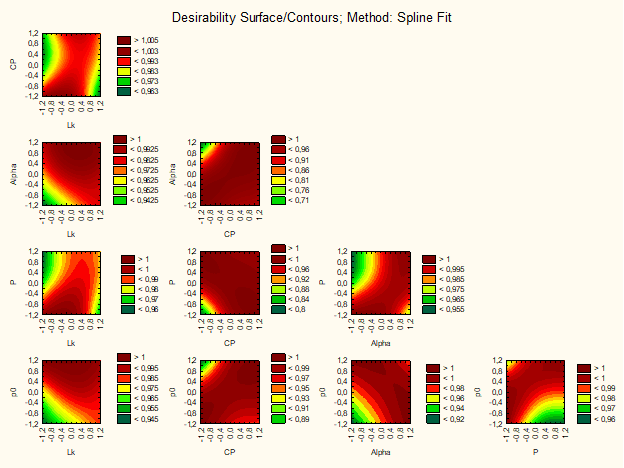
\includegraphics[width=1\textwidth]{P1M1_NGV_makespan_DSC}
\end{figure}

\begin{table}[]
\caption{Effect Estimates; Var.:Tempo; R-sqr=0,98992; Adj:0,98729; 5 3-level factors, 1 Blocks, 243 Runs; MS Residual=1,459374; DV: Tempo. Modelo 1, problema de \textit{makespan}}
\label{tab:P1M1_NGV_tempo}
\hspace*{-1.2cm} % shift left (tune the value)
\resizebox{1.2\textwidth}{!}{% scale relative to textwidth
\begin{tabular}{lllllllllll}
\rowcolor[HTML]{FFFFFF} 
{\color[HTML]{000000} Factors}        & {\color[HTML]{000000} Effect}   & {\color[HTML]{000000} Std.Err}  & {\color[HTML]{000000} t(192)}    & {\color[HTML]{000000} p}        & {\color[HTML]{000000} -95\% Cnf.Limt} & {\color[HTML]{000000} +95\% Cnf.Limt} & {\color[HTML]{000000} Coeff.}   & {\color[HTML]{000000} Std.Err.Coeff} & {\color[HTML]{000000} -95\% Cnf.Limt} & {\color[HTML]{000000} +95\% Cnf.Limt} \\
\rowcolor[HTML]{FFFFFF} 
{\color[HTML]{000000} Mean/Interc.}   & {\color[HTML]{FF0000} 12,13253} & {\color[HTML]{FF0000} 0,077496} & {\color[HTML]{FF0000} 156,5565} & {\color[HTML]{FF0000} 0,000000} & {\color[HTML]{FF0000} 11,97967}       & {\color[HTML]{FF0000} 12,28538}       & {\color[HTML]{FF0000} 12,13253} & {\color[HTML]{FF0000} 0,077496}      & {\color[HTML]{FF0000} 11,97967}       & {\color[HTML]{FF0000} 12,28538}       \\
\rowcolor[HTML]{FFFFFF} 
{\color[HTML]{000000} (1)Lk      (L)} & {\color[HTML]{FF0000} 13,62214} & {\color[HTML]{FF0000} 0,189826} & {\color[HTML]{FF0000} 71,7612}  & {\color[HTML]{FF0000} 0,000000} & {\color[HTML]{FF0000} 13,24772}       & {\color[HTML]{FF0000} 13,99655}       & {\color[HTML]{FF0000} 6,81107}  & {\color[HTML]{FF0000} 0,094913}      & {\color[HTML]{FF0000} 6,62386}        & {\color[HTML]{FF0000} 6,99827}        \\
\rowcolor[HTML]{FFFFFF} 
{\color[HTML]{000000} Lk      (Q)}    & {\color[HTML]{FF0000} 1,16790}  & {\color[HTML]{FF0000} 0,164394} & {\color[HTML]{FF0000} 7,1043}   & {\color[HTML]{FF0000} 0,000000} & {\color[HTML]{FF0000} 0,84365}        & {\color[HTML]{FF0000} 1,49215}        & {\color[HTML]{FF0000} 0,58395}  & {\color[HTML]{FF0000} 0,082197}      & {\color[HTML]{FF0000} 0,42182}        & {\color[HTML]{FF0000} 0,74607}        \\
\rowcolor[HTML]{FFFFFF} 
{\color[HTML]{000000} (2)CP      (L)} & {\color[HTML]{FF0000} 19,62236} & {\color[HTML]{FF0000} 0,189826} & {\color[HTML]{FF0000} 103,3702} & {\color[HTML]{FF0000} 0,000000} & {\color[HTML]{FF0000} 19,24795}       & {\color[HTML]{FF0000} 19,99678}       & {\color[HTML]{FF0000} 9,81118}  & {\color[HTML]{FF0000} 0,094913}      & {\color[HTML]{FF0000} 9,62398}        & {\color[HTML]{FF0000} 9,99839}        \\
\rowcolor[HTML]{FFFFFF} 
{\color[HTML]{000000} CP      (Q)}    & {\color[HTML]{FF0000} 1,66684}  & {\color[HTML]{FF0000} 0,164394} & {\color[HTML]{FF0000} 10,1393}  & {\color[HTML]{FF0000} 0,000000} & {\color[HTML]{FF0000} 1,34259}        & {\color[HTML]{FF0000} 1,99109}        & {\color[HTML]{FF0000} 0,83342}  & {\color[HTML]{FF0000} 0,082197}      & {\color[HTML]{FF0000} 0,67130}        & {\color[HTML]{FF0000} 0,99555}        \\
\rowcolor[HTML]{FFFFFF} 
{\color[HTML]{000000} (3)Alpha   (L)} & {\color[HTML]{FF0000} 0,68372}  & {\color[HTML]{FF0000} 0,189826} & {\color[HTML]{FF0000} 3,6018}   & {\color[HTML]{FF0000} 0,000402} & {\color[HTML]{FF0000} 0,30931}        & {\color[HTML]{FF0000} 1,05813}        & {\color[HTML]{FF0000} 0,34186}  & {\color[HTML]{FF0000} 0,094913}      & {\color[HTML]{FF0000} 0,15465}        & {\color[HTML]{FF0000} 0,52907}        \\
\rowcolor[HTML]{FFFFFF} 
{\color[HTML]{000000} Alpha   (Q)}    & {\color[HTML]{181A1B} -0,11882} & {\color[HTML]{181A1B} 0,164394} & {\color[HTML]{181A1B} -0,7228}  & {\color[HTML]{181A1B} 0,470684} & {\color[HTML]{181A1B} -0,44307}       & {\color[HTML]{181A1B} 0,20543}        & {\color[HTML]{181A1B} -0,05941} & {\color[HTML]{181A1B} 0,082197}      & {\color[HTML]{181A1B} -0,22154}       & {\color[HTML]{181A1B} 0,10271}        \\
\rowcolor[HTML]{FFFFFF} 
{\color[HTML]{000000} (4)P       (L)} & {\color[HTML]{FF0000} 3,48910}  & {\color[HTML]{FF0000} 0,189826} & {\color[HTML]{FF0000} 18,3805}  & {\color[HTML]{FF0000} 0,000000} & {\color[HTML]{FF0000} 3,11468}        & {\color[HTML]{FF0000} 3,86351}        & {\color[HTML]{FF0000} 1,74455}  & {\color[HTML]{FF0000} 0,094913}      & {\color[HTML]{FF0000} 1,55734}        & {\color[HTML]{FF0000} 1,93175}        \\
\rowcolor[HTML]{FFFFFF} 
{\color[HTML]{000000} P       (Q)}    & {\color[HTML]{FF0000} 1,27850}  & {\color[HTML]{FF0000} 0,164394} & {\color[HTML]{FF0000} 7,7771}   & {\color[HTML]{FF0000} 0,000000} & {\color[HTML]{FF0000} 0,95425}        & {\color[HTML]{FF0000} 1,60276}        & {\color[HTML]{FF0000} 0,63925}  & {\color[HTML]{FF0000} 0,082197}      & {\color[HTML]{FF0000} 0,47713}        & {\color[HTML]{FF0000} 0,80138}        \\
\rowcolor[HTML]{FFFFFF} 
{\color[HTML]{000000} (5)p0      (L)} & {\color[HTML]{181A1B} 0,23432}  & {\color[HTML]{181A1B} 0,189826} & {\color[HTML]{181A1B} 1,2344}   & {\color[HTML]{181A1B} 0,218574} & {\color[HTML]{181A1B} -0,14010}       & {\color[HTML]{181A1B} 0,60873}        & {\color[HTML]{181A1B} 0,11716}  & {\color[HTML]{181A1B} 0,094913}      & {\color[HTML]{181A1B} -0,07005}       & {\color[HTML]{181A1B} 0,30436}        \\
\rowcolor[HTML]{FFFFFF} 
{\color[HTML]{000000} p0      (Q)}    & {\color[HTML]{181A1B} 0,15427}  & {\color[HTML]{181A1B} 0,164394} & {\color[HTML]{181A1B} 0,9384}   & {\color[HTML]{181A1B} 0,349205} & {\color[HTML]{181A1B} -0,16998}       & {\color[HTML]{181A1B} 0,47852}        & {\color[HTML]{181A1B} 0,07714}  & {\color[HTML]{181A1B} 0,082197}      & {\color[HTML]{181A1B} -0,08499}       & {\color[HTML]{181A1B} 0,23926}        \\
\rowcolor[HTML]{FFFFFF} 
{\color[HTML]{000000} 1L by 2L}       & {\color[HTML]{FF0000} 10,28914} & {\color[HTML]{FF0000} 0,232488} & {\color[HTML]{FF0000} 44,2565}  & {\color[HTML]{FF0000} 0,000000} & {\color[HTML]{FF0000} 9,83058}        & {\color[HTML]{FF0000} 10,74770}       & {\color[HTML]{FF0000} 5,14457}  & {\color[HTML]{FF0000} 0,116244}      & {\color[HTML]{FF0000} 4,91529}        & {\color[HTML]{FF0000} 5,37385}        \\
\rowcolor[HTML]{FFFFFF} 
{\color[HTML]{000000} 1L by 2Q}       & {\color[HTML]{FF0000} 1,77548}  & {\color[HTML]{FF0000} 0,201341} & {\color[HTML]{FF0000} 8,8183}   & {\color[HTML]{FF0000} 0,000000} & {\color[HTML]{FF0000} 1,37836}        & {\color[HTML]{FF0000} 2,17261}        & {\color[HTML]{FF0000} 0,88774}  & {\color[HTML]{FF0000} 0,100670}      & {\color[HTML]{FF0000} 0,68918}        & {\color[HTML]{FF0000} 1,08630}        \\
\rowcolor[HTML]{FFFFFF} 
{\color[HTML]{000000} 1Q by 2L}       & {\color[HTML]{FF0000} 1,16728}  & {\color[HTML]{FF0000} 0,201341} & {\color[HTML]{FF0000} 5,7975}   & {\color[HTML]{FF0000} 0,000000} & {\color[HTML]{FF0000} 0,77016}        & {\color[HTML]{FF0000} 1,56440}        & {\color[HTML]{FF0000} 0,58364}  & {\color[HTML]{FF0000} 0,100670}      & {\color[HTML]{FF0000} 0,38508}        & {\color[HTML]{FF0000} 0,78220}        \\
\rowcolor[HTML]{FFFFFF} 
{\color[HTML]{000000} 1Q by 2Q}       & {\color[HTML]{181A1B} -0,23543} & {\color[HTML]{181A1B} 0,174366} & {\color[HTML]{181A1B} -1,3502}  & {\color[HTML]{181A1B} 0,178536} & {\color[HTML]{181A1B} -0,57935}       & {\color[HTML]{181A1B} 0,10849}        & {\color[HTML]{181A1B} -0,11772} & {\color[HTML]{181A1B} 0,087183}      & {\color[HTML]{181A1B} -0,28968}       & {\color[HTML]{181A1B} 0,05424}        \\
\rowcolor[HTML]{FFFFFF} 
{\color[HTML]{000000} 1L by 3L}       & {\color[HTML]{181A1B} 0,45376}  & {\color[HTML]{181A1B} 0,232488} & {\color[HTML]{181A1B} 1,9517}   & {\color[HTML]{181A1B} 0,052424} & {\color[HTML]{181A1B} -0,00480}       & {\color[HTML]{181A1B} 0,91232}        & {\color[HTML]{181A1B} 0,22688}  & {\color[HTML]{181A1B} 0,116244}      & {\color[HTML]{181A1B} -0,00240}       & {\color[HTML]{181A1B} 0,45616}        \\
\rowcolor[HTML]{FFFFFF} 
{\color[HTML]{000000} 1L by 3Q}       & {\color[HTML]{181A1B} -0,09508} & {\color[HTML]{181A1B} 0,201341} & {\color[HTML]{181A1B} -0,4722}  & {\color[HTML]{181A1B} 0,637297} & {\color[HTML]{181A1B} -0,49220}       & {\color[HTML]{181A1B} 0,30204}        & {\color[HTML]{181A1B} -0,04754} & {\color[HTML]{181A1B} 0,100670}      & {\color[HTML]{181A1B} -0,24610}       & {\color[HTML]{181A1B} 0,15102}        \\
\rowcolor[HTML]{FFFFFF} 
{\color[HTML]{000000} 1Q by 3L}       & {\color[HTML]{181A1B} -0,02559} & {\color[HTML]{181A1B} 0,201341} & {\color[HTML]{181A1B} -0,1271}  & {\color[HTML]{181A1B} 0,898978} & {\color[HTML]{181A1B} -0,42272}       & {\color[HTML]{181A1B} 0,37153}        & {\color[HTML]{181A1B} -0,01280} & {\color[HTML]{181A1B} 0,100670}      & {\color[HTML]{181A1B} -0,21136}       & {\color[HTML]{181A1B} 0,18576}        \\
\rowcolor[HTML]{FFFFFF} 
{\color[HTML]{000000} 1Q by 3Q}       & {\color[HTML]{181A1B} 0,17401}  & {\color[HTML]{181A1B} 0,174366} & {\color[HTML]{181A1B} 0,9980}   & {\color[HTML]{181A1B} 0,319545} & {\color[HTML]{181A1B} -0,16991}       & {\color[HTML]{181A1B} 0,51793}        & {\color[HTML]{181A1B} 0,08701}  & {\color[HTML]{181A1B} 0,087183}      & {\color[HTML]{181A1B} -0,08495}       & {\color[HTML]{181A1B} 0,25897}        \\
\rowcolor[HTML]{FFFFFF} 
{\color[HTML]{000000} 1L by 4L}       & {\color[HTML]{FF0000} 2,39385}  & {\color[HTML]{FF0000} 0,232488} & {\color[HTML]{FF0000} 10,2966}  & {\color[HTML]{FF0000} 0,000000} & {\color[HTML]{FF0000} 1,93529}        & {\color[HTML]{FF0000} 2,85241}        & {\color[HTML]{FF0000} 1,19692}  & {\color[HTML]{FF0000} 0,116244}      & {\color[HTML]{FF0000} 0,96764}        & {\color[HTML]{FF0000} 1,42620}        \\
\rowcolor[HTML]{FFFFFF} 
{\color[HTML]{000000} 1L by 4Q}       & {\color[HTML]{FF0000} 1,09805}  & {\color[HTML]{FF0000} 0,201341} & {\color[HTML]{FF0000} 5,4537}   & {\color[HTML]{FF0000} 0,000000} & {\color[HTML]{FF0000} 0,70092}        & {\color[HTML]{FF0000} 1,49517}        & {\color[HTML]{FF0000} 0,54902}  & {\color[HTML]{FF0000} 0,100670}      & {\color[HTML]{FF0000} 0,35046}        & {\color[HTML]{FF0000} 0,74759}        \\
\rowcolor[HTML]{FFFFFF} 
{\color[HTML]{000000} 1Q by 4L}       & {\color[HTML]{181A1B} 0,11748}  & {\color[HTML]{181A1B} 0,201341} & {\color[HTML]{181A1B} 0,5835}   & {\color[HTML]{181A1B} 0,560255} & {\color[HTML]{181A1B} -0,27965}       & {\color[HTML]{181A1B} 0,51460}        & {\color[HTML]{181A1B} 0,05874}  & {\color[HTML]{181A1B} 0,100670}      & {\color[HTML]{181A1B} -0,13982}       & {\color[HTML]{181A1B} 0,25730}        \\
\rowcolor[HTML]{FFFFFF} 
{\color[HTML]{000000} 1Q by 4Q}       & {\color[HTML]{181A1B} -0,11948} & {\color[HTML]{181A1B} 0,174366} & {\color[HTML]{181A1B} -0,6852}  & {\color[HTML]{181A1B} 0,494026} & {\color[HTML]{181A1B} -0,46340}       & {\color[HTML]{181A1B} 0,22444}        & {\color[HTML]{181A1B} -0,05974} & {\color[HTML]{181A1B} 0,087183}      & {\color[HTML]{181A1B} -0,23170}       & {\color[HTML]{181A1B} 0,11222}        \\
\rowcolor[HTML]{FFFFFF} 
{\color[HTML]{000000} 1L by 5L}       & {\color[HTML]{181A1B} 0,17933}  & {\color[HTML]{181A1B} 0,232488} & {\color[HTML]{181A1B} 0,7713}   & {\color[HTML]{181A1B} 0,441453} & {\color[HTML]{181A1B} -0,27923}       & {\color[HTML]{181A1B} 0,63789}        & {\color[HTML]{181A1B} 0,08966}  & {\color[HTML]{181A1B} 0,116244}      & {\color[HTML]{181A1B} -0,13962}       & {\color[HTML]{181A1B} 0,31894}        \\
\rowcolor[HTML]{FFFFFF} 
{\color[HTML]{000000} 1L by 5Q}       & {\color[HTML]{181A1B} 0,22357}  & {\color[HTML]{181A1B} 0,201341} & {\color[HTML]{181A1B} 1,1104}   & {\color[HTML]{181A1B} 0,268218} & {\color[HTML]{181A1B} -0,17356}       & {\color[HTML]{181A1B} 0,62069}        & {\color[HTML]{181A1B} 0,11178}  & {\color[HTML]{181A1B} 0,100670}      & {\color[HTML]{181A1B} -0,08678}       & {\color[HTML]{181A1B} 0,31035}        \\
\rowcolor[HTML]{FFFFFF} 
{\color[HTML]{000000} 1Q by 5L}       & {\color[HTML]{181A1B} -0,11632} & {\color[HTML]{181A1B} 0,201341} & {\color[HTML]{181A1B} -0,5777}  & {\color[HTML]{181A1B} 0,564118} & {\color[HTML]{181A1B} -0,51345}       & {\color[HTML]{181A1B} 0,28080}        & {\color[HTML]{181A1B} -0,05816} & {\color[HTML]{181A1B} 0,100670}      & {\color[HTML]{181A1B} -0,25672}       & {\color[HTML]{181A1B} 0,14040}        \\
\rowcolor[HTML]{FFFFFF} 
{\color[HTML]{000000} 1Q by 5Q}       & {\color[HTML]{181A1B} 0,02635}  & {\color[HTML]{181A1B} 0,174366} & {\color[HTML]{181A1B} 0,1511}   & {\color[HTML]{181A1B} 0,880036} & {\color[HTML]{181A1B} -0,31757}       & {\color[HTML]{181A1B} 0,37027}        & {\color[HTML]{181A1B} 0,01318}  & {\color[HTML]{181A1B} 0,087183}      & {\color[HTML]{181A1B} -0,15878}       & {\color[HTML]{181A1B} 0,18514}        \\
\rowcolor[HTML]{FFFFFF} 
{\color[HTML]{000000} 2L by 3L}       & {\color[HTML]{FF0000} 1,74960}  & {\color[HTML]{FF0000} 0,232488} & {\color[HTML]{FF0000} 7,5255}   & {\color[HTML]{FF0000} 0,000000} & {\color[HTML]{FF0000} 1,29104}        & {\color[HTML]{FF0000} 2,20816}        & {\color[HTML]{FF0000} 0,87480}  & {\color[HTML]{FF0000} 0,116244}      & {\color[HTML]{FF0000} 0,64552}        & {\color[HTML]{FF0000} 1,10408}        \\
\rowcolor[HTML]{FFFFFF} 
{\color[HTML]{000000} 2L by 3Q}       & {\color[HTML]{FF0000} -0,54684} & {\color[HTML]{FF0000} 0,201341} & {\color[HTML]{FF0000} -2,7160}  & {\color[HTML]{FF0000} 0,007211} & {\color[HTML]{FF0000} -0,94397}       & {\color[HTML]{FF0000} -0,14972}       & {\color[HTML]{FF0000} -0,27342} & {\color[HTML]{FF0000} 0,100670}      & {\color[HTML]{FF0000} -0,47198}       & {\color[HTML]{FF0000} -0,07486}       \\
\rowcolor[HTML]{FFFFFF} 
{\color[HTML]{000000} 2Q by 3L}       & {\color[HTML]{FF0000} 0,75124}  & {\color[HTML]{FF0000} 0,201341} & {\color[HTML]{FF0000} 3,7312}   & {\color[HTML]{FF0000} 0,000251} & {\color[HTML]{FF0000} 0,35411}        & {\color[HTML]{FF0000} 1,14836}        & {\color[HTML]{FF0000} 0,37562}  & {\color[HTML]{FF0000} 0,100670}      & {\color[HTML]{FF0000} 0,17706}        & {\color[HTML]{FF0000} 0,57418}        \\
\rowcolor[HTML]{FFFFFF} 
{\color[HTML]{000000} 2Q by 3Q}       & {\color[HTML]{181A1B} -0,33750} & {\color[HTML]{181A1B} 0,174366} & {\color[HTML]{181A1B} -1,9356}  & {\color[HTML]{181A1B} 0,054385} & {\color[HTML]{181A1B} -0,68142}       & {\color[HTML]{181A1B} 0,00642}        & {\color[HTML]{181A1B} -0,16875} & {\color[HTML]{181A1B} 0,087183}      & {\color[HTML]{181A1B} -0,34071}       & {\color[HTML]{181A1B} 0,00321}        \\
\rowcolor[HTML]{FFFFFF} 
{\color[HTML]{000000} 2L by 4L}       & {\color[HTML]{FF0000} 2,25720}  & {\color[HTML]{FF0000} 0,232488} & {\color[HTML]{FF0000} 9,7089}   & {\color[HTML]{FF0000} 0,000000} & {\color[HTML]{FF0000} 1,79864}        & {\color[HTML]{FF0000} 2,71576}        & {\color[HTML]{FF0000} 1,12860}  & {\color[HTML]{FF0000} 0,116244}      & {\color[HTML]{FF0000} 0,89932}        & {\color[HTML]{FF0000} 1,35788}        \\
\rowcolor[HTML]{FFFFFF} 
{\color[HTML]{000000} 2L by 4Q}       & {\color[HTML]{FF0000} 0,96528}  & {\color[HTML]{FF0000} 0,201341} & {\color[HTML]{FF0000} 4,7942}   & {\color[HTML]{FF0000} 0,000003} & {\color[HTML]{FF0000} 0,56815}        & {\color[HTML]{FF0000} 1,36240}        & {\color[HTML]{FF0000} 0,48264}  & {\color[HTML]{FF0000} 0,100670}      & {\color[HTML]{FF0000} 0,28408}        & {\color[HTML]{FF0000} 0,68120}        \\
\rowcolor[HTML]{FFFFFF} 
2Q by 4L                              & {\color[HTML]{FF0000} 0,53284}  & {\color[HTML]{FF0000} 0,201341} & {\color[HTML]{FF0000} 2,6465}   & {\color[HTML]{FF0000} 0,008809} & {\color[HTML]{FF0000} 0,13572}        & {\color[HTML]{FF0000} 0,92997}        & {\color[HTML]{FF0000} 0,26642}  & {\color[HTML]{FF0000} 0,100670}      & {\color[HTML]{FF0000} 0,06786}        & {\color[HTML]{FF0000} 0,46498}        \\
\rowcolor[HTML]{FFFFFF} 
2Q by 4Q                              & {\color[HTML]{181A1B} -0,01009} & {\color[HTML]{181A1B} 0,174366} & {\color[HTML]{181A1B} -0,0579}  & {\color[HTML]{181A1B} 0,953909} & {\color[HTML]{181A1B} -0,35401}       & {\color[HTML]{181A1B} 0,33383}        & {\color[HTML]{181A1B} -0,00505} & {\color[HTML]{181A1B} 0,087183}      & {\color[HTML]{181A1B} -0,17701}       & {\color[HTML]{181A1B} 0,16691}        \\
\rowcolor[HTML]{FFFFFF} 
2L by 5L                              & {\color[HTML]{181A1B} 0,40344}  & {\color[HTML]{181A1B} 0,232488} & {\color[HTML]{181A1B} 1,7353}   & {\color[HTML]{181A1B} 0,084290} & {\color[HTML]{181A1B} -0,05512}       & {\color[HTML]{181A1B} 0,86200}        & {\color[HTML]{181A1B} 0,20172}  & {\color[HTML]{181A1B} 0,116244}      & {\color[HTML]{181A1B} -0,02756}       & {\color[HTML]{181A1B} 0,43100}        \\
\rowcolor[HTML]{FFFFFF} 
2L by 5Q                              & {\color[HTML]{181A1B} 0,16409}  & {\color[HTML]{181A1B} 0,201341} & {\color[HTML]{181A1B} 0,8150}   & {\color[HTML]{181A1B} 0,416084} & {\color[HTML]{181A1B} -0,23303}       & {\color[HTML]{181A1B} 0,56122}        & {\color[HTML]{181A1B} 0,08205}  & {\color[HTML]{181A1B} 0,100670}      & {\color[HTML]{181A1B} -0,11652}       & {\color[HTML]{181A1B} 0,28061}        \\
\rowcolor[HTML]{FFFFFF} 
2Q by 5L                              & {\color[HTML]{181A1B} 0,07408}  & {\color[HTML]{181A1B} 0,201341} & {\color[HTML]{181A1B} 0,3680}   & {\color[HTML]{181A1B} 0,713316} & {\color[HTML]{181A1B} -0,32304}       & {\color[HTML]{181A1B} 0,47121}        & {\color[HTML]{181A1B} 0,03704}  & {\color[HTML]{181A1B} 0,100670}      & {\color[HTML]{181A1B} -0,16152}       & {\color[HTML]{181A1B} 0,23560}        \\
\rowcolor[HTML]{FFFFFF} 
2Q by 5Q                              & {\color[HTML]{181A1B} -0,25198} & {\color[HTML]{181A1B} 0,174366} & {\color[HTML]{181A1B} -1,4451}  & {\color[HTML]{181A1B} 0,150051} & {\color[HTML]{181A1B} -0,59590}       & {\color[HTML]{181A1B} 0,09194}        & {\color[HTML]{181A1B} -0,12599} & {\color[HTML]{181A1B} 0,087183}      & {\color[HTML]{181A1B} -0,29795}       & {\color[HTML]{181A1B} 0,04597}        \\
\rowcolor[HTML]{FFFFFF} 
3L by 4L                              & {\color[HTML]{181A1B} 0,33507}  & {\color[HTML]{181A1B} 0,232488} & {\color[HTML]{181A1B} 1,4412}   & {\color[HTML]{181A1B} 0,151145} & {\color[HTML]{181A1B} -0,12349}       & {\color[HTML]{181A1B} 0,79363}        & {\color[HTML]{181A1B} 0,16754}  & {\color[HTML]{181A1B} 0,116244}      & {\color[HTML]{181A1B} -0,06174}       & {\color[HTML]{181A1B} 0,39682}        \\
\rowcolor[HTML]{FFFFFF} 
3L by 4Q                              & {\color[HTML]{181A1B} 0,23495}  & {\color[HTML]{181A1B} 0,201341} & {\color[HTML]{181A1B} 1,1669}   & {\color[HTML]{181A1B} 0,244687} & {\color[HTML]{181A1B} -0,16217}       & {\color[HTML]{181A1B} 0,63207}        & {\color[HTML]{181A1B} 0,11748}  & {\color[HTML]{181A1B} 0,100670}      & {\color[HTML]{181A1B} -0,08109}       & {\color[HTML]{181A1B} 0,31604}        \\
\rowcolor[HTML]{FFFFFF} 
3Q by 4L                              & {\color[HTML]{181A1B} -0,21669} & {\color[HTML]{181A1B} 0,201341} & {\color[HTML]{181A1B} -1,0763}  & {\color[HTML]{181A1B} 0,283162} & {\color[HTML]{181A1B} -0,61382}       & {\color[HTML]{181A1B} 0,18043}        & {\color[HTML]{181A1B} -0,10835} & {\color[HTML]{181A1B} 0,100670}      & {\color[HTML]{181A1B} -0,30691}       & {\color[HTML]{181A1B} 0,09021}        \\
\rowcolor[HTML]{FFFFFF} 
3Q by 4Q                              & {\color[HTML]{181A1B} 0,07438}  & {\color[HTML]{181A1B} 0,174366} & {\color[HTML]{181A1B} 0,4266}   & {\color[HTML]{181A1B} 0,670168} & {\color[HTML]{181A1B} -0,26954}       & {\color[HTML]{181A1B} 0,41830}        & {\color[HTML]{181A1B} 0,03719}  & {\color[HTML]{181A1B} 0,087183}      & {\color[HTML]{181A1B} -0,13477}       & {\color[HTML]{181A1B} 0,20915}        \\
\rowcolor[HTML]{FFFFFF} 
3L by 5L                              & {\color[HTML]{FF0000} 0,50616}  & {\color[HTML]{FF0000} 0,232488} & {\color[HTML]{FF0000} 2,1771}   & {\color[HTML]{FF0000} 0,030691} & {\color[HTML]{FF0000} 0,04760}        & {\color[HTML]{FF0000} 0,96472}        & {\color[HTML]{FF0000} 0,25308}  & {\color[HTML]{FF0000} 0,116244}      & {\color[HTML]{FF0000} 0,02380}        & {\color[HTML]{FF0000} 0,48236}        \\
\rowcolor[HTML]{FFFFFF} 
3L by 5Q                              & {\color[HTML]{181A1B} -0,29040} & {\color[HTML]{181A1B} 0,201341} & {\color[HTML]{181A1B} -1,4423}  & {\color[HTML]{181A1B} 0,150845} & {\color[HTML]{181A1B} -0,68752}       & {\color[HTML]{181A1B} 0,10673}        & {\color[HTML]{181A1B} -0,14520} & {\color[HTML]{181A1B} 0,100670}      & {\color[HTML]{181A1B} -0,34376}       & {\color[HTML]{181A1B} 0,05336}        \\
\rowcolor[HTML]{FFFFFF} 
3Q by 5L                              & {\color[HTML]{181A1B} -0,34815} & {\color[HTML]{181A1B} 0,201341} & {\color[HTML]{181A1B} -1,7292}  & {\color[HTML]{181A1B} 0,085384} & {\color[HTML]{181A1B} -0,74528}       & {\color[HTML]{181A1B} 0,04897}        & {\color[HTML]{181A1B} -0,17408} & {\color[HTML]{181A1B} 0,100670}      & {\color[HTML]{181A1B} -0,37264}       & {\color[HTML]{181A1B} 0,02448}        \\
\rowcolor[HTML]{FFFFFF} 
3Q by 5Q                              & {\color[HTML]{181A1B} -0,19125} & {\color[HTML]{181A1B} 0,174366} & {\color[HTML]{181A1B} -1,0968}  & {\color[HTML]{181A1B} 0,274093} & {\color[HTML]{181A1B} -0,53517}       & {\color[HTML]{181A1B} 0,15267}        & {\color[HTML]{181A1B} -0,09562} & {\color[HTML]{181A1B} 0,087183}      & {\color[HTML]{181A1B} -0,26758}       & {\color[HTML]{181A1B} 0,07634}        \\
\rowcolor[HTML]{FFFFFF} 
4L by 5L                              & {\color[HTML]{181A1B} 0,19665}  & {\color[HTML]{181A1B} 0,232488} & {\color[HTML]{181A1B} 0,8458}   & {\color[HTML]{181A1B} 0,398697} & {\color[HTML]{181A1B} -0,26191}       & {\color[HTML]{181A1B} 0,65521}        & {\color[HTML]{181A1B} 0,09832}  & {\color[HTML]{181A1B} 0,116244}      & {\color[HTML]{181A1B} -0,13096}       & {\color[HTML]{181A1B} 0,32760}        \\
\rowcolor[HTML]{FFFFFF} 
4L by 5Q                              & {\color[HTML]{181A1B} -0,28064} & {\color[HTML]{181A1B} 0,201341} & {\color[HTML]{181A1B} -1,3938}  & {\color[HTML]{181A1B} 0,164975} & {\color[HTML]{181A1B} -0,67776}       & {\color[HTML]{181A1B} 0,11649}        & {\color[HTML]{181A1B} -0,14032} & {\color[HTML]{181A1B} 0,100670}      & {\color[HTML]{181A1B} -0,33888}       & {\color[HTML]{181A1B} 0,05824}        \\
\rowcolor[HTML]{FFFFFF} 
4Q by 5L                              & {\color[HTML]{181A1B} 0,16679}  & {\color[HTML]{181A1B} 0,201341} & {\color[HTML]{181A1B} 0,8284}   & {\color[HTML]{181A1B} 0,408467} & {\color[HTML]{181A1B} -0,23033}       & {\color[HTML]{181A1B} 0,56392}        & {\color[HTML]{181A1B} 0,08340}  & {\color[HTML]{181A1B} 0,100670}      & {\color[HTML]{181A1B} -0,11517}       & {\color[HTML]{181A1B} 0,28196}        \\
\rowcolor[HTML]{FFFFFF} 
4Q by 5Q                              & {\color[HTML]{181A1B} -0,02010} & {\color[HTML]{181A1B} 0,174366} & {\color[HTML]{181A1B} -0,1153}  & {\color[HTML]{181A1B} 0,908333} & {\color[HTML]{181A1B} -0,36402}       & {\color[HTML]{181A1B} 0,32382}        & {\color[HTML]{181A1B} -0,01005} & {\color[HTML]{181A1B} 0,087183}      & {\color[HTML]{181A1B} -0,18201}       & {\color[HTML]{181A1B} 0,16191}       
\end{tabular}
}
\end{table}

\begin{figure}[H]
\caption{Gráfico de contorno das cinco variáveis ($L_{k}$, $CP$, $\alpha$, $P$, $p_{0}$), relativamente ao tempo, do Modelo 1 do problema de \textit{makespan}}
\centering
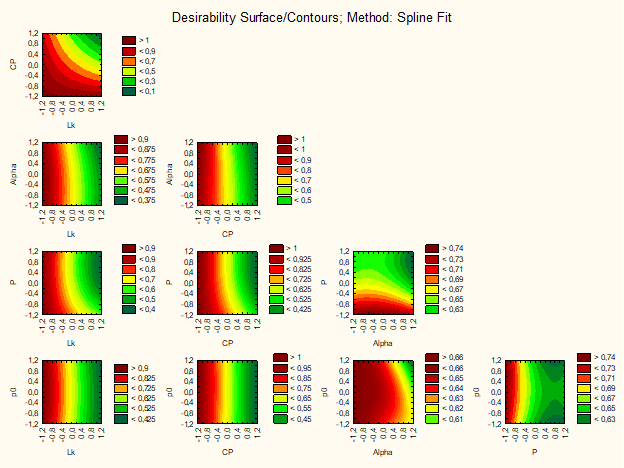
\includegraphics[width=1\textwidth]{P1M1_NGV_tempo_DSC}
\end{figure}



\begin{table}[H]
\caption{Effect Estimates; Var.:Makespan; R-sqr=0,79905; Adj:0,66508 ; 4 3-level factors, 1 Blocks, 81 Runs; MS Residual=29,81784; DV: Makespan. Modelo 2, problema de \textit{makespan}}
\label{tab:P1M1_GV_makespan}
\hspace*{-1.2cm} % shift left (tune the value)
\resizebox{1.2\textwidth}{!}{% scale relative to textwidth
\begin{tabular}{lllllllllll}
\rowcolor[HTML]{FFFFFF} 
{\color[HTML]{000000} Factors}        & {\color[HTML]{000000} Effect}   & {\color[HTML]{000000} Std.Err}  & {\color[HTML]{000000} t(48)}    & {\color[HTML]{000000} p}        & {\color[HTML]{000000} -95\% Cnf.Limt} & {\color[HTML]{000000} +95\% Cnf.Limt} & {\color[HTML]{000000} Coeff.}   & {\color[HTML]{000000} Std.Err.Coeff} & {\color[HTML]{000000} -95\% Cnf.Limt} & {\color[HTML]{000000} +95\% Cnf.Limt} \\
\rowcolor[HTML]{FFFFFF} 
{\color[HTML]{000000} Mean/Interc.}   & {\color[HTML]{FF0000} 512,7222} & {\color[HTML]{FF0000} 0,606730} & {\color[HTML]{FF0000} 845,0581} & {\color[HTML]{FF0000} 0,000000} & {\color[HTML]{FF0000} 511,5023}       & {\color[HTML]{FF0000} 513,9421}       & {\color[HTML]{FF0000} 512,7222} & {\color[HTML]{FF0000} 0,606730}      & {\color[HTML]{FF0000} 511,5023}       & {\color[HTML]{FF0000} 513,9421}       \\
\rowcolor[HTML]{FFFFFF} 
{\color[HTML]{000000} (1)Lk      (L)} & {\color[HTML]{FF0000} -9,3259}  & {\color[HTML]{FF0000} 1,486179} & {\color[HTML]{FF0000} -6,2751}  & {\color[HTML]{FF0000} 0,000000} & {\color[HTML]{FF0000} -12,3141}       & {\color[HTML]{FF0000} -6,3378}        & {\color[HTML]{FF0000} -4,6630}  & {\color[HTML]{FF0000} 0,743090}      & {\color[HTML]{FF0000} -6,1570}        & {\color[HTML]{FF0000} -3,1689}        \\
\rowcolor[HTML]{FFFFFF} 
{\color[HTML]{000000} Lk      (Q)}    & {\color[HTML]{000000} -2,1111}  & {\color[HTML]{000000} 1,287069} & {\color[HTML]{000000} -1,6402}  & {\color[HTML]{000000} 0,107492} & {\color[HTML]{000000} -4,6989}        & {\color[HTML]{000000} 0,4767}         & {\color[HTML]{000000} -1,0556}  & {\color[HTML]{000000} 0,643535}      & {\color[HTML]{000000} -2,3495}        & {\color[HTML]{000000} 0,2384}         \\
\rowcolor[HTML]{FFFFFF} 
{\color[HTML]{000000} (2)CP      (L)} & {\color[HTML]{FF0000} -10,9111} & {\color[HTML]{FF0000} 1,486179} & {\color[HTML]{FF0000} -7,3417}  & {\color[HTML]{FF0000} 0,000000} & {\color[HTML]{FF0000} -13,8993}       & {\color[HTML]{FF0000} -7,9229}        & {\color[HTML]{FF0000} -5,4556}  & {\color[HTML]{FF0000} 0,743090}      & {\color[HTML]{FF0000} -6,9496}        & {\color[HTML]{FF0000} -3,9615}        \\
\rowcolor[HTML]{FFFFFF} 
{\color[HTML]{000000} CP      (Q)}    & {\color[HTML]{FF0000} -4,9667}  & {\color[HTML]{FF0000} 1,287069} & {\color[HTML]{FF0000} -3,8589}  & {\color[HTML]{FF0000} 0,000340} & {\color[HTML]{FF0000} -7,5545}        & {\color[HTML]{FF0000} -2,3788}        & {\color[HTML]{FF0000} -2,4833}  & {\color[HTML]{FF0000} 0,643535}      & {\color[HTML]{FF0000} -3,7772}        & {\color[HTML]{FF0000} -1,1894}        \\
\rowcolor[HTML]{FFFFFF} 
{\color[HTML]{000000} (3)Alpha   (L)} & {\color[HTML]{000000} 0,5667}   & {\color[HTML]{000000} 1,486179} & {\color[HTML]{000000} 0,3813}   & {\color[HTML]{000000} 0,704670} & {\color[HTML]{000000} -2,4215}        & {\color[HTML]{000000} 3,5548}         & {\color[HTML]{000000} 0,2833}   & {\color[HTML]{000000} 0,743090}      & {\color[HTML]{000000} -1,2107}        & {\color[HTML]{000000} 1,7774}         \\
\rowcolor[HTML]{FFFFFF} 
{\color[HTML]{000000} Alpha   (Q)}    & {\color[HTML]{000000} -1,2167}  & {\color[HTML]{000000} 1,287069} & {\color[HTML]{000000} -0,9453}  & {\color[HTML]{000000} 0,349240} & {\color[HTML]{000000} -3,8045}        & {\color[HTML]{000000} 1,3712}         & {\color[HTML]{000000} -0,6083}  & {\color[HTML]{000000} 0,643535}      & {\color[HTML]{000000} -1,9022}        & {\color[HTML]{000000} 0,6856}         \\
\rowcolor[HTML]{FFFFFF} 
{\color[HTML]{000000} (4)p0      (L)} & {\color[HTML]{000000} 0,6815}   & {\color[HTML]{000000} 1,486179} & {\color[HTML]{000000} 0,4585}   & {\color[HTML]{000000} 0,648630} & {\color[HTML]{000000} -2,3067}        & {\color[HTML]{000000} 3,6696}         & {\color[HTML]{000000} 0,3407}   & {\color[HTML]{000000} 0,743090}      & {\color[HTML]{000000} -1,1533}        & {\color[HTML]{000000} 1,8348}         \\
\rowcolor[HTML]{FFFFFF} 
{\color[HTML]{000000} p0      (Q)}    & {\color[HTML]{000000} -2,0889}  & {\color[HTML]{000000} 1,287069} & {\color[HTML]{000000} -1,6230}  & {\color[HTML]{000000} 0,111144} & {\color[HTML]{000000} -4,6767}        & {\color[HTML]{000000} 0,4989}         & {\color[HTML]{000000} -1,0444}  & {\color[HTML]{000000} 0,643535}      & {\color[HTML]{000000} -2,3384}        & {\color[HTML]{000000} 0,2495}         \\
\rowcolor[HTML]{FFFFFF} 
{\color[HTML]{000000} 1L by 2L}       & {\color[HTML]{FF0000} 7,4889}   & {\color[HTML]{FF0000} 1,820190} & {\color[HTML]{FF0000} 4,1143}   & {\color[HTML]{FF0000} 0,000152} & {\color[HTML]{FF0000} 3,8292}         & {\color[HTML]{FF0000} 11,1486}        & {\color[HTML]{FF0000} 3,7444}   & {\color[HTML]{FF0000} 0,910095}      & {\color[HTML]{FF0000} 1,9146}         & {\color[HTML]{FF0000} 5,5743}         \\
\rowcolor[HTML]{FFFFFF} 
{\color[HTML]{000000} 1L by 2Q}       & {\color[HTML]{FF0000} 3,2444}   & {\color[HTML]{FF0000} 1,576331} & {\color[HTML]{FF0000} 2,0582}   & {\color[HTML]{FF0000} 0,045020} & {\color[HTML]{FF0000} 0,0750}         & {\color[HTML]{FF0000} 6,4139}         & {\color[HTML]{FF0000} 1,6222}   & {\color[HTML]{FF0000} 0,788166}      & {\color[HTML]{FF0000} 0,0375}         & {\color[HTML]{FF0000} 3,2069}         \\
\rowcolor[HTML]{FFFFFF} 
{\color[HTML]{000000} 1Q by 2L}       & {\color[HTML]{000000} 2,3500}   & {\color[HTML]{000000} 1,576331} & {\color[HTML]{000000} 1,4908}   & {\color[HTML]{000000} 0,142556} & {\color[HTML]{000000} -0,8194}        & {\color[HTML]{000000} 5,5194}         & {\color[HTML]{000000} 1,1750}   & {\color[HTML]{000000} 0,788166}      & {\color[HTML]{000000} -0,4097}        & {\color[HTML]{000000} 2,7597}         \\
\rowcolor[HTML]{FFFFFF} 
{\color[HTML]{000000} 1Q by 2Q}       & {\color[HTML]{000000} 0,9083}   & {\color[HTML]{000000} 1,365143} & {\color[HTML]{000000} 0,6654}   & {\color[HTML]{000000} 0,508995} & {\color[HTML]{000000} -1,8365}        & {\color[HTML]{000000} 3,6531}         & {\color[HTML]{000000} 0,4542}   & {\color[HTML]{000000} 0,682571}      & {\color[HTML]{000000} -0,9182}        & {\color[HTML]{000000} 1,8266}         \\
\rowcolor[HTML]{FFFFFF} 
{\color[HTML]{000000} 1L by 3L}       & {\color[HTML]{000000} -2,2556}  & {\color[HTML]{000000} 1,820190} & {\color[HTML]{000000} -1,2392}  & {\color[HTML]{000000} 0,221302} & {\color[HTML]{000000} -5,9153}        & {\color[HTML]{000000} 1,4042}         & {\color[HTML]{000000} -1,1278}  & {\color[HTML]{000000} 0,910095}      & {\color[HTML]{000000} -2,9576}        & {\color[HTML]{000000} 0,7021}         \\
\rowcolor[HTML]{FFFFFF} 
{\color[HTML]{000000} 1L by 3Q}       & {\color[HTML]{000000} 0,5111}   & {\color[HTML]{000000} 1,576331} & {\color[HTML]{000000} 0,3242}   & {\color[HTML]{000000} 0,747164} & {\color[HTML]{000000} -2,6583}        & {\color[HTML]{000000} 3,6805}         & {\color[HTML]{000000} 0,2556}   & {\color[HTML]{000000} 0,788166}      & {\color[HTML]{000000} -1,3292}        & {\color[HTML]{000000} 1,8403}         \\
\rowcolor[HTML]{FFFFFF} 
{\color[HTML]{000000} 1Q by 3L}       & {\color[HTML]{000000} -0,6667}  & {\color[HTML]{000000} 1,576331} & {\color[HTML]{000000} -0,4229}  & {\color[HTML]{000000} 0,674240} & {\color[HTML]{000000} -3,8361}        & {\color[HTML]{000000} 2,5028}         & {\color[HTML]{000000} -0,3333}  & {\color[HTML]{000000} 0,788166}      & {\color[HTML]{000000} -1,9180}        & {\color[HTML]{000000} 1,2514}         \\
\rowcolor[HTML]{FFFFFF} 
{\color[HTML]{000000} 1Q by 3Q}       & {\color[HTML]{000000} -0,0417}  & {\color[HTML]{000000} 1,365143} & {\color[HTML]{000000} -0,0305}  & {\color[HTML]{000000} 0,975777} & {\color[HTML]{000000} -2,7865}        & {\color[HTML]{000000} 2,7031}         & {\color[HTML]{000000} -0,0208}  & {\color[HTML]{000000} 0,682571}      & {\color[HTML]{000000} -1,3932}        & {\color[HTML]{000000} 1,3516}         \\
\rowcolor[HTML]{FFFFFF} 
{\color[HTML]{000000} 1L by 4L}       & {\color[HTML]{000000} -2,9222}  & {\color[HTML]{000000} 1,820190} & {\color[HTML]{000000} -1,6054}  & {\color[HTML]{000000} 0,114955} & {\color[HTML]{000000} -6,5820}        & {\color[HTML]{000000} 0,7375}         & {\color[HTML]{000000} -1,4611}  & {\color[HTML]{000000} 0,910095}      & {\color[HTML]{000000} -3,2910}        & {\color[HTML]{000000} 0,3688}         \\
\rowcolor[HTML]{FFFFFF} 
{\color[HTML]{000000} 1L by 4Q}       & {\color[HTML]{000000} 0,2444}   & {\color[HTML]{000000} 1,576331} & {\color[HTML]{000000} 0,1551}   & {\color[HTML]{000000} 0,877415} & {\color[HTML]{000000} -2,9250}        & {\color[HTML]{000000} 3,4139}         & {\color[HTML]{000000} 0,1222}   & {\color[HTML]{000000} 0,788166}      & {\color[HTML]{000000} -1,4625}        & {\color[HTML]{000000} 1,7069}         \\
\rowcolor[HTML]{FFFFFF} 
{\color[HTML]{000000} 1Q by 4L}       & {\color[HTML]{000000} 0,3889}   & {\color[HTML]{000000} 1,576331} & {\color[HTML]{000000} 0,2467}   & {\color[HTML]{000000} 0,806189} & {\color[HTML]{000000} -2,7805}        & {\color[HTML]{000000} 3,5583}         & {\color[HTML]{000000} 0,1944}   & {\color[HTML]{000000} 0,788166}      & {\color[HTML]{000000} -1,3903}        & {\color[HTML]{000000} 1,7792}         \\
\rowcolor[HTML]{FFFFFF} 
{\color[HTML]{000000} 1Q by 4Q}       & {\color[HTML]{000000} 0,2250}   & {\color[HTML]{000000} 1,365143} & {\color[HTML]{000000} 0,1648}   & {\color[HTML]{000000} 0,869779} & {\color[HTML]{000000} -2,5198}        & {\color[HTML]{000000} 2,9698}         & {\color[HTML]{000000} 0,1125}   & {\color[HTML]{000000} 0,682571}      & {\color[HTML]{000000} -1,2599}        & {\color[HTML]{000000} 1,4849}         \\
\rowcolor[HTML]{FFFFFF} 
{\color[HTML]{000000} 2L by 3L}       & {\color[HTML]{FF0000} -5,8333}  & {\color[HTML]{FF0000} 1,820190} & {\color[HTML]{FF0000} -3,2048}  & {\color[HTML]{FF0000} 0,002404} & {\color[HTML]{FF0000} -9,4931}        & {\color[HTML]{FF0000} -2,1736}        & {\color[HTML]{FF0000} -2,9167}  & {\color[HTML]{FF0000} 0,910095}      & {\color[HTML]{FF0000} -4,7465}        & {\color[HTML]{FF0000} -1,0868}        \\
\rowcolor[HTML]{FFFFFF} 
{\color[HTML]{000000} 2L by 3Q}       & {\color[HTML]{FF0000} 3,3500}   & {\color[HTML]{FF0000} 1,576331} & {\color[HTML]{FF0000} 2,1252}   & {\color[HTML]{FF0000} 0,038745} & {\color[HTML]{FF0000} 0,1806}         & {\color[HTML]{FF0000} 6,5194}         & {\color[HTML]{FF0000} 1,6750}   & {\color[HTML]{FF0000} 0,788166}      & {\color[HTML]{FF0000} 0,0903}         & {\color[HTML]{FF0000} 3,2597}         \\
\rowcolor[HTML]{FFFFFF} 
{\color[HTML]{000000} 2Q by 3L}       & {\color[HTML]{000000} -2,9667}  & {\color[HTML]{000000} 1,576331} & {\color[HTML]{000000} -1,8820}  & {\color[HTML]{000000} 0,065905} & {\color[HTML]{000000} -6,1361}        & {\color[HTML]{000000} 0,2028}         & {\color[HTML]{000000} -1,4833}  & {\color[HTML]{000000} 0,788166}      & {\color[HTML]{000000} -3,0680}        & {\color[HTML]{000000} 0,1014}         \\
\rowcolor[HTML]{FFFFFF} 
{\color[HTML]{000000} 2Q by 3Q}       & {\color[HTML]{000000} 1,6500}   & {\color[HTML]{000000} 1,365143} & {\color[HTML]{000000} 1,2087}   & {\color[HTML]{000000} 0,232712} & {\color[HTML]{000000} -1,0948}        & {\color[HTML]{000000} 4,3948}         & {\color[HTML]{000000} 0,8250}   & {\color[HTML]{000000} 0,682571}      & {\color[HTML]{000000} -0,5474}        & {\color[HTML]{000000} 2,1974}         \\
\rowcolor[HTML]{FFFFFF} 
{\color[HTML]{000000} 2L by 4L}       & {\color[HTML]{FF0000} -5,1444}  & {\color[HTML]{FF0000} 1,820190} & {\color[HTML]{FF0000} -2,8263}  & {\color[HTML]{FF0000} 0,006844} & {\color[HTML]{FF0000} -8,8042}        & {\color[HTML]{FF0000} -1,4847}        & {\color[HTML]{FF0000} -2,5722}  & {\color[HTML]{FF0000} 0,910095}      & {\color[HTML]{FF0000} -4,4021}        & {\color[HTML]{FF0000} -0,7424}        \\
\rowcolor[HTML]{FFFFFF} 
{\color[HTML]{000000} 2L by 4Q}       & {\color[HTML]{000000} 2,9167}   & {\color[HTML]{000000} 1,576331} & {\color[HTML]{000000} 1,8503}   & {\color[HTML]{000000} 0,070432} & {\color[HTML]{000000} -0,2528}        & {\color[HTML]{000000} 6,0861}         & {\color[HTML]{000000} 1,4583}   & {\color[HTML]{000000} 0,788166}      & {\color[HTML]{000000} -0,1264}        & {\color[HTML]{000000} 3,0430}         \\
\rowcolor[HTML]{FFFFFF} 
{\color[HTML]{000000} 2Q by 4L}       & {\color[HTML]{000000} -2,5111}  & {\color[HTML]{000000} 1,576331} & {\color[HTML]{000000} -1,5930}  & {\color[HTML]{000000} 0,117723} & {\color[HTML]{000000} -5,6805}        & {\color[HTML]{000000} 0,6583}         & {\color[HTML]{000000} -1,2556}  & {\color[HTML]{000000} 0,788166}      & {\color[HTML]{000000} -2,8403}        & {\color[HTML]{000000} 0,3292}         \\
\rowcolor[HTML]{FFFFFF} 
{\color[HTML]{000000} 2Q by 4Q}       & {\color[HTML]{000000} 1,4667}   & {\color[HTML]{000000} 1,365143} & {\color[HTML]{000000} 1,0744}   & {\color[HTML]{000000} 0,288029} & {\color[HTML]{000000} -1,2781}        & {\color[HTML]{000000} 4,2115}         & {\color[HTML]{000000} 0,7333}   & {\color[HTML]{000000} 0,682571}      & {\color[HTML]{000000} -0,6391}        & {\color[HTML]{000000} 2,1057}         \\
\rowcolor[HTML]{FFFFFF} 
{\color[HTML]{000000} 3L by 4L}       & {\color[HTML]{FF0000} 3,7111}   & {\color[HTML]{FF0000} 1,820190} & {\color[HTML]{FF0000} 2,0389}   & {\color[HTML]{FF0000} 0,046992} & {\color[HTML]{FF0000} 0,0514}         & {\color[HTML]{FF0000} 7,3708}         & {\color[HTML]{FF0000} 1,8556}   & {\color[HTML]{FF0000} 0,910095}      & {\color[HTML]{FF0000} 0,0257}         & {\color[HTML]{FF0000} 3,6854}         \\
\rowcolor[HTML]{FFFFFF} 
{\color[HTML]{000000} 3L by 4Q}       & {\color[HTML]{FF0000} -4,2167}  & {\color[HTML]{FF0000} 1,576331} & {\color[HTML]{FF0000} -2,6750}  & {\color[HTML]{FF0000} 0,010189} & {\color[HTML]{FF0000} -7,3861}        & {\color[HTML]{FF0000} -1,0472}        & {\color[HTML]{FF0000} -2,1083}  & {\color[HTML]{FF0000} 0,788166}      & {\color[HTML]{FF0000} -3,6930}        & {\color[HTML]{FF0000} -0,5236}        \\
\rowcolor[HTML]{FFFFFF} 
{\color[HTML]{000000} 3Q by 4L}       & {\color[HTML]{000000} -1,5944}  & {\color[HTML]{000000} 1,576331} & {\color[HTML]{000000} -1,0115}  & {\color[HTML]{000000} 0,316853} & {\color[HTML]{000000} -4,7639}        & {\color[HTML]{000000} 1,5750}         & {\color[HTML]{000000} -0,7972}  & {\color[HTML]{000000} 0,788166}      & {\color[HTML]{000000} -2,3819}        & {\color[HTML]{000000} 0,7875}         \\
\rowcolor[HTML]{FFFFFF} 
{\color[HTML]{000000} 3Q by 4Q}       & {\color[HTML]{000000} 1,0167}   & {\color[HTML]{000000} 1,365143} & {\color[HTML]{000000} 0,7447}   & {\color[HTML]{000000} 0,460064} & {\color[HTML]{000000} -1,7281}        & {\color[HTML]{000000} 3,7615}         & {\color[HTML]{000000} 0,5083}   & {\color[HTML]{000000} 0,682571}      & {\color[HTML]{000000} -0,8641}        & {\color[HTML]{000000} 1,8807}        
\end{tabular}
}
\end{table}

\begin{figure}[H]
\caption{Gráfico de contorno das quatro variáveis relevantes ($L_{k}$, $CP$, $\alpha$, $p_{0}$), relativamente ao \textit{makespan}, do Modelo 2 do problema de \textit{makespan}}
\centering
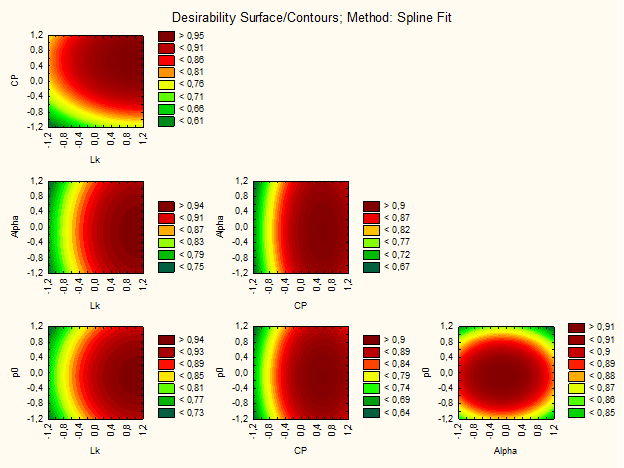
\includegraphics[width=1\textwidth]{P1M1_GV_makespan_DSC}
\end{figure}


\begin{table}[H]
\caption{Effect Estimates; Var.:Tempo; R-sqr=0,97985; Adj:0,96642; 4 3-level factors, 1 Blocks, 81 Runs; MS Residual=5,912985; DV: Tempo. Modelo 2, problema de \textit{makespan}}
\label{tab:P1M1_GV_tempo}
\hspace*{-1.2cm} % shift left (tune the value)
\resizebox{1.2\textwidth}{!}{% scale relative to textwidth
\begin{tabular}{lllllllllll}
\rowcolor[HTML]{FFFFFF} 
{\color[HTML]{000000} Factors}        & {\color[HTML]{000000} Effect}   & {\color[HTML]{000000} Std.Err}  & {\color[HTML]{000000} t(48)}    & {\color[HTML]{000000} p}        & {\color[HTML]{000000} -95\% Cnf.Limt} & {\color[HTML]{000000} +95\% Cnf.Limt} & {\color[HTML]{000000} Coeff.}   & {\color[HTML]{000000} Std.Err.Coeff} & {\color[HTML]{000000} -95\% Cnf.Limt} & {\color[HTML]{000000} +95\% Cnf.Limt} \\
\rowcolor[HTML]{FFFFFF} 
{\color[HTML]{000000} Mean/Interc.}   & {\color[HTML]{FF0000} 19,94905} & {\color[HTML]{FF0000} 0,270185} & {\color[HTML]{FF0000} 73,83485} & {\color[HTML]{FF0000} 0,000000} & {\color[HTML]{FF0000} 19,40581}       & {\color[HTML]{FF0000} 20,49229}       & {\color[HTML]{FF0000} 19,94905} & {\color[HTML]{FF0000} 0,270185}      & {\color[HTML]{FF0000} 19,40581}       & {\color[HTML]{FF0000} 20,49229}       \\
\rowcolor[HTML]{FFFFFF} 
{\color[HTML]{000000} (1)Lk      (L)} & {\color[HTML]{FF0000} 21,72384} & {\color[HTML]{FF0000} 0,661815} & {\color[HTML]{FF0000} 32,82465} & {\color[HTML]{FF0000} 0,000000} & {\color[HTML]{FF0000} 20,39317}       & {\color[HTML]{FF0000} 23,05451}       & {\color[HTML]{FF0000} 10,86192} & {\color[HTML]{FF0000} 0,330907}      & {\color[HTML]{FF0000} 10,19659}       & {\color[HTML]{FF0000} 11,52725}       \\
\rowcolor[HTML]{FFFFFF} 
{\color[HTML]{000000} Lk      (Q)}    & {\color[HTML]{000000} 0,72651}  & {\color[HTML]{000000} 0,573148} & {\color[HTML]{000000} 1,26758}  & {\color[HTML]{000000} 0,211063} & {\color[HTML]{000000} -0,42588}       & {\color[HTML]{000000} 1,87890}        & {\color[HTML]{000000} 0,36326}  & {\color[HTML]{000000} 0,286574}      & {\color[HTML]{000000} -0,21294}       & {\color[HTML]{000000} 0,93945}        \\
\rowcolor[HTML]{FFFFFF} 
{\color[HTML]{000000} (2)CP      (L)} & {\color[HTML]{FF0000} 19,97500} & {\color[HTML]{FF0000} 0,661815} & {\color[HTML]{FF0000} 30,18215} & {\color[HTML]{FF0000} 0,000000} & {\color[HTML]{FF0000} 18,64433}       & {\color[HTML]{FF0000} 21,30566}       & {\color[HTML]{FF0000} 9,98750}  & {\color[HTML]{FF0000} 0,330907}      & {\color[HTML]{FF0000} 9,32216}        & {\color[HTML]{FF0000} 10,65283}       \\
\rowcolor[HTML]{FFFFFF} 
{\color[HTML]{000000} CP      (Q)}    & {\color[HTML]{FF0000} 2,84850}  & {\color[HTML]{FF0000} 0,573148} & {\color[HTML]{FF0000} 4,96991}  & {\color[HTML]{FF0000} 0,000009} & {\color[HTML]{FF0000} 1,69611}        & {\color[HTML]{FF0000} 4,00089}        & {\color[HTML]{FF0000} 1,42425}  & {\color[HTML]{FF0000} 0,286574}      & {\color[HTML]{FF0000} 0,84805}        & {\color[HTML]{FF0000} 2,00045}        \\
\rowcolor[HTML]{FFFFFF} 
{\color[HTML]{000000} (3)Alpha   (L)} & {\color[HTML]{FF0000} 3,31104}  & {\color[HTML]{FF0000} 0,661815} & {\color[HTML]{FF0000} 5,00297}  & {\color[HTML]{FF0000} 0,000008} & {\color[HTML]{FF0000} 1,98037}        & {\color[HTML]{FF0000} 4,64170}        & {\color[HTML]{FF0000} 1,65552}  & {\color[HTML]{FF0000} 0,330907}      & {\color[HTML]{FF0000} 0,99018}        & {\color[HTML]{FF0000} 2,32085}        \\
\rowcolor[HTML]{FFFFFF} 
{\color[HTML]{000000} Alpha   (Q)}    & {\color[HTML]{000000} -1,14631} & {\color[HTML]{000000} 0,573148} & {\color[HTML]{000000} -2,00001} & {\color[HTML]{000000} 0,051174} & {\color[HTML]{000000} -2,29870}       & {\color[HTML]{000000} 0,00609}        & {\color[HTML]{000000} -0,57315} & {\color[HTML]{000000} 0,286574}      & {\color[HTML]{000000} -1,14935}       & {\color[HTML]{000000} 0,00304}        \\
\rowcolor[HTML]{FFFFFF} 
{\color[HTML]{000000} (4)p0      (L)} & {\color[HTML]{FF0000} 2,11030}  & {\color[HTML]{FF0000} 0,661815} & {\color[HTML]{FF0000} 3,18866}  & {\color[HTML]{FF0000} 0,002517} & {\color[HTML]{FF0000} 0,77964}        & {\color[HTML]{FF0000} 3,44097}        & {\color[HTML]{FF0000} 1,05515}  & {\color[HTML]{FF0000} 0,330907}      & {\color[HTML]{FF0000} 0,38982}        & {\color[HTML]{FF0000} 1,72049}        \\
\rowcolor[HTML]{FFFFFF} 
{\color[HTML]{000000} p0      (Q)}    & {\color[HTML]{000000} -1,01754} & {\color[HTML]{000000} 0,573148} & {\color[HTML]{000000} -1,77534} & {\color[HTML]{000000} 0,082182} & {\color[HTML]{000000} -2,16993}       & {\color[HTML]{000000} 0,13486}        & {\color[HTML]{000000} -0,50877} & {\color[HTML]{000000} 0,286574}      & {\color[HTML]{000000} -1,08496}       & {\color[HTML]{000000} 0,06743}        \\
\rowcolor[HTML]{FFFFFF} 
{\color[HTML]{000000} 1L by 2L}       & {\color[HTML]{FF0000} 11,26922} & {\color[HTML]{FF0000} 0,810554} & {\color[HTML]{FF0000} 13,90310} & {\color[HTML]{FF0000} 0,000000} & {\color[HTML]{FF0000} 9,63949}        & {\color[HTML]{FF0000} 12,89895}       & {\color[HTML]{FF0000} 5,63461}  & {\color[HTML]{FF0000} 0,405277}      & {\color[HTML]{FF0000} 4,81975}        & {\color[HTML]{FF0000} 6,44947}        \\
\rowcolor[HTML]{FFFFFF} 
{\color[HTML]{000000} 1L by 2Q}       & {\color[HTML]{000000} 1,29787}  & {\color[HTML]{000000} 0,701961} & {\color[HTML]{000000} 1,84892}  & {\color[HTML]{000000} 0,070633} & {\color[HTML]{000000} -0,11352}       & {\color[HTML]{000000} 2,70926}        & {\color[HTML]{000000} 0,64894}  & {\color[HTML]{000000} 0,350980}      & {\color[HTML]{000000} -0,05676}       & {\color[HTML]{000000} 1,35463}        \\
\rowcolor[HTML]{FFFFFF} 
{\color[HTML]{000000} 1Q by 2L}       & {\color[HTML]{000000} 0,03951}  & {\color[HTML]{000000} 0,701961} & {\color[HTML]{000000} 0,05629}  & {\color[HTML]{000000} 0,955346} & {\color[HTML]{000000} -1,37187}       & {\color[HTML]{000000} 1,45090}        & {\color[HTML]{000000} 0,01976}  & {\color[HTML]{000000} 0,350980}      & {\color[HTML]{000000} -0,68594}       & {\color[HTML]{000000} 0,72545}        \\
\rowcolor[HTML]{FFFFFF} 
{\color[HTML]{000000} 1Q by 2Q}       & {\color[HTML]{000000} -0,11595} & {\color[HTML]{000000} 0,607916} & {\color[HTML]{000000} -0,19073} & {\color[HTML]{000000} 0,849543} & {\color[HTML]{000000} -1,33824}       & {\color[HTML]{000000} 1,10635}        & {\color[HTML]{000000} -0,05797} & {\color[HTML]{000000} 0,303958}      & {\color[HTML]{000000} -0,66912}       & {\color[HTML]{000000} 0,55318}        \\
\rowcolor[HTML]{FFFFFF} 
{\color[HTML]{000000} 1L by 3L}       & {\color[HTML]{FF0000} 4,36745}  & {\color[HTML]{FF0000} 0,810554} & {\color[HTML]{FF0000} 5,38822}  & {\color[HTML]{FF0000} 0,000002} & {\color[HTML]{FF0000} 2,73772}        & {\color[HTML]{FF0000} 5,99718}        & {\color[HTML]{FF0000} 2,18372}  & {\color[HTML]{FF0000} 0,405277}      & {\color[HTML]{FF0000} 1,36886}        & {\color[HTML]{FF0000} 2,99859}        \\
\rowcolor[HTML]{FFFFFF} 
{\color[HTML]{000000} 1L by 3Q}       & {\color[HTML]{FF0000} -1,49005} & {\color[HTML]{FF0000} 0,701961} & {\color[HTML]{FF0000} -2,12270} & {\color[HTML]{FF0000} 0,038963} & {\color[HTML]{FF0000} -2,90144}       & {\color[HTML]{FF0000} -0,07867}       & {\color[HTML]{FF0000} -0,74503} & {\color[HTML]{FF0000} 0,350980}      & {\color[HTML]{FF0000} -1,45072}       & {\color[HTML]{FF0000} -0,03933}       \\
\rowcolor[HTML]{FFFFFF} 
{\color[HTML]{000000} 1Q by 3L}       & {\color[HTML]{000000} -0,62145} & {\color[HTML]{000000} 0,701961} & {\color[HTML]{000000} -0,88530} & {\color[HTML]{000000} 0,380406} & {\color[HTML]{000000} -2,03284}       & {\color[HTML]{000000} 0,78994}        & {\color[HTML]{000000} -0,31072} & {\color[HTML]{000000} 0,350980}      & {\color[HTML]{000000} -1,01642}       & {\color[HTML]{000000} 0,39497}        \\
\rowcolor[HTML]{FFFFFF} 
{\color[HTML]{000000} 1Q by 3Q}       & {\color[HTML]{000000} -0,04126} & {\color[HTML]{000000} 0,607916} & {\color[HTML]{000000} -0,06787} & {\color[HTML]{000000} 0,946169} & {\color[HTML]{000000} -1,26356}       & {\color[HTML]{000000} 1,18104}        & {\color[HTML]{000000} -0,02063} & {\color[HTML]{000000} 0,303958}      & {\color[HTML]{000000} -0,63178}       & {\color[HTML]{000000} 0,59052}        \\
\rowcolor[HTML]{FFFFFF} 
{\color[HTML]{000000} 1L by 4L}       & {\color[HTML]{FF0000} 2,06900}  & {\color[HTML]{FF0000} 0,810554} & {\color[HTML]{FF0000} 2,55257}  & {\color[HTML]{FF0000} 0,013929} & {\color[HTML]{FF0000} 0,43927}        & {\color[HTML]{FF0000} 3,69873}        & {\color[HTML]{FF0000} 1,03450}  & {\color[HTML]{FF0000} 0,405277}      & {\color[HTML]{FF0000} 0,21963}        & {\color[HTML]{FF0000} 1,84936}        \\
\rowcolor[HTML]{FFFFFF} 
{\color[HTML]{000000} 1L by 4Q}       & {\color[HTML]{000000} -0,88475} & {\color[HTML]{000000} 0,701961} & {\color[HTML]{000000} -1,26039} & {\color[HTML]{000000} 0,213621} & {\color[HTML]{000000} -2,29613}       & {\color[HTML]{000000} 0,52664}        & {\color[HTML]{000000} -0,44237} & {\color[HTML]{000000} 0,350980}      & {\color[HTML]{000000} -1,14807}       & {\color[HTML]{000000} 0,26332}        \\
\rowcolor[HTML]{FFFFFF} 
{\color[HTML]{000000} 1Q by 4L}       & {\color[HTML]{000000} -0,12064} & {\color[HTML]{000000} 0,701961} & {\color[HTML]{000000} -0,17186} & {\color[HTML]{000000} 0,864271} & {\color[HTML]{000000} -1,53202}       & {\color[HTML]{000000} 1,29075}        & {\color[HTML]{000000} -0,06032} & {\color[HTML]{000000} 0,350980}      & {\color[HTML]{000000} -0,76601}       & {\color[HTML]{000000} 0,64537}        \\
\rowcolor[HTML]{FFFFFF} 
{\color[HTML]{000000} 1Q by 4Q}       & {\color[HTML]{000000} -0,25861} & {\color[HTML]{000000} 0,607916} & {\color[HTML]{000000} -0,42540} & {\color[HTML]{000000} 0,672449} & {\color[HTML]{000000} -1,48090}       & {\color[HTML]{000000} 0,96369}        & {\color[HTML]{000000} -0,12930} & {\color[HTML]{000000} 0,303958}      & {\color[HTML]{000000} -0,74045}       & {\color[HTML]{000000} 0,48185}        \\
\rowcolor[HTML]{FFFFFF} 
{\color[HTML]{000000} 2L by 3L}       & {\color[HTML]{FF0000} 2,11549}  & {\color[HTML]{FF0000} 0,810554} & {\color[HTML]{FF0000} 2,60993}  & {\color[HTML]{FF0000} 0,012043} & {\color[HTML]{FF0000} 0,48576}        & {\color[HTML]{FF0000} 3,74522}        & {\color[HTML]{FF0000} 1,05774}  & {\color[HTML]{FF0000} 0,405277}      & {\color[HTML]{FF0000} 0,24288}        & {\color[HTML]{FF0000} 1,87261}        \\
\rowcolor[HTML]{FFFFFF} 
{\color[HTML]{000000} 2L by 3Q}       & {\color[HTML]{000000} -0,84142} & {\color[HTML]{000000} 0,701961} & {\color[HTML]{000000} -1,19868} & {\color[HTML]{000000} 0,236538} & {\color[HTML]{000000} -2,25281}       & {\color[HTML]{000000} 0,56996}        & {\color[HTML]{000000} -0,42071} & {\color[HTML]{000000} 0,350980}      & {\color[HTML]{000000} -1,12641}       & {\color[HTML]{000000} 0,28498}        \\
\rowcolor[HTML]{FFFFFF} 
{\color[HTML]{000000} 2Q by 3L}       & {\color[HTML]{000000} 0,88890}  & {\color[HTML]{000000} 0,701961} & {\color[HTML]{000000} 1,26630}  & {\color[HTML]{000000} 0,211515} & {\color[HTML]{000000} -0,52249}       & {\color[HTML]{000000} 2,30028}        & {\color[HTML]{000000} 0,44445}  & {\color[HTML]{000000} 0,350980}      & {\color[HTML]{000000} -0,26125}       & {\color[HTML]{000000} 1,15014}        \\
\rowcolor[HTML]{FFFFFF} 
{\color[HTML]{000000} 2Q by 3Q}       & {\color[HTML]{000000} -0,55794} & {\color[HTML]{000000} 0,607916} & {\color[HTML]{000000} -0,91779} & {\color[HTML]{000000} 0,363316} & {\color[HTML]{000000} -1,78024}       & {\color[HTML]{000000} 0,66436}        & {\color[HTML]{000000} -0,27897} & {\color[HTML]{000000} 0,303958}      & {\color[HTML]{000000} -0,89012}       & {\color[HTML]{000000} 0,33218}        \\
\rowcolor[HTML]{FFFFFF} 
{\color[HTML]{000000} 2L by 4L}       & {\color[HTML]{000000} 0,63012}  & {\color[HTML]{000000} 0,810554} & {\color[HTML]{000000} 0,77740}  & {\color[HTML]{000000} 0,440738} & {\color[HTML]{000000} -0,99960}       & {\color[HTML]{000000} 2,25985}        & {\color[HTML]{000000} 0,31506}  & {\color[HTML]{000000} 0,405277}      & {\color[HTML]{000000} -0,49980}       & {\color[HTML]{000000} 1,12993}        \\
\rowcolor[HTML]{FFFFFF} 
{\color[HTML]{000000} 2L by 4Q}       & {\color[HTML]{000000} -0,42321} & {\color[HTML]{000000} 0,701961} & {\color[HTML]{000000} -0,60290} & {\color[HTML]{000000} 0,549415} & {\color[HTML]{000000} -1,83460}       & {\color[HTML]{000000} 0,98818}        & {\color[HTML]{000000} -0,21161} & {\color[HTML]{000000} 0,350980}      & {\color[HTML]{000000} -0,91730}       & {\color[HTML]{000000} 0,49409}        \\
\rowcolor[HTML]{FFFFFF} 
{\color[HTML]{000000} 2Q by 4L}       & {\color[HTML]{000000} 0,48816}  & {\color[HTML]{000000} 0,701961} & {\color[HTML]{000000} 0,69542}  & {\color[HTML]{000000} 0,490147} & {\color[HTML]{000000} -0,92323}       & {\color[HTML]{000000} 1,89954}        & {\color[HTML]{000000} 0,24408}  & {\color[HTML]{000000} 0,350980}      & {\color[HTML]{000000} -0,46162}       & {\color[HTML]{000000} 0,94977}        \\
\rowcolor[HTML]{FFFFFF} 
{\color[HTML]{000000} 2Q by 4Q}       & {\color[HTML]{000000} -0,17075} & {\color[HTML]{000000} 0,607916} & {\color[HTML]{000000} -0,28088} & {\color[HTML]{000000} 0,780006} & {\color[HTML]{000000} -1,39305}       & {\color[HTML]{000000} 1,05154}        & {\color[HTML]{000000} -0,08538} & {\color[HTML]{000000} 0,303958}      & {\color[HTML]{000000} -0,69653}       & {\color[HTML]{000000} 0,52577}        \\
\rowcolor[HTML]{FFFFFF} 
{\color[HTML]{000000} 3L by 4L}       & {\color[HTML]{FF0000} 3,86791}  & {\color[HTML]{FF0000} 0,810554} & {\color[HTML]{FF0000} 4,77193}  & {\color[HTML]{FF0000} 0,000017} & {\color[HTML]{FF0000} 2,23818}        & {\color[HTML]{FF0000} 5,49763}        & {\color[HTML]{FF0000} 1,93395}  & {\color[HTML]{FF0000} 0,405277}      & {\color[HTML]{FF0000} 1,11909}        & {\color[HTML]{FF0000} 2,74882}        \\
\rowcolor[HTML]{FFFFFF} 
{\color[HTML]{000000} 3L by 4Q}       & {\color[HTML]{000000} -0,61189} & {\color[HTML]{000000} 0,701961} & {\color[HTML]{000000} -0,87169} & {\color[HTML]{000000} 0,387719} & {\color[HTML]{000000} -2,02328}       & {\color[HTML]{000000} 0,79950}        & {\color[HTML]{000000} -0,30594} & {\color[HTML]{000000} 0,350980}      & {\color[HTML]{000000} -1,01164}       & {\color[HTML]{000000} 0,39975}        \\
\rowcolor[HTML]{FFFFFF} 
{\color[HTML]{000000} 3Q by 4L}       & {\color[HTML]{000000} -0,88585} & {\color[HTML]{000000} 0,701961} & {\color[HTML]{000000} -1,26197} & {\color[HTML]{000000} 0,213058} & {\color[HTML]{000000} -2,29724}       & {\color[HTML]{000000} 0,52553}        & {\color[HTML]{000000} -0,44293} & {\color[HTML]{000000} 0,350980}      & {\color[HTML]{000000} -1,14862}       & {\color[HTML]{000000} 0,26277}        \\
\rowcolor[HTML]{FFFFFF} 
{\color[HTML]{000000} 3Q by 4Q}       & {\color[HTML]{000000} 0,41730}  & {\color[HTML]{000000} 0,607916} & {\color[HTML]{000000} 0,68645}  & {\color[HTML]{000000} 0,495734} & {\color[HTML]{000000} -0,80499}       & {\color[HTML]{000000} 1,63960}        & {\color[HTML]{000000} 0,20865}  & {\color[HTML]{000000} 0,303958}      & {\color[HTML]{000000} -0,40250}       & {\color[HTML]{000000} 0,81980}       
\end{tabular}
}
\end{table}

\begin{figure}[H]
\caption{Gráfico de contorno das quatro variáveis relevantes ($L_{k}$, $CP$, $\alpha$, $p_{0}$), relativamente ao tempo, do Modelo 2 do problema de \textit{makespan}}
\centering
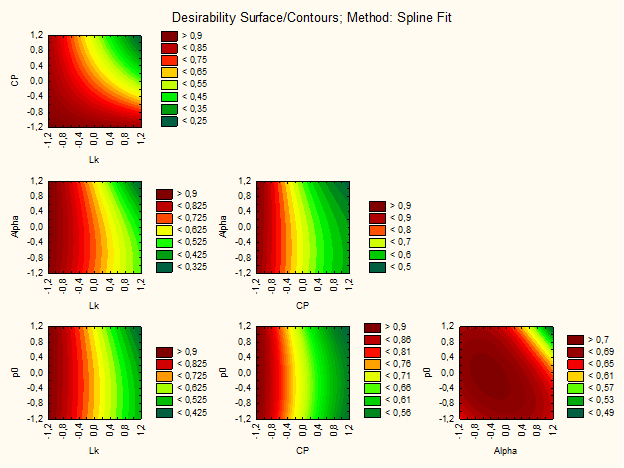
\includegraphics[width=1\textwidth]{P1M1_GV_tempo_DSC}
\end{figure}



\begin{table}[H]
\caption{Effect Estimates; Var.:Makespan; R-sqr=0,97227; Adj:0,95378; 4 3-level factors, 1 Blocks, 81 Runs; MS Residual=1,415756; DV: Makespan. Modelo 3, problema de \textit{makespan}}
\label{tab:P1M2_GV_makespan}
\hspace*{-1.2cm} % shift left (tune the value)
\resizebox{1.2\textwidth}{!}{% scale relative to textwidth
\begin{tabular}{
>{\columncolor[HTML]{FFFFFF}}l 
>{\columncolor[HTML]{FFFFFF}}l 
>{\columncolor[HTML]{FFFFFF}}l 
>{\columncolor[HTML]{FFFFFF}}l 
>{\columncolor[HTML]{FFFFFF}}l 
>{\columncolor[HTML]{FFFFFF}}l 
>{\columncolor[HTML]{FFFFFF}}l 
>{\columncolor[HTML]{FFFFFF}}l 
>{\columncolor[HTML]{FFFFFF}}l 
>{\columncolor[HTML]{FFFFFF}}l 
>{\columncolor[HTML]{FFFFFF}}l }
{\color[HTML]{000000} Factors}        & {\color[HTML]{000000} Effect}   & {\color[HTML]{000000} Std.Err}  & {\color[HTML]{000000} t(48)}    & {\color[HTML]{000000} p}        & {\color[HTML]{000000} -95\% Cnf.Limt} & {\color[HTML]{000000} +95\% Cnf.Limt} & {\color[HTML]{000000} Coeff.}   & {\color[HTML]{000000} Std.Err.Coeff} & {\color[HTML]{000000} -95\% Cnf.Limt} & {\color[HTML]{000000} +95\% Cnf.Limt} \\
{\color[HTML]{000000} Mean/Interc.}   & {\color[HTML]{FE0000} 501,4914} & {\color[HTML]{FE0000} 0,132206} & {\color[HTML]{FE0000} 3793,252} & {\color[HTML]{FE0000} 0,000000} & {\color[HTML]{FE0000} 501,2255}       & {\color[HTML]{FE0000} 501,7572}       & {\color[HTML]{FE0000} 501,4914} & {\color[HTML]{FE0000} 0,132206}      & {\color[HTML]{FE0000} 501,2255}       & {\color[HTML]{FE0000} 501,7572}       \\
{\color[HTML]{000000} (1)Lk      (L)} & {\color[HTML]{FE0000} -2,0185}  & {\color[HTML]{FE0000} 0,323838} & {\color[HTML]{FE0000} -6,233}   & {\color[HTML]{FE0000} 0,000000} & {\color[HTML]{FE0000} -2,6696}        & {\color[HTML]{FE0000} -1,3674}        & {\color[HTML]{FE0000} -1,0093}  & {\color[HTML]{FE0000} 0,161919}      & {\color[HTML]{FE0000} -1,3348}        & {\color[HTML]{FE0000} -0,6837}        \\
{\color[HTML]{000000} Lk      (Q)}    & {\color[HTML]{000000} -0,3537}  & {\color[HTML]{000000} 0,280452} & {\color[HTML]{000000} -1,261}   & {\color[HTML]{000000} 0,213335} & {\color[HTML]{000000} -0,9176}        & {\color[HTML]{000000} 0,2102}         & {\color[HTML]{000000} -0,1769}  & {\color[HTML]{000000} 0,140226}      & {\color[HTML]{000000} -0,4588}        & {\color[HTML]{000000} 0,1051}         \\
{\color[HTML]{000000} (2)CP      (L)} & {\color[HTML]{FE0000} -9,6630}  & {\color[HTML]{FE0000} 0,323838} & {\color[HTML]{FE0000} -29,839}  & {\color[HTML]{FE0000} 0,000000} & {\color[HTML]{FE0000} -10,3141}       & {\color[HTML]{FE0000} -9,0118}        & {\color[HTML]{FE0000} -4,8315}  & {\color[HTML]{FE0000} 0,161919}      & {\color[HTML]{FE0000} -5,1570}        & {\color[HTML]{FE0000} -4,5059}        \\
{\color[HTML]{000000} CP      (Q)}    & {\color[HTML]{FE0000} -3,7093}  & {\color[HTML]{FE0000} 0,280452} & {\color[HTML]{FE0000} -13,226}  & {\color[HTML]{FE0000} 0,000000} & {\color[HTML]{FE0000} -4,2731}        & {\color[HTML]{FE0000} -3,1454}        & {\color[HTML]{FE0000} -1,8546}  & {\color[HTML]{FE0000} 0,140226}      & {\color[HTML]{FE0000} -2,1366}        & {\color[HTML]{FE0000} -1,5727}        \\
{\color[HTML]{000000} (3)Alpha   (L)} & {\color[HTML]{FE0000} 4,6111}   & {\color[HTML]{FE0000} 0,323838} & {\color[HTML]{FE0000} 14,239}   & {\color[HTML]{FE0000} 0,000000} & {\color[HTML]{FE0000} 3,9600}         & {\color[HTML]{FE0000} 5,2622}         & {\color[HTML]{FE0000} 2,3056}   & {\color[HTML]{FE0000} 0,161919}      & {\color[HTML]{FE0000} 1,9800}         & {\color[HTML]{FE0000} 2,6311}         \\
{\color[HTML]{000000} Alpha   (Q)}    & {\color[HTML]{000000} -0,0759}  & {\color[HTML]{000000} 0,280452} & {\color[HTML]{000000} -0,271}   & {\color[HTML]{000000} 0,787762} & {\color[HTML]{000000} -0,6398}        & {\color[HTML]{000000} 0,4880}         & {\color[HTML]{000000} -0,0380}  & {\color[HTML]{000000} 0,140226}      & {\color[HTML]{000000} -0,3199}        & {\color[HTML]{000000} 0,2440}         \\
{\color[HTML]{000000} (4)p0      (L)} & {\color[HTML]{FE0000} 2,8481}   & {\color[HTML]{FE0000} 0,323838} & {\color[HTML]{FE0000} 8,795}    & {\color[HTML]{FE0000} 0,000000} & {\color[HTML]{FE0000} 2,1970}         & {\color[HTML]{FE0000} 3,4993}         & {\color[HTML]{FE0000} 1,4241}   & {\color[HTML]{FE0000} 0,161919}      & {\color[HTML]{FE0000} 1,0985}         & {\color[HTML]{FE0000} 1,7496}         \\
{\color[HTML]{000000} p0      (Q)}    & {\color[HTML]{000000} -0,0870}  & {\color[HTML]{000000} 0,280452} & {\color[HTML]{000000} -0,310}   & {\color[HTML]{000000} 0,757641} & {\color[HTML]{000000} -0,6509}        & {\color[HTML]{000000} 0,4768}         & {\color[HTML]{000000} -0,0435}  & {\color[HTML]{000000} 0,140226}      & {\color[HTML]{000000} -0,3255}        & {\color[HTML]{000000} 0,2384}         \\
{\color[HTML]{000000} 1L by 2L}       & {\color[HTML]{FE0000} 1,6611}   & {\color[HTML]{FE0000} 0,396619} & {\color[HTML]{FE0000} 4,188}    & {\color[HTML]{FE0000} 0,000120} & {\color[HTML]{FE0000} 0,8637}         & {\color[HTML]{FE0000} 2,4586}         & {\color[HTML]{FE0000} 0,8306}   & {\color[HTML]{FE0000} 0,198309}      & {\color[HTML]{FE0000} 0,4318}         & {\color[HTML]{FE0000} 1,2293}         \\
{\color[HTML]{000000} 1L by 2Q}       & {\color[HTML]{000000} 0,5306}   & {\color[HTML]{000000} 0,343482} & {\color[HTML]{000000} 1,545}    & {\color[HTML]{000000} 0,129001} & {\color[HTML]{000000} -0,1601}        & {\color[HTML]{000000} 1,2212}         & {\color[HTML]{000000} 0,2653}   & {\color[HTML]{000000} 0,171741}      & {\color[HTML]{000000} -0,0800}        & {\color[HTML]{000000} 0,6106}         \\
{\color[HTML]{000000} 1Q by 2L}       & {\color[HTML]{000000} -0,0861}  & {\color[HTML]{000000} 0,343482} & {\color[HTML]{000000} -0,251}   & {\color[HTML]{000000} 0,803116} & {\color[HTML]{000000} -0,7767}        & {\color[HTML]{000000} 0,6045}         & {\color[HTML]{000000} -0,0431}  & {\color[HTML]{000000} 0,171741}      & {\color[HTML]{000000} -0,3884}        & {\color[HTML]{000000} 0,3023}         \\
{\color[HTML]{000000} 1Q by 2Q}       & {\color[HTML]{000000} -0,1431}  & {\color[HTML]{000000} 0,297464} & {\color[HTML]{000000} -0,481}   & {\color[HTML]{000000} 0,632760} & {\color[HTML]{000000} -0,7411}        & {\color[HTML]{000000} 0,4550}         & {\color[HTML]{000000} -0,0715}  & {\color[HTML]{000000} 0,148732}      & {\color[HTML]{000000} -0,3706}        & {\color[HTML]{000000} 0,2275}         \\
{\color[HTML]{000000} 1L by 3L}       & {\color[HTML]{000000} -0,3889}  & {\color[HTML]{000000} 0,396619} & {\color[HTML]{000000} -0,981}   & {\color[HTML]{000000} 0,331750} & {\color[HTML]{000000} -1,1863}        & {\color[HTML]{000000} 0,4086}         & {\color[HTML]{000000} -0,1944}  & {\color[HTML]{000000} 0,198309}      & {\color[HTML]{000000} -0,5932}        & {\color[HTML]{000000} 0,2043}         \\
{\color[HTML]{000000} 1L by 3Q}       & {\color[HTML]{000000} 0,0556}   & {\color[HTML]{000000} 0,343482} & {\color[HTML]{000000} 0,162}    & {\color[HTML]{000000} 0,872188} & {\color[HTML]{000000} -0,6351}        & {\color[HTML]{000000} 0,7462}         & {\color[HTML]{000000} 0,0278}   & {\color[HTML]{000000} 0,171741}      & {\color[HTML]{000000} -0,3175}        & {\color[HTML]{000000} 0,3731}         \\
{\color[HTML]{000000} 1Q by 3L}       & {\color[HTML]{000000} -0,1167}  & {\color[HTML]{000000} 0,343482} & {\color[HTML]{000000} -0,340}   & {\color[HTML]{000000} 0,735595} & {\color[HTML]{000000} -0,8073}        & {\color[HTML]{000000} 0,5739}         & {\color[HTML]{000000} -0,0583}  & {\color[HTML]{000000} 0,171741}      & {\color[HTML]{000000} -0,4036}        & {\color[HTML]{000000} 0,2870}         \\
{\color[HTML]{000000} 1Q by 3Q}       & {\color[HTML]{000000} 0,1944}   & {\color[HTML]{000000} 0,297464} & {\color[HTML]{000000} 0,654}    & {\color[HTML]{000000} 0,516441} & {\color[HTML]{000000} -0,4036}        & {\color[HTML]{000000} 0,7925}         & {\color[HTML]{000000} 0,0972}   & {\color[HTML]{000000} 0,148732}      & {\color[HTML]{000000} -0,2018}        & {\color[HTML]{000000} 0,3963}         \\
{\color[HTML]{000000} 1L by 4L}       & {\color[HTML]{000000} 0,0833}   & {\color[HTML]{000000} 0,396619} & {\color[HTML]{000000} 0,210}    & {\color[HTML]{000000} 0,834472} & {\color[HTML]{000000} -0,7141}        & {\color[HTML]{000000} 0,8808}         & {\color[HTML]{000000} 0,0417}   & {\color[HTML]{000000} 0,198309}      & {\color[HTML]{000000} -0,3571}        & {\color[HTML]{000000} 0,4404}         \\
{\color[HTML]{000000} 1L by 4Q}       & {\color[HTML]{000000} -0,3528}  & {\color[HTML]{000000} 0,343482} & {\color[HTML]{000000} -1,027}   & {\color[HTML]{000000} 0,309538} & {\color[HTML]{000000} -1,0434}        & {\color[HTML]{000000} 0,3378}         & {\color[HTML]{000000} -0,1764}  & {\color[HTML]{000000} 0,171741}      & {\color[HTML]{000000} -0,5217}        & {\color[HTML]{000000} 0,1689}         \\
{\color[HTML]{000000} 1Q by 4L}       & {\color[HTML]{000000} 0,3639}   & {\color[HTML]{000000} 0,343482} & {\color[HTML]{000000} 1,059}    & {\color[HTML]{000000} 0,294714} & {\color[HTML]{000000} -0,3267}        & {\color[HTML]{000000} 1,0545}         & {\color[HTML]{000000} 0,1819}   & {\color[HTML]{000000} 0,171741}      & {\color[HTML]{000000} -0,1634}        & {\color[HTML]{000000} 0,5273}         \\
{\color[HTML]{000000} 1Q by 4Q}       & {\color[HTML]{000000} 0,0403}   & {\color[HTML]{000000} 0,297464} & {\color[HTML]{000000} 0,135}    & {\color[HTML]{000000} 0,892859} & {\color[HTML]{000000} -0,5578}        & {\color[HTML]{000000} 0,6384}         & {\color[HTML]{000000} 0,0201}   & {\color[HTML]{000000} 0,148732}      & {\color[HTML]{000000} -0,2789}        & {\color[HTML]{000000} 0,3192}         \\
{\color[HTML]{000000} 2L by 3L}       & {\color[HTML]{FE0000} -5,0389}  & {\color[HTML]{FE0000} 0,396619} & {\color[HTML]{FE0000} -12,705}  & {\color[HTML]{FE0000} 0,000000} & {\color[HTML]{FE0000} -5,8363}        & {\color[HTML]{FE0000} -4,2414}        & {\color[HTML]{FE0000} -2,5194}  & {\color[HTML]{FE0000} 0,198309}      & {\color[HTML]{FE0000} -2,9182}        & {\color[HTML]{FE0000} -2,1207}        \\
{\color[HTML]{000000} 2L by 3Q}       & {\color[HTML]{FE0000} -0,8528}  & {\color[HTML]{FE0000} 0,343482} & {\color[HTML]{FE0000} -2,483}   & {\color[HTML]{FE0000} 0,016586} & {\color[HTML]{FE0000} -1,5434}        & {\color[HTML]{FE0000} -0,1622}        & {\color[HTML]{FE0000} -0,4264}  & {\color[HTML]{FE0000} 0,171741}      & {\color[HTML]{FE0000} -0,7717}        & {\color[HTML]{FE0000} -0,0811}        \\
{\color[HTML]{000000} 2Q by 3L}       & {\color[HTML]{FE0000} -1,0750}  & {\color[HTML]{FE0000} 0,343482} & {\color[HTML]{FE0000} -3,130}   & {\color[HTML]{FE0000} 0,002975} & {\color[HTML]{FE0000} -1,7656}        & {\color[HTML]{FE0000} -0,3844}        & {\color[HTML]{FE0000} -0,5375}  & {\color[HTML]{FE0000} 0,171741}      & {\color[HTML]{FE0000} -0,8828}        & {\color[HTML]{FE0000} -0,1922}        \\
{\color[HTML]{000000} 2Q by 3Q}       & {\color[HTML]{FE0000} -1,1764}  & {\color[HTML]{FE0000} 0,297464} & {\color[HTML]{FE0000} -3,955}   & {\color[HTML]{FE0000} 0,000252} & {\color[HTML]{FE0000} -1,7745}        & {\color[HTML]{FE0000} -0,5783}        & {\color[HTML]{FE0000} -0,5882}  & {\color[HTML]{FE0000} 0,148732}      & {\color[HTML]{FE0000} -0,8872}        & {\color[HTML]{FE0000} -0,2891}        \\
{\color[HTML]{000000} 2L by 4L}       & {\color[HTML]{FE0000} -3,0111}  & {\color[HTML]{FE0000} 0,396619} & {\color[HTML]{FE0000} -7,592}   & {\color[HTML]{FE0000} 0,000000} & {\color[HTML]{FE0000} -3,8086}        & {\color[HTML]{FE0000} -2,2137}        & {\color[HTML]{FE0000} -1,5056}  & {\color[HTML]{FE0000} 0,198309}      & {\color[HTML]{FE0000} -1,9043}        & {\color[HTML]{FE0000} -1,1068}        \\
{\color[HTML]{000000} 2L by 4Q}       & {\color[HTML]{000000} 0,1389}   & {\color[HTML]{000000} 0,343482} & {\color[HTML]{000000} 0,404}    & {\color[HTML]{000000} 0,687747} & {\color[HTML]{000000} -0,5517}        & {\color[HTML]{000000} 0,8295}         & {\color[HTML]{000000} 0,0694}   & {\color[HTML]{000000} 0,171741}      & {\color[HTML]{000000} -0,2759}        & {\color[HTML]{000000} 0,4148}         \\
{\color[HTML]{000000} 2Q by 4L}       & {\color[HTML]{000000} -0,6278}  & {\color[HTML]{000000} 0,343482} & {\color[HTML]{000000} -1,828}   & {\color[HTML]{000000} 0,073816} & {\color[HTML]{000000} -1,3184}        & {\color[HTML]{000000} 0,0628}         & {\color[HTML]{000000} -0,3139}  & {\color[HTML]{000000} 0,171741}      & {\color[HTML]{000000} -0,6592}        & {\color[HTML]{000000} 0,0314}         \\
{\color[HTML]{000000} 2Q by 4Q}       & {\color[HTML]{000000} -0,0806}  & {\color[HTML]{000000} 0,297464} & {\color[HTML]{000000} -0,271}   & {\color[HTML]{000000} 0,787700} & {\color[HTML]{000000} -0,6786}        & {\color[HTML]{000000} 0,5175}         & {\color[HTML]{000000} -0,0403}  & {\color[HTML]{000000} 0,148732}      & {\color[HTML]{000000} -0,3393}        & {\color[HTML]{000000} 0,2588}         \\
{\color[HTML]{000000} 3L by 4L}       & {\color[HTML]{FE0000} 1,7000}   & {\color[HTML]{FE0000} 0,396619} & {\color[HTML]{FE0000} 4,286}    & {\color[HTML]{FE0000} 0,000087} & {\color[HTML]{FE0000} 0,9025}         & {\color[HTML]{FE0000} 2,4975}         & {\color[HTML]{FE0000} 0,8500}   & {\color[HTML]{FE0000} 0,198309}      & {\color[HTML]{FE0000} 0,4513}         & {\color[HTML]{FE0000} 1,2487}         \\
{\color[HTML]{000000} 3L by 4Q}       & {\color[HTML]{000000} 0,0333}   & {\color[HTML]{000000} 0,343482} & {\color[HTML]{000000} 0,097}    & {\color[HTML]{000000} 0,923094} & {\color[HTML]{000000} -0,6573}        & {\color[HTML]{000000} 0,7239}         & {\color[HTML]{000000} 0,0167}   & {\color[HTML]{000000} 0,171741}      & {\color[HTML]{000000} -0,3286}        & {\color[HTML]{000000} 0,3620}         \\
{\color[HTML]{000000} 3Q by 4L}       & {\color[HTML]{000000} 0,1889}   & {\color[HTML]{000000} 0,343482} & {\color[HTML]{000000} 0,550}    & {\color[HTML]{000000} 0,584921} & {\color[HTML]{000000} -0,5017}        & {\color[HTML]{000000} 0,8795}         & {\color[HTML]{000000} 0,0944}   & {\color[HTML]{000000} 0,171741}      & {\color[HTML]{000000} -0,2509}        & {\color[HTML]{000000} 0,4398}         \\
{\color[HTML]{000000} 3Q by 4Q}       & {\color[HTML]{000000} 0,0694}   & {\color[HTML]{000000} 0,297464} & {\color[HTML]{000000} 0,233}    & {\color[HTML]{000000} 0,816401} & {\color[HTML]{000000} -0,5286}        & {\color[HTML]{000000} 0,6675}         & {\color[HTML]{000000} 0,0347}   & {\color[HTML]{000000} 0,148732}      & {\color[HTML]{000000} -0,2643}        & {\color[HTML]{000000} 0,3338}        
\end{tabular}
}
\end{table}

\begin{figure}[H]
\caption{Gráfico de contorno das quatro variáveis relevantes ($L_{k}$, $CP$, $\alpha$, $p_{0}$), relativamente ao \textit{makespan}, do Modelo 3 do problema de \textit{makespan}}
\centering
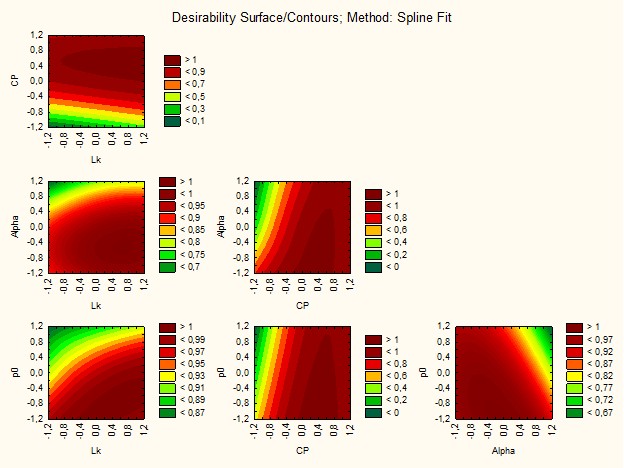
\includegraphics[width=1\textwidth]{P1M2_GV_makespan_DSC}
\end{figure}

\begin{table}[H]
\caption{Effect Estimates; Var.:Tempo; R-sqr=0,97945; Adj:0,96576; 4 3-level factors, 1 Blocks, 81 Runs; MS Residual=10,33885; DV: Tempo. Modelo 3, problema de \textit{makespan}}
\label{tab:P1M2_GV_tempo}
\hspace*{-1.2cm} % shift left (tune the value)
\resizebox{1.2\textwidth}{!}{% scale relative to textwidth
\begin{tabular}{
>{\columncolor[HTML]{FFFFFF}}l 
>{\columncolor[HTML]{FFFFFF}}l 
>{\columncolor[HTML]{FFFFFF}}l 
>{\columncolor[HTML]{FFFFFF}}l 
>{\columncolor[HTML]{FFFFFF}}l 
>{\columncolor[HTML]{FFFFFF}}l 
>{\columncolor[HTML]{FFFFFF}}l 
>{\columncolor[HTML]{FFFFFF}}l 
>{\columncolor[HTML]{FFFFFF}}l 
>{\columncolor[HTML]{FFFFFF}}l 
>{\columncolor[HTML]{FFFFFF}}l }
{\color[HTML]{000000} Factors}        & \cellcolor[HTML]{FFFFFF}{\color[HTML]{000000} Effect} & \cellcolor[HTML]{FFFFFF}{\color[HTML]{000000} Std.Err} & \cellcolor[HTML]{FFFFFF}{\color[HTML]{000000} t(48)} & \cellcolor[HTML]{FFFFFF}{\color[HTML]{000000} p} & \cellcolor[HTML]{FFFFFF}{\color[HTML]{000000} -95\% Cnf.Limt} & \cellcolor[HTML]{FFFFFF}{\color[HTML]{000000} +95\% Cnf.Limt} & \cellcolor[HTML]{FFFFFF}{\color[HTML]{000000} Coeff.} & \cellcolor[HTML]{FFFFFF}{\color[HTML]{000000} Std.Err.Coeff} & \cellcolor[HTML]{FFFFFF}{\color[HTML]{000000} -95\% Cnf.Limt} & \cellcolor[HTML]{FFFFFF}{\color[HTML]{000000} +95\% Cnf.Limt} \\
{\color[HTML]{000000} Mean/Interc.}   & {\color[HTML]{FE0000} 18,67782}                       & {\color[HTML]{FE0000} 0,357268}                        & {\color[HTML]{FE0000} 52,27963}                      & {\color[HTML]{FE0000} 0,000000}                  & {\color[HTML]{FE0000} 17,95948}                               & {\color[HTML]{FE0000} 19,39615}                               & {\color[HTML]{FE0000} 18,67782}                       & {\color[HTML]{FE0000} 0,357268}                              & {\color[HTML]{FE0000} 17,95948}                               & {\color[HTML]{FE0000} 19,39615}                               \\
{\color[HTML]{000000} (1)Lk      (L)} & {\color[HTML]{FE0000} 23,68873}                       & {\color[HTML]{FE0000} 0,875123}                        & {\color[HTML]{FE0000} 27,06902}                      & {\color[HTML]{FE0000} 0,000000}                  & {\color[HTML]{FE0000} 21,92917}                               & {\color[HTML]{FE0000} 25,44828}                               & {\color[HTML]{FE0000} 11,84436}                       & {\color[HTML]{FE0000} 0,437562}                              & {\color[HTML]{FE0000} 10,96459}                               & {\color[HTML]{FE0000} 12,72414}                               \\
{\color[HTML]{000000} Lk      (Q)}    & {\color[HTML]{000000} 0,10397}                        & {\color[HTML]{000000} 0,757879}                        & {\color[HTML]{000000} 0,13718}                       & {\color[HTML]{000000} 0,891460}                  & {\color[HTML]{000000} -1,41985}                               & {\color[HTML]{000000} 1,62779}                                & {\color[HTML]{000000} 0,05198}                        & {\color[HTML]{000000} 0,378939}                              & {\color[HTML]{000000} -0,70993}                               & {\color[HTML]{000000} 0,81389}                                \\
{\color[HTML]{000000} (2)CP      (L)} & {\color[HTML]{FE0000} 28,05016}                       & {\color[HTML]{FE0000} 0,875123}                        & {\color[HTML]{FE0000} 32,05281}                      & {\color[HTML]{FE0000} 0,000000}                  & {\color[HTML]{FE0000} 26,29061}                               & {\color[HTML]{FE0000} 29,80971}                               & {\color[HTML]{FE0000} 14,02508}                       & {\color[HTML]{FE0000} 0,437562}                              & {\color[HTML]{FE0000} 13,14530}                               & {\color[HTML]{FE0000} 14,90486}                               \\
{\color[HTML]{000000} CP      (Q)}    & {\color[HTML]{FE0000} 2,21749}                        & {\color[HTML]{FE0000} 0,757879}                        & {\color[HTML]{FE0000} 2,92592}                       & {\color[HTML]{FE0000} 0,005233}                  & {\color[HTML]{FE0000} 0,69368}                                & {\color[HTML]{FE0000} 3,74131}                                & {\color[HTML]{FE0000} 1,10875}                        & {\color[HTML]{FE0000} 0,378939}                              & {\color[HTML]{FE0000} 0,34684}                                & {\color[HTML]{FE0000} 1,87066}                                \\
{\color[HTML]{000000} (3)Alpha   (L)} & {\color[HTML]{FE0000} 8,28376}                        & {\color[HTML]{FE0000} 0,875123}                        & {\color[HTML]{FE0000} 9,46582}                       & {\color[HTML]{FE0000} 0,000000}                  & {\color[HTML]{FE0000} 6,52421}                                & {\color[HTML]{FE0000} 10,04331}                               & {\color[HTML]{FE0000} 4,14188}                        & {\color[HTML]{FE0000} 0,437562}                              & {\color[HTML]{FE0000} 3,26210}                                & {\color[HTML]{FE0000} 5,02166}                                \\
{\color[HTML]{000000} Alpha   (Q)}    & {\color[HTML]{FE0000} -3,11745}                       & {\color[HTML]{FE0000} 0,757879}                        & {\color[HTML]{FE0000} -4,11338}                      & {\color[HTML]{FE0000} 0,000152}                  & {\color[HTML]{FE0000} -4,64127}                               & {\color[HTML]{FE0000} -1,59363}                               & {\color[HTML]{FE0000} -1,55872}                       & {\color[HTML]{FE0000} 0,378939}                              & {\color[HTML]{FE0000} -2,32063}                               & {\color[HTML]{FE0000} -0,79682}                               \\
{\color[HTML]{000000} (4)p0      (L)} & {\color[HTML]{FE0000} 2,35684}                        & {\color[HTML]{FE0000} 0,875123}                        & {\color[HTML]{FE0000} 2,69316}                       & {\color[HTML]{FE0000} 0,009720}                  & {\color[HTML]{FE0000} 0,59729}                                & {\color[HTML]{FE0000} 4,11640}                                & {\color[HTML]{FE0000} 1,17842}                        & {\color[HTML]{FE0000} 0,437562}                              & {\color[HTML]{FE0000} 0,29865}                                & {\color[HTML]{FE0000} 2,05820}                                \\
{\color[HTML]{000000} p0      (Q)}    & {\color[HTML]{000000} -0,32421}                       & {\color[HTML]{000000} 0,757879}                        & {\color[HTML]{000000} -0,42778}                      & {\color[HTML]{000000} 0,670724}                  & {\color[HTML]{000000} -1,84802}                               & {\color[HTML]{000000} 1,19961}                                & {\color[HTML]{000000} -0,16210}                       & {\color[HTML]{000000} 0,378939}                              & {\color[HTML]{000000} -0,92401}                               & {\color[HTML]{000000} 0,59981}                                \\
{\color[HTML]{000000} 1L by 2L}       & {\color[HTML]{FE0000} 17,15184}                       & {\color[HTML]{FE0000} 1,071803}                        & {\color[HTML]{FE0000} 16,00280}                      & {\color[HTML]{FE0000} 0,000000}                  & {\color[HTML]{FE0000} 14,99684}                               & {\color[HTML]{FE0000} 19,30685}                               & {\color[HTML]{FE0000} 8,57592}                        & {\color[HTML]{FE0000} 0,535901}                              & {\color[HTML]{FE0000} 7,49842}                                & {\color[HTML]{FE0000} 9,65342}                                \\
{\color[HTML]{000000} 1L by 2Q}       & {\color[HTML]{FE0000} 1,94505}                        & {\color[HTML]{FE0000} 0,928208}                        & {\color[HTML]{FE0000} 2,09549}                       & {\color[HTML]{FE0000} 0,041427}                  & {\color[HTML]{FE0000} 0,07876}                                & {\color[HTML]{FE0000} 3,81134}                                & {\color[HTML]{FE0000} 0,97252}                        & {\color[HTML]{FE0000} 0,464104}                              & {\color[HTML]{FE0000} 0,03938}                                & {\color[HTML]{FE0000} 1,90567}                                \\
{\color[HTML]{000000} 1Q by 2L}       & {\color[HTML]{000000} 0,34062}                        & {\color[HTML]{000000} 0,928208}                        & {\color[HTML]{000000} 0,36697}                       & {\color[HTML]{000000} 0,715257}                  & {\color[HTML]{000000} -1,52567}                               & {\color[HTML]{000000} 2,20691}                                & {\color[HTML]{000000} 0,17031}                        & {\color[HTML]{000000} 0,464104}                              & {\color[HTML]{000000} -0,76283}                               & {\color[HTML]{000000} 1,10345}                                \\
{\color[HTML]{000000} 1Q by 2Q}       & {\color[HTML]{000000} -0,27891}                       & {\color[HTML]{000000} 0,803852}                        & {\color[HTML]{000000} -0,34697}                      & {\color[HTML]{000000} 0,730133}                  & {\color[HTML]{000000} -1,89516}                               & {\color[HTML]{000000} 1,33734}                                & {\color[HTML]{000000} -0,13945}                       & {\color[HTML]{000000} 0,401926}                              & {\color[HTML]{000000} -0,94758}                               & {\color[HTML]{000000} 0,66867}                                \\
{\color[HTML]{000000} 1L by 3L}       & {\color[HTML]{FE0000} 6,60764}                        & {\color[HTML]{FE0000} 1,071803}                        & {\color[HTML]{FE0000} 6,16497}                       & {\color[HTML]{FE0000} 0,000000}                  & {\color[HTML]{FE0000} 4,45263}                                & {\color[HTML]{FE0000} 8,76264}                                & {\color[HTML]{FE0000} 3,30382}                        & {\color[HTML]{FE0000} 0,535901}                              & {\color[HTML]{FE0000} 2,22632}                                & {\color[HTML]{FE0000} 4,38132}                                \\
{\color[HTML]{000000} 1L by 3Q}       & {\color[HTML]{FE0000} -2,15015}                       & {\color[HTML]{FE0000} 0,928208}                        & {\color[HTML]{FE0000} -2,31645}                      & {\color[HTML]{FE0000} 0,024848}                  & {\color[HTML]{FE0000} -4,01644}                               & {\color[HTML]{FE0000} -0,28386}                               & {\color[HTML]{FE0000} -1,07508}                       & {\color[HTML]{FE0000} 0,464104}                              & {\color[HTML]{FE0000} -2,00822}                               & {\color[HTML]{FE0000} -0,14193}                               \\
{\color[HTML]{000000} 1Q by 3L}       & {\color[HTML]{000000} -0,57409}                       & {\color[HTML]{000000} 0,928208}                        & {\color[HTML]{000000} -0,61850}                      & {\color[HTML]{000000} 0,539172}                  & {\color[HTML]{000000} -2,44038}                               & {\color[HTML]{000000} 1,29219}                                & {\color[HTML]{000000} -0,28705}                       & {\color[HTML]{000000} 0,464104}                              & {\color[HTML]{000000} -1,22019}                               & {\color[HTML]{000000} 0,64610}                                \\
{\color[HTML]{000000} 1Q by 3Q}       & {\color[HTML]{000000} -0,38687}                       & {\color[HTML]{000000} 0,803852}                        & {\color[HTML]{000000} -0,48127}                      & {\color[HTML]{000000} 0,632512}                  & {\color[HTML]{000000} -2,00312}                               & {\color[HTML]{000000} 1,22938}                                & {\color[HTML]{000000} -0,19343}                       & {\color[HTML]{000000} 0,401926}                              & {\color[HTML]{000000} -1,00156}                               & {\color[HTML]{000000} 0,61469}                                \\
{\color[HTML]{000000} 1L by 4L}       & {\color[HTML]{000000} 1,69692}                        & {\color[HTML]{000000} 1,071803}                        & {\color[HTML]{000000} 1,58324}                       & {\color[HTML]{000000} 0,119934}                  & {\color[HTML]{000000} -0,45808}                               & {\color[HTML]{000000} 3,85193}                                & {\color[HTML]{000000} 0,84846}                        & {\color[HTML]{000000} 0,535901}                              & {\color[HTML]{000000} -0,22904}                               & {\color[HTML]{000000} 1,92596}                                \\
{\color[HTML]{000000} 1L by 4Q}       & {\color[HTML]{000000} -0,30746}                       & {\color[HTML]{000000} 0,928208}                        & {\color[HTML]{000000} -0,33124}                      & {\color[HTML]{000000} 0,741905}                  & {\color[HTML]{000000} -2,17375}                               & {\color[HTML]{000000} 1,55883}                                & {\color[HTML]{000000} -0,15373}                       & {\color[HTML]{000000} 0,464104}                              & {\color[HTML]{000000} -1,08687}                               & {\color[HTML]{000000} 0,77941}                                \\
{\color[HTML]{000000} 1Q by 4L}       & {\color[HTML]{000000} 0,10229}                        & {\color[HTML]{000000} 0,928208}                        & {\color[HTML]{000000} 0,11020}                       & {\color[HTML]{000000} 0,912713}                  & {\color[HTML]{000000} -1,76400}                               & {\color[HTML]{000000} 1,96857}                                & {\color[HTML]{000000} 0,05114}                        & {\color[HTML]{000000} 0,464104}                              & {\color[HTML]{000000} -0,88200}                               & {\color[HTML]{000000} 0,98429}                                \\
{\color[HTML]{000000} 1Q by 4Q}       & {\color[HTML]{000000} -0,01460}                       & {\color[HTML]{000000} 0,803852}                        & {\color[HTML]{000000} -0,01816}                      & {\color[HTML]{000000} 0,985586}                  & {\color[HTML]{000000} -1,63085}                               & {\color[HTML]{000000} 1,60165}                                & {\color[HTML]{000000} -0,00730}                       & {\color[HTML]{000000} 0,401926}                              & {\color[HTML]{000000} -0,81543}                               & {\color[HTML]{000000} 0,80083}                                \\
{\color[HTML]{000000} 2L by 3L}       & {\color[HTML]{FE0000} 9,26165}                        & {\color[HTML]{FE0000} 1,071803}                        & {\color[HTML]{FE0000} 8,64119}                       & {\color[HTML]{FE0000} 0,000000}                  & {\color[HTML]{FE0000} 7,10665}                                & {\color[HTML]{FE0000} 11,41665}                               & {\color[HTML]{FE0000} 4,63082}                        & {\color[HTML]{FE0000} 0,535901}                              & {\color[HTML]{FE0000} 3,55332}                                & {\color[HTML]{FE0000} 5,70833}                                \\
{\color[HTML]{000000} 2L by 3Q}       & {\color[HTML]{FE0000} -3,39010}                       & {\color[HTML]{FE0000} 0,928208}                        & {\color[HTML]{FE0000} -3,65231}                      & {\color[HTML]{FE0000} 0,000642}                  & {\color[HTML]{FE0000} -5,25639}                               & {\color[HTML]{FE0000} -1,52381}                               & {\color[HTML]{FE0000} -1,69505}                       & {\color[HTML]{FE0000} 0,464104}                              & {\color[HTML]{FE0000} -2,62819}                               & {\color[HTML]{FE0000} -0,76191}                               \\
{\color[HTML]{000000} 2Q by 3L}       & {\color[HTML]{000000} 0,71289}                        & {\color[HTML]{000000} 0,928208}                        & {\color[HTML]{000000} 0,76803}                       & {\color[HTML]{000000} 0,446234}                  & {\color[HTML]{000000} -1,15340}                               & {\color[HTML]{000000} 2,57918}                                & {\color[HTML]{000000} 0,35644}                        & {\color[HTML]{000000} 0,464104}                              & {\color[HTML]{000000} -0,57670}                               & {\color[HTML]{000000} 1,28959}                                \\
{\color[HTML]{000000} 2Q by 3Q}       & {\color[HTML]{000000} 0,30248}                        & {\color[HTML]{000000} 0,803852}                        & {\color[HTML]{000000} 0,37629}                       & {\color[HTML]{000000} 0,708356}                  & {\color[HTML]{000000} -1,31377}                               & {\color[HTML]{000000} 1,91874}                                & {\color[HTML]{000000} 0,15124}                        & {\color[HTML]{000000} 0,401926}                              & {\color[HTML]{000000} -0,65688}                               & {\color[HTML]{000000} 0,95937}                                \\
{\color[HTML]{000000} 2L by 4L}       & {\color[HTML]{FE0000} 2,67906}                        & {\color[HTML]{FE0000} 1,071803}                        & {\color[HTML]{FE0000} 2,49958}                       & {\color[HTML]{FE0000} 0,015906}                  & {\color[HTML]{FE0000} 0,52406}                                & {\color[HTML]{FE0000} 4,83407}                                & {\color[HTML]{FE0000} 1,33953}                        & {\color[HTML]{FE0000} 0,535901}                              & {\color[HTML]{FE0000} 0,26203}                                & {\color[HTML]{FE0000} 2,41703}                                \\
{\color[HTML]{000000} 2L by 4Q}       & {\color[HTML]{000000} -0,68407}                       & {\color[HTML]{000000} 0,928208}                        & {\color[HTML]{000000} -0,73698}                      & {\color[HTML]{000000} 0,464724}                  & {\color[HTML]{000000} -2,55036}                               & {\color[HTML]{000000} 1,18222}                                & {\color[HTML]{000000} -0,34203}                       & {\color[HTML]{000000} 0,464104}                              & {\color[HTML]{000000} -1,27518}                               & {\color[HTML]{000000} 0,59111}                                \\
{\color[HTML]{000000} 2Q by 4L}       & {\color[HTML]{000000} -0,22473}                       & {\color[HTML]{000000} 0,928208}                        & {\color[HTML]{000000} -0,24211}                      & {\color[HTML]{000000} 0,809723}                  & {\color[HTML]{000000} -2,09102}                               & {\color[HTML]{000000} 1,64155}                                & {\color[HTML]{000000} -0,11237}                       & {\color[HTML]{000000} 0,464104}                              & {\color[HTML]{000000} -1,04551}                               & {\color[HTML]{000000} 0,82078}                                \\
{\color[HTML]{000000} 2Q by 4Q}       & {\color[HTML]{000000} 0,39673}                        & {\color[HTML]{000000} 0,803852}                        & {\color[HTML]{000000} 0,49354}                       & {\color[HTML]{000000} 0,623881}                  & {\color[HTML]{000000} -1,21952}                               & {\color[HTML]{000000} 2,01299}                                & {\color[HTML]{000000} 0,19837}                        & {\color[HTML]{000000} 0,401926}                              & {\color[HTML]{000000} -0,60976}                               & {\color[HTML]{000000} 1,00649}                                \\
{\color[HTML]{000000} 3L by 4L}       & {\color[HTML]{000000} 1,37885}                        & {\color[HTML]{000000} 1,071803}                        & {\color[HTML]{000000} 1,28648}                       & {\color[HTML]{000000} 0,204446}                  & {\color[HTML]{000000} -0,77615}                               & {\color[HTML]{000000} 3,53386}                                & {\color[HTML]{000000} 0,68943}                        & {\color[HTML]{000000} 0,535901}                              & {\color[HTML]{000000} -0,38807}                               & {\color[HTML]{000000} 1,76693}                                \\
{\color[HTML]{000000} 3L by 4Q}       & {\color[HTML]{000000} 0,29705}                        & {\color[HTML]{000000} 0,928208}                        & {\color[HTML]{000000} 0,32002}                       & {\color[HTML]{000000} 0,750341}                  & {\color[HTML]{000000} -1,56924}                               & {\color[HTML]{000000} 2,16333}                                & {\color[HTML]{000000} 0,14852}                        & {\color[HTML]{000000} 0,464104}                              & {\color[HTML]{000000} -0,78462}                               & {\color[HTML]{000000} 1,08167}                                \\
{\color[HTML]{000000} 3Q by 4L}       & {\color[HTML]{000000} -0,68893}                       & {\color[HTML]{000000} 0,928208}                        & {\color[HTML]{000000} -0,74222}                      & {\color[HTML]{000000} 0,461572}                  & {\color[HTML]{000000} -2,55522}                               & {\color[HTML]{000000} 1,17735}                                & {\color[HTML]{000000} -0,34447}                       & {\color[HTML]{000000} 0,464104}                              & {\color[HTML]{000000} -1,27761}                               & {\color[HTML]{000000} 0,58868}                                \\
{\color[HTML]{000000} 3Q by 4Q}       & {\color[HTML]{000000} -0,32955}                       & {\color[HTML]{000000} 0,803852}                        & {\color[HTML]{000000} -0,40996}                      & {\color[HTML]{000000} 0,683656}                  & {\color[HTML]{000000} -1,94580}                               & {\color[HTML]{000000} 1,28670}                                & {\color[HTML]{000000} -0,16478}                       & {\color[HTML]{000000} 0,401926}                              & {\color[HTML]{000000} -0,97290}                               & {\color[HTML]{000000} 0,64335}                               
\end{tabular}
}
\end{table}

\begin{figure}[H]
\caption{Gráfico de contorno das quatro variáveis relevantes ($L_{k}$, $CP$, $\alpha$, $p_{0}$), relativamente ao tempo, do Modelo 3 do problema de \textit{makespan}}
\centering
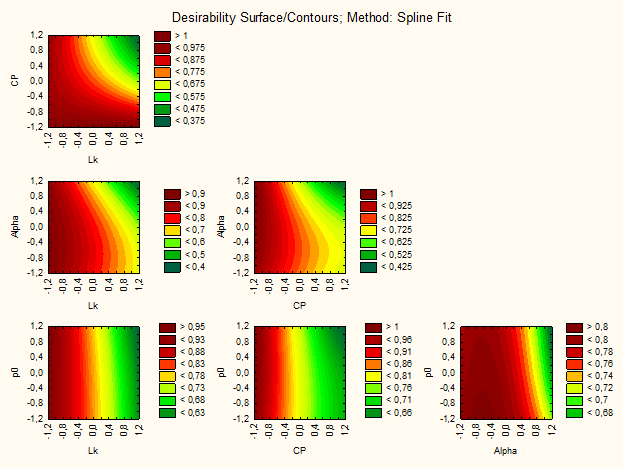
\includegraphics[width=1\textwidth]{P1M2_GV_tempo_DSC}
\end{figure}

\section{Problema do número de trabalhos}

\begin{table}[H]
\caption{Effect Estimates; Var.:Trabalhos; R-sqr=,89764; Adj:,87098; 5 3-level factors, 1 Blocks, 243 Runs; MS Residual=4,373206; DV: Trabalhos. Modelo 1, problema do número de trabalhos}
\label{tab:P2M1_NNGV_trabalhos}
\hspace*{-1.2cm} % shift left (tune the value)
\resizebox{1.2\textwidth}{!}{% scale relative to textwidth
\begin{tabular}{lllllllllll}
Factors               & Effect                          & Std.Err                         & t(192)                          & p                               & -95,\%Cnf.Limt                  & +95,\%Cnf.Limt                  & Coeff.                          & Std.Err.Coeff.                  & -95,\%Cnf.Limt                  & +95,\%Cnf.Limt                  \\
\rowcolor[HTML]{FFFFFF} 
Mean/Interc.   & {\color[HTML]{FF0000} -28,6741} & {\color[HTML]{FF0000} 0,134152} & {\color[HTML]{FF0000} -213,743} & {\color[HTML]{FF0000} 0,000000} & {\color[HTML]{FF0000} -28,9387} & {\color[HTML]{FF0000} -28,4095} & {\color[HTML]{FF0000} -28,6741} & {\color[HTML]{FF0000} 0,134152} & {\color[HTML]{FF0000} -28,9387} & {\color[HTML]{FF0000} -28,4095} \\
\rowcolor[HTML]{FFFFFF} 
(1)Lk      (L) & {\color[HTML]{FF0000} -0,6963}  & {\color[HTML]{FF0000} 0,328604} & {\color[HTML]{FF0000} -2,119}   & {\color[HTML]{FF0000} 0,035380} & {\color[HTML]{FF0000} -1,3444}  & {\color[HTML]{FF0000} -0,0482}  & {\color[HTML]{FF0000} -0,3481}  & {\color[HTML]{FF0000} 0,164302} & {\color[HTML]{FF0000} -0,6722}  & {\color[HTML]{FF0000} -0,0241}  \\
\rowcolor[HTML]{FFFFFF} 
Lk      (Q)    & -0,1852                         & 0,284579                        & -0,651                          & 0,515997                        & -0,7465                         & 0,3761                          & -0,0926                         & 0,142290                        & -0,3732                         & 0,1881                          \\
\rowcolor[HTML]{FFFFFF} 
(2)CP      (L) & {\color[HTML]{FF0000} -6,6815}  & {\color[HTML]{FF0000} 0,328604} & {\color[HTML]{FF0000} -20,333}  & {\color[HTML]{FF0000} 0,000000} & {\color[HTML]{FF0000} -7,3296}  & {\color[HTML]{FF0000} -6,0333}  & {\color[HTML]{FF0000} -3,3407}  & {\color[HTML]{FF0000} 0,164302} & {\color[HTML]{FF0000} -3,6648}  & {\color[HTML]{FF0000} -3,0167}  \\
\rowcolor[HTML]{FFFFFF} 
CP      (Q)    & {\color[HTML]{FF0000} -0,6630}  & {\color[HTML]{FF0000} 0,284579} & {\color[HTML]{FF0000} -2,330}   & {\color[HTML]{FF0000} 0,020866} & {\color[HTML]{FF0000} -1,2243}  & {\color[HTML]{FF0000} -0,1017}  & {\color[HTML]{FF0000} -0,3315}  & {\color[HTML]{FF0000} 0,142290} & {\color[HTML]{FF0000} -0,6121}  & {\color[HTML]{FF0000} -0,0508}  \\
\rowcolor[HTML]{FFFFFF} 
(3)Alpha   (L) & {\color[HTML]{FF0000} 8,2383}   & {\color[HTML]{FF0000} 0,328604} & {\color[HTML]{FF0000} 25,071}   & {\color[HTML]{FF0000} 0,000000} & {\color[HTML]{FF0000} 7,5901}   & {\color[HTML]{FF0000} 8,8864}   & {\color[HTML]{FF0000} 4,1191}   & {\color[HTML]{FF0000} 0,164302} & {\color[HTML]{FF0000} 3,7951}   & {\color[HTML]{FF0000} 4,4432}   \\
\rowcolor[HTML]{FFFFFF} 
Alpha   (Q)    & {\color[HTML]{FF0000} -3,1907}  & {\color[HTML]{FF0000} 0,284579} & {\color[HTML]{FF0000} -11,212}  & {\color[HTML]{FF0000} 0,000000} & {\color[HTML]{FF0000} -3,7520}  & {\color[HTML]{FF0000} -2,6294}  & {\color[HTML]{FF0000} -1,5954}  & {\color[HTML]{FF0000} 0,142290} & {\color[HTML]{FF0000} -1,8760}  & {\color[HTML]{FF0000} -1,3147}  \\
\rowcolor[HTML]{FFFFFF} 
(4)P       (L) & {\color[HTML]{FF0000} 2,4815}   & {\color[HTML]{FF0000} 0,328604} & {\color[HTML]{FF0000} 7,552}    & {\color[HTML]{FF0000} 0,000000} & {\color[HTML]{FF0000} 1,8333}   & {\color[HTML]{FF0000} 3,1296}   & {\color[HTML]{FF0000} 1,2407}   & {\color[HTML]{FF0000} 0,164302} & {\color[HTML]{FF0000} 0,9167}   & {\color[HTML]{FF0000} 1,5648}   \\
\rowcolor[HTML]{FFFFFF} 
P       (Q)    & 0,2815                          & 0,284579                        & 0,989                           & 0,323852                        & -0,2798                         & 0,8428                          & 0,1407                          & 0,142290                        & -0,1399                         & 0,4214                          \\
\rowcolor[HTML]{FFFFFF} 
(5)p0      (L) & {\color[HTML]{FF0000} 1,3679}   & {\color[HTML]{FF0000} 0,328604} & {\color[HTML]{FF0000} 4,163}    & {\color[HTML]{FF0000} 0,000047} & {\color[HTML]{FF0000} 0,7198}   & {\color[HTML]{FF0000} 2,0160}   & {\color[HTML]{FF0000} 0,6840}   & {\color[HTML]{FF0000} 0,164302} & {\color[HTML]{FF0000} 0,3599}   & {\color[HTML]{FF0000} 1,0080}   \\
\rowcolor[HTML]{FFFFFF} 
p0      (Q)    & 0,0222                          & 0,284579                        & 0,078                           & 0,937839                        & -0,5391                         & 0,5835                          & 0,0111                          & 0,142290                        & -0,2695                         & 0,2918                          \\
\rowcolor[HTML]{FFFFFF} 
1L by 2L       & -0,3278                         & 0,402456                        & -0,814                          & 0,416399                        & -1,1216                         & 0,4660                          & -0,1639                         & 0,201228                        & -0,5608                         & 0,2330                          \\
\rowcolor[HTML]{FFFFFF} 
1L by 2Q       & -0,0250                         & 0,348537                        & -0,072                          & 0,942893                        & -0,7125                         & 0,6625                          & -0,0125                         & 0,174268                        & -0,3562                         & 0,3312                          \\
\rowcolor[HTML]{FFFFFF} 
1Q by 2L       & 0,0361                          & 0,348537                        & 0,104                           & 0,917589                        & -0,6513                         & 0,7236                          & 0,0181                          & 0,174268                        & -0,3257                         & 0,3618                          \\
\rowcolor[HTML]{FFFFFF} 
1Q by 2Q       & -0,0347                         & 0,301842                        & -0,115                          & 0,908538                        & -0,6301                         & 0,5606                          & -0,0174                         & 0,150921                        & -0,3150                         & 0,2803                          \\
\rowcolor[HTML]{FFFFFF} 
1L by 3L       & 0,2241                          & 0,402456                        & 0,557                           & 0,578335                        & -0,5697                         & 1,0179                          & 0,1120                          & 0,201228                        & -0,2849                         & 0,5089                          \\
\rowcolor[HTML]{FFFFFF} 
1L by 3Q       & 0,2861                          & 0,348537                        & 0,821                           & 0,412726                        & -0,4013                         & 0,9736                          & 0,1431                          & 0,174268                        & -0,2007                         & 0,4868                          \\
\rowcolor[HTML]{FFFFFF} 
1Q by 3L       & 0,0546                          & 0,348537                        & 0,157                           & 0,875615                        & -0,6328                         & 0,7421                          & 0,0273                          & 0,174268                        & -0,3164                         & 0,3710                          \\
\rowcolor[HTML]{FFFFFF} 
1Q by 3Q       & -0,0431                         & 0,301842                        & -0,143                          & 0,886722                        & -0,6384                         & 0,5523                          & -0,0215                         & 0,150921                        & -0,3192                         & 0,2761                          \\
\rowcolor[HTML]{FFFFFF} 
1L by 4L       & 0,2889                          & 0,402456                        & 0,718                           & 0,473744                        & -0,5049                         & 1,0827                          & 0,1444                          & 0,201228                        & -0,2525                         & 0,5413                          \\
\rowcolor[HTML]{FFFFFF} 
1L by 4Q       & -0,1444                         & 0,348537                        & -0,414                          & 0,679021                        & -0,8319                         & 0,5430                          & -0,0722                         & 0,174268                        & -0,4159                         & 0,2715                          \\
\rowcolor[HTML]{FFFFFF} 
1Q by 4L       & -0,0389                         & 0,348537                        & -0,112                          & 0,911275                        & -0,7263                         & 0,6486                          & -0,0194                         & 0,174268                        & -0,3632                         & 0,3243                          \\
\rowcolor[HTML]{FFFFFF} 
1Q by 4Q       & 0,1694                          & 0,301842                        & 0,561                           & 0,575201                        & -0,4259                         & 0,7648                          & 0,0847                          & 0,150921                        & -0,2130                         & 0,3824                          \\
\rowcolor[HTML]{FFFFFF} 
1L by 5L       & 0,2907                          & 0,402456                        & 0,722                           & 0,470917                        & -0,5031                         & 1,0845                          & 0,1454                          & 0,201228                        & -0,2515                         & 0,5423                          \\
\rowcolor[HTML]{FFFFFF} 
1L by 5Q       & -0,1361                         & 0,348537                        & -0,391                          & 0,696584                        & -0,8236                         & 0,5513                          & -0,0681                         & 0,174268                        & -0,4118                         & 0,2757                          \\
\rowcolor[HTML]{FFFFFF} 
1Q by 5L       & 0,1102                          & 0,348537                        & 0,316                           & 0,752242                        & -0,5773                         & 0,7976                          & 0,0551                          & 0,174268                        & -0,2886                         & 0,3988                          \\
\rowcolor[HTML]{FFFFFF} 
1Q by 5Q       & 0,2514                          & 0,301842                        & 0,833                           & 0,405964                        & -0,3440                         & 0,8467                          & 0,1257                          & 0,150921                        & -0,1720                         & 0,4234                          \\
\rowcolor[HTML]{FFFFFF} 
2L by 3L       & {\color[HTML]{FF0000} -7,0000}  & {\color[HTML]{FF0000} 0,402456} & {\color[HTML]{FF0000} -17,393}  & {\color[HTML]{FF0000} 0,000000} & {\color[HTML]{FF0000} -7,7938}  & {\color[HTML]{FF0000} -6,2062}  & {\color[HTML]{FF0000} -3,5000}  & {\color[HTML]{FF0000} 0,201228} & {\color[HTML]{FF0000} -3,8969}  & {\color[HTML]{FF0000} -3,1031}  \\
\rowcolor[HTML]{FFFFFF} 
2L by 3Q       & {\color[HTML]{FF0000} 2,0278}   & {\color[HTML]{FF0000} 0,348537} & {\color[HTML]{FF0000} 5,818}    & {\color[HTML]{FF0000} 0,000000} & {\color[HTML]{FF0000} 1,3403}   & {\color[HTML]{FF0000} 2,7152}   & {\color[HTML]{FF0000} 1,0139}   & {\color[HTML]{FF0000} 0,174268} & {\color[HTML]{FF0000} 0,6702}   & {\color[HTML]{FF0000} 1,3576}   \\
\rowcolor[HTML]{FFFFFF} 
2Q by 3L       & 0,0463                          & 0,348537                        & 0,133                           & 0,894467                        & -0,6412                         & 0,7337                          & 0,0231                          & 0,174268                        & -0,3206                         & 0,3669                          \\
\rowcolor[HTML]{FFFFFF} 
2Q by 3Q       & {\color[HTML]{FF0000} -0,7556}  & {\color[HTML]{FF0000} 0,301842} & {\color[HTML]{FF0000} -2,503}   & {\color[HTML]{FF0000} 0,013143} & {\color[HTML]{FF0000} -1,3509}  & {\color[HTML]{FF0000} -0,1602}  & {\color[HTML]{FF0000} -0,3778}  & {\color[HTML]{FF0000} 0,150921} & {\color[HTML]{FF0000} -0,6755}  & {\color[HTML]{FF0000} -0,0801}  \\
\rowcolor[HTML]{FFFFFF} 
2L by 4L       & -0,4500                         & 0,402456                        & -1,118                          & 0,264906                        & -1,2438                         & 0,3438                          & -0,2250                         & 0,201228                        & -0,6219                         & 0,1719                          \\
\rowcolor[HTML]{FFFFFF} 
2L by 4Q       & -0,0194                         & 0,348537                        & -0,056                          & 0,955568                        & -0,7069                         & 0,6680                          & -0,0097                         & 0,174268                        & -0,3534                         & 0,3340                          \\
\rowcolor[HTML]{FFFFFF} 
2Q by 4L       & {\color[HTML]{FF0000} 1,3972}   & {\color[HTML]{FF0000} 0,348537} & {\color[HTML]{FF0000} 4,009}    & {\color[HTML]{FF0000} 0,000087} & {\color[HTML]{FF0000} 0,7098}   & {\color[HTML]{FF0000} 2,0847}   & {\color[HTML]{FF0000} 0,6986}   & {\color[HTML]{FF0000} 0,174268} & {\color[HTML]{FF0000} 0,3549}   & {\color[HTML]{FF0000} 1,0423}   \\
\rowcolor[HTML]{FFFFFF} 
2Q by 4Q       & 0,4403                          & 0,301842                        & 1,459                           & 0,146299                        & -0,1551                         & 1,0356                          & 0,2201                          & 0,150921                        & -0,0775                         & 0,5178                          \\
\rowcolor[HTML]{FFFFFF} 
2L by 5L       & -0,3537                         & 0,402456                        & -0,879                          & 0,380574                        & -1,1475                         & 0,4401                          & -0,1769                         & 0,201228                        & -0,5738                         & 0,2200                          \\
\rowcolor[HTML]{FFFFFF} 
2L by 5Q       & -0,0194                         & 0,348537                        & -0,056                          & 0,955568                        & -0,7069                         & 0,6680                          & -0,0097                         & 0,174268                        & -0,3534                         & 0,3340                          \\
\rowcolor[HTML]{FFFFFF} 
2Q by 5L       & 0,4435                          & 0,348537                        & 1,273                           & 0,204729                        & -0,2439                         & 1,1310                          & 0,2218                          & 0,174268                        & -0,1220                         & 0,5655                          \\
\rowcolor[HTML]{FFFFFF} 
2Q by 5Q       & 0,0597                          & 0,301842                        & 0,198                           & 0,843364                        & -0,5356                         & 0,6551                          & 0,0299                          & 0,150921                        & -0,2678                         & 0,3275                          \\
\rowcolor[HTML]{FFFFFF} 
3L by 4L       & {\color[HTML]{FF0000} 2,6019}   & {\color[HTML]{FF0000} 0,402456} & {\color[HTML]{FF0000} 6,465}    & {\color[HTML]{FF0000} 0,000000} & {\color[HTML]{FF0000} 1,8080}   & {\color[HTML]{FF0000} 3,3957}   & {\color[HTML]{FF0000} 1,3009}   & {\color[HTML]{FF0000} 0,201228} & {\color[HTML]{FF0000} 0,9040}   & {\color[HTML]{FF0000} 1,6978}   \\
\rowcolor[HTML]{FFFFFF} 
3L by 4Q       & 0,3491                          & 0,348537                        & 1,002                           & 0,317826                        & -0,3384                         & 1,0365                          & 0,1745                          & 0,174268                        & -0,1692                         & 0,5183                          \\
\rowcolor[HTML]{FFFFFF} 
3Q by 4L       & -0,3250                         & 0,348537                        & -0,932                          & 0,352265                        & -1,0125                         & 0,3625                          & -0,1625                         & 0,174268                        & -0,5062                         & 0,1812                          \\
\rowcolor[HTML]{FFFFFF} 
3Q by 4Q       & -0,2514                         & 0,301842                        & -0,833                          & 0,405964                        & -0,8467                         & 0,3440                          & -0,1257                         & 0,150921                        & -0,4234                         & 0,1720                          \\
\rowcolor[HTML]{FFFFFF} 
3L by 5L       & {\color[HTML]{FF0000} 1,4185}   & {\color[HTML]{FF0000} 0,402456} & {\color[HTML]{FF0000} 3,525}    & {\color[HTML]{FF0000} 0,000530} & {\color[HTML]{FF0000} 0,6247}   & {\color[HTML]{FF0000} 2,2123}   & {\color[HTML]{FF0000} 0,7093}   & {\color[HTML]{FF0000} 0,201228} & {\color[HTML]{FF0000} 0,3124}   & {\color[HTML]{FF0000} 1,1062}   \\
\rowcolor[HTML]{FFFFFF} 
3L by 5Q       & 0,1074                          & 0,348537                        & 0,308                           & 0,758290                        & -0,5800                         & 0,7949                          & 0,0537                          & 0,174268                        & -0,2900                         & 0,3974                          \\
\rowcolor[HTML]{FFFFFF} 
3Q by 5L       & 0,0185                          & 0,348537                        & 0,053                           & 0,957682                        & -0,6689                         & 0,7060                          & 0,0093                          & 0,174268                        & -0,3345                         & 0,3530                          \\
\rowcolor[HTML]{FFFFFF} 
3Q by 5Q       & -0,0194                         & 0,301842                        & -0,064                          & 0,948703                        & -0,6148                         & 0,5759                          & -0,0097                         & 0,150921                        & -0,3074                         & 0,2880                          \\
\rowcolor[HTML]{FFFFFF} 
4L by 5L       & 0,6593                          & 0,402456                        & 1,638                           & 0,103040                        & -0,1345                         & 1,4531                          & 0,3296                          & 0,201228                        & -0,0673                         & 0,7265                          \\
\rowcolor[HTML]{FFFFFF} 
4L by 5Q       & 0,1722                          & 0,348537                        & 0,494                           & 0,621780                        & -0,5152                         & 0,8597                          & 0,0861                          & 0,174268                        & -0,2576                         & 0,4298                          \\
\rowcolor[HTML]{FFFFFF} 
4Q by 5L       & 0,4574                          & 0,348537                        & 1,312                           & 0,190964                        & -0,2300                         & 1,1449                          & 0,2287                          & 0,174268                        & -0,1150                         & 0,5724                          \\
\rowcolor[HTML]{FFFFFF} 
4Q by 5Q       & 0,0556                          & 0,301842                        & 0,184                           & 0,854164                        & -0,5398                         & 0,6509                          & 0,0278                          & 0,150921                        & -0,2699                         & 0,3255                         
\end{tabular}
}
\end{table}

\begin{figure}[H]
\caption{Gráfico de contorno das cinco variáveis relevantes ($L_{k}$, $CP$, $\alpha$, $P$, $p_{0}$), relativamente ao número de exames, do Modelo 1 do problema do número de trabalhos}
\centering
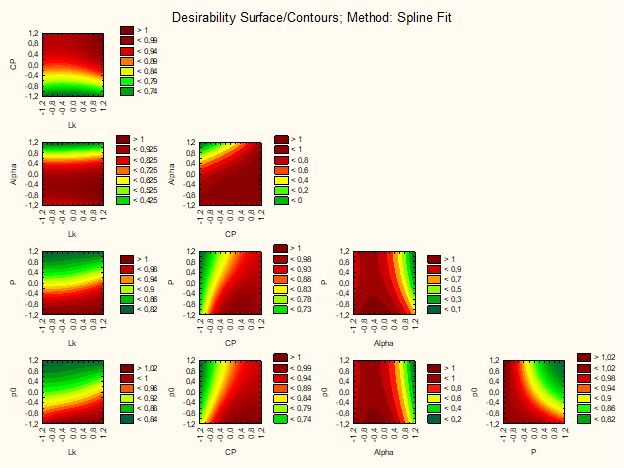
\includegraphics[width=1\textwidth]{P2M1_NNGV_trabalhos_DSC}
\end{figure}

\begin{table}[H]
\caption{Effect Estimates; Var.:Tempo; R-sqr=,96619; Adj:,95739; 5 3-level factors, 1 Blocks, 243 Runs; MS Residual=15,01405; DV: Tempo. Modelo 1, problema do número de trabalhos}
\label{tab:P2M1_NNGV_tempo}
\hspace*{-1.2cm} % shift left (tune the value)
\resizebox{1.2\textwidth}{!}{% scale relative to textwidth
\begin{tabular}{lllllllllll}
Factors               & Effect                          & Std.Err                         & t(192)                          & p                               & -95,\%Cnf.Limt                  & +95,\%Cnf.Limt                  & Coeff.                          & Std.Err.Coeff.                  & -95,\%Cnf.Limt                  & +95,\%Cnf.Limt                  \\
\rowcolor[HTML]{FFFFFF} 
Mean/Interc.   & {\color[HTML]{FF0000} 21,95706} & {\color[HTML]{FF0000} 0,248568} & {\color[HTML]{FF0000} 88,33411} & {\color[HTML]{FF0000} 0,000000} & {\color[HTML]{FF0000} 21,46679} & {\color[HTML]{FF0000} 22,44734} & {\color[HTML]{FF0000} 21,95706} & {\color[HTML]{FF0000} 0,248568} & {\color[HTML]{FF0000} 21,46679} & {\color[HTML]{FF0000} 22,44734} \\
\rowcolor[HTML]{FFFFFF} 
(1)Lk      (L) & {\color[HTML]{FF0000} 27,86540} & {\color[HTML]{FF0000} 0,608866} & {\color[HTML]{FF0000} 45,76610} & {\color[HTML]{FF0000} 0,000000} & {\color[HTML]{FF0000} 26,66448} & {\color[HTML]{FF0000} 29,06633} & {\color[HTML]{FF0000} 13,93270} & {\color[HTML]{FF0000} 0,304433} & {\color[HTML]{FF0000} 13,33224} & {\color[HTML]{FF0000} 14,53316} \\
\rowcolor[HTML]{FFFFFF} 
Lk      (Q)    & {\color[HTML]{181A1B} 0,25520}  & {\color[HTML]{181A1B} 0,527293} & {\color[HTML]{181A1B} 0,48399}  & {\color[HTML]{181A1B} 0,628947} & {\color[HTML]{181A1B} -0,78483} & {\color[HTML]{181A1B} 1,29523}  & {\color[HTML]{181A1B} 0,12760}  & {\color[HTML]{181A1B} 0,263647} & {\color[HTML]{181A1B} -0,39241} & {\color[HTML]{181A1B} 0,64762}  \\
\rowcolor[HTML]{FFFFFF} 
(2)CP      (L) & {\color[HTML]{FF0000} 30,05783} & {\color[HTML]{FF0000} 0,608866} & {\color[HTML]{FF0000} 49,36694} & {\color[HTML]{FF0000} 0,000000} & {\color[HTML]{FF0000} 28,85691} & {\color[HTML]{FF0000} 31,25876} & {\color[HTML]{FF0000} 15,02892} & {\color[HTML]{FF0000} 0,304433} & {\color[HTML]{FF0000} 14,42845} & {\color[HTML]{FF0000} 15,62938} \\
\rowcolor[HTML]{FFFFFF} 
CP      (Q)    & {\color[HTML]{181A1B} -0,60802} & {\color[HTML]{181A1B} 0,527293} & {\color[HTML]{181A1B} -1,15310} & {\color[HTML]{181A1B} 0,250303} & {\color[HTML]{181A1B} -1,64805} & {\color[HTML]{181A1B} 0,43201}  & {\color[HTML]{181A1B} -0,30401} & {\color[HTML]{181A1B} 0,263647} & {\color[HTML]{181A1B} -0,82403} & {\color[HTML]{181A1B} 0,21600}  \\
\rowcolor[HTML]{FFFFFF} 
(3)Alpha   (L) & {\color[HTML]{FF0000} 1,40762}  & {\color[HTML]{FF0000} 0,608866} & {\color[HTML]{FF0000} 2,31187}  & {\color[HTML]{FF0000} 0,021846} & {\color[HTML]{FF0000} 0,20669}  & {\color[HTML]{FF0000} 2,60854}  & {\color[HTML]{FF0000} 0,70381}  & {\color[HTML]{FF0000} 0,304433} & {\color[HTML]{FF0000} 0,10335}  & {\color[HTML]{FF0000} 1,30427}  \\
\rowcolor[HTML]{FFFFFF} 
Alpha   (Q)    & {\color[HTML]{FF0000} 1,09742}  & {\color[HTML]{FF0000} 0,527293} & {\color[HTML]{FF0000} 2,08123}  & {\color[HTML]{FF0000} 0,038740} & {\color[HTML]{FF0000} 0,05739}  & {\color[HTML]{FF0000} 2,13745}  & {\color[HTML]{FF0000} 0,54871}  & {\color[HTML]{FF0000} 0,263647} & {\color[HTML]{FF0000} 0,02869}  & {\color[HTML]{FF0000} 1,06872}  \\
\rowcolor[HTML]{FFFFFF} 
(4)P       (L) & {\color[HTML]{FF0000} -3,04670} & {\color[HTML]{FF0000} 0,608866} & {\color[HTML]{FF0000} -5,00389} & {\color[HTML]{FF0000} 0,000001} & {\color[HTML]{FF0000} -4,24762} & {\color[HTML]{FF0000} -1,84577} & {\color[HTML]{FF0000} -1,52335} & {\color[HTML]{FF0000} 0,304433} & {\color[HTML]{FF0000} -2,12381} & {\color[HTML]{FF0000} -0,92289} \\
\rowcolor[HTML]{FFFFFF} 
P       (Q)    & {\color[HTML]{181A1B} -0,45522} & {\color[HTML]{181A1B} 0,527293} & {\color[HTML]{181A1B} -0,86332} & {\color[HTML]{181A1B} 0,389041} & {\color[HTML]{181A1B} -1,49525} & {\color[HTML]{181A1B} 0,58481}  & {\color[HTML]{181A1B} -0,22761} & {\color[HTML]{181A1B} 0,263647} & {\color[HTML]{181A1B} -0,74763} & {\color[HTML]{181A1B} 0,29241}  \\
\rowcolor[HTML]{FFFFFF} 
(5)p0      (L) & {\color[HTML]{181A1B} -1,10053} & {\color[HTML]{181A1B} 0,608866} & {\color[HTML]{181A1B} -1,80751} & {\color[HTML]{181A1B} 0,072249} & {\color[HTML]{181A1B} -2,30145} & {\color[HTML]{181A1B} 0,10040}  & {\color[HTML]{181A1B} -0,55026} & {\color[HTML]{181A1B} 0,304433} & {\color[HTML]{181A1B} -1,15073} & {\color[HTML]{181A1B} 0,05020}  \\
\rowcolor[HTML]{FFFFFF} 
p0      (Q)    & {\color[HTML]{181A1B} -0,22992} & {\color[HTML]{181A1B} 0,527293} & {\color[HTML]{181A1B} -0,43605} & {\color[HTML]{181A1B} 0,663292} & {\color[HTML]{181A1B} -1,26996} & {\color[HTML]{181A1B} 0,81011}  & {\color[HTML]{181A1B} -0,11496} & {\color[HTML]{181A1B} 0,263647} & {\color[HTML]{181A1B} -0,63498} & {\color[HTML]{181A1B} 0,40505}  \\
\rowcolor[HTML]{FFFFFF} 
1L by 2L       & {\color[HTML]{FF0000} 19,56619} & {\color[HTML]{FF0000} 0,745705} & {\color[HTML]{FF0000} 26,23851} & {\color[HTML]{FF0000} 0,000000} & {\color[HTML]{FF0000} 18,09536} & {\color[HTML]{FF0000} 21,03701} & {\color[HTML]{FF0000} 9,78309}  & {\color[HTML]{FF0000} 0,372853} & {\color[HTML]{FF0000} 9,04768}  & {\color[HTML]{FF0000} 10,51851} \\
\rowcolor[HTML]{FFFFFF} 
1L by 2Q       & {\color[HTML]{181A1B} -0,52683} & {\color[HTML]{181A1B} 0,645799} & {\color[HTML]{181A1B} -0,81578} & {\color[HTML]{181A1B} 0,415634} & {\color[HTML]{181A1B} -1,80061} & {\color[HTML]{181A1B} 0,74694}  & {\color[HTML]{181A1B} -0,26342} & {\color[HTML]{181A1B} 0,322900} & {\color[HTML]{181A1B} -0,90030} & {\color[HTML]{181A1B} 0,37347}  \\
\rowcolor[HTML]{FFFFFF} 
1Q by 2L       & {\color[HTML]{181A1B} 0,14028}  & {\color[HTML]{181A1B} 0,645799} & {\color[HTML]{181A1B} 0,21721}  & {\color[HTML]{181A1B} 0,828272} & {\color[HTML]{181A1B} -1,13350} & {\color[HTML]{181A1B} 1,41405}  & {\color[HTML]{181A1B} 0,07014}  & {\color[HTML]{181A1B} 0,322900} & {\color[HTML]{181A1B} -0,56675} & {\color[HTML]{181A1B} 0,70702}  \\
\rowcolor[HTML]{FFFFFF} 
1Q by 2Q       & {\color[HTML]{181A1B} -0,03114} & {\color[HTML]{181A1B} 0,559279} & {\color[HTML]{181A1B} -0,05569} & {\color[HTML]{181A1B} 0,955650} & {\color[HTML]{181A1B} -1,13426} & {\color[HTML]{181A1B} 1,07198}  & {\color[HTML]{181A1B} -0,01557} & {\color[HTML]{181A1B} 0,279639} & {\color[HTML]{181A1B} -0,56713} & {\color[HTML]{181A1B} 0,53599}  \\
\rowcolor[HTML]{FFFFFF} 
1L by 3L       & {\color[HTML]{181A1B} 1,21568}  & {\color[HTML]{181A1B} 0,745705} & {\color[HTML]{181A1B} 1,63024}  & {\color[HTML]{181A1B} 0,104691} & {\color[HTML]{181A1B} -0,25515} & {\color[HTML]{181A1B} 2,68650}  & {\color[HTML]{181A1B} 0,60784}  & {\color[HTML]{181A1B} 0,372853} & {\color[HTML]{181A1B} -0,12757} & {\color[HTML]{181A1B} 1,34325}  \\
\rowcolor[HTML]{FFFFFF} 
1L by 3Q       & {\color[HTML]{181A1B} 0,77665}  & {\color[HTML]{181A1B} 0,645799} & {\color[HTML]{181A1B} 1,20261}  & {\color[HTML]{181A1B} 0,230608} & {\color[HTML]{181A1B} -0,49713} & {\color[HTML]{181A1B} 2,05042}  & {\color[HTML]{181A1B} 0,38832}  & {\color[HTML]{181A1B} 0,322900} & {\color[HTML]{181A1B} -0,24856} & {\color[HTML]{181A1B} 1,02521}  \\
\rowcolor[HTML]{FFFFFF} 
1Q by 3L       & {\color[HTML]{181A1B} 0,16311}  & {\color[HTML]{181A1B} 0,645799} & {\color[HTML]{181A1B} 0,25257}  & {\color[HTML]{181A1B} 0,800869} & {\color[HTML]{181A1B} -1,11066} & {\color[HTML]{181A1B} 1,43688}  & {\color[HTML]{181A1B} 0,08156}  & {\color[HTML]{181A1B} 0,322900} & {\color[HTML]{181A1B} -0,55533} & {\color[HTML]{181A1B} 0,71844}  \\
\rowcolor[HTML]{FFFFFF} 
1Q by 3Q       & {\color[HTML]{181A1B} -0,41793} & {\color[HTML]{181A1B} 0,559279} & {\color[HTML]{181A1B} -0,74726} & {\color[HTML]{181A1B} 0,455820} & {\color[HTML]{181A1B} -1,52105} & {\color[HTML]{181A1B} 0,68519}  & {\color[HTML]{181A1B} -0,20896} & {\color[HTML]{181A1B} 0,279639} & {\color[HTML]{181A1B} -0,76052} & {\color[HTML]{181A1B} 0,34260}  \\
\rowcolor[HTML]{FFFFFF} 
1L by 4L       & {\color[HTML]{FF0000} -2,33837} & {\color[HTML]{FF0000} 0,745705} & {\color[HTML]{FF0000} -3,13578} & {\color[HTML]{FF0000} 0,001983} & {\color[HTML]{FF0000} -3,80919} & {\color[HTML]{FF0000} -0,86754} & {\color[HTML]{FF0000} -1,16918} & {\color[HTML]{FF0000} 0,372853} & {\color[HTML]{FF0000} -1,90460} & {\color[HTML]{FF0000} -0,43377} \\
\rowcolor[HTML]{FFFFFF} 
1L by 4Q       & {\color[HTML]{181A1B} -0,15421} & {\color[HTML]{181A1B} 0,645799} & {\color[HTML]{181A1B} -0,23880} & {\color[HTML]{181A1B} 0,811519} & {\color[HTML]{181A1B} -1,42799} & {\color[HTML]{181A1B} 1,11956}  & {\color[HTML]{181A1B} -0,07711} & {\color[HTML]{181A1B} 0,322900} & {\color[HTML]{181A1B} -0,71399} & {\color[HTML]{181A1B} 0,55978}  \\
\rowcolor[HTML]{FFFFFF} 
1Q by 4L       & {\color[HTML]{181A1B} 0,14415}  & {\color[HTML]{181A1B} 0,645799} & {\color[HTML]{181A1B} 0,22321}  & {\color[HTML]{181A1B} 0,823609} & {\color[HTML]{181A1B} -1,12962} & {\color[HTML]{181A1B} 1,41792}  & {\color[HTML]{181A1B} 0,07207}  & {\color[HTML]{181A1B} 0,322900} & {\color[HTML]{181A1B} -0,56481} & {\color[HTML]{181A1B} 0,70896}  \\
\rowcolor[HTML]{FFFFFF} 
1Q by 4Q       & {\color[HTML]{181A1B} -0,39463} & {\color[HTML]{181A1B} 0,559279} & {\color[HTML]{181A1B} -0,70561} & {\color[HTML]{181A1B} 0,481289} & {\color[HTML]{181A1B} -1,49775} & {\color[HTML]{181A1B} 0,70849}  & {\color[HTML]{181A1B} -0,19732} & {\color[HTML]{181A1B} 0,279639} & {\color[HTML]{181A1B} -0,74887} & {\color[HTML]{181A1B} 0,35424}  \\
\rowcolor[HTML]{FFFFFF} 
1L by 5L       & {\color[HTML]{181A1B} -1,04255} & {\color[HTML]{181A1B} 0,745705} & {\color[HTML]{181A1B} -1,39807} & {\color[HTML]{181A1B} 0,163706} & {\color[HTML]{181A1B} -2,51337} & {\color[HTML]{181A1B} 0,42828}  & {\color[HTML]{181A1B} -0,52127} & {\color[HTML]{181A1B} 0,372853} & {\color[HTML]{181A1B} -1,25669} & {\color[HTML]{181A1B} 0,21414}  \\
\rowcolor[HTML]{FFFFFF} 
1L by 5Q       & {\color[HTML]{181A1B} 0,28096}  & {\color[HTML]{181A1B} 0,645799} & {\color[HTML]{181A1B} 0,43506}  & {\color[HTML]{181A1B} 0,664010} & {\color[HTML]{181A1B} -0,99281} & {\color[HTML]{181A1B} 1,55473}  & {\color[HTML]{181A1B} 0,14048}  & {\color[HTML]{181A1B} 0,322900} & {\color[HTML]{181A1B} -0,49641} & {\color[HTML]{181A1B} 0,77737}  \\
\rowcolor[HTML]{FFFFFF} 
1Q by 5L       & {\color[HTML]{181A1B} 0,00559}  & {\color[HTML]{181A1B} 0,645799} & {\color[HTML]{181A1B} 0,00866}  & {\color[HTML]{181A1B} 0,993099} & {\color[HTML]{181A1B} -1,26818} & {\color[HTML]{181A1B} 1,27937}  & {\color[HTML]{181A1B} 0,00280}  & {\color[HTML]{181A1B} 0,322900} & {\color[HTML]{181A1B} -0,63409} & {\color[HTML]{181A1B} 0,63968}  \\
\rowcolor[HTML]{FFFFFF} 
1Q by 5Q       & {\color[HTML]{181A1B} -0,44403} & {\color[HTML]{181A1B} 0,559279} & {\color[HTML]{181A1B} -0,79394} & {\color[HTML]{181A1B} 0,428213} & {\color[HTML]{181A1B} -1,54715} & {\color[HTML]{181A1B} 0,65909}  & {\color[HTML]{181A1B} -0,22202} & {\color[HTML]{181A1B} 0,279639} & {\color[HTML]{181A1B} -0,77358} & {\color[HTML]{181A1B} 0,32954}  \\
\rowcolor[HTML]{FFFFFF} 
2L by 3L       & {\color[HTML]{FF0000} 7,77354}  & {\color[HTML]{FF0000} 0,745705} & {\color[HTML]{FF0000} 10,42442} & {\color[HTML]{FF0000} 0,000000} & {\color[HTML]{FF0000} 6,30271}  & {\color[HTML]{FF0000} 9,24436}  & {\color[HTML]{FF0000} 3,88677}  & {\color[HTML]{FF0000} 0,372853} & {\color[HTML]{FF0000} 3,15136}  & {\color[HTML]{FF0000} 4,62218}  \\
\rowcolor[HTML]{FFFFFF} 
2L by 3Q       & {\color[HTML]{FF0000} -2,08694} & {\color[HTML]{FF0000} 0,645799} & {\color[HTML]{FF0000} -3,23157} & {\color[HTML]{FF0000} 0,001449} & {\color[HTML]{FF0000} -3,36072} & {\color[HTML]{FF0000} -0,81317} & {\color[HTML]{FF0000} -1,04347} & {\color[HTML]{FF0000} 0,322900} & {\color[HTML]{FF0000} -1,68036} & {\color[HTML]{FF0000} -0,40659} \\
\rowcolor[HTML]{FFFFFF} 
2Q by 3L       & {\color[HTML]{FF0000} -1,82630} & {\color[HTML]{FF0000} 0,645799} & {\color[HTML]{FF0000} -2,82796} & {\color[HTML]{FF0000} 0,005181} & {\color[HTML]{FF0000} -3,10007} & {\color[HTML]{FF0000} -0,55252} & {\color[HTML]{FF0000} -0,91315} & {\color[HTML]{FF0000} 0,322900} & {\color[HTML]{FF0000} -1,55003} & {\color[HTML]{FF0000} -0,27626} \\
\rowcolor[HTML]{FFFFFF} 
2Q by 3Q       & {\color[HTML]{FF0000} 1,57498}  & {\color[HTML]{FF0000} 0,559279} & {\color[HTML]{FF0000} 2,81608}  & {\color[HTML]{FF0000} 0,005369} & {\color[HTML]{FF0000} 0,47186}  & {\color[HTML]{FF0000} 2,67810}  & {\color[HTML]{FF0000} 0,78749}  & {\color[HTML]{FF0000} 0,279639} & {\color[HTML]{FF0000} 0,23593}  & {\color[HTML]{FF0000} 1,33905}  \\
\rowcolor[HTML]{FFFFFF} 
2L by 4L       & {\color[HTML]{181A1B} -0,78616} & {\color[HTML]{181A1B} 0,745705} & {\color[HTML]{181A1B} -1,05426} & {\color[HTML]{181A1B} 0,293091} & {\color[HTML]{181A1B} -2,25699} & {\color[HTML]{181A1B} 0,68466}  & {\color[HTML]{181A1B} -0,39308} & {\color[HTML]{181A1B} 0,372853} & {\color[HTML]{181A1B} -1,12849} & {\color[HTML]{181A1B} 0,34233}  \\
\rowcolor[HTML]{FFFFFF} 
2L by 4Q       & {\color[HTML]{181A1B} -0,01159} & {\color[HTML]{181A1B} 0,645799} & {\color[HTML]{181A1B} -0,01795} & {\color[HTML]{181A1B} 0,985700} & {\color[HTML]{181A1B} -1,28536} & {\color[HTML]{181A1B} 1,26218}  & {\color[HTML]{181A1B} -0,00580} & {\color[HTML]{181A1B} 0,322900} & {\color[HTML]{181A1B} -0,64268} & {\color[HTML]{181A1B} 0,63109}  \\
\rowcolor[HTML]{FFFFFF} 
2Q by 4L       & {\color[HTML]{FF0000} -1,89371} & {\color[HTML]{FF0000} 0,645799} & {\color[HTML]{FF0000} -2,93235} & {\color[HTML]{FF0000} 0,003773} & {\color[HTML]{FF0000} -3,16748} & {\color[HTML]{FF0000} -0,61993} & {\color[HTML]{FF0000} -0,94685} & {\color[HTML]{FF0000} 0,322900} & {\color[HTML]{FF0000} -1,58374} & {\color[HTML]{FF0000} -0,30997} \\
\rowcolor[HTML]{FFFFFF} 
2Q by 4Q       & {\color[HTML]{181A1B} -0,39480} & {\color[HTML]{181A1B} 0,559279} & {\color[HTML]{181A1B} -0,70591} & {\color[HTML]{181A1B} 0,481098} & {\color[HTML]{181A1B} -1,49792} & {\color[HTML]{181A1B} 0,70832}  & {\color[HTML]{181A1B} -0,19740} & {\color[HTML]{181A1B} 0,279639} & {\color[HTML]{181A1B} -0,74896} & {\color[HTML]{181A1B} 0,35416}  \\
\rowcolor[HTML]{FFFFFF} 
2L by 5L       & {\color[HTML]{181A1B} -0,22339} & {\color[HTML]{181A1B} 0,745705} & {\color[HTML]{181A1B} -0,29957} & {\color[HTML]{181A1B} 0,764827} & {\color[HTML]{181A1B} -1,69422} & {\color[HTML]{181A1B} 1,24743}  & {\color[HTML]{181A1B} -0,11170} & {\color[HTML]{181A1B} 0,372853} & {\color[HTML]{181A1B} -0,84711} & {\color[HTML]{181A1B} 0,62372}  \\
\rowcolor[HTML]{FFFFFF} 
2L by 5Q       & {\color[HTML]{181A1B} -0,16161} & {\color[HTML]{181A1B} 0,645799} & {\color[HTML]{181A1B} -0,25024} & {\color[HTML]{181A1B} 0,802668} & {\color[HTML]{181A1B} -1,43538} & {\color[HTML]{181A1B} 1,11217}  & {\color[HTML]{181A1B} -0,08080} & {\color[HTML]{181A1B} 0,322900} & {\color[HTML]{181A1B} -0,71769} & {\color[HTML]{181A1B} 0,55608}  \\
\rowcolor[HTML]{FFFFFF} 
2Q by 5L       & {\color[HTML]{181A1B} -0,73492} & {\color[HTML]{181A1B} 0,645799} & {\color[HTML]{181A1B} -1,13801} & {\color[HTML]{181A1B} 0,256536} & {\color[HTML]{181A1B} -2,00870} & {\color[HTML]{181A1B} 0,53885}  & {\color[HTML]{181A1B} -0,36746} & {\color[HTML]{181A1B} 0,322900} & {\color[HTML]{181A1B} -1,00435} & {\color[HTML]{181A1B} 0,26942}  \\
\rowcolor[HTML]{FFFFFF} 
2Q by 5Q       & {\color[HTML]{181A1B} -0,06106} & {\color[HTML]{181A1B} 0,559279} & {\color[HTML]{181A1B} -0,10917} & {\color[HTML]{181A1B} 0,913183} & {\color[HTML]{181A1B} -1,16417} & {\color[HTML]{181A1B} 1,04206}  & {\color[HTML]{181A1B} -0,03053} & {\color[HTML]{181A1B} 0,279639} & {\color[HTML]{181A1B} -0,58209} & {\color[HTML]{181A1B} 0,52103}  \\
\rowcolor[HTML]{FFFFFF} 
3L by 4L       & {\color[HTML]{FF0000} -4,31860} & {\color[HTML]{FF0000} 0,745705} & {\color[HTML]{FF0000} -5,79129} & {\color[HTML]{FF0000} 0,000000} & {\color[HTML]{FF0000} -5,78942} & {\color[HTML]{FF0000} -2,84777} & {\color[HTML]{FF0000} -2,15930} & {\color[HTML]{FF0000} 0,372853} & {\color[HTML]{FF0000} -2,89471} & {\color[HTML]{FF0000} -1,42389} \\
\rowcolor[HTML]{FFFFFF} 
3L by 4Q       & {\color[HTML]{181A1B} -0,48524} & {\color[HTML]{181A1B} 0,645799} & {\color[HTML]{181A1B} -0,75138} & {\color[HTML]{181A1B} 0,453342} & {\color[HTML]{181A1B} -1,75902} & {\color[HTML]{181A1B} 0,78853}  & {\color[HTML]{181A1B} -0,24262} & {\color[HTML]{181A1B} 0,322900} & {\color[HTML]{181A1B} -0,87951} & {\color[HTML]{181A1B} 0,39427}  \\
\rowcolor[HTML]{FFFFFF} 
3Q by 4L       & {\color[HTML]{FF0000} 2,12627}  & {\color[HTML]{FF0000} 0,645799} & {\color[HTML]{FF0000} 3,29246}  & {\color[HTML]{FF0000} 0,001182} & {\color[HTML]{FF0000} 0,85250}  & {\color[HTML]{FF0000} 3,40004}  & {\color[HTML]{FF0000} 1,06314}  & {\color[HTML]{FF0000} 0,322900} & {\color[HTML]{FF0000} 0,42625}  & {\color[HTML]{FF0000} 1,70002}  \\
\rowcolor[HTML]{FFFFFF} 
3Q by 4Q       & {\color[HTML]{181A1B} 0,23770}  & {\color[HTML]{181A1B} 0,559279} & {\color[HTML]{181A1B} 0,42501}  & {\color[HTML]{181A1B} 0,671302} & {\color[HTML]{181A1B} -0,86542} & {\color[HTML]{181A1B} 1,34082}  & {\color[HTML]{181A1B} 0,11885}  & {\color[HTML]{181A1B} 0,279639} & {\color[HTML]{181A1B} -0,43271} & {\color[HTML]{181A1B} 0,67041}  \\
\rowcolor[HTML]{FFFFFF} 
3L by 5L       & {\color[HTML]{FF0000} -2,28258} & {\color[HTML]{FF0000} 0,745705} & {\color[HTML]{FF0000} -3,06096} & {\color[HTML]{FF0000} 0,002522} & {\color[HTML]{FF0000} -3,75340} & {\color[HTML]{FF0000} -0,81175} & {\color[HTML]{FF0000} -1,14129} & {\color[HTML]{FF0000} 0,372853} & {\color[HTML]{FF0000} -1,87670} & {\color[HTML]{FF0000} -0,40588} \\
\rowcolor[HTML]{FFFFFF} 
3L by 5Q       & {\color[HTML]{181A1B} -0,71141} & {\color[HTML]{181A1B} 0,645799} & {\color[HTML]{181A1B} -1,10160} & {\color[HTML]{181A1B} 0,272014} & {\color[HTML]{181A1B} -1,98519} & {\color[HTML]{181A1B} 0,56236}  & {\color[HTML]{181A1B} -0,35571} & {\color[HTML]{181A1B} 0,322900} & {\color[HTML]{181A1B} -0,99259} & {\color[HTML]{181A1B} 0,28118}  \\
\rowcolor[HTML]{FFFFFF} 
3Q by 5L       & {\color[HTML]{181A1B} 0,98076}  & {\color[HTML]{181A1B} 0,645799} & {\color[HTML]{181A1B} 1,51868}  & {\color[HTML]{181A1B} 0,130489} & {\color[HTML]{181A1B} -0,29301} & {\color[HTML]{181A1B} 2,25453}  & {\color[HTML]{181A1B} 0,49038}  & {\color[HTML]{181A1B} 0,322900} & {\color[HTML]{181A1B} -0,14651} & {\color[HTML]{181A1B} 1,12727}  \\
\rowcolor[HTML]{FFFFFF} 
3Q by 5Q       & {\color[HTML]{181A1B} 0,07000}  & {\color[HTML]{181A1B} 0,559279} & {\color[HTML]{181A1B} 0,12517}  & {\color[HTML]{181A1B} 0,900521} & {\color[HTML]{181A1B} -1,03312} & {\color[HTML]{181A1B} 1,17312}  & {\color[HTML]{181A1B} 0,03500}  & {\color[HTML]{181A1B} 0,279639} & {\color[HTML]{181A1B} -0,51656} & {\color[HTML]{181A1B} 0,58656}  \\
\rowcolor[HTML]{FFFFFF} 
4L by 5L       & {\color[HTML]{181A1B} -0,89137} & {\color[HTML]{181A1B} 0,745705} & {\color[HTML]{181A1B} -1,19534} & {\color[HTML]{181A1B} 0,233429} & {\color[HTML]{181A1B} -2,36220} & {\color[HTML]{181A1B} 0,57946}  & {\color[HTML]{181A1B} -0,44568} & {\color[HTML]{181A1B} 0,372853} & {\color[HTML]{181A1B} -1,18110} & {\color[HTML]{181A1B} 0,28973}  \\
\rowcolor[HTML]{FFFFFF} 
4L by 5Q       & {\color[HTML]{181A1B} -0,21557} & {\color[HTML]{181A1B} 0,645799} & {\color[HTML]{181A1B} -0,33380} & {\color[HTML]{181A1B} 0,738896} & {\color[HTML]{181A1B} -1,48934} & {\color[HTML]{181A1B} 1,05821}  & {\color[HTML]{181A1B} -0,10778} & {\color[HTML]{181A1B} 0,322900} & {\color[HTML]{181A1B} -0,74467} & {\color[HTML]{181A1B} 0,52910}  \\
\rowcolor[HTML]{FFFFFF} 
4Q by 5L       & {\color[HTML]{181A1B} -0,72168} & {\color[HTML]{181A1B} 0,645799} & {\color[HTML]{181A1B} -1,11750} & {\color[HTML]{181A1B} 0,265178} & {\color[HTML]{181A1B} -1,99545} & {\color[HTML]{181A1B} 0,55209}  & {\color[HTML]{181A1B} -0,36084} & {\color[HTML]{181A1B} 0,322900} & {\color[HTML]{181A1B} -0,99773} & {\color[HTML]{181A1B} 0,27605}  \\
\rowcolor[HTML]{FFFFFF} 
4Q by 5Q       & {\color[HTML]{181A1B} -0,32942} & {\color[HTML]{181A1B} 0,559279} & {\color[HTML]{181A1B} -0,58901} & {\color[HTML]{181A1B} 0,556546} & {\color[HTML]{181A1B} -1,43254} & {\color[HTML]{181A1B} 0,77370}  & {\color[HTML]{181A1B} -0,16471} & {\color[HTML]{181A1B} 0,279639} & {\color[HTML]{181A1B} -0,71627} & {\color[HTML]{181A1B} 0,38685} 
\end{tabular}
}
\end{table}

\begin{figure}[H]
\caption{Gráfico de contorno das cinco variáveis relevantes ($L_{k}$, $CP$, $\alpha$, $P$, $p_{0}$), relativamente ao tempo, do Modelo 1 do problema do número de trabalhos}
\centering
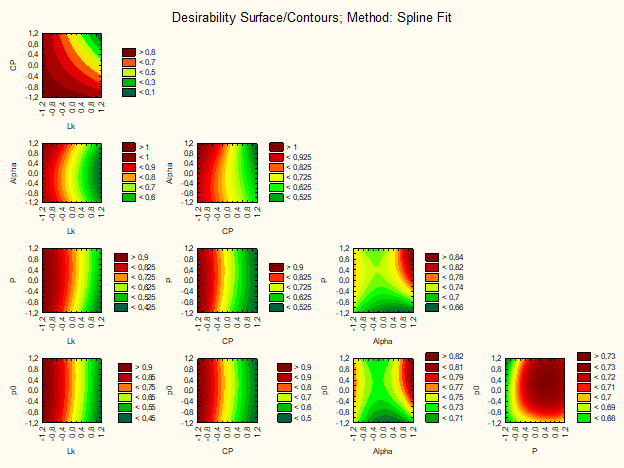
\includegraphics[width=1\textwidth]{P2M1_NNGV_tempo_DSC}
\end{figure}



\begin{table}[H]
\caption{Effect Estimates; Var.:Trabalhos; R-sqr=,9682; Adj:,947; 4 3-level factors, 1 Blocks, 81 Runs; MS Residual=,1508179; DV: Trabalhos. Modelo 2, problema do número de trabalhos}
\label{tab:P2M1_GV_trabalhos}
\hspace*{-1.2cm} % shift left (tune the value)
\resizebox{1.2\textwidth}{!}{% scale relative to textwidt
\begin{tabular}{lllllllllll}
Factors               & Effect                          & Std.Err                         & t(48)                          & p                               & -95,\%Cnf.Limt                  & +95,\%Cnf.Limt                  & Coeff.                          & Std.Err.Coeff.                  & -95,\%Cnf.Limt                  & +95,\%Cnf.Limt                  \\
\rowcolor[HTML]{FFFFFF} 
Mean/Interc.   & {\color[HTML]{FF0000} -32,3951} & {\color[HTML]{FF0000} 0,043150} & {\color[HTML]{FF0000} -750,749} & {\color[HTML]{FF0000} 0,000000} & {\color[HTML]{FF0000} -32,4818} & {\color[HTML]{FF0000} -32,3083} & {\color[HTML]{FF0000} -32,3951} & {\color[HTML]{FF0000} 0,043150} & {\color[HTML]{FF0000} -32,4818} & {\color[HTML]{FF0000} -32,3083} \\
\rowcolor[HTML]{FFFFFF} 
(1)Lk      (L) & {\color[HTML]{FF0000} -1,3667}  & {\color[HTML]{FF0000} 0,105696} & {\color[HTML]{FF0000} -12,930}  & {\color[HTML]{FF0000} 0,000000} & {\color[HTML]{FF0000} -1,5792}  & {\color[HTML]{FF0000} -1,1542}  & {\color[HTML]{FF0000} -0,6833}  & {\color[HTML]{FF0000} 0,052848} & {\color[HTML]{FF0000} -0,7896}  & {\color[HTML]{FF0000} -0,5771}  \\
\rowcolor[HTML]{FFFFFF} 
Lk      (Q)    & {\color[HTML]{FF0000} -0,3019}  & {\color[HTML]{FF0000} 0,091536} & {\color[HTML]{FF0000} -3,298}   & {\color[HTML]{FF0000} 0,001841} & {\color[HTML]{FF0000} -0,4859}  & {\color[HTML]{FF0000} -0,1178}  & {\color[HTML]{FF0000} -0,1509}  & {\color[HTML]{FF0000} 0,045768} & {\color[HTML]{FF0000} -0,2429}  & {\color[HTML]{FF0000} -0,0589}  \\
\rowcolor[HTML]{FFFFFF} 
(2)CP      (L) & {\color[HTML]{FF0000} -2,6074}  & {\color[HTML]{FF0000} 0,105696} & {\color[HTML]{FF0000} -24,669}  & {\color[HTML]{FF0000} 0,000000} & {\color[HTML]{FF0000} -2,8199}  & {\color[HTML]{FF0000} -2,3949}  & {\color[HTML]{FF0000} -1,3037}  & {\color[HTML]{FF0000} 0,052848} & {\color[HTML]{FF0000} -1,4100}  & {\color[HTML]{FF0000} -1,1974}  \\
\rowcolor[HTML]{FFFFFF} 
CP      (Q)    & {\color[HTML]{FF0000} -1,0630}  & {\color[HTML]{FF0000} 0,091536} & {\color[HTML]{FF0000} -11,613}  & {\color[HTML]{FF0000} 0,000000} & {\color[HTML]{FF0000} -1,2470}  & {\color[HTML]{FF0000} -0,8789}  & {\color[HTML]{FF0000} -0,5315}  & {\color[HTML]{FF0000} 0,045768} & {\color[HTML]{FF0000} -0,6235}  & {\color[HTML]{FF0000} -0,4395}  \\
\rowcolor[HTML]{FFFFFF} 
(3)Alpha   (L) & {\color[HTML]{FF0000} 1,1296}   & {\color[HTML]{FF0000} 0,105696} & {\color[HTML]{FF0000} 10,688}   & {\color[HTML]{FF0000} 0,000000} & {\color[HTML]{FF0000} 0,9171}   & {\color[HTML]{FF0000} 1,3421}   & {\color[HTML]{FF0000} 0,5648}   & {\color[HTML]{FF0000} 0,052848} & {\color[HTML]{FF0000} 0,4586}   & {\color[HTML]{FF0000} 0,6711}   \\
\rowcolor[HTML]{FFFFFF} 
Alpha   (Q)    & {\color[HTML]{FF0000} -0,5019}  & {\color[HTML]{FF0000} 0,091536} & {\color[HTML]{FF0000} -5,483}   & {\color[HTML]{FF0000} 0,000002} & {\color[HTML]{FF0000} -0,6859}  & {\color[HTML]{FF0000} -0,3178}  & {\color[HTML]{FF0000} -0,2509}  & {\color[HTML]{FF0000} 0,045768} & {\color[HTML]{FF0000} -0,3429}  & {\color[HTML]{FF0000} -0,1589}  \\
\rowcolor[HTML]{FFFFFF} 
(4)p0      (L) & {\color[HTML]{FF0000} 0,3481}   & {\color[HTML]{FF0000} 0,105696} & {\color[HTML]{FF0000} 3,294}    & {\color[HTML]{FF0000} 0,001861} & {\color[HTML]{FF0000} 0,1356}   & {\color[HTML]{FF0000} 0,5607}   & {\color[HTML]{FF0000} 0,1741}   & {\color[HTML]{FF0000} 0,052848} & {\color[HTML]{FF0000} 0,0678}   & {\color[HTML]{FF0000} 0,2803}   \\
\rowcolor[HTML]{FFFFFF} 
p0      (Q)    & -0,1407                         & 0,091536                        & -1,538                          & 0,130725                        & -0,3248                         & 0,0433                          & -0,0704                         & 0,045768                        & -0,1624                         & 0,0217                          \\
\rowcolor[HTML]{FFFFFF} 
1L by 2L       & 0,1833                          & 0,129451                        & 1,416                           & 0,163163                        & -0,0769                         & 0,4436                          & 0,0917                          & 0,064725                        & -0,0385                         & 0,2218                          \\
\rowcolor[HTML]{FFFFFF} 
1L by 2Q       & -0,0083                         & 0,112108                        & -0,074                          & 0,941054                        & -0,2337                         & 0,2171                          & -0,0042                         & 0,056054                        & -0,1169                         & 0,1085                          \\
\rowcolor[HTML]{FFFFFF} 
1Q by 2L       & 0,1139                          & 0,112108                        & 1,016                           & 0,314777                        & -0,1115                         & 0,3393                          & 0,0569                          & 0,056054                        & -0,0558                         & 0,1696                          \\
\rowcolor[HTML]{FFFFFF} 
1Q by 2Q       & 0,0181                          & 0,097088                        & 0,186                           & 0,853251                        & -0,1772                         & 0,2133                          & 0,0090                          & 0,048544                        & -0,0886                         & 0,1066                          \\
\rowcolor[HTML]{FFFFFF} 
1L by 3L       & 0,1611                          & 0,129451                        & 1,245                           & 0,219332                        & -0,0992                         & 0,4214                          & 0,0806                          & 0,064725                        & -0,0496                         & 0,2107                          \\
\rowcolor[HTML]{FFFFFF} 
1L by 3Q       & 0,0250                          & 0,112108                        & 0,223                           & 0,824482                        & -0,2004                         & 0,2504                          & 0,0125                          & 0,056054                        & -0,1002                         & 0,1252                          \\
\rowcolor[HTML]{FFFFFF} 
1Q by 3L       & 0,0694                          & 0,112108                        & 0,619                           & 0,538554                        & -0,1560                         & 0,2949                          & 0,0347                          & 0,056054                        & -0,0780                         & 0,1474                          \\
\rowcolor[HTML]{FFFFFF} 
1Q by 3Q       & 0,0347                          & 0,097088                        & 0,358                           & 0,722184                        & -0,1605                         & 0,2299                          & 0,0174                          & 0,048544                        & -0,0802                         & 0,1150                          \\
\rowcolor[HTML]{FFFFFF} 
1L by 4L       & -0,0111                         & 0,129451                        & -0,086                          & 0,931957                        & -0,2714                         & 0,2492                          & -0,0056                         & 0,064725                        & -0,1357                         & 0,1246                          \\
\rowcolor[HTML]{FFFFFF} 
1L by 4Q       & 0,0500                          & 0,112108                        & 0,446                           & 0,657603                        & -0,1754                         & 0,2754                          & 0,0250                          & 0,056054                        & -0,0877                         & 0,1377                          \\
\rowcolor[HTML]{FFFFFF} 
1Q by 4L       & -0,1778                         & 0,112108                        & -1,586                          & 0,119357                        & -0,4032                         & 0,0476                          & -0,0889                         & 0,056054                        & -0,2016                         & 0,0238                          \\
\rowcolor[HTML]{FFFFFF} 
1Q by 4Q       & -0,0611                         & 0,097088                        & -0,629                          & 0,532046                        & -0,2563                         & 0,1341                          & -0,0306                         & 0,048544                        & -0,1282                         & 0,0670                          \\
\rowcolor[HTML]{FFFFFF} 
2L by 3L       & {\color[HTML]{FF0000} -1,8722}  & {\color[HTML]{FF0000} 0,129451} & {\color[HTML]{FF0000} -14,463}  & {\color[HTML]{FF0000} 0,000000} & {\color[HTML]{FF0000} -2,1325}  & {\color[HTML]{FF0000} -1,6119}  & {\color[HTML]{FF0000} -0,9361}  & {\color[HTML]{FF0000} 0,064725} & {\color[HTML]{FF0000} -1,0663}  & {\color[HTML]{FF0000} -0,8060}  \\
\rowcolor[HTML]{FFFFFF} 
2L by 3Q       & {\color[HTML]{FF0000} 0,6472}   & {\color[HTML]{FF0000} 0,112108} & {\color[HTML]{FF0000} 5,773}    & {\color[HTML]{FF0000} 0,000001} & {\color[HTML]{FF0000} 0,4218}   & {\color[HTML]{FF0000} 0,8726}   & {\color[HTML]{FF0000} 0,3236}   & {\color[HTML]{FF0000} 0,056054} & {\color[HTML]{FF0000} 0,2109}   & {\color[HTML]{FF0000} 0,4363}   \\
\rowcolor[HTML]{FFFFFF} 
2Q by 3L       & {\color[HTML]{FF0000} -0,9806}  & {\color[HTML]{FF0000} 0,112108} & {\color[HTML]{FF0000} -8,747}   & {\color[HTML]{FF0000} 0,000000} & {\color[HTML]{FF0000} -1,2060}  & {\color[HTML]{FF0000} -0,7551}  & {\color[HTML]{FF0000} -0,4903}  & {\color[HTML]{FF0000} 0,056054} & {\color[HTML]{FF0000} -0,6030}  & {\color[HTML]{FF0000} -0,3776}  \\
\rowcolor[HTML]{FFFFFF} 
2Q by 3Q       & {\color[HTML]{FF0000} 0,3181}   & {\color[HTML]{FF0000} 0,097088} & {\color[HTML]{FF0000} 3,276}    & {\color[HTML]{FF0000} 0,001960} & {\color[HTML]{FF0000} 0,1228}   & {\color[HTML]{FF0000} 0,5133}   & {\color[HTML]{FF0000} 0,1590}   & {\color[HTML]{FF0000} 0,048544} & {\color[HTML]{FF0000} 0,0614}   & {\color[HTML]{FF0000} 0,2566}   \\
\rowcolor[HTML]{FFFFFF} 
2L by 4L       & {\color[HTML]{FF0000} -0,6222}  & {\color[HTML]{FF0000} 0,129451} & {\color[HTML]{FF0000} -4,807}   & {\color[HTML]{FF0000} 0,000016} & {\color[HTML]{FF0000} -0,8825}  & {\color[HTML]{FF0000} -0,3619}  & {\color[HTML]{FF0000} -0,3111}  & {\color[HTML]{FF0000} 0,064725} & {\color[HTML]{FF0000} -0,4413}  & {\color[HTML]{FF0000} -0,1810}  \\
\rowcolor[HTML]{FFFFFF} 
2L by 4Q       & 0,0556                          & 0,112108                        & 0,496                           & 0,622470                        & -0,1699                         & 0,2810                          & 0,0278                          & 0,056054                        & -0,0849                         & 0,1405                          \\
\rowcolor[HTML]{FFFFFF} 
2Q by 4L       & {\color[HTML]{FF0000} -0,2778}  & {\color[HTML]{FF0000} 0,112108} & {\color[HTML]{FF0000} -2,478}   & {\color[HTML]{FF0000} 0,016791} & {\color[HTML]{FF0000} -0,5032}  & {\color[HTML]{FF0000} -0,0524}  & {\color[HTML]{FF0000} -0,1389}  & {\color[HTML]{FF0000} 0,056054} & {\color[HTML]{FF0000} -0,2516}  & {\color[HTML]{FF0000} -0,0262}  \\
\rowcolor[HTML]{FFFFFF} 
2Q by 4Q       & 0,0222                          & 0,097088                        & 0,229                           & 0,819929                        & -0,1730                         & 0,2174                          & 0,0111                          & 0,048544                        & -0,0865                         & 0,1087                          \\
\rowcolor[HTML]{FFFFFF} 
3L by 4L       & {\color[HTML]{FF0000} 0,4500}   & {\color[HTML]{FF0000} 0,129451} & {\color[HTML]{FF0000} 3,476}    & {\color[HTML]{FF0000} 0,001090} & {\color[HTML]{FF0000} 0,1897}   & {\color[HTML]{FF0000} 0,7103}   & {\color[HTML]{FF0000} 0,2250}   & {\color[HTML]{FF0000} 0,064725} & {\color[HTML]{FF0000} 0,0949}   & {\color[HTML]{FF0000} 0,3551}   \\
\rowcolor[HTML]{FFFFFF} 
3L by 4Q       & 0,0528                          & 0,112108                        & 0,471                           & 0,639932                        & -0,1726                         & 0,2782                          & 0,0264                          & 0,056054                        & -0,0863                         & 0,1391                          \\
\rowcolor[HTML]{FFFFFF} 
3Q by 4L       & -0,1361                         & 0,112108                        & -1,214                          & 0,230646                        & -0,3615                         & 0,0893                          & -0,0681                         & 0,056054                        & -0,1808                         & 0,0446                          \\
\rowcolor[HTML]{FFFFFF} 
3Q by 4Q       & -0,0986                         & 0,097088                        & -1,016                          & 0,314871                        & -0,2938                         & 0,0966                          & -0,0493                         & 0,048544                        & -0,1469                         & 0,0483                         
\end{tabular}
}
\end{table}

\begin{figure}[H]
\caption{Gráfico de contorno das quatro variáveis relevantes ($L_{k}$, $CP$, $\alpha$, $p_{0}$), relativamente ao número de trabalhos, do Modelo 2 do problema do número de trabalhos}
\centering
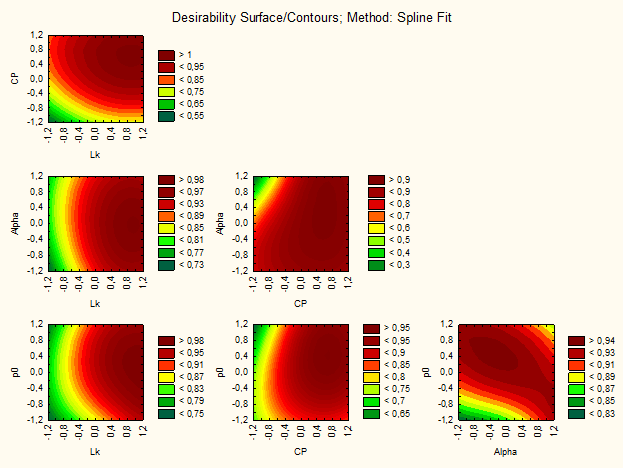
\includegraphics[width=1\textwidth]{P2M1_GV_trabalhos_DSC}
\end{figure}

\begin{table}[H]
\caption{Effect Estimates; Var.:Tempo; R-sqr=,96531; Adj:,94218; 4 3-level factors, 1 Blocks, 81 Runs; MS Residual=4,781419; DV: Tempo. Modelo 2, problema do número de trabalhos}
\label{tab:P2M1_GV_tempo}
\hspace*{-1.2cm} % shift left (tune the value)
\resizebox{1.2\textwidth}{!}{% scale relative to textwidt
\begin{tabular}{lllllllllll}
Factors               & Effect                          & Std.Err                         & t(48)                          & p                               & -95,\%Cnf.Limt                  & +95,\%Cnf.Limt                  & Coeff.                           & Std.Err.Coeff.                  & -95,\%Cnf.Limt                  & +95,\%Cnf.Limt                   \\
\rowcolor[HTML]{FFFFFF} 
Mean/Interc.   & {\color[HTML]{FF0000} 8,65433}  & {\color[HTML]{FF0000} 0,242961} & {\color[HTML]{FF0000} 35,62029} & {\color[HTML]{FF0000} 0,000000} & {\color[HTML]{FF0000} 8,16582}  & {\color[HTML]{FF0000} 9,14283}  & {\color[HTML]{FF0000} 8,654328}  & {\color[HTML]{FF0000} 0,242961} & {\color[HTML]{FF0000} 8,16582}  & {\color[HTML]{FF0000} 9,142833}  \\
\rowcolor[HTML]{FFFFFF} 
(1)Lk      (L) & {\color[HTML]{FF0000} 14,24014} & {\color[HTML]{FF0000} 0,595130} & {\color[HTML]{FF0000} 23,92780} & {\color[HTML]{FF0000} 0,000000} & {\color[HTML]{FF0000} 13,04356} & {\color[HTML]{FF0000} 15,43673} & {\color[HTML]{FF0000} 7,120072}  & {\color[HTML]{FF0000} 0,297565} & {\color[HTML]{FF0000} 6,52178}  & {\color[HTML]{FF0000} 7,718366}  \\
\rowcolor[HTML]{FFFFFF} 
Lk      (Q)    & {\color[HTML]{333333} -0,97820} & {\color[HTML]{333333} 0,515397} & {\color[HTML]{333333} -1,89794} & {\color[HTML]{333333} 0,063726} & {\color[HTML]{333333} -2,01447} & {\color[HTML]{333333} 0,05808}  & {\color[HTML]{333333} -0,489098} & {\color[HTML]{333333} 0,257699} & {\color[HTML]{333333} -1,00724} & {\color[HTML]{333333} 0,029040}  \\
\rowcolor[HTML]{FFFFFF} 
(2)CP      (L) & {\color[HTML]{FF0000} 11,24531} & {\color[HTML]{FF0000} 0,595130} & {\color[HTML]{FF0000} 18,89557} & {\color[HTML]{FF0000} 0,000000} & {\color[HTML]{FF0000} 10,04873} & {\color[HTML]{FF0000} 12,44190} & {\color[HTML]{FF0000} 5,622657}  & {\color[HTML]{FF0000} 0,297565} & {\color[HTML]{FF0000} 5,02436}  & {\color[HTML]{FF0000} 6,220951}  \\
\rowcolor[HTML]{FFFFFF} 
CP      (Q)    & {\color[HTML]{FF0000} 1,38678}  & {\color[HTML]{FF0000} 0,515397} & {\color[HTML]{FF0000} 2,69071}  & {\color[HTML]{FF0000} 0,009782} & {\color[HTML]{FF0000} 0,35051}  & {\color[HTML]{FF0000} 2,42306}  & {\color[HTML]{FF0000} 0,693392}  & {\color[HTML]{FF0000} 0,257699} & {\color[HTML]{FF0000} 0,17525}  & {\color[HTML]{FF0000} 1,211530}  \\
\rowcolor[HTML]{FFFFFF} 
(3)Alpha   (L) & {\color[HTML]{FF0000} 4,87821}  & {\color[HTML]{FF0000} 0,595130} & {\color[HTML]{FF0000} 8,19689}  & {\color[HTML]{FF0000} 0,000000} & {\color[HTML]{FF0000} 3,68162}  & {\color[HTML]{FF0000} 6,07480}  & {\color[HTML]{FF0000} 2,439105}  & {\color[HTML]{FF0000} 0,297565} & {\color[HTML]{FF0000} 1,84081}  & {\color[HTML]{FF0000} 3,037399}  \\
\rowcolor[HTML]{FFFFFF} 
Alpha   (Q)    & {\color[HTML]{FF0000} -1,40244} & {\color[HTML]{FF0000} 0,515397} & {\color[HTML]{FF0000} -2,72109} & {\color[HTML]{FF0000} 0,009037} & {\color[HTML]{FF0000} -2,43872} & {\color[HTML]{FF0000} -0,36616} & {\color[HTML]{FF0000} -0,701220} & {\color[HTML]{FF0000} 0,257699} & {\color[HTML]{FF0000} -1,21936} & {\color[HTML]{FF0000} -0,183082} \\
\rowcolor[HTML]{FFFFFF} 
(4)p0      (L) & {\color[HTML]{FF0000} 3,31278}  & {\color[HTML]{FF0000} 0,595130} & {\color[HTML]{FF0000} 5,56648}  & {\color[HTML]{FF0000} 0,000001} & {\color[HTML]{FF0000} 2,11619}  & {\color[HTML]{FF0000} 4,50936}  & {\color[HTML]{FF0000} 1,656388}  & {\color[HTML]{FF0000} 0,297565} & {\color[HTML]{FF0000} 1,05809}  & {\color[HTML]{FF0000} 2,254682}  \\
\rowcolor[HTML]{FFFFFF} 
p0      (Q)    & {\color[HTML]{333333} -0,65114} & {\color[HTML]{333333} 0,515397} & {\color[HTML]{333333} -1,26338} & {\color[HTML]{333333} 0,212554} & {\color[HTML]{333333} -1,68742} & {\color[HTML]{333333} 0,38513}  & {\color[HTML]{333333} -0,325572} & {\color[HTML]{333333} 0,257699} & {\color[HTML]{333333} -0,84371} & {\color[HTML]{333333} 0,192566}  \\
\rowcolor[HTML]{FFFFFF} 
1L by 2L       & {\color[HTML]{FF0000} 9,44954}  & {\color[HTML]{FF0000} 0,728882} & {\color[HTML]{FF0000} 12,96443} & {\color[HTML]{FF0000} 0,000000} & {\color[HTML]{FF0000} 7,98402}  & {\color[HTML]{FF0000} 10,91505} & {\color[HTML]{FF0000} 4,724768}  & {\color[HTML]{FF0000} 0,364441} & {\color[HTML]{FF0000} 3,99201}  & {\color[HTML]{FF0000} 5,457525}  \\
\rowcolor[HTML]{FFFFFF} 
1L by 2Q       & {\color[HTML]{333333} 1,23266}  & {\color[HTML]{333333} 0,631230} & {\color[HTML]{333333} 1,95280}  & {\color[HTML]{333333} 0,056688} & {\color[HTML]{333333} -0,03651} & {\color[HTML]{333333} 2,50184}  & {\color[HTML]{333333} 0,616332}  & {\color[HTML]{333333} 0,315615} & {\color[HTML]{333333} -0,01825} & {\color[HTML]{333333} 1,250918}  \\
\rowcolor[HTML]{FFFFFF} 
1Q by 2L       & {\color[HTML]{333333} -0,64606} & {\color[HTML]{333333} 0,631230} & {\color[HTML]{333333} -1,02349} & {\color[HTML]{333333} 0,311207} & {\color[HTML]{333333} -1,91523} & {\color[HTML]{333333} 0,62312}  & {\color[HTML]{333333} -0,323029} & {\color[HTML]{333333} 0,315615} & {\color[HTML]{333333} -0,95762} & {\color[HTML]{333333} 0,311558}  \\
\rowcolor[HTML]{FFFFFF} 
1Q by 2Q       & {\color[HTML]{333333} -0,15408} & {\color[HTML]{333333} 0,546661} & {\color[HTML]{333333} -0,28185} & {\color[HTML]{333333} 0,779268} & {\color[HTML]{333333} -1,25321} & {\color[HTML]{333333} 0,94506}  & {\color[HTML]{333333} -0,077039} & {\color[HTML]{333333} 0,273331} & {\color[HTML]{333333} -0,62661} & {\color[HTML]{333333} 0,472529}  \\
\rowcolor[HTML]{FFFFFF} 
1L by 3L       & {\color[HTML]{FF0000} 4,33044}  & {\color[HTML]{FF0000} 0,728882} & {\color[HTML]{FF0000} 5,94121}  & {\color[HTML]{FF0000} 0,000000} & {\color[HTML]{FF0000} 2,86492}  & {\color[HTML]{FF0000} 5,79596}  & {\color[HTML]{FF0000} 2,165220}  & {\color[HTML]{FF0000} 0,364441} & {\color[HTML]{FF0000} 1,43246}  & {\color[HTML]{FF0000} 2,897978}  \\
\rowcolor[HTML]{FFFFFF} 
1L by 3Q       & {\color[HTML]{333333} -1,26857} & {\color[HTML]{333333} 0,631230} & {\color[HTML]{333333} -2,00967} & {\color[HTML]{333333} 0,050105} & {\color[HTML]{333333} -2,53774} & {\color[HTML]{333333} 0,00061}  & {\color[HTML]{333333} -0,634283} & {\color[HTML]{333333} 0,315615} & {\color[HTML]{333333} -1,26887} & {\color[HTML]{333333} 0,000303}  \\
\rowcolor[HTML]{FFFFFF} 
1Q by 3L       & {\color[HTML]{333333} -0,26415} & {\color[HTML]{333333} 0,631230} & {\color[HTML]{333333} -0,41847} & {\color[HTML]{333333} 0,677472} & {\color[HTML]{333333} -1,53332} & {\color[HTML]{333333} 1,00502}  & {\color[HTML]{333333} -0,132075} & {\color[HTML]{333333} 0,315615} & {\color[HTML]{333333} -0,76666} & {\color[HTML]{333333} 0,502512}  \\
\rowcolor[HTML]{FFFFFF} 
1Q by 3Q       & {\color[HTML]{333333} 0,20539}  & {\color[HTML]{333333} 0,546661} & {\color[HTML]{333333} 0,37571}  & {\color[HTML]{333333} 0,708787} & {\color[HTML]{333333} -0,89375} & {\color[HTML]{333333} 1,30452}  & {\color[HTML]{333333} 0,102693}  & {\color[HTML]{333333} 0,273331} & {\color[HTML]{333333} -0,44687} & {\color[HTML]{333333} 0,652262}  \\
\rowcolor[HTML]{FFFFFF} 
1L by 4L       & {\color[HTML]{FF0000} 2,56135}  & {\color[HTML]{FF0000} 0,728882} & {\color[HTML]{FF0000} 3,51408}  & {\color[HTML]{FF0000} 0,000973} & {\color[HTML]{FF0000} 1,09583}  & {\color[HTML]{FF0000} 4,02686}  & {\color[HTML]{FF0000} 1,280673}  & {\color[HTML]{FF0000} 0,364441} & {\color[HTML]{FF0000} 0,54792}  & {\color[HTML]{FF0000} 2,013431}  \\
\rowcolor[HTML]{FFFFFF} 
1L by 4Q       & {\color[HTML]{333333} -0,61920} & {\color[HTML]{333333} 0,631230} & {\color[HTML]{333333} -0,98095} & {\color[HTML]{333333} 0,331538} & {\color[HTML]{333333} -1,88838} & {\color[HTML]{333333} 0,64997}  & {\color[HTML]{333333} -0,309601} & {\color[HTML]{333333} 0,315615} & {\color[HTML]{333333} -0,94419} & {\color[HTML]{333333} 0,324986}  \\
\rowcolor[HTML]{FFFFFF} 
1Q by 4L       & {\color[HTML]{333333} 0,08346}  & {\color[HTML]{333333} 0,631230} & {\color[HTML]{333333} 0,13222}  & {\color[HTML]{333333} 0,895360} & {\color[HTML]{333333} -1,18571} & {\color[HTML]{333333} 1,35264}  & {\color[HTML]{333333} 0,041732}  & {\color[HTML]{333333} 0,315615} & {\color[HTML]{333333} -0,59285} & {\color[HTML]{333333} 0,676319}  \\
\rowcolor[HTML]{FFFFFF} 
1Q by 4Q       & {\color[HTML]{333333} 0,14914}  & {\color[HTML]{333333} 0,546661} & {\color[HTML]{333333} 0,27282}  & {\color[HTML]{333333} 0,786159} & {\color[HTML]{333333} -0,94999} & {\color[HTML]{333333} 1,24828}  & {\color[HTML]{333333} 0,074571}  & {\color[HTML]{333333} 0,273331} & {\color[HTML]{333333} -0,47500} & {\color[HTML]{333333} 0,624139}  \\
\rowcolor[HTML]{FFFFFF} 
2L by 3L       & {\color[HTML]{FF0000} 3,42415}  & {\color[HTML]{FF0000} 0,728882} & {\color[HTML]{FF0000} 4,69781}  & {\color[HTML]{FF0000} 0,000022} & {\color[HTML]{FF0000} 1,95864}  & {\color[HTML]{FF0000} 4,88967}  & {\color[HTML]{FF0000} 1,712076}  & {\color[HTML]{FF0000} 0,364441} & {\color[HTML]{FF0000} 0,97932}  & {\color[HTML]{FF0000} 2,444834}  \\
\rowcolor[HTML]{FFFFFF} 
2L by 3Q       & {\color[HTML]{FF0000} -1,45811} & {\color[HTML]{FF0000} 0,631230} & {\color[HTML]{FF0000} -2,30995} & {\color[HTML]{FF0000} 0,025236} & {\color[HTML]{FF0000} -2,72728} & {\color[HTML]{FF0000} -0,18894} & {\color[HTML]{FF0000} -0,729055} & {\color[HTML]{FF0000} 0,315615} & {\color[HTML]{FF0000} -1,36364} & {\color[HTML]{FF0000} -0,094468} \\
\rowcolor[HTML]{FFFFFF} 
2Q by 3L       & {\color[HTML]{FF0000} 1,85433}  & {\color[HTML]{FF0000} 0,631230} & {\color[HTML]{FF0000} 2,93765}  & {\color[HTML]{FF0000} 0,005068} & {\color[HTML]{FF0000} 0,58516}  & {\color[HTML]{FF0000} 3,12351}  & {\color[HTML]{FF0000} 0,927167}  & {\color[HTML]{FF0000} 0,315615} & {\color[HTML]{FF0000} 0,29258}  & {\color[HTML]{FF0000} 1,561754}  \\
\rowcolor[HTML]{FFFFFF} 
2Q by 3Q       & {\color[HTML]{333333} -0,68210} & {\color[HTML]{333333} 0,546661} & {\color[HTML]{333333} -1,24776} & {\color[HTML]{333333} 0,218171} & {\color[HTML]{333333} -1,78124} & {\color[HTML]{333333} 0,41703}  & {\color[HTML]{333333} -0,341052} & {\color[HTML]{333333} 0,273331} & {\color[HTML]{333333} -0,89062} & {\color[HTML]{333333} 0,208516}  \\
\rowcolor[HTML]{FFFFFF} 
2L by 4L       & {\color[HTML]{333333} 1,40334}  & {\color[HTML]{333333} 0,728882} & {\color[HTML]{333333} 1,92533}  & {\color[HTML]{333333} 0,060124} & {\color[HTML]{333333} -0,06218} & {\color[HTML]{333333} 2,86885}  & {\color[HTML]{333333} 0,701669}  & {\color[HTML]{333333} 0,364441} & {\color[HTML]{333333} -0,03109} & {\color[HTML]{333333} 1,434427}  \\
\rowcolor[HTML]{FFFFFF} 
2L by 4Q       & {\color[HTML]{333333} -0,33241} & {\color[HTML]{333333} 0,631230} & {\color[HTML]{333333} -0,52661} & {\color[HTML]{333333} 0,600891} & {\color[HTML]{333333} -1,60158} & {\color[HTML]{333333} 0,93676}  & {\color[HTML]{333333} -0,166205} & {\color[HTML]{333333} 0,315615} & {\color[HTML]{333333} -0,80079} & {\color[HTML]{333333} 0,468381}  \\
\rowcolor[HTML]{FFFFFF} 
2Q by 4L       & {\color[HTML]{333333} 0,71261}  & {\color[HTML]{333333} 0,631230} & {\color[HTML]{333333} 1,12892}  & {\color[HTML]{333333} 0,264543} & {\color[HTML]{333333} -0,55657} & {\color[HTML]{333333} 1,98178}  & {\color[HTML]{333333} 0,356304}  & {\color[HTML]{333333} 0,315615} & {\color[HTML]{333333} -0,27828} & {\color[HTML]{333333} 0,990890}  \\
\rowcolor[HTML]{FFFFFF} 
2Q by 4Q       & {\color[HTML]{333333} -0,07090} & {\color[HTML]{333333} 0,546661} & {\color[HTML]{333333} -0,12970} & {\color[HTML]{333333} 0,897348} & {\color[HTML]{333333} -1,17004} & {\color[HTML]{333333} 1,02824}  & {\color[HTML]{333333} -0,035450} & {\color[HTML]{333333} 0,273331} & {\color[HTML]{333333} -0,58502} & {\color[HTML]{333333} 0,514118}  \\
\rowcolor[HTML]{FFFFFF} 
3L by 4L       & {\color[HTML]{FF0000} 2,89770}  & {\color[HTML]{FF0000} 0,728882} & {\color[HTML]{FF0000} 3,97555}  & {\color[HTML]{FF0000} 0,000236} & {\color[HTML]{FF0000} 1,43219}  & {\color[HTML]{FF0000} 4,36322}  & {\color[HTML]{FF0000} 1,448852}  & {\color[HTML]{FF0000} 0,364441} & {\color[HTML]{FF0000} 0,71609}  & {\color[HTML]{FF0000} 2,181610}  \\
\rowcolor[HTML]{FFFFFF} 
3L by 4Q       & {\color[HTML]{333333} -0,66724} & {\color[HTML]{333333} 0,631230} & {\color[HTML]{333333} -1,05704} & {\color[HTML]{333333} 0,295783} & {\color[HTML]{333333} -1,93641} & {\color[HTML]{333333} 0,60194}  & {\color[HTML]{333333} -0,333618} & {\color[HTML]{333333} 0,315615} & {\color[HTML]{333333} -0,96821} & {\color[HTML]{333333} 0,300968}  \\
\rowcolor[HTML]{FFFFFF} 
3Q by 4L       & {\color[HTML]{333333} -0,88979} & {\color[HTML]{333333} 0,631230} & {\color[HTML]{333333} -1,40961} & {\color[HTML]{333333} 0,165101} & {\color[HTML]{333333} -2,15896} & {\color[HTML]{333333} 0,37938}  & {\color[HTML]{333333} -0,444895} & {\color[HTML]{333333} 0,315615} & {\color[HTML]{333333} -1,07948} & {\color[HTML]{333333} 0,189692}  \\
\rowcolor[HTML]{FFFFFF} 
3Q by 4Q       & {\color[HTML]{333333} 0,12124}  & {\color[HTML]{333333} 0,546661} & {\color[HTML]{333333} 0,22178}  & {\color[HTML]{333333} 0,825423} & {\color[HTML]{333333} -0,97790} & {\color[HTML]{333333} 1,22038}  & {\color[HTML]{333333} 0,060620}  & {\color[HTML]{333333} 0,273331} & {\color[HTML]{333333} -0,48895} & {\color[HTML]{333333} 0,610189} 
\end{tabular}
}
\end{table}

\begin{figure}[H]
\caption{Gráfico de contorno das quatro variáveis relevantes ($L_{k}$, $CP$, $\alpha$, $p_{0}$), relativamente ao tempo, do Modelo 2 do problema do número de trabalhos}
\centering
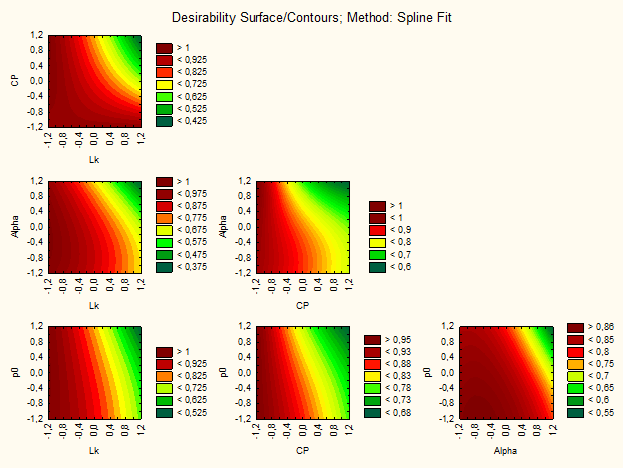
\includegraphics[width=1\textwidth]{P2M1_GV_tempo_DSC}
\end{figure}



\begin{table}[H]
\caption{Effect Estimates; Var.:Trabalhos; R-sqr=,94694; Adj:,91156; 4 3-level factors, 1 Blocks, 81 Runs; MS Residual=,0347377; DV: Trabalhos. Modelo 3, problema do número de trabalhos}
\label{tab:P2M2_GV_trabalhos}
\hspace*{-1.2cm} % shift left (tune the value)
\resizebox{1.2\textwidth}{!}{% scale relative to textwidt
\begin{tabular}{lllllllllll}
Factors        & Effect                          & Std.Err                         & t(48)                          & p                               & -95,\%Cnf.Limt                  & +95,\%Cnf.Limt                  & Coeff.                          & Std.Err.Coeff.                  & -95,\%Cnf.Limt                  & +95,\%Cnf.Limt                  \\
\rowcolor[HTML]{FFFFFF} 
Mean/Interc.   & {\color[HTML]{FF0000} -33,4346} & {\color[HTML]{FF0000} 0,020709} & {\color[HTML]{FF0000} -1614,50} & {\color[HTML]{FF0000} 0,000000} & {\color[HTML]{FF0000} -33,4762} & {\color[HTML]{FF0000} -33,3929} & {\color[HTML]{FF0000} -33,4346} & {\color[HTML]{FF0000} 0,020709} & {\color[HTML]{FF0000} -33,4762} & {\color[HTML]{FF0000} -33,3929} \\
\rowcolor[HTML]{FFFFFF} 
(1)Lk      (L) & {\color[HTML]{FF0000} -0,2481}  & {\color[HTML]{FF0000} 0,050726} & {\color[HTML]{FF0000} -4,89}    & {\color[HTML]{FF0000} 0,000012} & {\color[HTML]{FF0000} -0,3501}  & {\color[HTML]{FF0000} -0,1462}  & {\color[HTML]{FF0000} -0,1241}  & {\color[HTML]{FF0000} 0,025363} & {\color[HTML]{FF0000} -0,1751}  & {\color[HTML]{FF0000} -0,0731}  \\
\rowcolor[HTML]{FFFFFF} 
Lk      (Q)    & {\color[HTML]{333333} -0,0204}  & {\color[HTML]{333333} 0,043930} & {\color[HTML]{333333} -0,46}    & {\color[HTML]{333333} 0,644960} & {\color[HTML]{333333} -0,1087}  & {\color[HTML]{333333} 0,0680}   & {\color[HTML]{333333} -0,0102}  & {\color[HTML]{333333} 0,021965} & {\color[HTML]{333333} -0,0543}  & {\color[HTML]{333333} 0,0340}   \\
\rowcolor[HTML]{FFFFFF} 
(2)CP      (L) & {\color[HTML]{FF0000} -1,1519}  & {\color[HTML]{FF0000} 0,050726} & {\color[HTML]{FF0000} -22,71}   & {\color[HTML]{FF0000} 0,000000} & {\color[HTML]{FF0000} -1,2538}  & {\color[HTML]{FF0000} -1,0499}  & {\color[HTML]{FF0000} -0,5759}  & {\color[HTML]{FF0000} 0,025363} & {\color[HTML]{FF0000} -0,6269}  & {\color[HTML]{FF0000} -0,5249}  \\
\rowcolor[HTML]{FFFFFF} 
CP      (Q)    & {\color[HTML]{FF0000} -0,3537}  & {\color[HTML]{FF0000} 0,043930} & {\color[HTML]{FF0000} -8,05}    & {\color[HTML]{FF0000} 0,000000} & {\color[HTML]{FF0000} -0,4420}  & {\color[HTML]{FF0000} -0,2654}  & {\color[HTML]{FF0000} -0,1769}  & {\color[HTML]{FF0000} 0,021965} & {\color[HTML]{FF0000} -0,2210}  & {\color[HTML]{FF0000} -0,1327}  \\
\rowcolor[HTML]{FFFFFF} 
(3)Alpha   (L) & {\color[HTML]{FF0000} 0,5074}   & {\color[HTML]{FF0000} 0,050726} & {\color[HTML]{FF0000} 10,00}    & {\color[HTML]{FF0000} 0,000000} & {\color[HTML]{FF0000} 0,4054}   & {\color[HTML]{FF0000} 0,6094}   & {\color[HTML]{FF0000} 0,2537}   & {\color[HTML]{FF0000} 0,025363} & {\color[HTML]{FF0000} 0,2027}   & {\color[HTML]{FF0000} 0,3047}   \\
\rowcolor[HTML]{FFFFFF} 
Alpha   (Q)    & {\color[HTML]{FF0000} -0,1537}  & {\color[HTML]{FF0000} 0,043930} & {\color[HTML]{FF0000} -3,50}    & {\color[HTML]{FF0000} 0,001019} & {\color[HTML]{FF0000} -0,2420}  & {\color[HTML]{FF0000} -0,0654}  & {\color[HTML]{FF0000} -0,0769}  & {\color[HTML]{FF0000} 0,021965} & {\color[HTML]{FF0000} -0,1210}  & {\color[HTML]{FF0000} -0,0327}  \\
\rowcolor[HTML]{FFFFFF} 
(4)p0      (L) & {\color[HTML]{FF0000} 0,4259}   & {\color[HTML]{FF0000} 0,050726} & {\color[HTML]{FF0000} 8,40}     & {\color[HTML]{FF0000} 0,000000} & {\color[HTML]{FF0000} 0,3239}   & {\color[HTML]{FF0000} 0,5279}   & {\color[HTML]{FF0000} 0,2130}   & {\color[HTML]{FF0000} 0,025363} & {\color[HTML]{FF0000} 0,1620}   & {\color[HTML]{FF0000} 0,2640}   \\
\rowcolor[HTML]{FFFFFF} 
p0      (Q)    & {\color[HTML]{333333} -0,0537}  & {\color[HTML]{333333} 0,043930} & {\color[HTML]{333333} -1,22}    & {\color[HTML]{333333} 0,227497} & {\color[HTML]{333333} -0,1420}  & {\color[HTML]{333333} 0,0346}   & {\color[HTML]{333333} -0,0269}  & {\color[HTML]{333333} 0,021965} & {\color[HTML]{333333} -0,0710}  & {\color[HTML]{333333} 0,0173}   \\
\rowcolor[HTML]{FFFFFF} 
1L by 2L       & {\color[HTML]{FF0000} 0,1611}   & {\color[HTML]{FF0000} 0,062127} & {\color[HTML]{FF0000} 2,59}     & {\color[HTML]{FF0000} 0,012566} & {\color[HTML]{FF0000} 0,0362}   & {\color[HTML]{FF0000} 0,2860}   & {\color[HTML]{FF0000} 0,0806}   & {\color[HTML]{FF0000} 0,031063} & {\color[HTML]{FF0000} 0,0181}   & {\color[HTML]{FF0000} 0,1430}   \\
\rowcolor[HTML]{FFFFFF} 
1L by 2Q       & {\color[HTML]{333333} 0,0194}   & {\color[HTML]{333333} 0,053803} & {\color[HTML]{333333} 0,36}     & {\color[HTML]{333333} 0,719388} & {\color[HTML]{333333} -0,0887}  & {\color[HTML]{333333} 0,1276}   & {\color[HTML]{333333} 0,0097}   & {\color[HTML]{333333} 0,026902} & {\color[HTML]{333333} -0,0444}  & {\color[HTML]{333333} 0,0638}   \\
\rowcolor[HTML]{FFFFFF} 
1Q by 2L       & {\color[HTML]{333333} 0,0139}   & {\color[HTML]{333333} 0,053803} & {\color[HTML]{333333} 0,26}     & {\color[HTML]{333333} 0,797401} & {\color[HTML]{333333} -0,0943}  & {\color[HTML]{333333} 0,1221}   & {\color[HTML]{333333} 0,0069}   & {\color[HTML]{333333} 0,026902} & {\color[HTML]{333333} -0,0471}  & {\color[HTML]{333333} 0,0610}   \\
\rowcolor[HTML]{FFFFFF} 
1Q by 2Q       & {\color[HTML]{333333} -0,0181}  & {\color[HTML]{333333} 0,046595} & {\color[HTML]{333333} -0,39}    & {\color[HTML]{333333} 0,700100} & {\color[HTML]{333333} -0,1117}  & {\color[HTML]{333333} 0,0756}   & {\color[HTML]{333333} -0,0090}  & {\color[HTML]{333333} 0,023298} & {\color[HTML]{333333} -0,0559}  & {\color[HTML]{333333} 0,0378}   \\
\rowcolor[HTML]{FFFFFF} 
1L by 3L       & {\color[HTML]{333333} 0,0444}   & {\color[HTML]{333333} 0,062127} & {\color[HTML]{333333} 0,72}     & {\color[HTML]{333333} 0,477838} & {\color[HTML]{333333} -0,0805}  & {\color[HTML]{333333} 0,1694}   & {\color[HTML]{333333} 0,0222}   & {\color[HTML]{333333} 0,031063} & {\color[HTML]{333333} -0,0402}  & {\color[HTML]{333333} 0,0847}   \\
\rowcolor[HTML]{FFFFFF} 
1L by 3Q       & {\color[HTML]{333333} 0,0444}   & {\color[HTML]{333333} 0,053803} & {\color[HTML]{333333} 0,83}     & {\color[HTML]{333333} 0,412861} & {\color[HTML]{333333} -0,0637}  & {\color[HTML]{333333} 0,1526}   & {\color[HTML]{333333} 0,0222}   & {\color[HTML]{333333} 0,026902} & {\color[HTML]{333333} -0,0319}  & {\color[HTML]{333333} 0,0763}   \\
\rowcolor[HTML]{FFFFFF} 
1Q by 3L       & {\color[HTML]{333333} 0,0278}   & {\color[HTML]{333333} 0,053803} & {\color[HTML]{333333} 0,52}     & {\color[HTML]{333333} 0,608027} & {\color[HTML]{333333} -0,0804}  & {\color[HTML]{333333} 0,1360}   & {\color[HTML]{333333} 0,0139}   & {\color[HTML]{333333} 0,026902} & {\color[HTML]{333333} -0,0402}  & {\color[HTML]{333333} 0,0680}   \\
\rowcolor[HTML]{FFFFFF} 
1Q by 3Q       & {\color[HTML]{333333} -0,0306}  & {\color[HTML]{333333} 0,046595} & {\color[HTML]{333333} -0,66}    & {\color[HTML]{333333} 0,515105} & {\color[HTML]{333333} -0,1242}  & {\color[HTML]{333333} 0,0631}   & {\color[HTML]{333333} -0,0153}  & {\color[HTML]{333333} 0,023298} & {\color[HTML]{333333} -0,0621}  & {\color[HTML]{333333} 0,0316}   \\
\rowcolor[HTML]{FFFFFF} 
1L by 4L       & {\color[HTML]{333333} -0,0111}  & {\color[HTML]{333333} 0,062127} & {\color[HTML]{333333} -0,18}    & {\color[HTML]{333333} 0,858812} & {\color[HTML]{333333} -0,1360}  & {\color[HTML]{333333} 0,1138}   & {\color[HTML]{333333} -0,0056}  & {\color[HTML]{333333} 0,031063} & {\color[HTML]{333333} -0,0680}  & {\color[HTML]{333333} 0,0569}   \\
\rowcolor[HTML]{FFFFFF} 
1L by 4Q       & {\color[HTML]{333333} 0,0111}   & {\color[HTML]{333333} 0,053803} & {\color[HTML]{333333} 0,21}     & {\color[HTML]{333333} 0,837264} & {\color[HTML]{333333} -0,0971}  & {\color[HTML]{333333} 0,1193}   & {\color[HTML]{333333} 0,0056}   & {\color[HTML]{333333} 0,026902} & {\color[HTML]{333333} -0,0485}  & {\color[HTML]{333333} 0,0596}   \\
\rowcolor[HTML]{FFFFFF} 
1Q by 4L       & {\color[HTML]{333333} 0,0222}   & {\color[HTML]{333333} 0,053803} & {\color[HTML]{333333} 0,41}     & {\color[HTML]{333333} 0,681427} & {\color[HTML]{333333} -0,0860}  & {\color[HTML]{333333} 0,1304}   & {\color[HTML]{333333} 0,0111}   & {\color[HTML]{333333} 0,026902} & {\color[HTML]{333333} -0,0430}  & {\color[HTML]{333333} 0,0652}   \\
\rowcolor[HTML]{FFFFFF} 
1Q by 4Q       & {\color[HTML]{333333} -0,0306}  & {\color[HTML]{333333} 0,046595} & {\color[HTML]{333333} -0,66}    & {\color[HTML]{333333} 0,515105} & {\color[HTML]{333333} -0,1242}  & {\color[HTML]{333333} 0,0631}   & {\color[HTML]{333333} -0,0153}  & {\color[HTML]{333333} 0,023298} & {\color[HTML]{333333} -0,0621}  & {\color[HTML]{333333} 0,0316}   \\
\rowcolor[HTML]{FFFFFF} 
2L by 3L       & {\color[HTML]{333333} -0,0778}  & {\color[HTML]{333333} 0,062127} & {\color[HTML]{333333} -1,25}    & {\color[HTML]{333333} 0,216665} & {\color[HTML]{333333} -0,2027}  & {\color[HTML]{333333} 0,0471}   & {\color[HTML]{333333} -0,0389}  & {\color[HTML]{333333} 0,031063} & {\color[HTML]{333333} -0,1013}  & {\color[HTML]{333333} 0,0236}   \\
\rowcolor[HTML]{FFFFFF} 
2L by 3Q       & {\color[HTML]{333333} -0,0944}  & {\color[HTML]{333333} 0,053803} & {\color[HTML]{333333} -1,76}    & {\color[HTML]{333333} 0,085578} & {\color[HTML]{333333} -0,2026}  & {\color[HTML]{333333} 0,0137}   & {\color[HTML]{333333} -0,0472}  & {\color[HTML]{333333} 0,026902} & {\color[HTML]{333333} -0,1013}  & {\color[HTML]{333333} 0,0069}   \\
\rowcolor[HTML]{FFFFFF} 
2Q by 3L       & {\color[HTML]{FF0000} 0,1778}   & {\color[HTML]{FF0000} 0,053803} & {\color[HTML]{FF0000} 3,30}     & {\color[HTML]{FF0000} 0,001806} & {\color[HTML]{FF0000} 0,0696}   & {\color[HTML]{FF0000} 0,2860}   & {\color[HTML]{FF0000} 0,0889}   & {\color[HTML]{FF0000} 0,026902} & {\color[HTML]{FF0000} 0,0348}   & {\color[HTML]{FF0000} 0,1430}   \\
\rowcolor[HTML]{FFFFFF} 
2Q by 3Q       & {\color[HTML]{FF0000} -0,1556}  & {\color[HTML]{FF0000} 0,046595} & {\color[HTML]{FF0000} -3,34}    & {\color[HTML]{FF0000} 0,001635} & {\color[HTML]{FF0000} -0,2492}  & {\color[HTML]{FF0000} -0,0619}  & {\color[HTML]{FF0000} -0,0778}  & {\color[HTML]{FF0000} 0,023298} & {\color[HTML]{FF0000} -0,1246}  & {\color[HTML]{FF0000} -0,0309}  \\
\rowcolor[HTML]{FFFFFF} 
2L by 4L       & {\color[HTML]{FF0000} -0,2333}  & {\color[HTML]{FF0000} 0,062127} & {\color[HTML]{FF0000} -3,76}    & {\color[HTML]{FF0000} 0,000467} & {\color[HTML]{FF0000} -0,3582}  & {\color[HTML]{FF0000} -0,1084}  & {\color[HTML]{FF0000} -0,1167}  & {\color[HTML]{FF0000} 0,031063} & {\color[HTML]{FF0000} -0,1791}  & {\color[HTML]{FF0000} -0,0542}  \\
\rowcolor[HTML]{FFFFFF} 
2L by 4Q       & {\color[HTML]{333333} 0,0389}   & {\color[HTML]{333333} 0,053803} & {\color[HTML]{333333} 0,72}     & {\color[HTML]{333333} 0,473312} & {\color[HTML]{333333} -0,0693}  & {\color[HTML]{333333} 0,1471}   & {\color[HTML]{333333} 0,0194}   & {\color[HTML]{333333} 0,026902} & {\color[HTML]{333333} -0,0346}  & {\color[HTML]{333333} 0,0735}   \\
\rowcolor[HTML]{FFFFFF} 
2Q by 4L       & {\color[HTML]{333333} -0,0611}  & {\color[HTML]{333333} 0,053803} & {\color[HTML]{333333} -1,14}    & {\color[HTML]{333333} 0,261670} & {\color[HTML]{333333} -0,1693}  & {\color[HTML]{333333} 0,0471}   & {\color[HTML]{333333} -0,0306}  & {\color[HTML]{333333} 0,026902} & {\color[HTML]{333333} -0,0846}  & {\color[HTML]{333333} 0,0235}   \\
\rowcolor[HTML]{FFFFFF} 
2Q by 4Q       & {\color[HTML]{333333} 0,0194}   & {\color[HTML]{333333} 0,046595} & {\color[HTML]{333333} 0,42}     & {\color[HTML]{333333} 0,678315} & {\color[HTML]{333333} -0,0742}  & {\color[HTML]{333333} 0,1131}   & {\color[HTML]{333333} 0,0097}   & {\color[HTML]{333333} 0,023298} & {\color[HTML]{333333} -0,0371}  & {\color[HTML]{333333} 0,0566}   \\
\rowcolor[HTML]{FFFFFF} 
3L by 4L       & {\color[HTML]{FF0000} 0,2278}   & {\color[HTML]{FF0000} 0,062127} & {\color[HTML]{FF0000} 3,67}     & {\color[HTML]{FF0000} 0,000615} & {\color[HTML]{FF0000} 0,1029}   & {\color[HTML]{FF0000} 0,3527}   & {\color[HTML]{FF0000} 0,1139}   & {\color[HTML]{FF0000} 0,031063} & {\color[HTML]{FF0000} 0,0514}   & {\color[HTML]{FF0000} 0,1763}   \\
\rowcolor[HTML]{FFFFFF} 
3L by 4Q       & {\color[HTML]{333333} 0,0028}   & {\color[HTML]{333333} 0,053803} & {\color[HTML]{333333} 0,05}     & {\color[HTML]{333333} 0,959039} & {\color[HTML]{333333} -0,1054}  & {\color[HTML]{333333} 0,1110}   & {\color[HTML]{333333} 0,0014}   & {\color[HTML]{333333} 0,026902} & {\color[HTML]{333333} -0,0527}  & {\color[HTML]{333333} 0,0555}   \\
\rowcolor[HTML]{FFFFFF} 
3Q by 4L       & {\color[HTML]{333333} -0,0694}  & {\color[HTML]{333333} 0,053803} & {\color[HTML]{333333} -1,29}    & {\color[HTML]{333333} 0,202988} & {\color[HTML]{333333} -0,1776}  & {\color[HTML]{333333} 0,0387}   & {\color[HTML]{333333} -0,0347}  & {\color[HTML]{333333} 0,026902} & {\color[HTML]{333333} -0,0888}  & {\color[HTML]{333333} 0,0194}   \\
\rowcolor[HTML]{FFFFFF} 
3Q by 4Q       & {\color[HTML]{333333} -0,0181}  & {\color[HTML]{333333} 0,046595} & {\color[HTML]{333333} -0,39}    & {\color[HTML]{333333} 0,700100} & {\color[HTML]{333333} -0,1117}  & {\color[HTML]{333333} 0,0756}   & {\color[HTML]{333333} -0,0090}  & {\color[HTML]{333333} 0,023298} & {\color[HTML]{333333} -0,0559}  & {\color[HTML]{333333} 0,0378}  
\end{tabular}
}
\end{table}

\begin{figure}[H]
\caption{Gráfico de contorno das cinco variáveis relevantes ($L_{k}$, $CP$, $\alpha$, $p_{0}$), relativamente ao número de trabalhos, do Modelo 3 do problema do número de trabalhos}
\centering
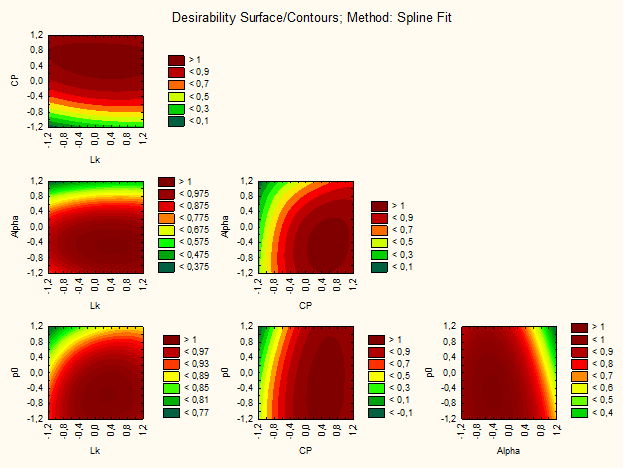
\includegraphics[width=1\textwidth]{P2M2_GV_trabalhos_DSC}
\end{figure}

\begin{table}[H]
\caption{Effect Estimates; Var.:Tempo; R-sqr=,99387; Adj:,98978; 4 3-level factors, 1 Blocks, 81 Runs; MS Residual=2,619281; DV: Tempo. Modelo 3, problema do número de trabalhos}
\label{tab:P2M2_GV_tempo}
\hspace*{-1.2cm} % shift left (tune the value)
\resizebox{1.2\textwidth}{!}{% scale relative to textwi
\begin{tabular}{lllllllllll}
Factors        & Effect                          & Std.Err                         & t(48)                           & p                               & -95,\%Cnf.Limt                  & +95,\%Cnf.Limt                  & Coeff.                          & Std.Err.Coeff.                  & -95,\%Cnf.Limt                  & +95,\%Cnf.Limt                  \\
\rowcolor[HTML]{FFFFFF} 
Mean/Interc.   & {\color[HTML]{FF0000} 17,29346} & {\color[HTML]{FF0000} 0,179824} & {\color[HTML]{FF0000} 96,16862} & {\color[HTML]{FF0000} 0,000000} & {\color[HTML]{FF0000} 16,93190} & {\color[HTML]{FF0000} 17,65502} & {\color[HTML]{FF0000} 17,29346} & {\color[HTML]{FF0000} 0,179824} & {\color[HTML]{FF0000} 16,93190} & {\color[HTML]{FF0000} 17,65502} \\
\rowcolor[HTML]{FFFFFF} 
(1)Lk      (L) & {\color[HTML]{FF0000} 22,35834} & {\color[HTML]{FF0000} 0,440478} & {\color[HTML]{FF0000} 50,75926} & {\color[HTML]{FF0000} 0,000000} & {\color[HTML]{FF0000} 21,47270} & {\color[HTML]{FF0000} 23,24398} & {\color[HTML]{FF0000} 11,17917} & {\color[HTML]{FF0000} 0,220239} & {\color[HTML]{FF0000} 10,73635} & {\color[HTML]{FF0000} 11,62199} \\
\rowcolor[HTML]{FFFFFF} 
Lk      (Q)    & {\color[HTML]{181A1B} 0,01320}  & {\color[HTML]{181A1B} 0,381465} & {\color[HTML]{181A1B} 0,03460}  & {\color[HTML]{181A1B} 0,972539} & {\color[HTML]{181A1B} -0,75379} & {\color[HTML]{181A1B} 0,78019}  & {\color[HTML]{181A1B} 0,00660}  & {\color[HTML]{181A1B} 0,190733} & {\color[HTML]{181A1B} -0,37689} & {\color[HTML]{181A1B} 0,39009}  \\
\rowcolor[HTML]{FFFFFF} 
(2)CP      (L) & {\color[HTML]{FF0000} 27,91703} & {\color[HTML]{FF0000} 0,440478} & {\color[HTML]{FF0000} 63,37895} & {\color[HTML]{FF0000} 0,000000} & {\color[HTML]{FF0000} 27,03139} & {\color[HTML]{FF0000} 28,80267} & {\color[HTML]{FF0000} 13,95852} & {\color[HTML]{FF0000} 0,220239} & {\color[HTML]{FF0000} 13,51570} & {\color[HTML]{FF0000} 14,40134} \\
\rowcolor[HTML]{FFFFFF} 
CP      (Q)    & {\color[HTML]{181A1B} 0,17597}  & {\color[HTML]{181A1B} 0,381465} & {\color[HTML]{181A1B} 0,46130}  & {\color[HTML]{181A1B} 0,646665} & {\color[HTML]{181A1B} -0,59102} & {\color[HTML]{181A1B} 0,94296}  & {\color[HTML]{181A1B} 0,08799}  & {\color[HTML]{181A1B} 0,190733} & {\color[HTML]{181A1B} -0,29551} & {\color[HTML]{181A1B} 0,47148}  \\
\rowcolor[HTML]{FFFFFF} 
(3)Alpha   (L) & {\color[HTML]{FF0000} 1,03598}  & {\color[HTML]{FF0000} 0,440478} & {\color[HTML]{FF0000} 2,35194}  & {\color[HTML]{FF0000} 0,022826} & {\color[HTML]{FF0000} 0,15034}  & {\color[HTML]{FF0000} 1,92162}  & {\color[HTML]{FF0000} 0,51799}  & {\color[HTML]{FF0000} 0,220239} & {\color[HTML]{FF0000} 0,07517}  & {\color[HTML]{FF0000} 0,96081}  \\
\rowcolor[HTML]{FFFFFF} 
Alpha   (Q)    & {\color[HTML]{181A1B} 0,55499}  & {\color[HTML]{181A1B} 0,381465} & {\color[HTML]{181A1B} 1,45490}  & {\color[HTML]{181A1B} 0,152206} & {\color[HTML]{181A1B} -0,21199} & {\color[HTML]{181A1B} 1,32198}  & {\color[HTML]{181A1B} 0,27750}  & {\color[HTML]{181A1B} 0,190733} & {\color[HTML]{181A1B} -0,10600} & {\color[HTML]{181A1B} 0,66099}  \\
\rowcolor[HTML]{FFFFFF} 
(4)p0      (L) & {\color[HTML]{FF0000} 1,58334}  & {\color[HTML]{FF0000} 0,440478} & {\color[HTML]{FF0000} 3,59460}  & {\color[HTML]{FF0000} 0,000764} & {\color[HTML]{FF0000} 0,69770}  & {\color[HTML]{FF0000} 2,46898}  & {\color[HTML]{FF0000} 0,79167}  & {\color[HTML]{FF0000} 0,220239} & {\color[HTML]{FF0000} 0,34885}  & {\color[HTML]{FF0000} 1,23449}  \\
\rowcolor[HTML]{FFFFFF} 
p0      (Q)    & {\color[HTML]{181A1B} -0,32573} & {\color[HTML]{181A1B} 0,381465} & {\color[HTML]{181A1B} -0,85388} & {\color[HTML]{181A1B} 0,397412} & {\color[HTML]{181A1B} -1,09271} & {\color[HTML]{181A1B} 0,44126}  & {\color[HTML]{181A1B} -0,16286} & {\color[HTML]{181A1B} 0,190733} & {\color[HTML]{181A1B} -0,54636} & {\color[HTML]{181A1B} 0,22063}  \\
\rowcolor[HTML]{FFFFFF} 
1L by 2L       & {\color[HTML]{FF0000} 17,91187} & {\color[HTML]{FF0000} 0,539473} & {\color[HTML]{FF0000} 33,20252} & {\color[HTML]{FF0000} 0,000000} & {\color[HTML]{FF0000} 16,82718} & {\color[HTML]{FF0000} 18,99655} & {\color[HTML]{FF0000} 8,95593}  & {\color[HTML]{FF0000} 0,269737} & {\color[HTML]{FF0000} 8,41359}  & {\color[HTML]{FF0000} 9,49828}  \\
\rowcolor[HTML]{FFFFFF} 
1L by 2Q       & {\color[HTML]{181A1B} 0,18790}  & {\color[HTML]{181A1B} 0,467197} & {\color[HTML]{181A1B} 0,40218}  & {\color[HTML]{181A1B} 0,689335} & {\color[HTML]{181A1B} -0,75146} & {\color[HTML]{181A1B} 1,12726}  & {\color[HTML]{181A1B} 0,09395}  & {\color[HTML]{181A1B} 0,233599} & {\color[HTML]{181A1B} -0,37573} & {\color[HTML]{181A1B} 0,56363}  \\
\rowcolor[HTML]{FFFFFF} 
1Q by 2L       & {\color[HTML]{181A1B} 0,07140}  & {\color[HTML]{181A1B} 0,467197} & {\color[HTML]{181A1B} 0,15282}  & {\color[HTML]{181A1B} 0,879183} & {\color[HTML]{181A1B} -0,86797} & {\color[HTML]{181A1B} 1,01076}  & {\color[HTML]{181A1B} 0,03570}  & {\color[HTML]{181A1B} 0,233599} & {\color[HTML]{181A1B} -0,43398} & {\color[HTML]{181A1B} 0,50538}  \\
\rowcolor[HTML]{FFFFFF} 
1Q by 2Q       & {\color[HTML]{181A1B} -0,09355} & {\color[HTML]{181A1B} 0,404605} & {\color[HTML]{181A1B} -0,23121} & {\color[HTML]{181A1B} 0,818134} & {\color[HTML]{181A1B} -0,90706} & {\color[HTML]{181A1B} 0,71996}  & {\color[HTML]{181A1B} -0,04677} & {\color[HTML]{181A1B} 0,202302} & {\color[HTML]{181A1B} -0,45353} & {\color[HTML]{181A1B} 0,35998}  \\
\rowcolor[HTML]{FFFFFF} 
1L by 3L       & {\color[HTML]{181A1B} 1,01771}  & {\color[HTML]{181A1B} 0,539473} & {\color[HTML]{181A1B} 1,88648}  & {\color[HTML]{181A1B} 0,065287} & {\color[HTML]{181A1B} -0,06698} & {\color[HTML]{181A1B} 2,10239}  & {\color[HTML]{181A1B} 0,50885}  & {\color[HTML]{181A1B} 0,269737} & {\color[HTML]{181A1B} -0,03349} & {\color[HTML]{181A1B} 1,05119}  \\
\rowcolor[HTML]{FFFFFF} 
1L by 3Q       & {\color[HTML]{181A1B} 0,48880}  & {\color[HTML]{181A1B} 0,467197} & {\color[HTML]{181A1B} 1,04624}  & {\color[HTML]{181A1B} 0,300691} & {\color[HTML]{181A1B} -0,45056} & {\color[HTML]{181A1B} 1,42816}  & {\color[HTML]{181A1B} 0,24440}  & {\color[HTML]{181A1B} 0,233599} & {\color[HTML]{181A1B} -0,22528} & {\color[HTML]{181A1B} 0,71408}  \\
\rowcolor[HTML]{FFFFFF} 
1Q by 3L       & {\color[HTML]{181A1B} -0,57286} & {\color[HTML]{181A1B} 0,467197} & {\color[HTML]{181A1B} -1,22616} & {\color[HTML]{181A1B} 0,226121} & {\color[HTML]{181A1B} -1,51222} & {\color[HTML]{181A1B} 0,36651}  & {\color[HTML]{181A1B} -0,28643} & {\color[HTML]{181A1B} 0,233599} & {\color[HTML]{181A1B} -0,75611} & {\color[HTML]{181A1B} 0,18325}  \\
\rowcolor[HTML]{FFFFFF} 
1Q by 3Q       & {\color[HTML]{181A1B} 0,11609}  & {\color[HTML]{181A1B} 0,404605} & {\color[HTML]{181A1B} 0,28692}  & {\color[HTML]{181A1B} 0,775406} & {\color[HTML]{181A1B} -0,69742} & {\color[HTML]{181A1B} 0,92960}  & {\color[HTML]{181A1B} 0,05805}  & {\color[HTML]{181A1B} 0,202302} & {\color[HTML]{181A1B} -0,34871} & {\color[HTML]{181A1B} 0,46480}  \\
\rowcolor[HTML]{FFFFFF} 
1L by 4L       & {\color[HTML]{FF0000} 1,43418}  & {\color[HTML]{FF0000} 0,539473} & {\color[HTML]{FF0000} 2,65848}  & {\color[HTML]{FF0000} 0,010633} & {\color[HTML]{FF0000} 0,34950}  & {\color[HTML]{FF0000} 2,51886}  & {\color[HTML]{FF0000} 0,71709}  & {\color[HTML]{FF0000} 0,269737} & {\color[HTML]{FF0000} 0,17475}  & {\color[HTML]{FF0000} 1,25943}  \\
\rowcolor[HTML]{FFFFFF} 
1L by 4Q       & {\color[HTML]{181A1B} -0,34871} & {\color[HTML]{181A1B} 0,467197} & {\color[HTML]{181A1B} -0,74639} & {\color[HTML]{181A1B} 0,459070} & {\color[HTML]{181A1B} -1,28808} & {\color[HTML]{181A1B} 0,59065}  & {\color[HTML]{181A1B} -0,17436} & {\color[HTML]{181A1B} 0,233599} & {\color[HTML]{181A1B} -0,64404} & {\color[HTML]{181A1B} 0,29533}  \\
\rowcolor[HTML]{FFFFFF} 
1Q by 4L       & {\color[HTML]{181A1B} -0,20355} & {\color[HTML]{181A1B} 0,467197} & {\color[HTML]{181A1B} -0,43569} & {\color[HTML]{181A1B} 0,665014} & {\color[HTML]{181A1B} -1,14292} & {\color[HTML]{181A1B} 0,73581}  & {\color[HTML]{181A1B} -0,10178} & {\color[HTML]{181A1B} 0,233599} & {\color[HTML]{181A1B} -0,57146} & {\color[HTML]{181A1B} 0,36790}  \\
\rowcolor[HTML]{FFFFFF} 
1Q by 4Q       & {\color[HTML]{181A1B} 0,11673}  & {\color[HTML]{181A1B} 0,404605} & {\color[HTML]{181A1B} 0,28850}  & {\color[HTML]{181A1B} 0,774204} & {\color[HTML]{181A1B} -0,69678} & {\color[HTML]{181A1B} 0,93024}  & {\color[HTML]{181A1B} 0,05836}  & {\color[HTML]{181A1B} 0,202302} & {\color[HTML]{181A1B} -0,34839} & {\color[HTML]{181A1B} 0,46512}  \\
\rowcolor[HTML]{FFFFFF} 
2L by 3L       & {\color[HTML]{FF0000} 2,31293}  & {\color[HTML]{FF0000} 0,539473} & {\color[HTML]{FF0000} 4,28739}  & {\color[HTML]{FF0000} 0,000087} & {\color[HTML]{FF0000} 1,22825}  & {\color[HTML]{FF0000} 3,39761}  & {\color[HTML]{FF0000} 1,15647}  & {\color[HTML]{FF0000} 0,269737} & {\color[HTML]{FF0000} 0,61412}  & {\color[HTML]{FF0000} 1,69881}  \\
\rowcolor[HTML]{FFFFFF} 
2L by 3Q       & {\color[HTML]{181A1B} 0,14675}  & {\color[HTML]{181A1B} 0,467197} & {\color[HTML]{181A1B} 0,31412}  & {\color[HTML]{181A1B} 0,754794} & {\color[HTML]{181A1B} -0,79261} & {\color[HTML]{181A1B} 1,08612}  & {\color[HTML]{181A1B} 0,07338}  & {\color[HTML]{181A1B} 0,233599} & {\color[HTML]{181A1B} -0,39630} & {\color[HTML]{181A1B} 0,54306}  \\
\rowcolor[HTML]{FFFFFF} 
2Q by 3L       & {\color[HTML]{FF0000} -1,07545} & {\color[HTML]{FF0000} 0,467197} & {\color[HTML]{FF0000} -2,30191} & {\color[HTML]{FF0000} 0,025722} & {\color[HTML]{FF0000} -2,01481} & {\color[HTML]{FF0000} -0,13608} & {\color[HTML]{FF0000} -0,53772} & {\color[HTML]{FF0000} 0,233599} & {\color[HTML]{FF0000} -1,00741} & {\color[HTML]{FF0000} -0,06804} \\
\rowcolor[HTML]{FFFFFF} 
2Q by 3Q       & {\color[HTML]{181A1B} 0,74785}  & {\color[HTML]{181A1B} 0,404605} & {\color[HTML]{181A1B} 1,84835}  & {\color[HTML]{181A1B} 0,070716} & {\color[HTML]{181A1B} -0,06566} & {\color[HTML]{181A1B} 1,56137}  & {\color[HTML]{181A1B} 0,37393}  & {\color[HTML]{181A1B} 0,202302} & {\color[HTML]{181A1B} -0,03283} & {\color[HTML]{181A1B} 0,78068}  \\
\rowcolor[HTML]{FFFFFF} 
2L by 4L       & {\color[HTML]{FF0000} 1,66726}  & {\color[HTML]{FF0000} 0,539473} & {\color[HTML]{FF0000} 3,09054}  & {\color[HTML]{FF0000} 0,003321} & {\color[HTML]{FF0000} 0,58258}  & {\color[HTML]{FF0000} 2,75195}  & {\color[HTML]{FF0000} 0,83363}  & {\color[HTML]{FF0000} 0,269737} & {\color[HTML]{FF0000} 0,29129}  & {\color[HTML]{FF0000} 1,37597}  \\
\rowcolor[HTML]{FFFFFF} 
2L by 4Q       & {\color[HTML]{181A1B} -0,23857} & {\color[HTML]{181A1B} 0,467197} & {\color[HTML]{181A1B} -0,51065} & {\color[HTML]{181A1B} 0,611938} & {\color[HTML]{181A1B} -1,17794} & {\color[HTML]{181A1B} 0,70079}  & {\color[HTML]{181A1B} -0,11929} & {\color[HTML]{181A1B} 0,233599} & {\color[HTML]{181A1B} -0,58897} & {\color[HTML]{181A1B} 0,35039}  \\
\rowcolor[HTML]{FFFFFF} 
2Q by 4L       & {\color[HTML]{181A1B} 0,01789}  & {\color[HTML]{181A1B} 0,467197} & {\color[HTML]{181A1B} 0,03829}  & {\color[HTML]{181A1B} 0,969617} & {\color[HTML]{181A1B} -0,92148} & {\color[HTML]{181A1B} 0,95725}  & {\color[HTML]{181A1B} 0,00894}  & {\color[HTML]{181A1B} 0,233599} & {\color[HTML]{181A1B} -0,46074} & {\color[HTML]{181A1B} 0,47863}  \\
\rowcolor[HTML]{FFFFFF} 
2Q by 4Q       & {\color[HTML]{181A1B} -0,32629} & {\color[HTML]{181A1B} 0,404605} & {\color[HTML]{181A1B} -0,80644} & {\color[HTML]{181A1B} 0,423967} & {\color[HTML]{181A1B} -1,13980} & {\color[HTML]{181A1B} 0,48722}  & {\color[HTML]{181A1B} -0,16314} & {\color[HTML]{181A1B} 0,202302} & {\color[HTML]{181A1B} -0,56990} & {\color[HTML]{181A1B} 0,24361}  \\
\rowcolor[HTML]{FFFFFF} 
3L by 4L       & {\color[HTML]{181A1B} -0,57609} & {\color[HTML]{181A1B} 0,539473} & {\color[HTML]{181A1B} -1,06787} & {\color[HTML]{181A1B} 0,290922} & {\color[HTML]{181A1B} -1,66077} & {\color[HTML]{181A1B} 0,50860}  & {\color[HTML]{181A1B} -0,28804} & {\color[HTML]{181A1B} 0,269737} & {\color[HTML]{181A1B} -0,83038} & {\color[HTML]{181A1B} 0,25430}  \\
\rowcolor[HTML]{FFFFFF} 
3L by 4Q       & {\color[HTML]{181A1B} 0,43072}  & {\color[HTML]{181A1B} 0,467197} & {\color[HTML]{181A1B} 0,92191}  & {\color[HTML]{181A1B} 0,361184} & {\color[HTML]{181A1B} -0,50865} & {\color[HTML]{181A1B} 1,37008}  & {\color[HTML]{181A1B} 0,21536}  & {\color[HTML]{181A1B} 0,233599} & {\color[HTML]{181A1B} -0,25432} & {\color[HTML]{181A1B} 0,68504}  \\
\rowcolor[HTML]{FFFFFF} 
3Q by 4L       & {\color[HTML]{181A1B} 0,90588}  & {\color[HTML]{181A1B} 0,467197} & {\color[HTML]{181A1B} 1,93897}  & {\color[HTML]{181A1B} 0,058396} & {\color[HTML]{181A1B} -0,03348} & {\color[HTML]{181A1B} 1,84525}  & {\color[HTML]{181A1B} 0,45294}  & {\color[HTML]{181A1B} 0,233599} & {\color[HTML]{181A1B} -0,01674} & {\color[HTML]{181A1B} 0,92262}  \\
\rowcolor[HTML]{FFFFFF} 
3Q by 4Q       & {\color[HTML]{181A1B} -0,54502} & {\color[HTML]{181A1B} 0,404605} & {\color[HTML]{181A1B} -1,34704} & {\color[HTML]{181A1B} 0,184294} & {\color[HTML]{181A1B} -1,35853} & {\color[HTML]{181A1B} 0,26849}  & {\color[HTML]{181A1B} -0,27251} & {\color[HTML]{181A1B} 0,202302} & {\color[HTML]{181A1B} -0,67927} & {\color[HTML]{181A1B} 0,13425} 
\end{tabular}
}
\end{table}

\begin{figure}[H]
\caption{Gráfico de contorno das quatro variáveis relevantes ($L_{k}$, $CP$, $\alpha$, $p_{0}$), relativamente ao tempo, do Modelo 3 do problema do número de trabalhos}
\centering
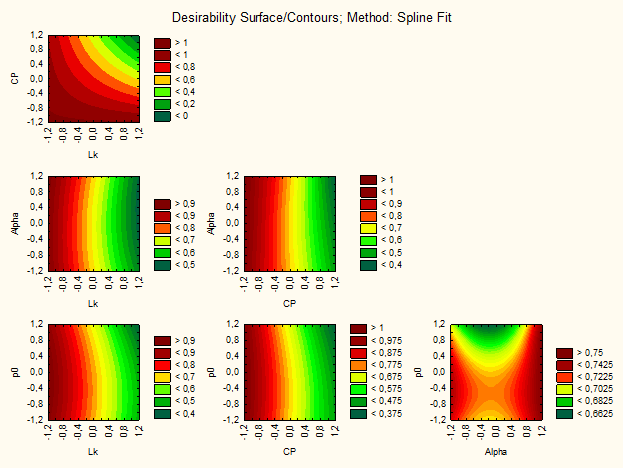
\includegraphics[width=1\textwidth]{P2M2_GV_tempo_DSC}
\end{figure}



\chapter{Imagens}
\label{chp:imagens}

\newpage

\section{Problema de \textit{Makespan}}

\begin{figure}[H]
	\centering
	\begin{subfigure}{0.49\textwidth}
	\centering
		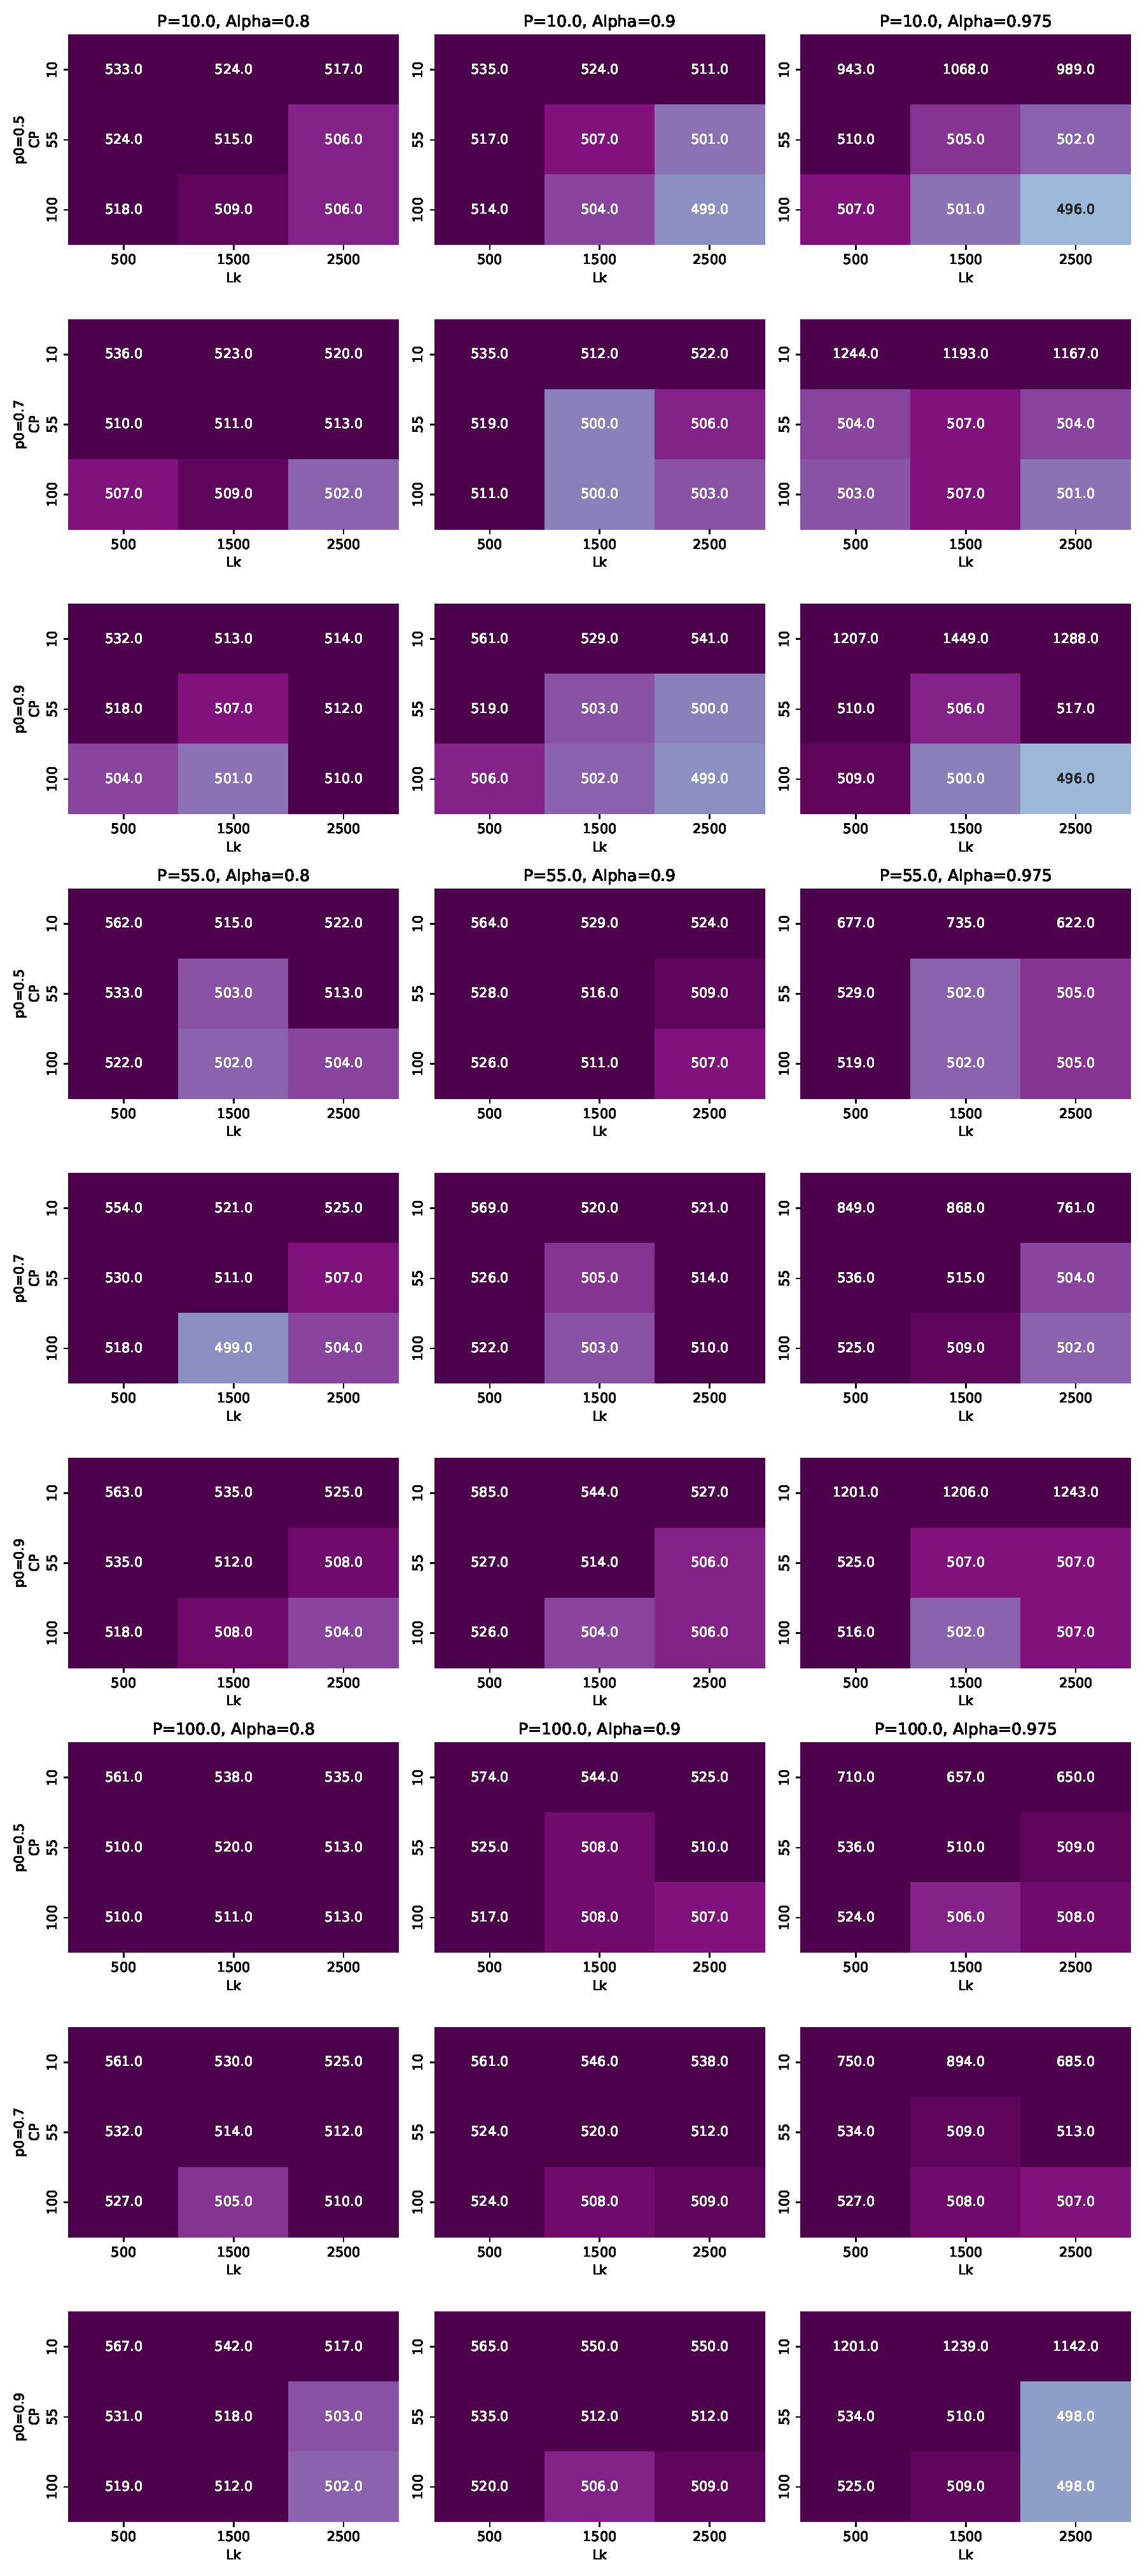
\includegraphics[width = \textwidth]{P1M1_NGV_best}
		\caption{Melhor \textit{makespan}}
		\label{fig:P1M1_NGV_best}
	\end{subfigure}
	\begin{subfigure}{0.49\textwidth}
	\centering
		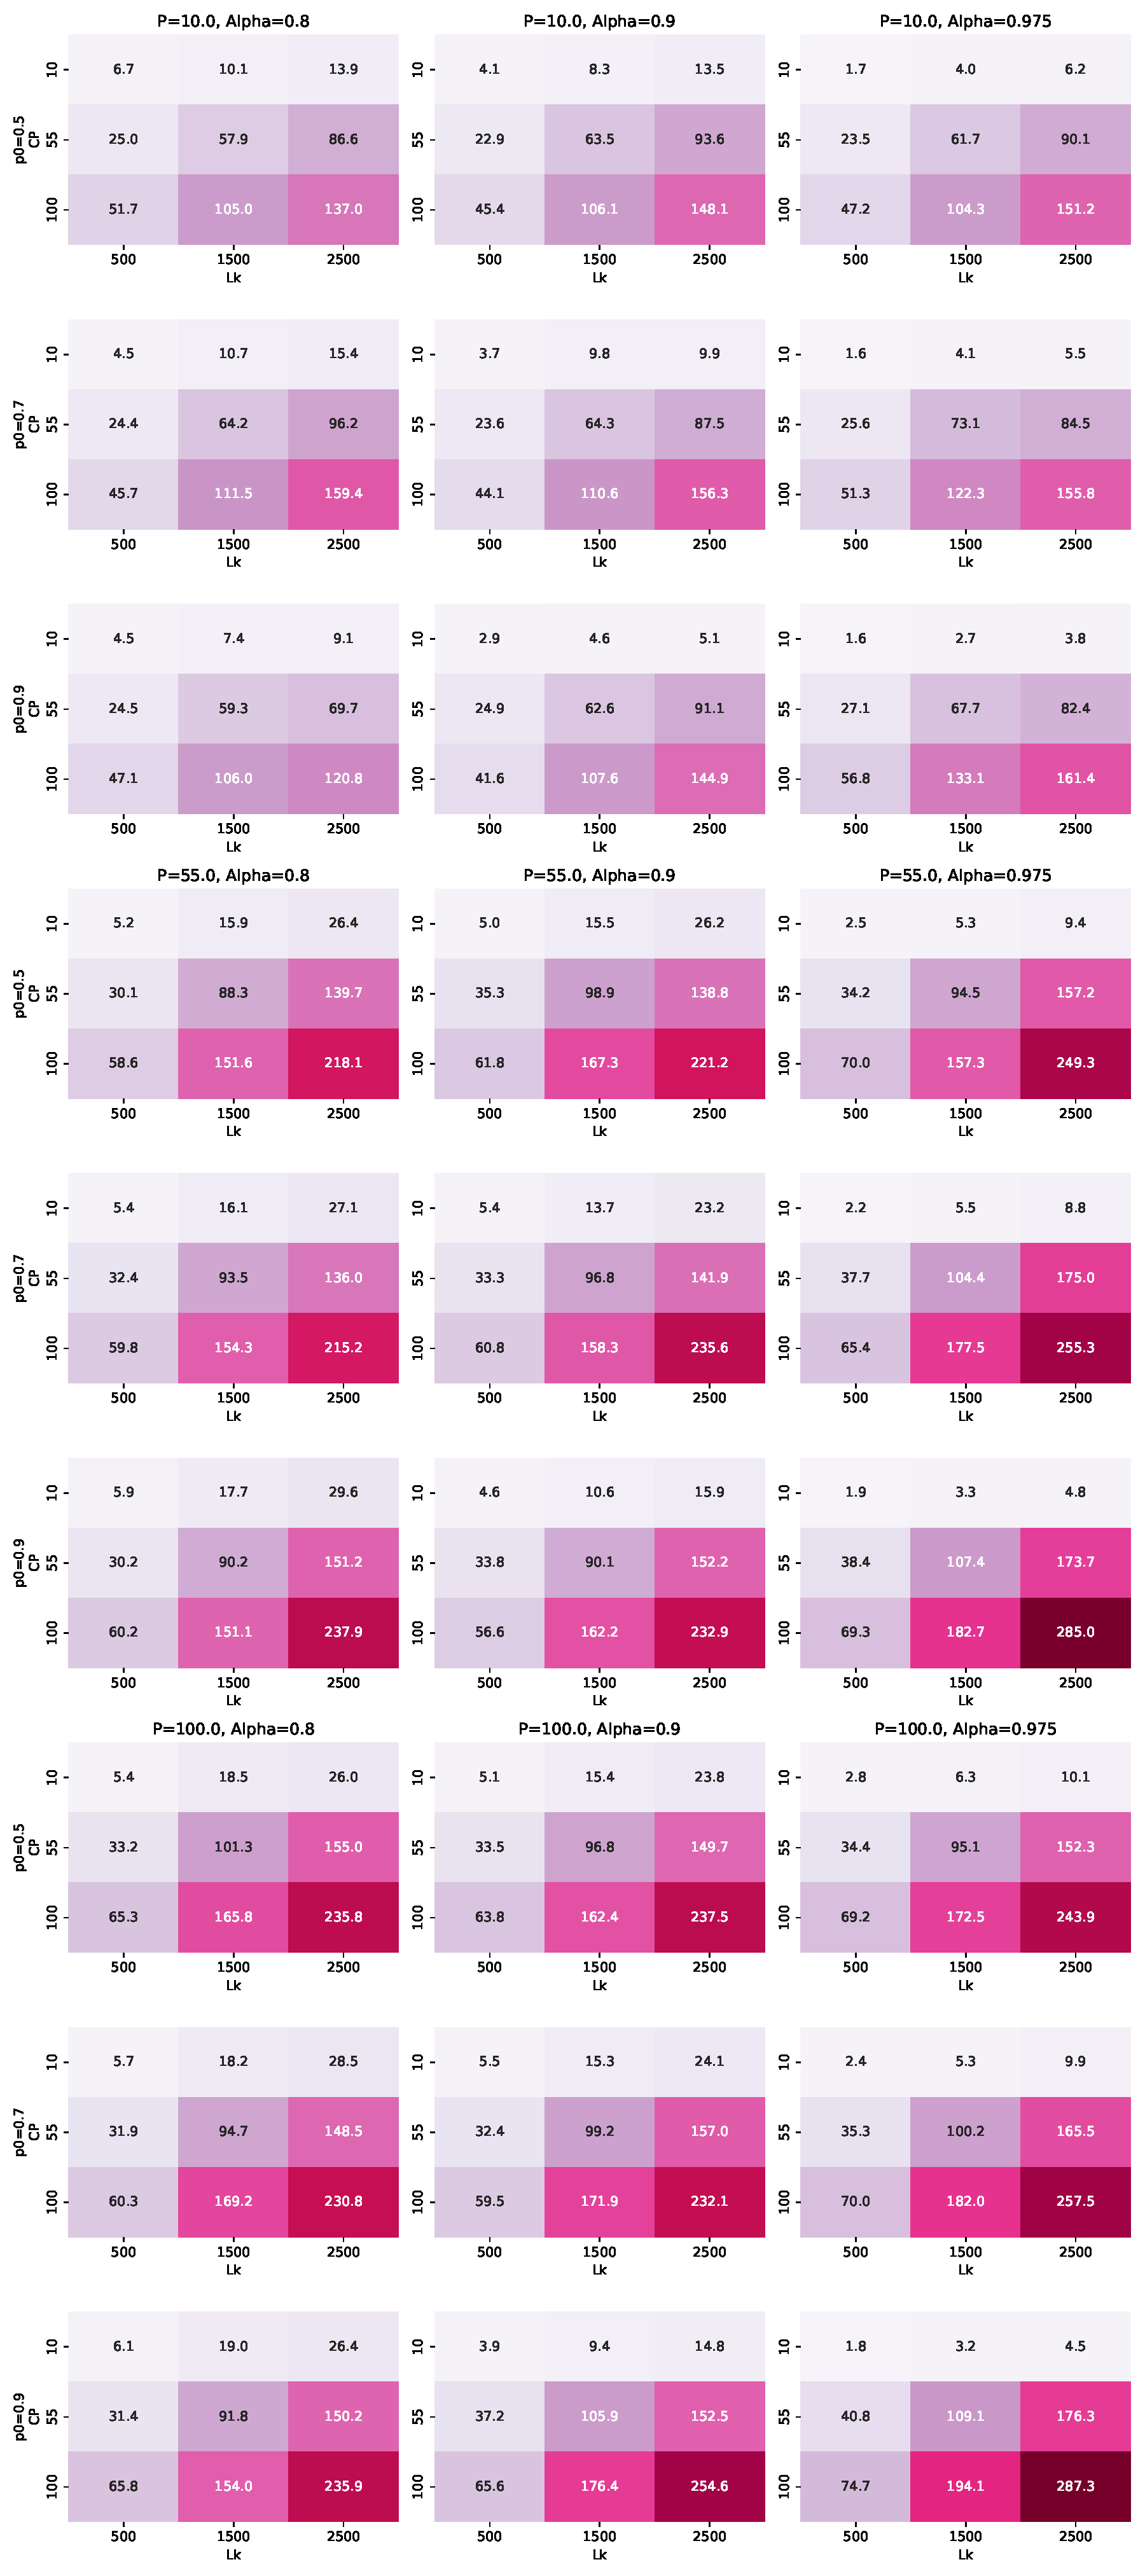
\includegraphics[width = \textwidth]{P1M1_NGV_runtime}
		\caption{Tempo de computação total}
		\label{fig:P1M1_NGV_runtime}
	\end{subfigure}
	\caption{Impacto dos níveis das variáveis sobre o valor da função objetivo e do tempo computacional para o Modelo 1 do problema de \textit{makespan}.}
	\label{fig:P1M1_NGV_alt}
\end{figure}

\begin{figure}[H]
	\centering
	\begin{subfigure}{0.49\textwidth}
	\centering
		\includegraphics[width = \textwidth]{P1M1_GV_best}
		\caption{Melhor \textit{makespan}}
		\label{fig:P1M1_GV_best}
	\end{subfigure}
	\begin{subfigure}{0.49\textwidth}
	\centering
		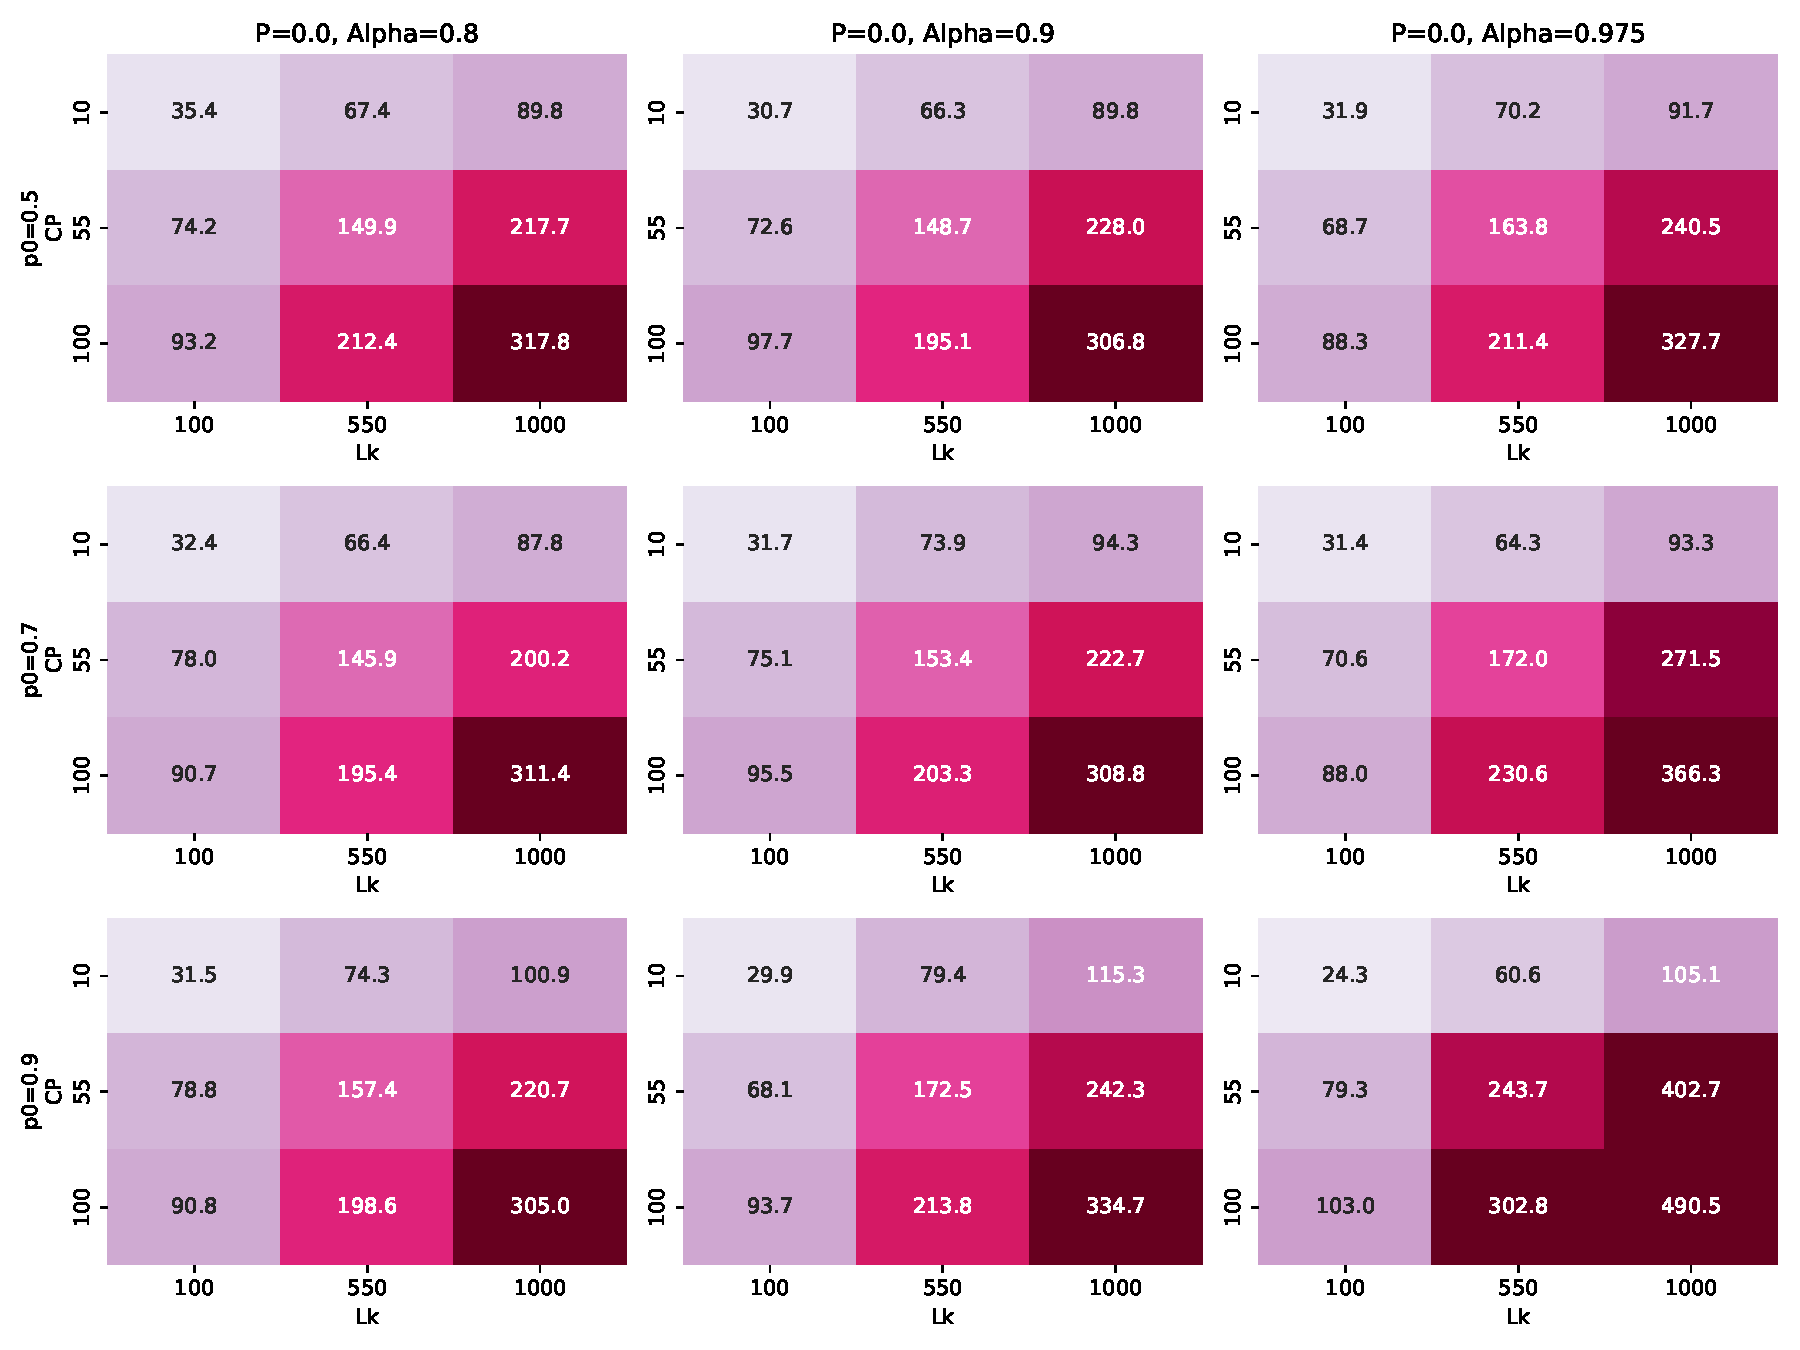
\includegraphics[width = \textwidth]{P1M1_GV_runtime}
		\caption{Tempo de computação total}
		\label{fig:P1M1_GV_runtime}
	\end{subfigure}
	\caption{Impacto dos níveis das variáveis sobre o valor da função objetivo e do tempo computacional para o Modelo 2 do problema de \textit{makespan}.}
	\label{fig:P1M1_GV_alt}
\end{figure}

\begin{figure}[H]
	\centering
	\begin{subfigure}{0.49\textwidth}
	\centering
		\includegraphics[width = \textwidth]{P1M2_GV_best}
		\caption{Melhor \textit{makespan}}
		\label{fig:P1M2_GV_best}
	\end{subfigure}
	\begin{subfigure}{0.49\textwidth}
	\centering
		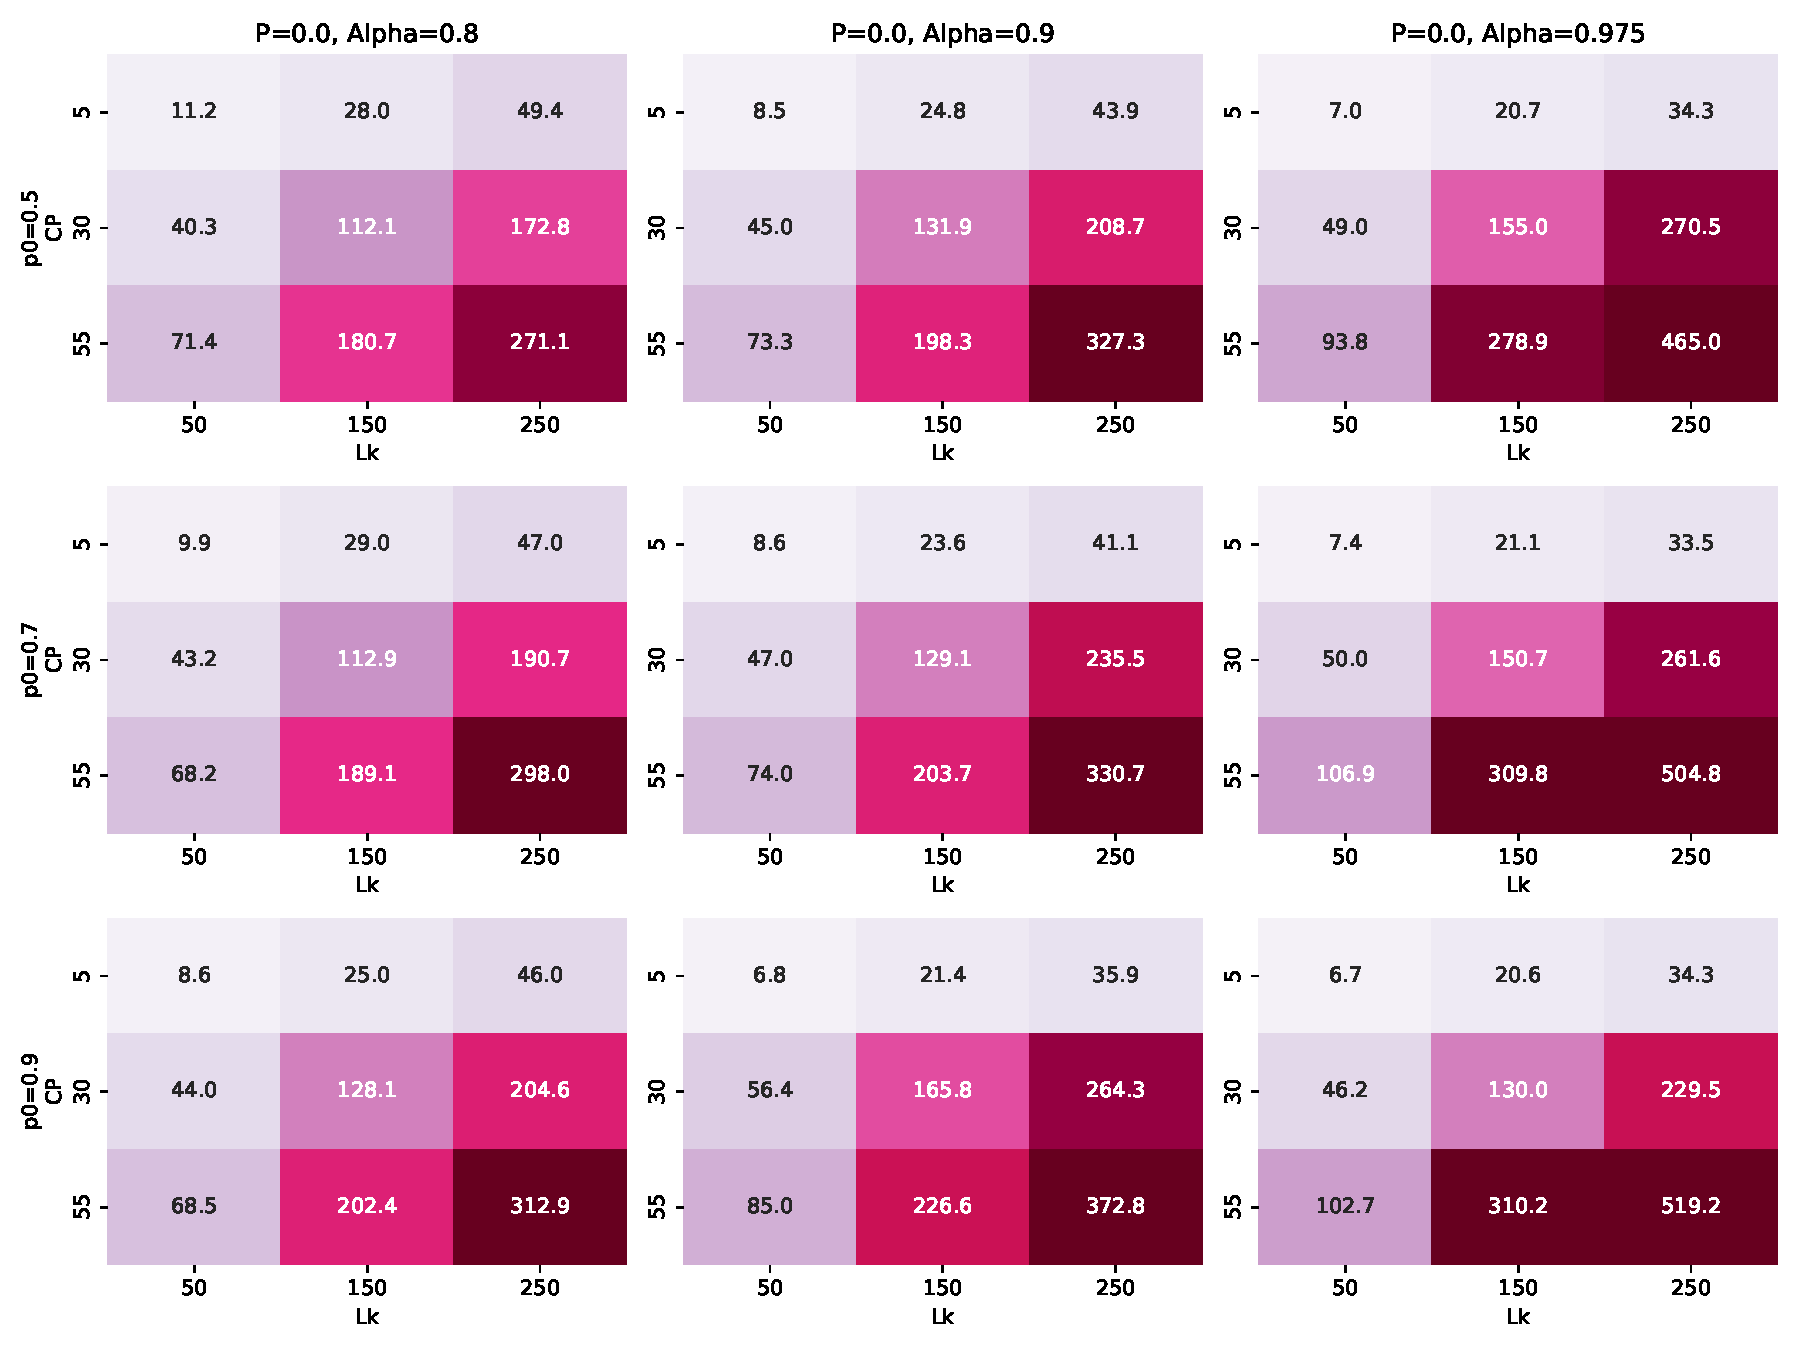
\includegraphics[width = \textwidth]{P1M2_GV_runtime}
		\caption{Tempo de computação total}
		\label{fig:P1M2_GV_runtime}
	\end{subfigure}
	\caption{Impacto dos níveis das variáveis sobre o valor da função objetivo e do tempo computacional para o Modelo 3 com \textit{left shifting} do problema de \textit{makespan}.}
	\label{fig:P1M2_GV_alt}
\end{figure}

\begin{figure}[H]
	\centering
	\begin{subfigure}{0.49\textwidth}
	\centering
		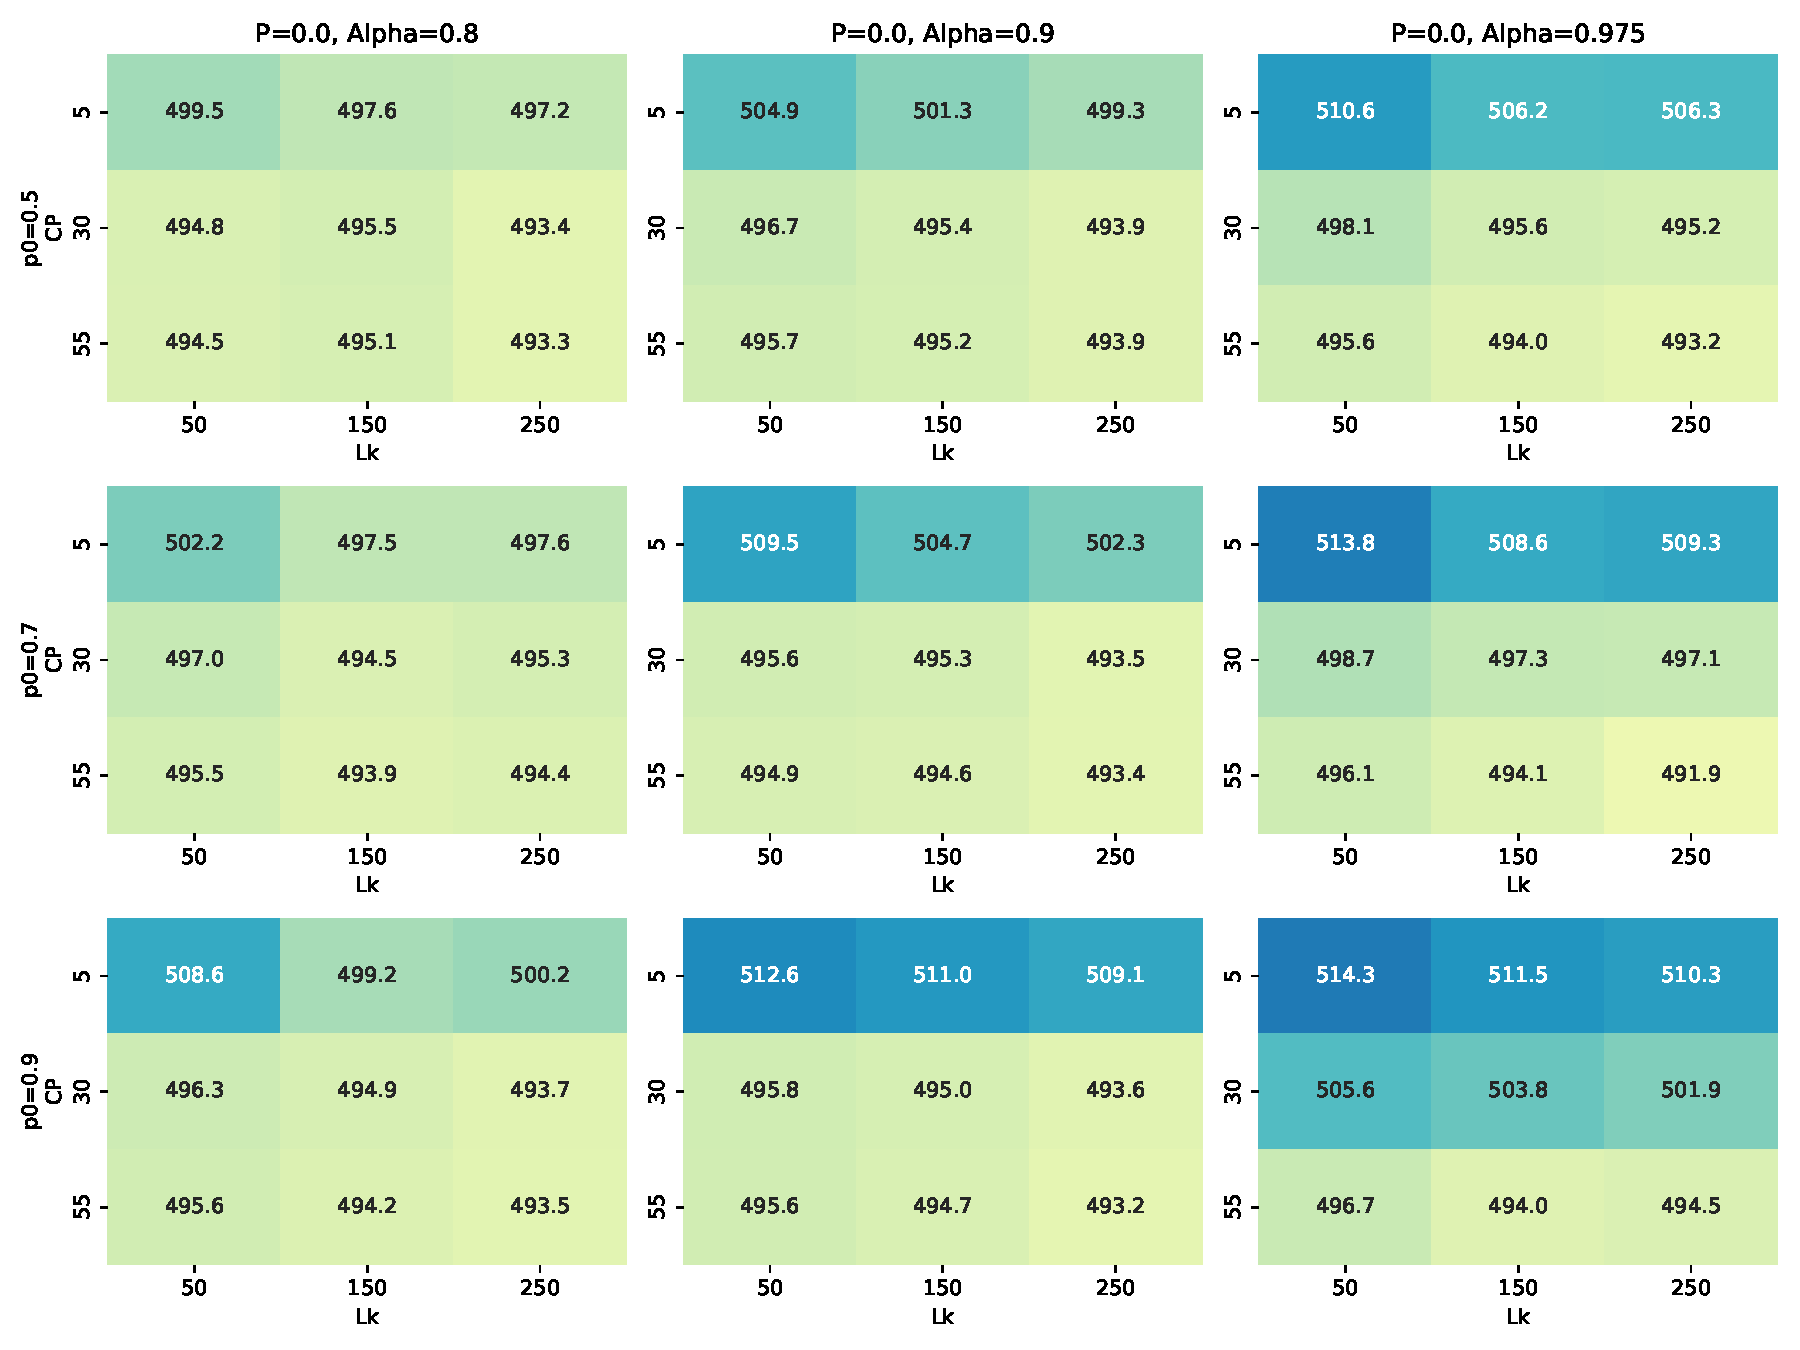
\includegraphics[width = \textwidth]{P1M2_GV_REVTT_objf}
		\caption{Média do mínimo de \textit{makespan}}
		\label{fig:P1M2_GV_REVTT_objf}
	\end{subfigure}
	\begin{subfigure}{0.49\textwidth}
	\centering
		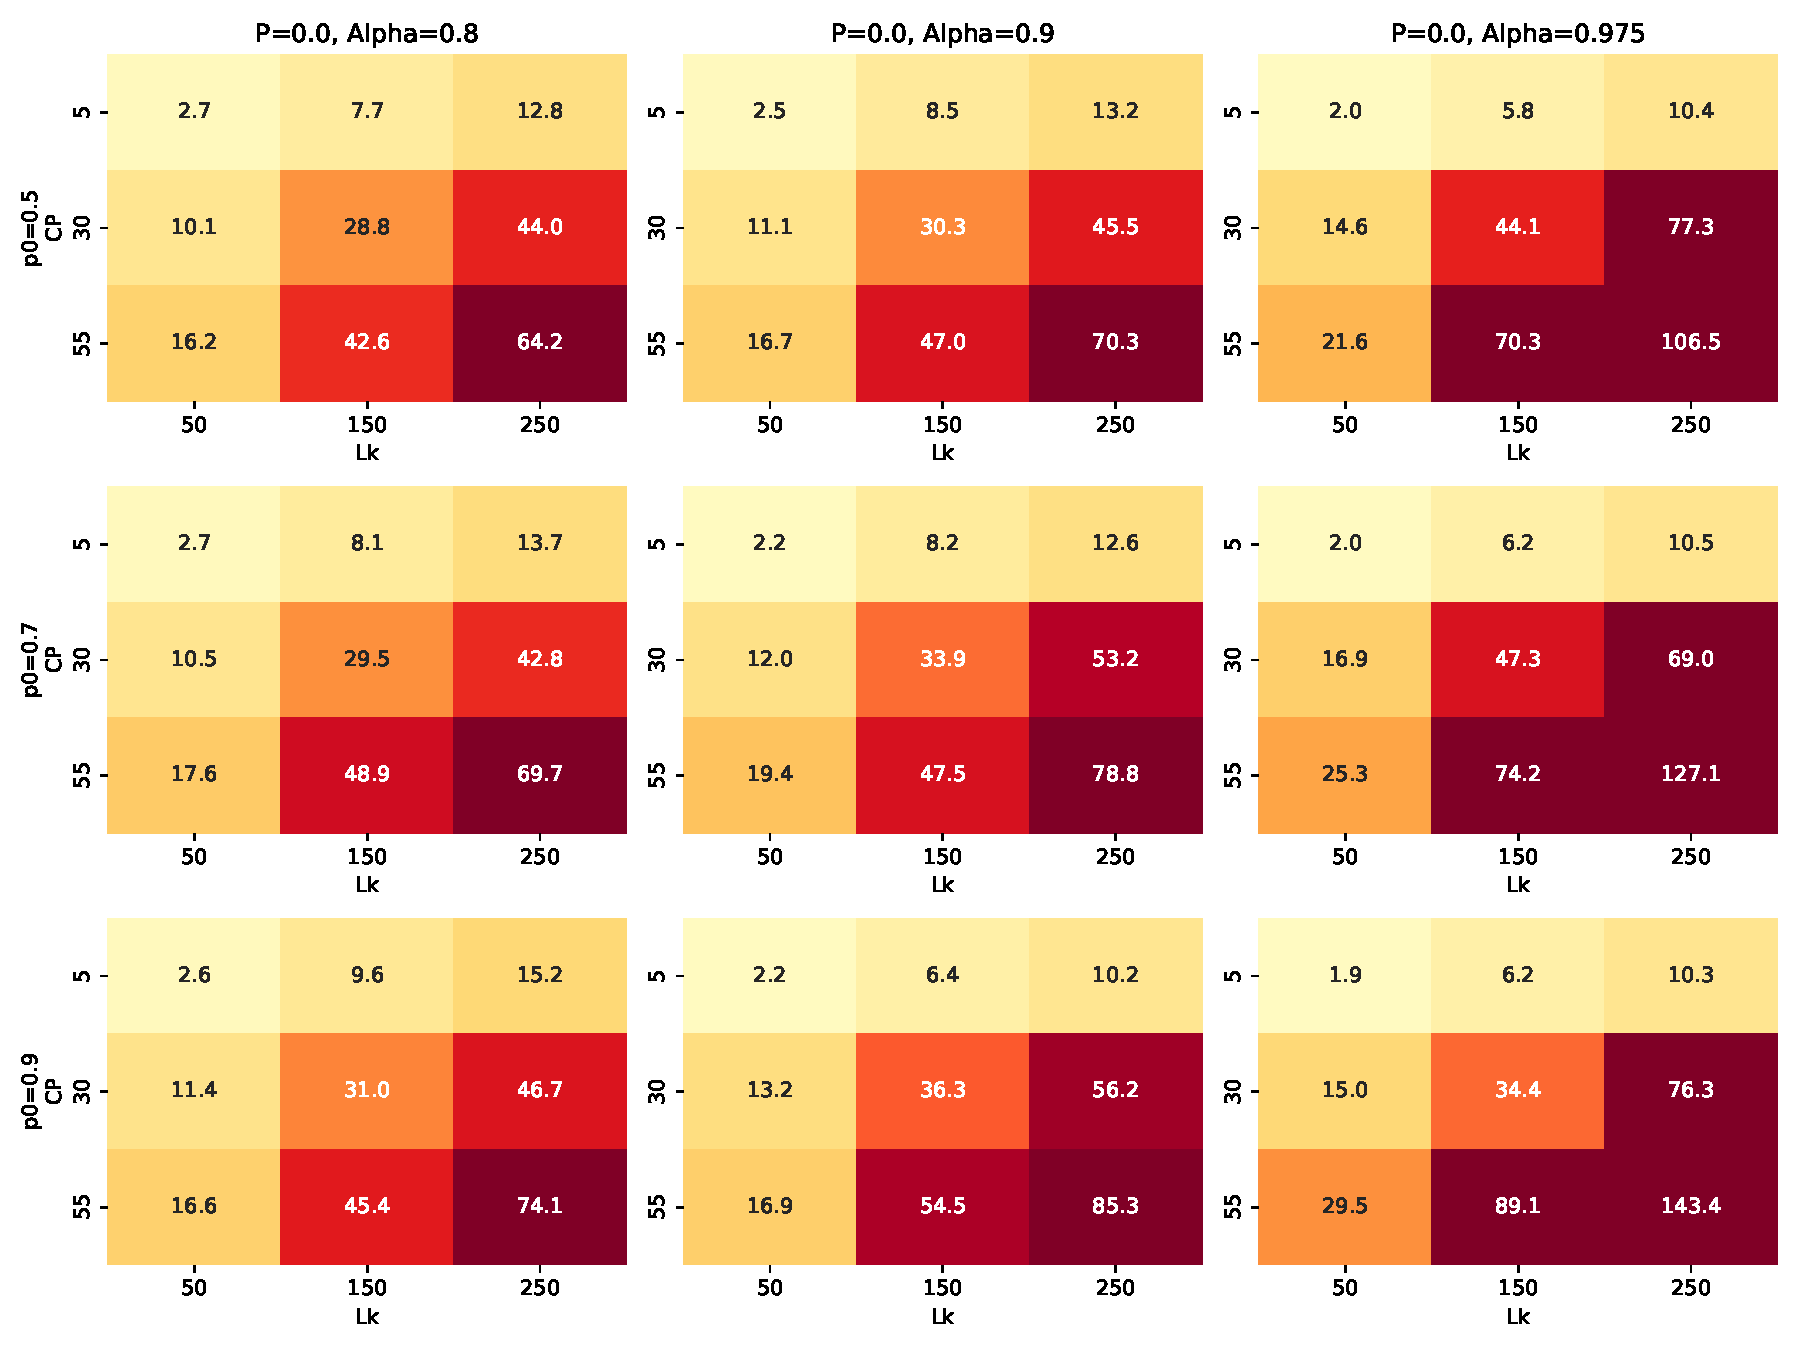
\includegraphics[width = \textwidth]{P1M2_GV_REVTT_time}
		\caption{Média do máximo do tempo de computação}
		\label{fig:P1M2_GV_REVTT_time}
	\end{subfigure}
	\label{fig:P1M2_GV_REVTT_alt}
	\centering
	\begin{subfigure}{0.49\textwidth}
	\centering
		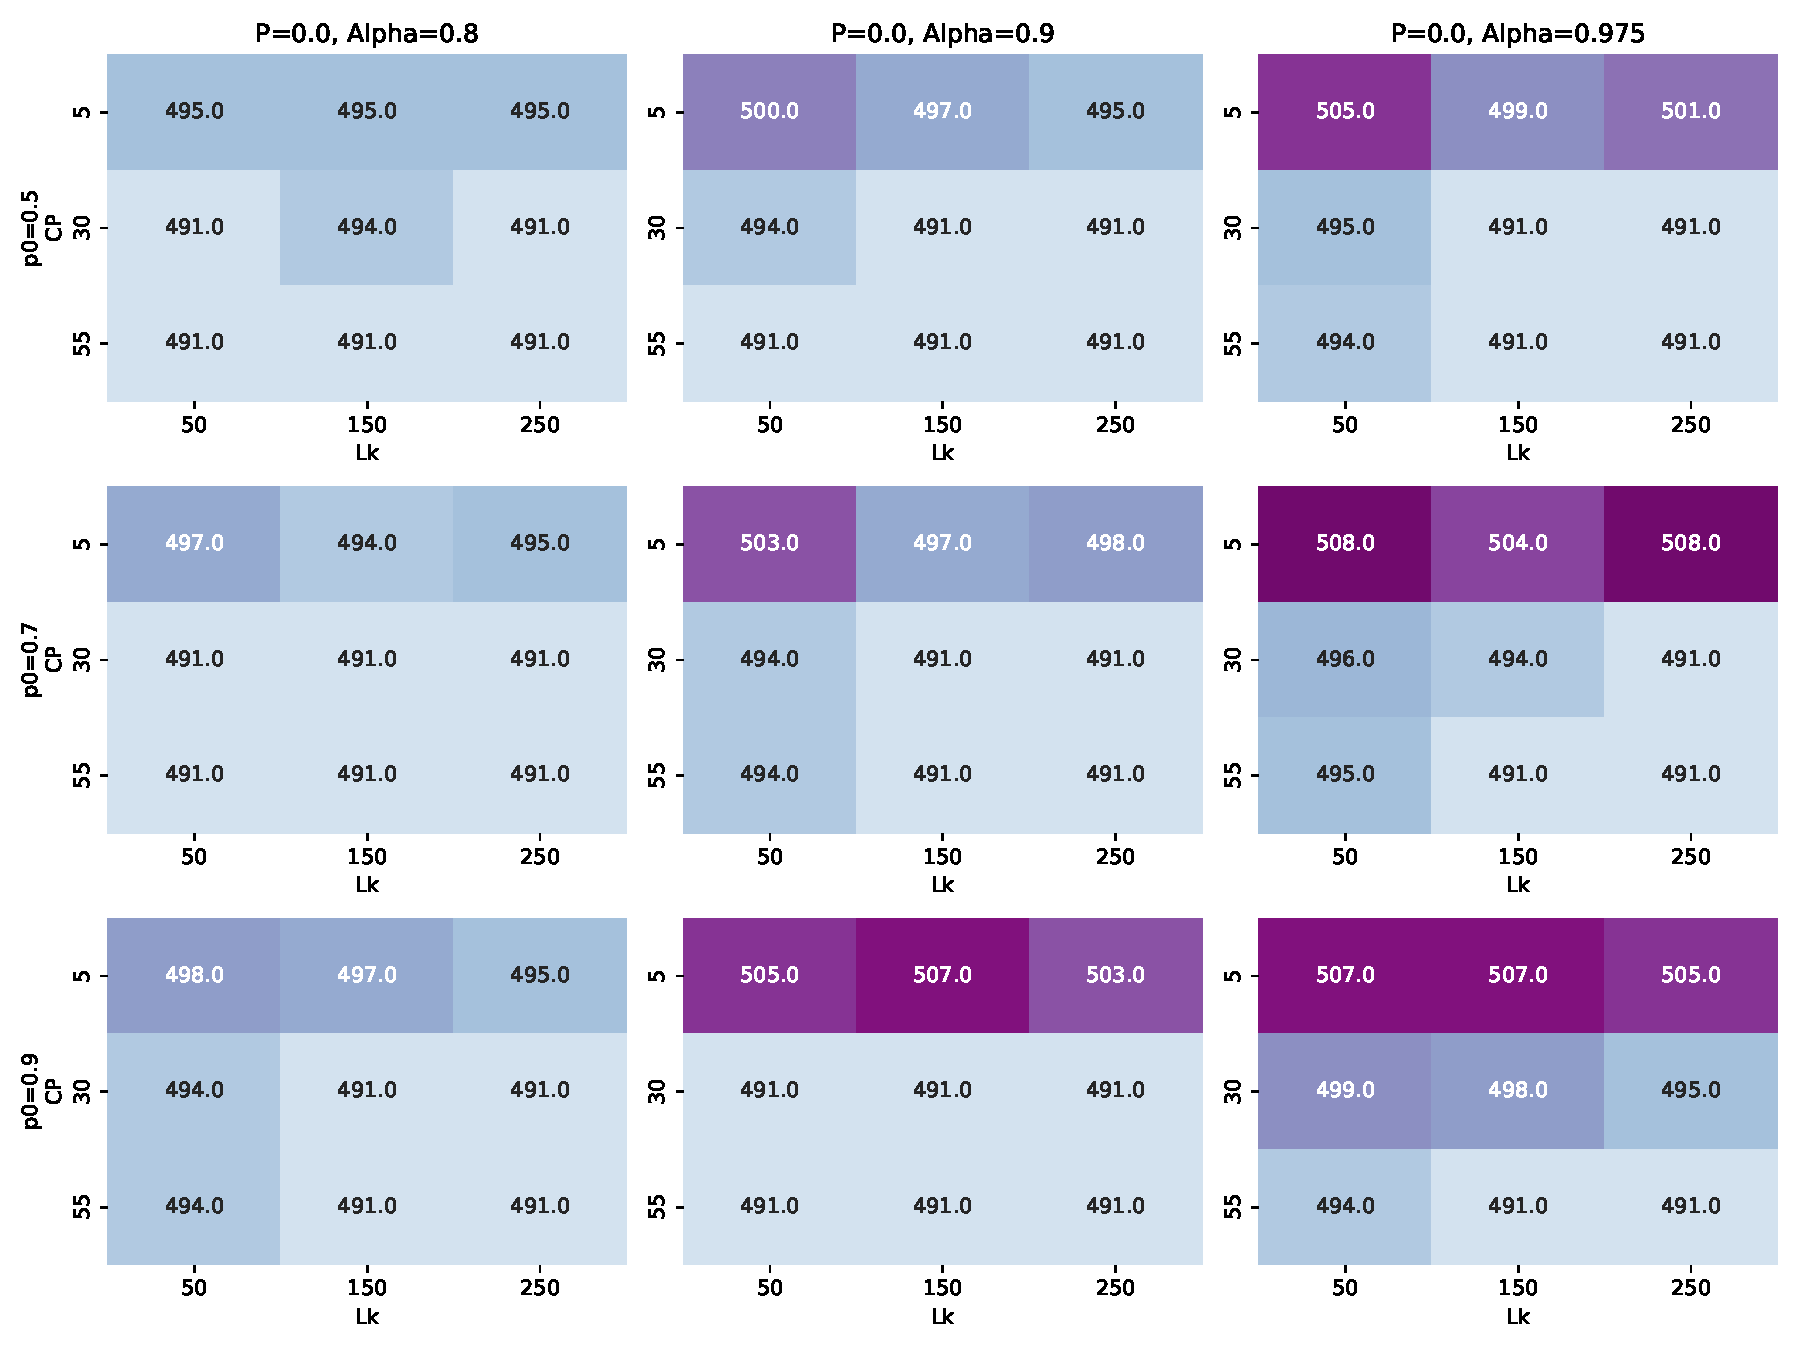
\includegraphics[width = \textwidth]{P1M2_GV_REVTT_best}
		\caption{Melhor \textit{makespan}}
		\label{fig:P1M2_GV_REVTT_best}
	\end{subfigure}
	\begin{subfigure}{0.49\textwidth}
	\centering
		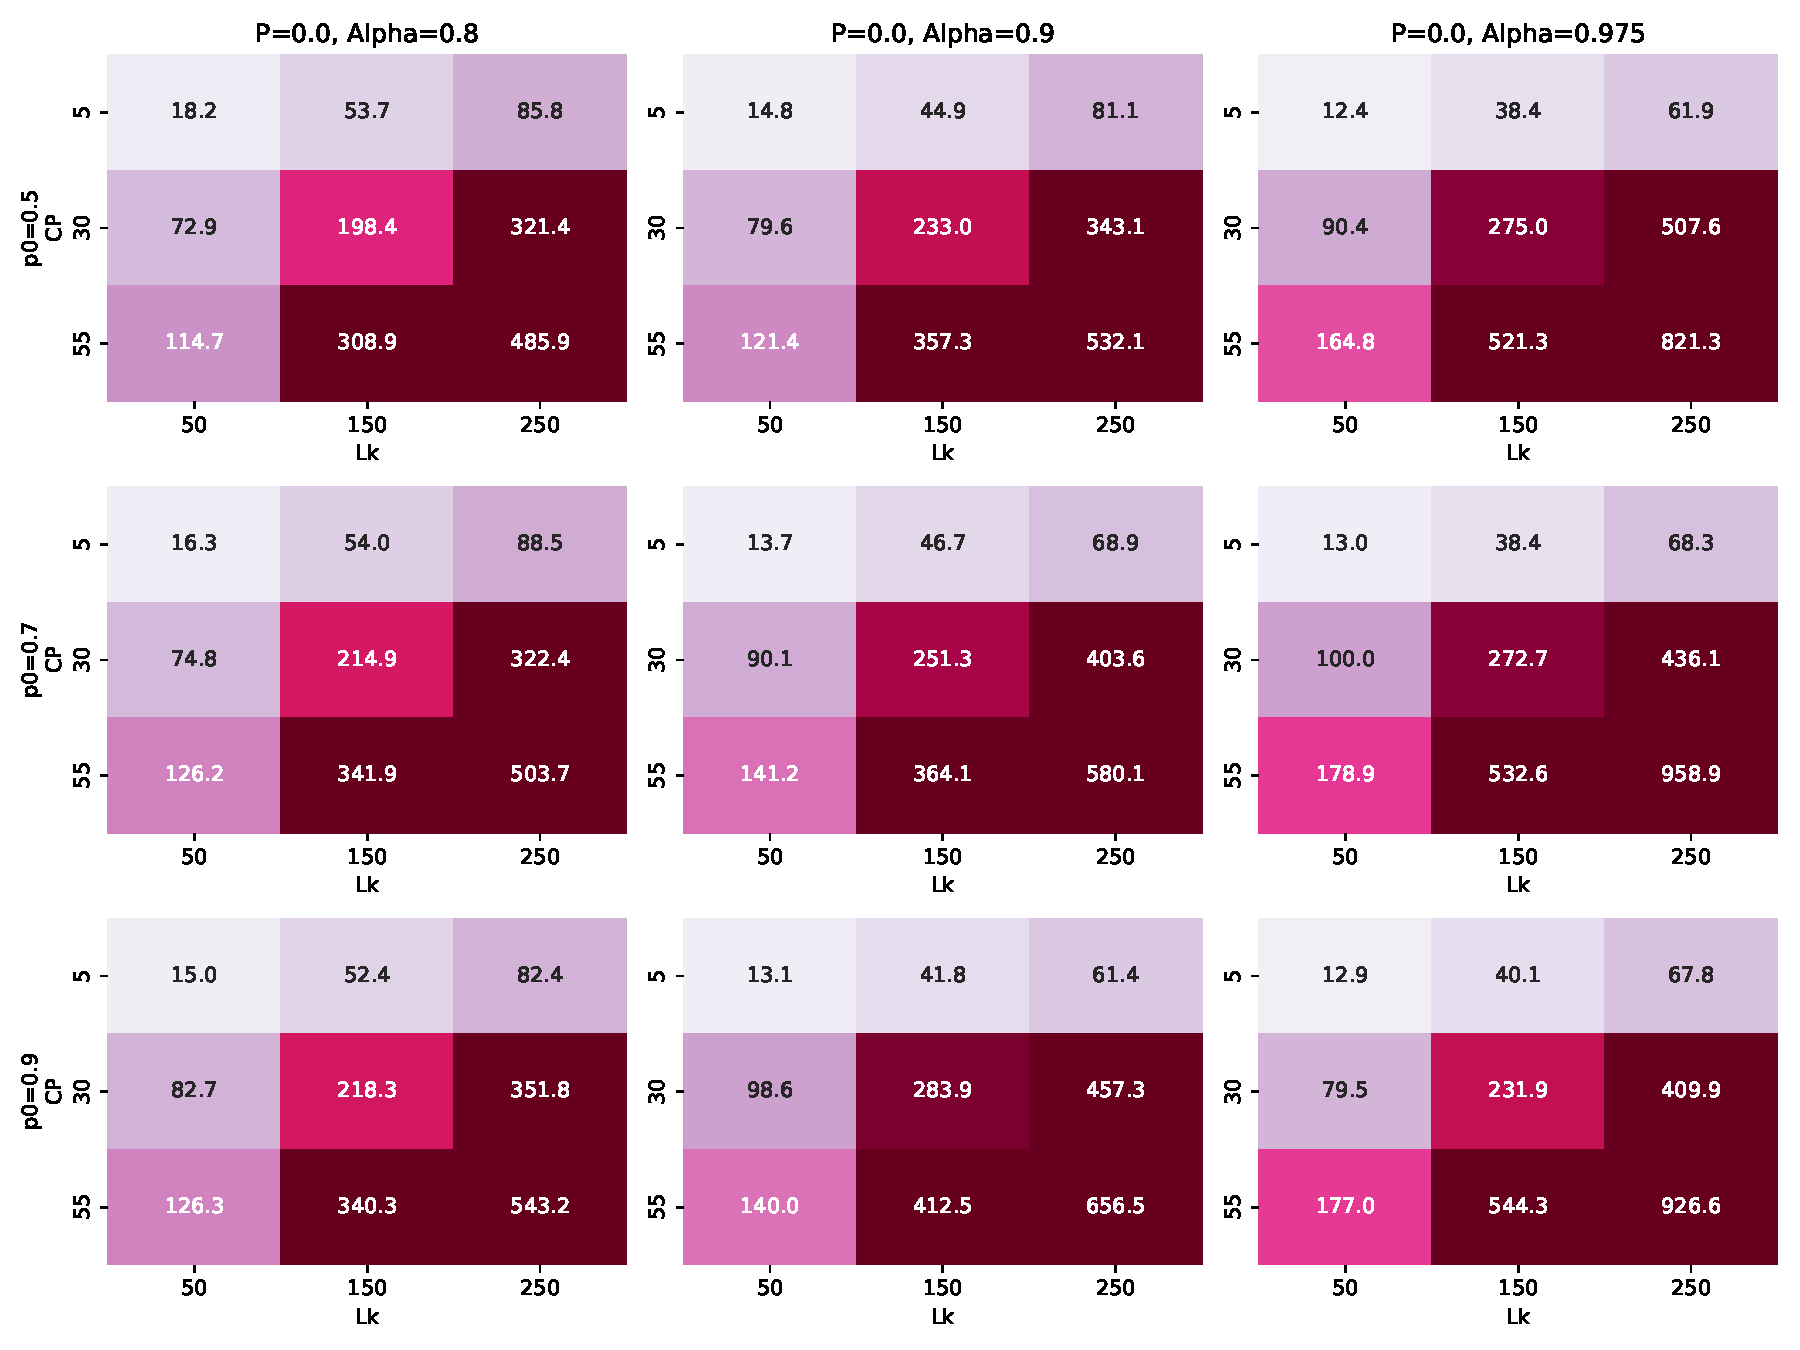
\includegraphics[width = \textwidth]{P1M2_GV_REVTT_runtime}
		\caption{Tempo de computação total}
		\label{fig:P1M2_GV_REVTT_runtime}
	\end{subfigure}
	\caption{Impacto dos níveis das variáveis sobre o valor da função objetivo e do tempo computacional para o Modelo 3 com \textit{enhanced left shifting} do problema de \textit{makespan}.}
	\label{fig:P1M2_GV_REVTT_alt}
\end{figure}

\begin{figure}[H]
	\centering
	\begin{subfigure}{0.49\textwidth}
	\centering
		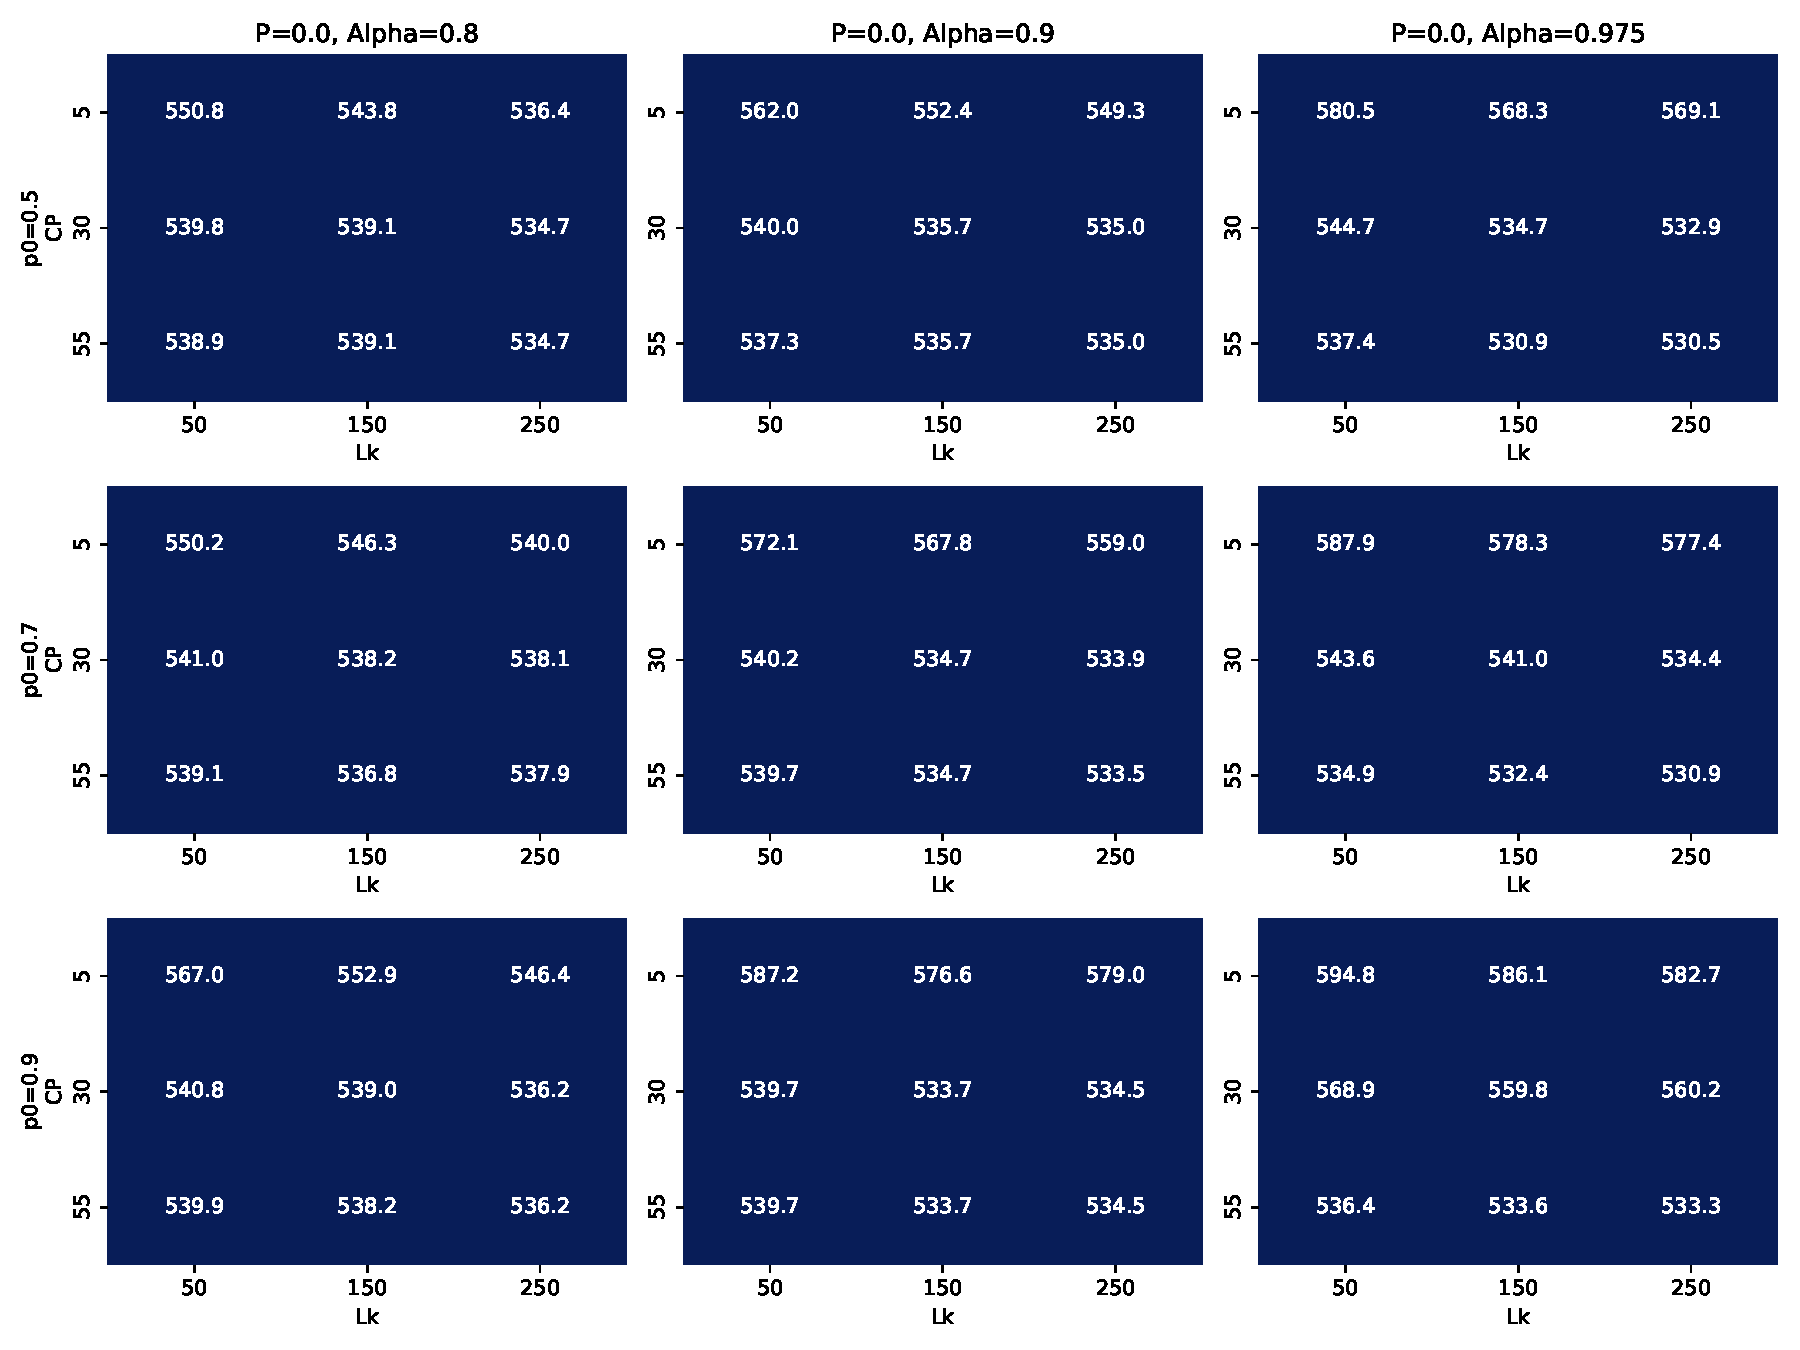
\includegraphics[width = \textwidth]{P1M2_GV_ND_objf}
		\caption{Média do mínimo de \textit{makespan}}
		\label{fig:P1M2_GV_ND_objf}
	\end{subfigure}
	\begin{subfigure}{0.49\textwidth}
	\centering
		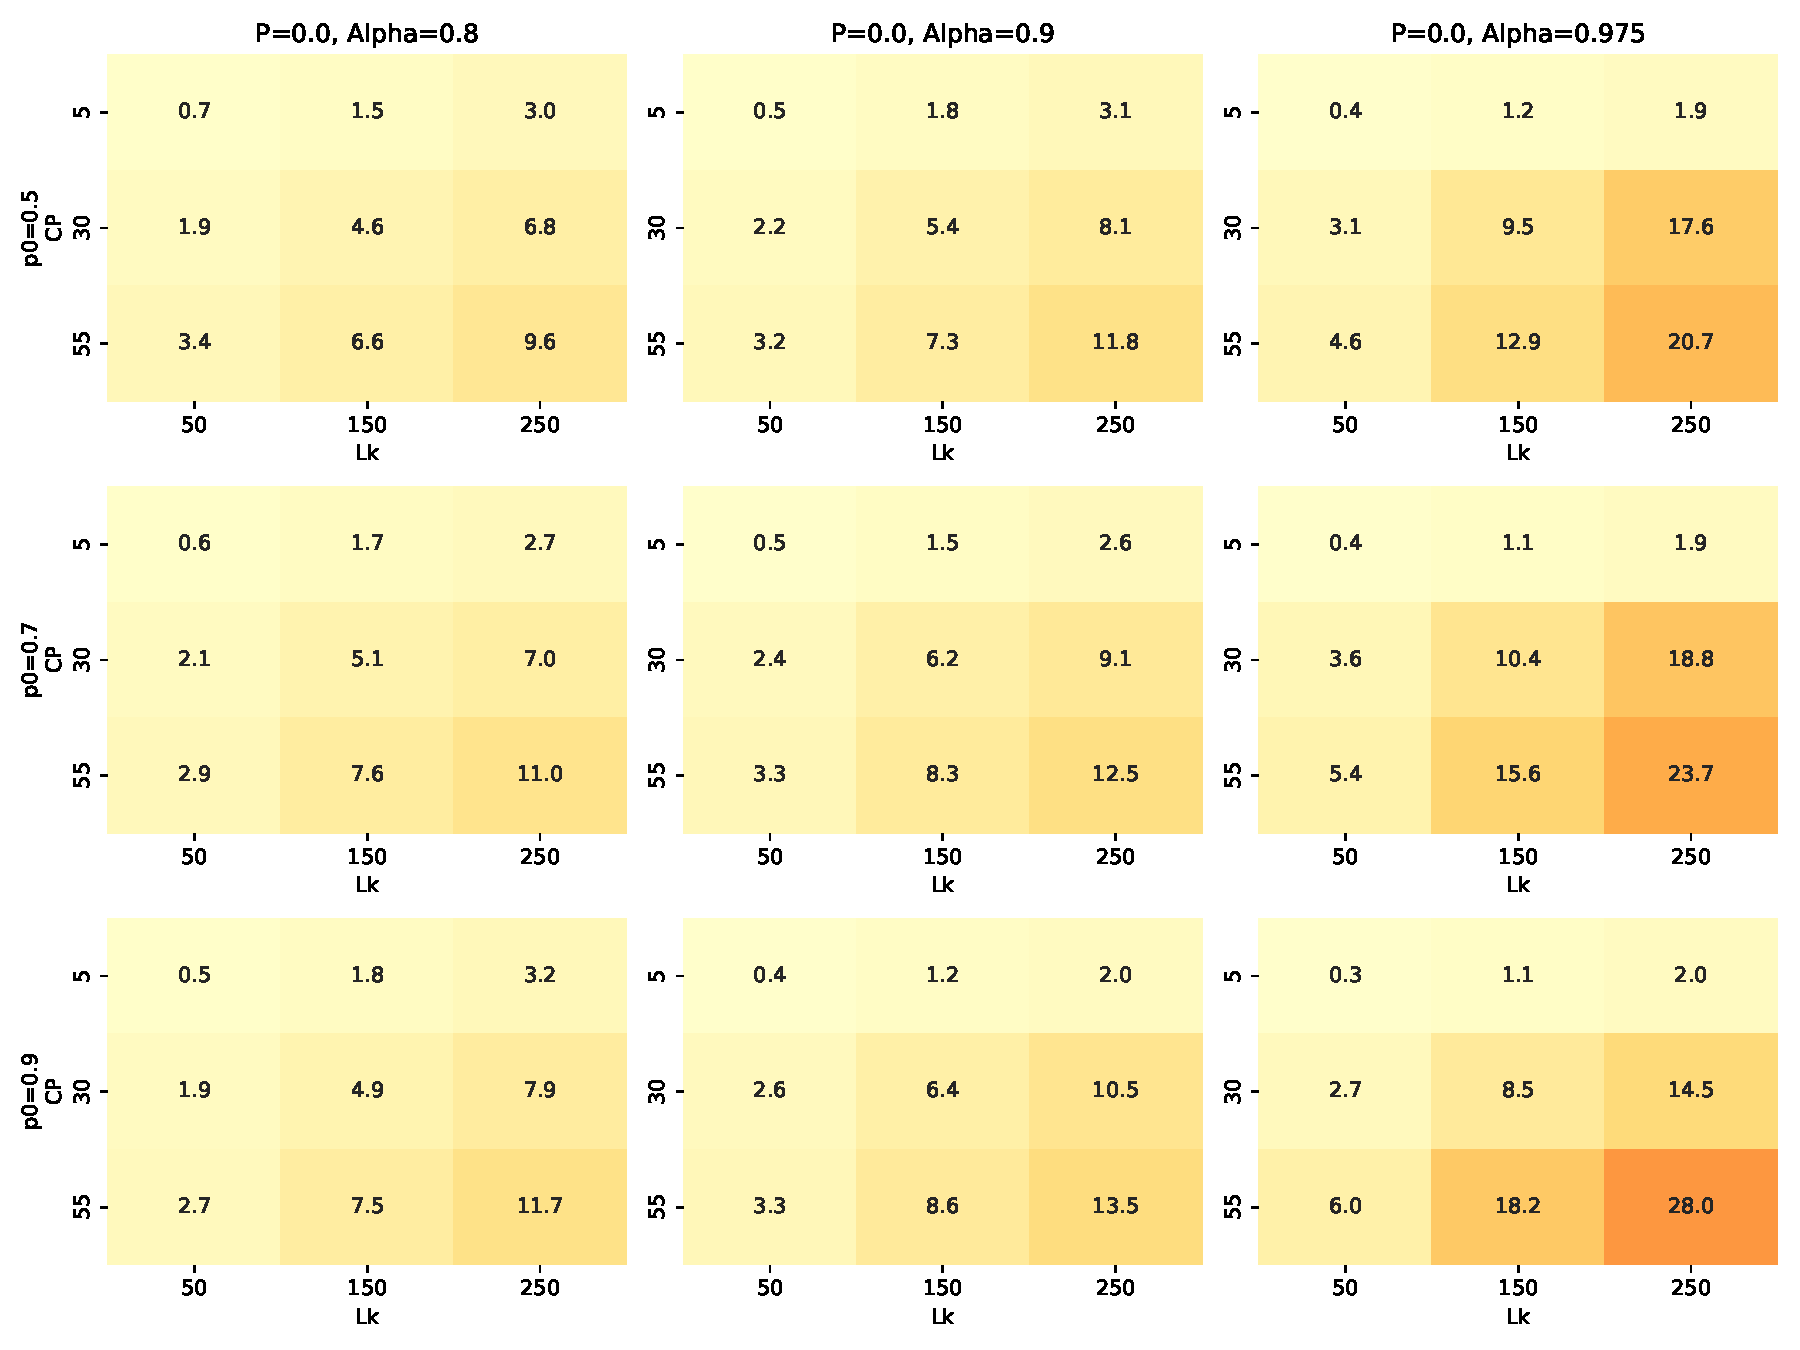
\includegraphics[width = \textwidth]{P1M2_GV_ND_time}
		\caption{Média do máximo do tempo de computação}
		\label{fig:P1M2_GV_ND_time}
	\end{subfigure}
	\label{fig:P1M2_GV_ND_alt}
	\centering
	\begin{subfigure}{0.49\textwidth}
	\centering
		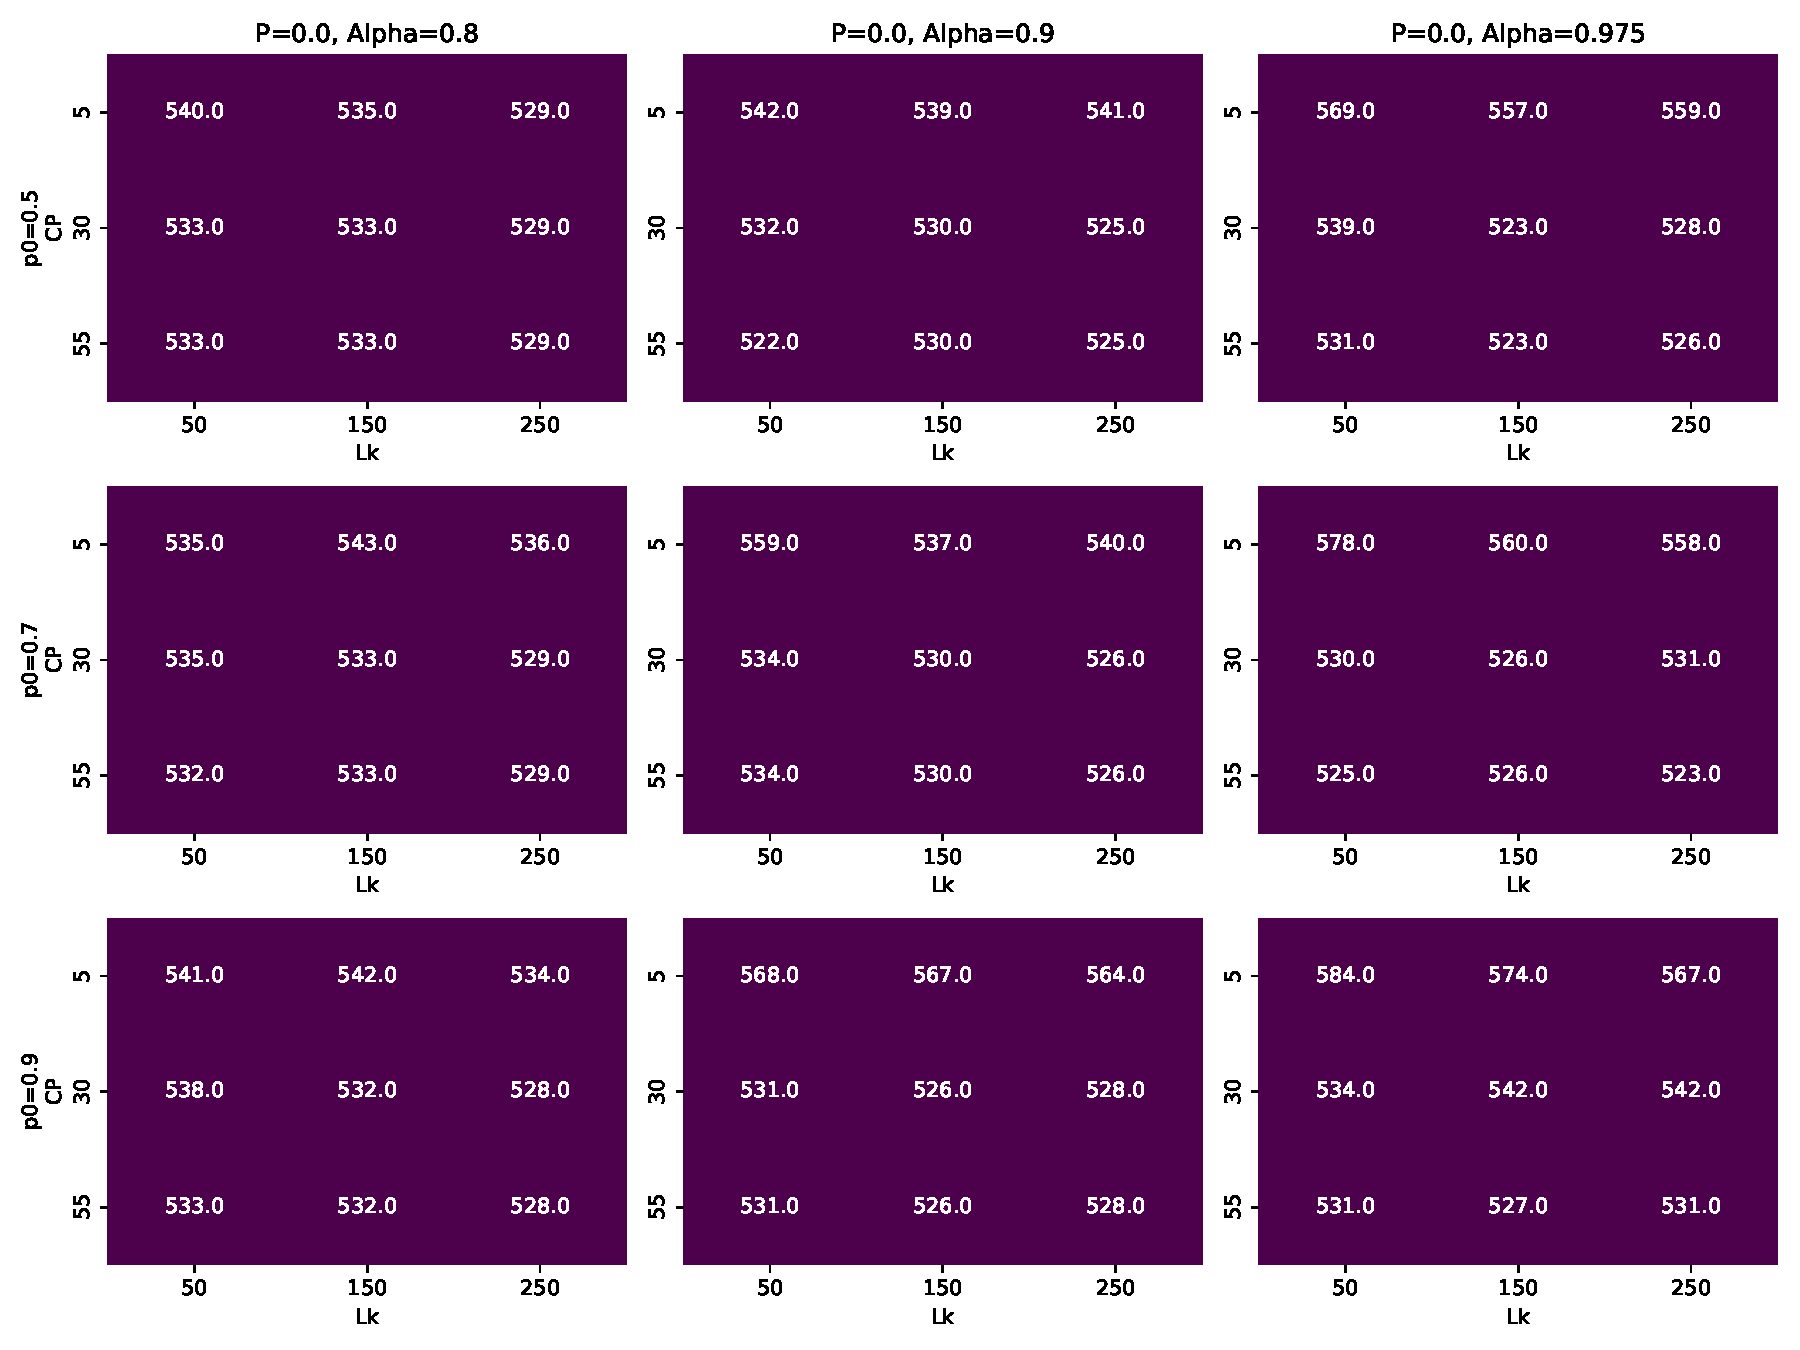
\includegraphics[width = \textwidth]{P1M2_GV_ND_best}
		\caption{Melhor \textit{makespan}}
		\label{fig:P1M2_GV_ND_best}
	\end{subfigure}
	\begin{subfigure}{0.49\textwidth}
	\centering
		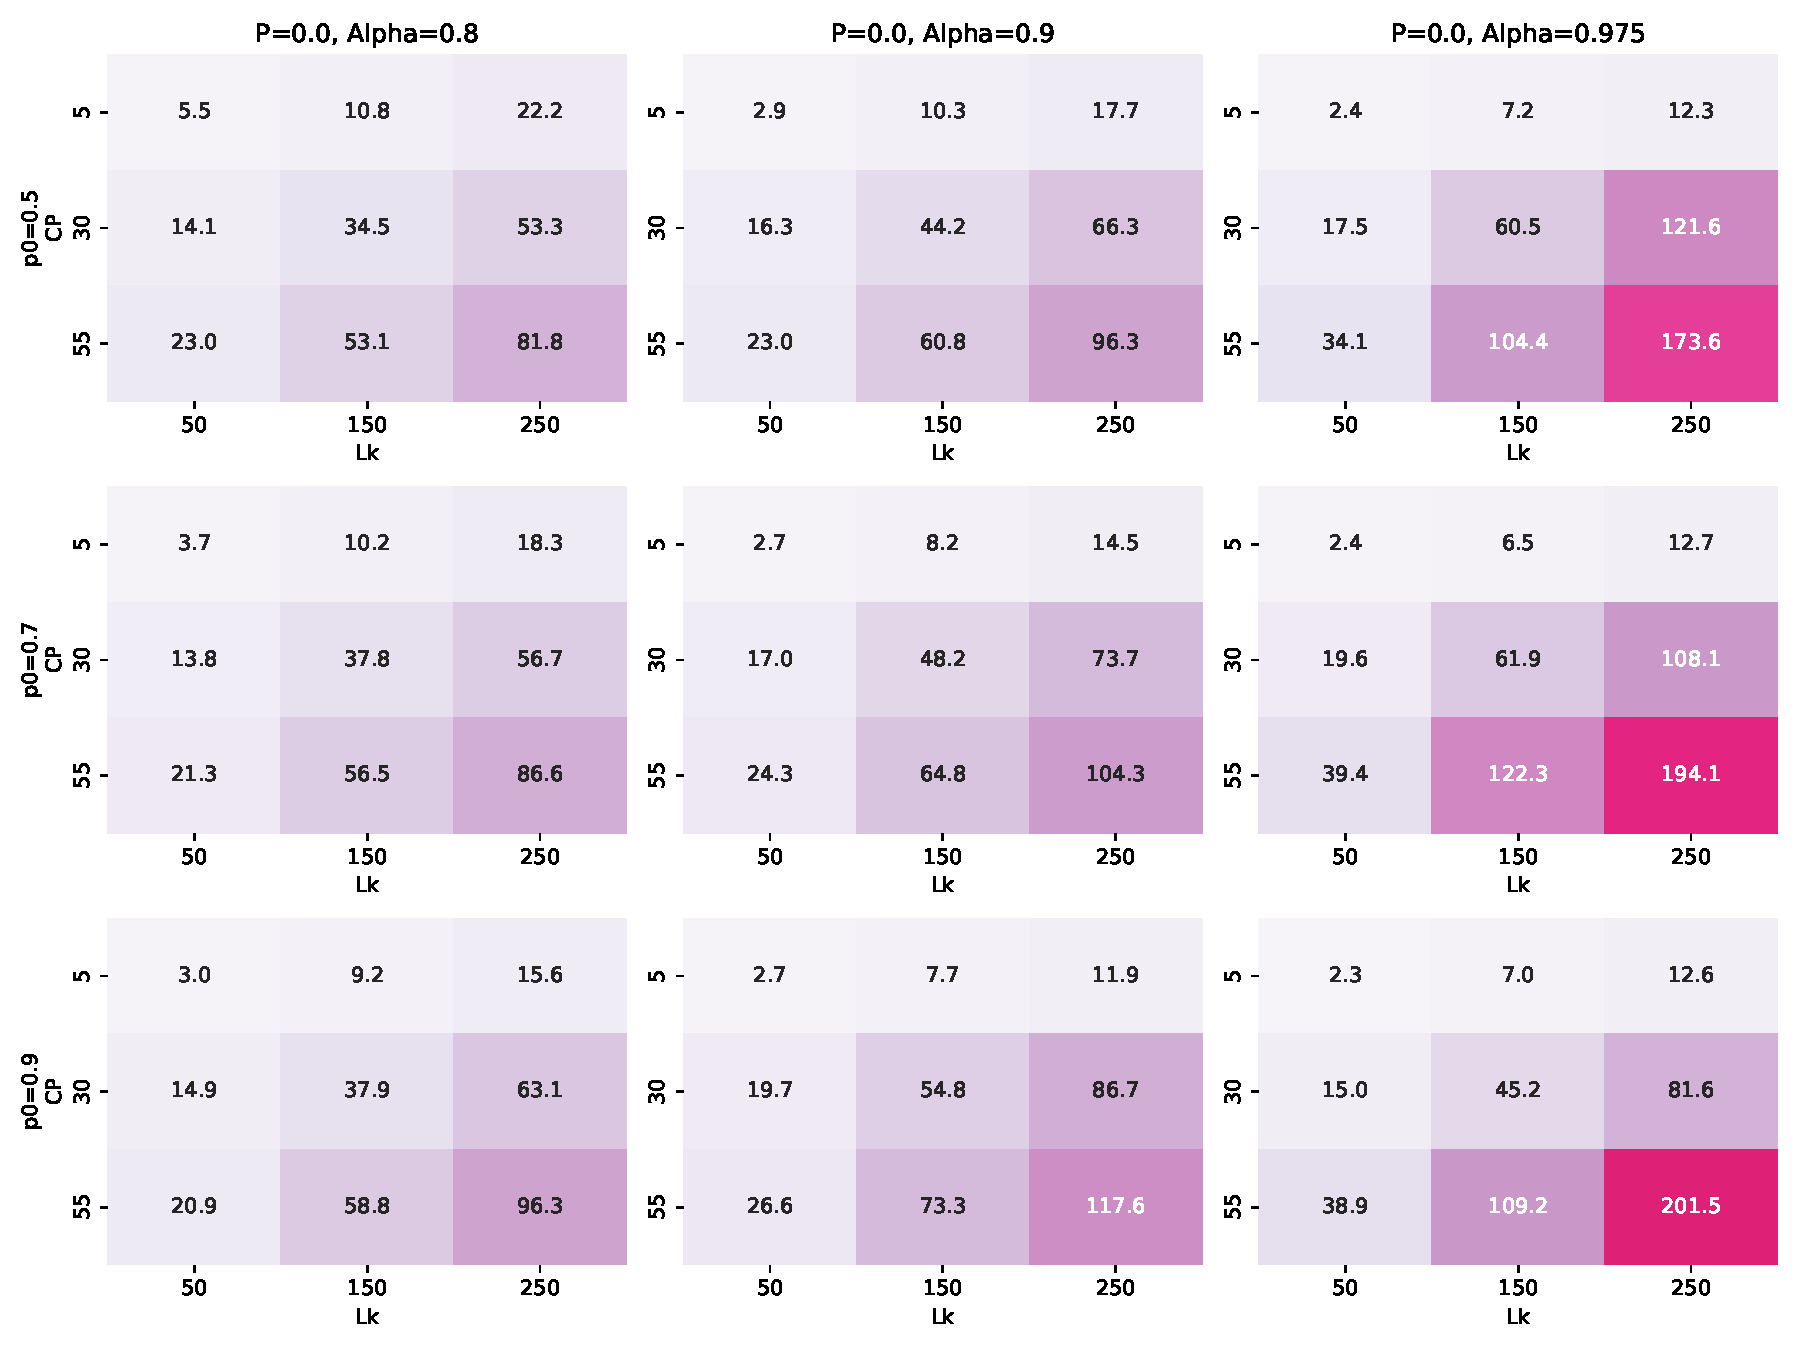
\includegraphics[width = \textwidth]{P1M2_GV_ND_runtime}
		\caption{Tempo de computação total}
		\label{fig:P1M2_GV_ND_runtime}
	\end{subfigure}
	\caption{Impacto dos níveis das variáveis sobre o valor da função objetivo e do tempo computacional para o Modelo 3 com \textit{non-delay} do problema de \textit{makespan}.}
	\label{fig:P1M2_GV_ND_alt}
\end{figure}

\begin{figure}[H]
	\centering
	\begin{subfigure}{0.49\textwidth}
	\centering
		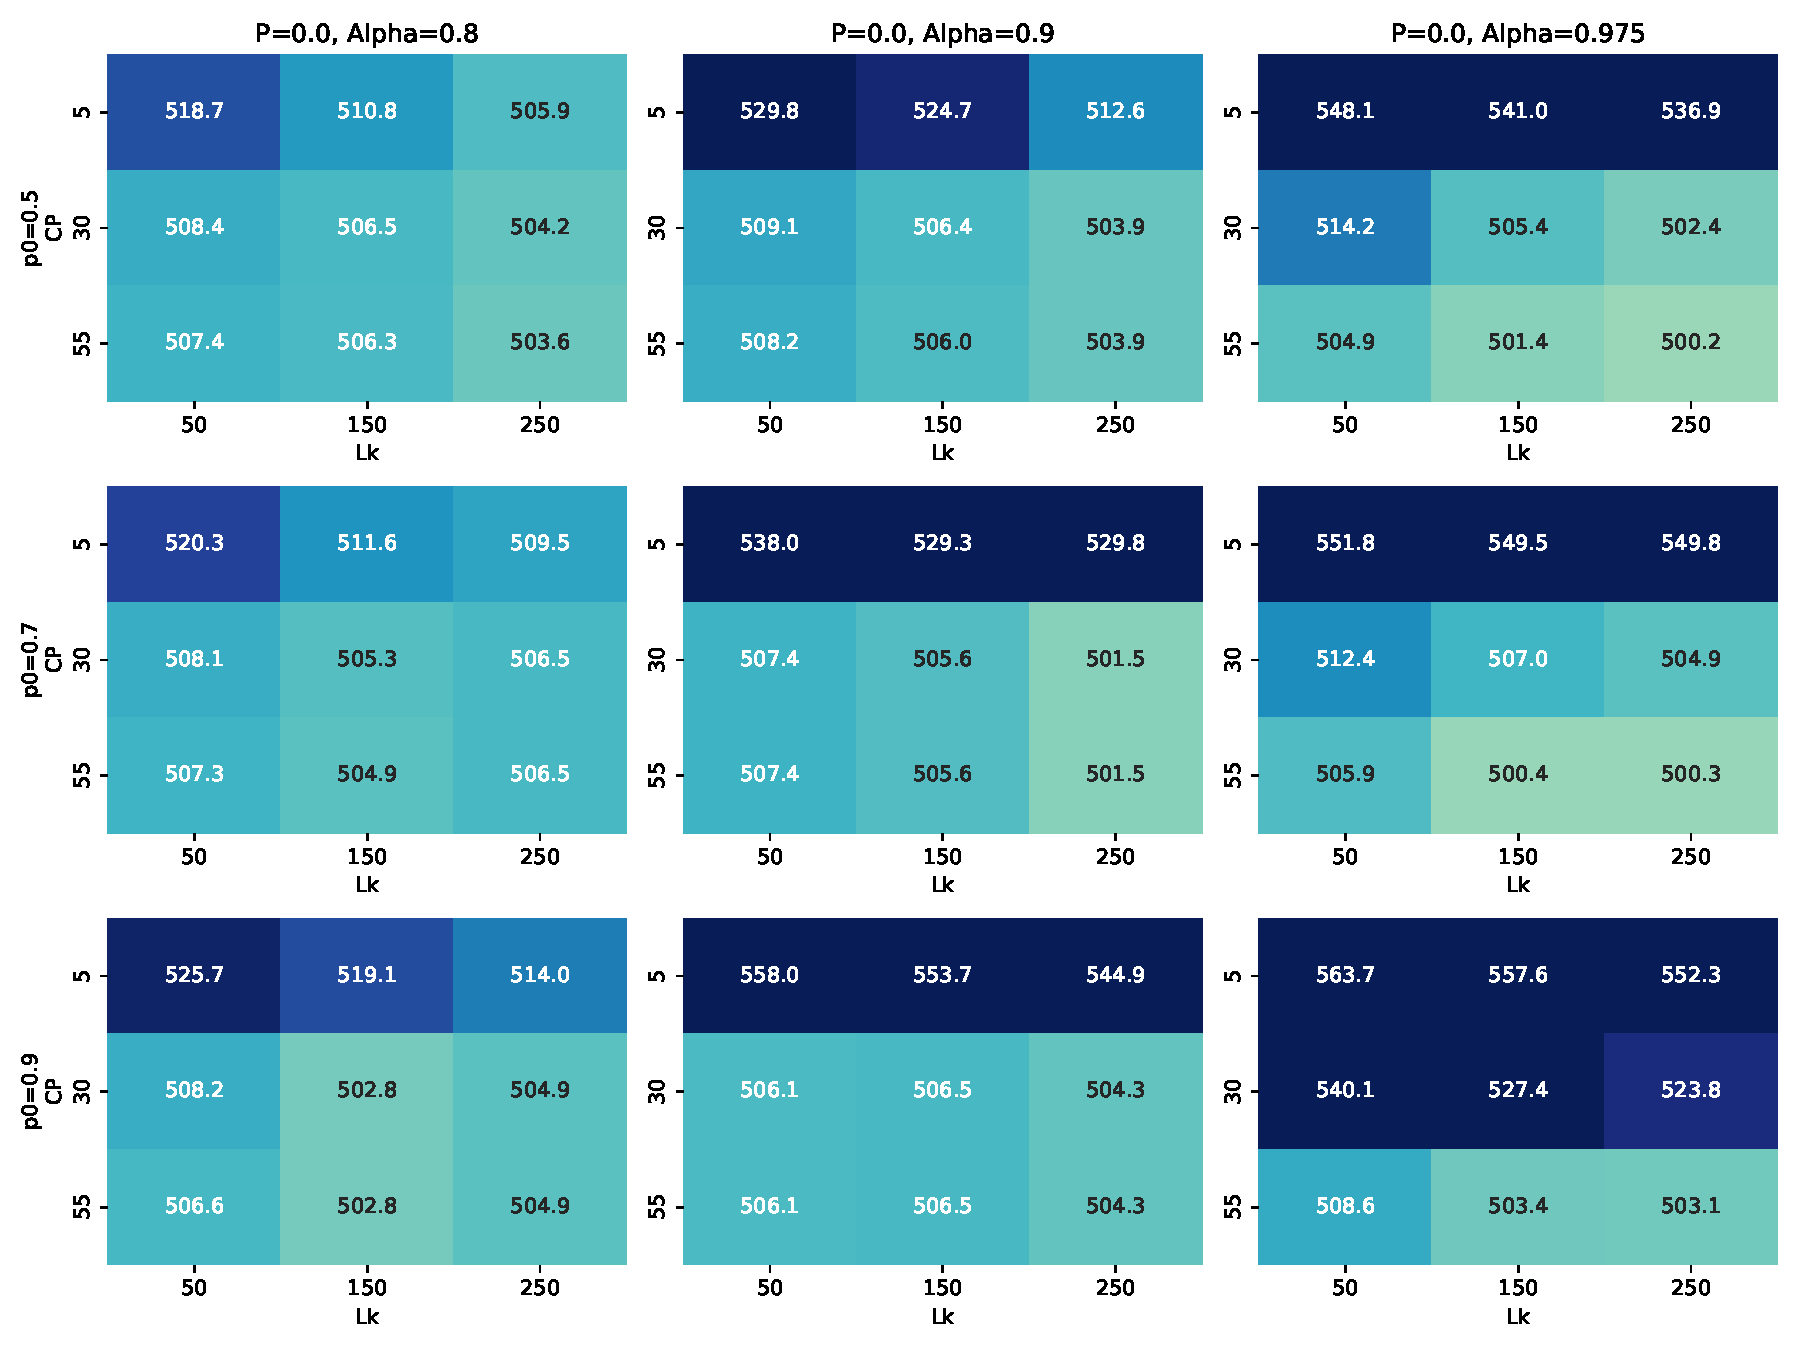
\includegraphics[width = \textwidth]{P1M2_GV_END_objf}
		\caption{Média do mínimo de \textit{makespan}}
		\label{fig:P1M2_GV_END_objf}
	\end{subfigure}
	\begin{subfigure}{0.49\textwidth}
	\centering
		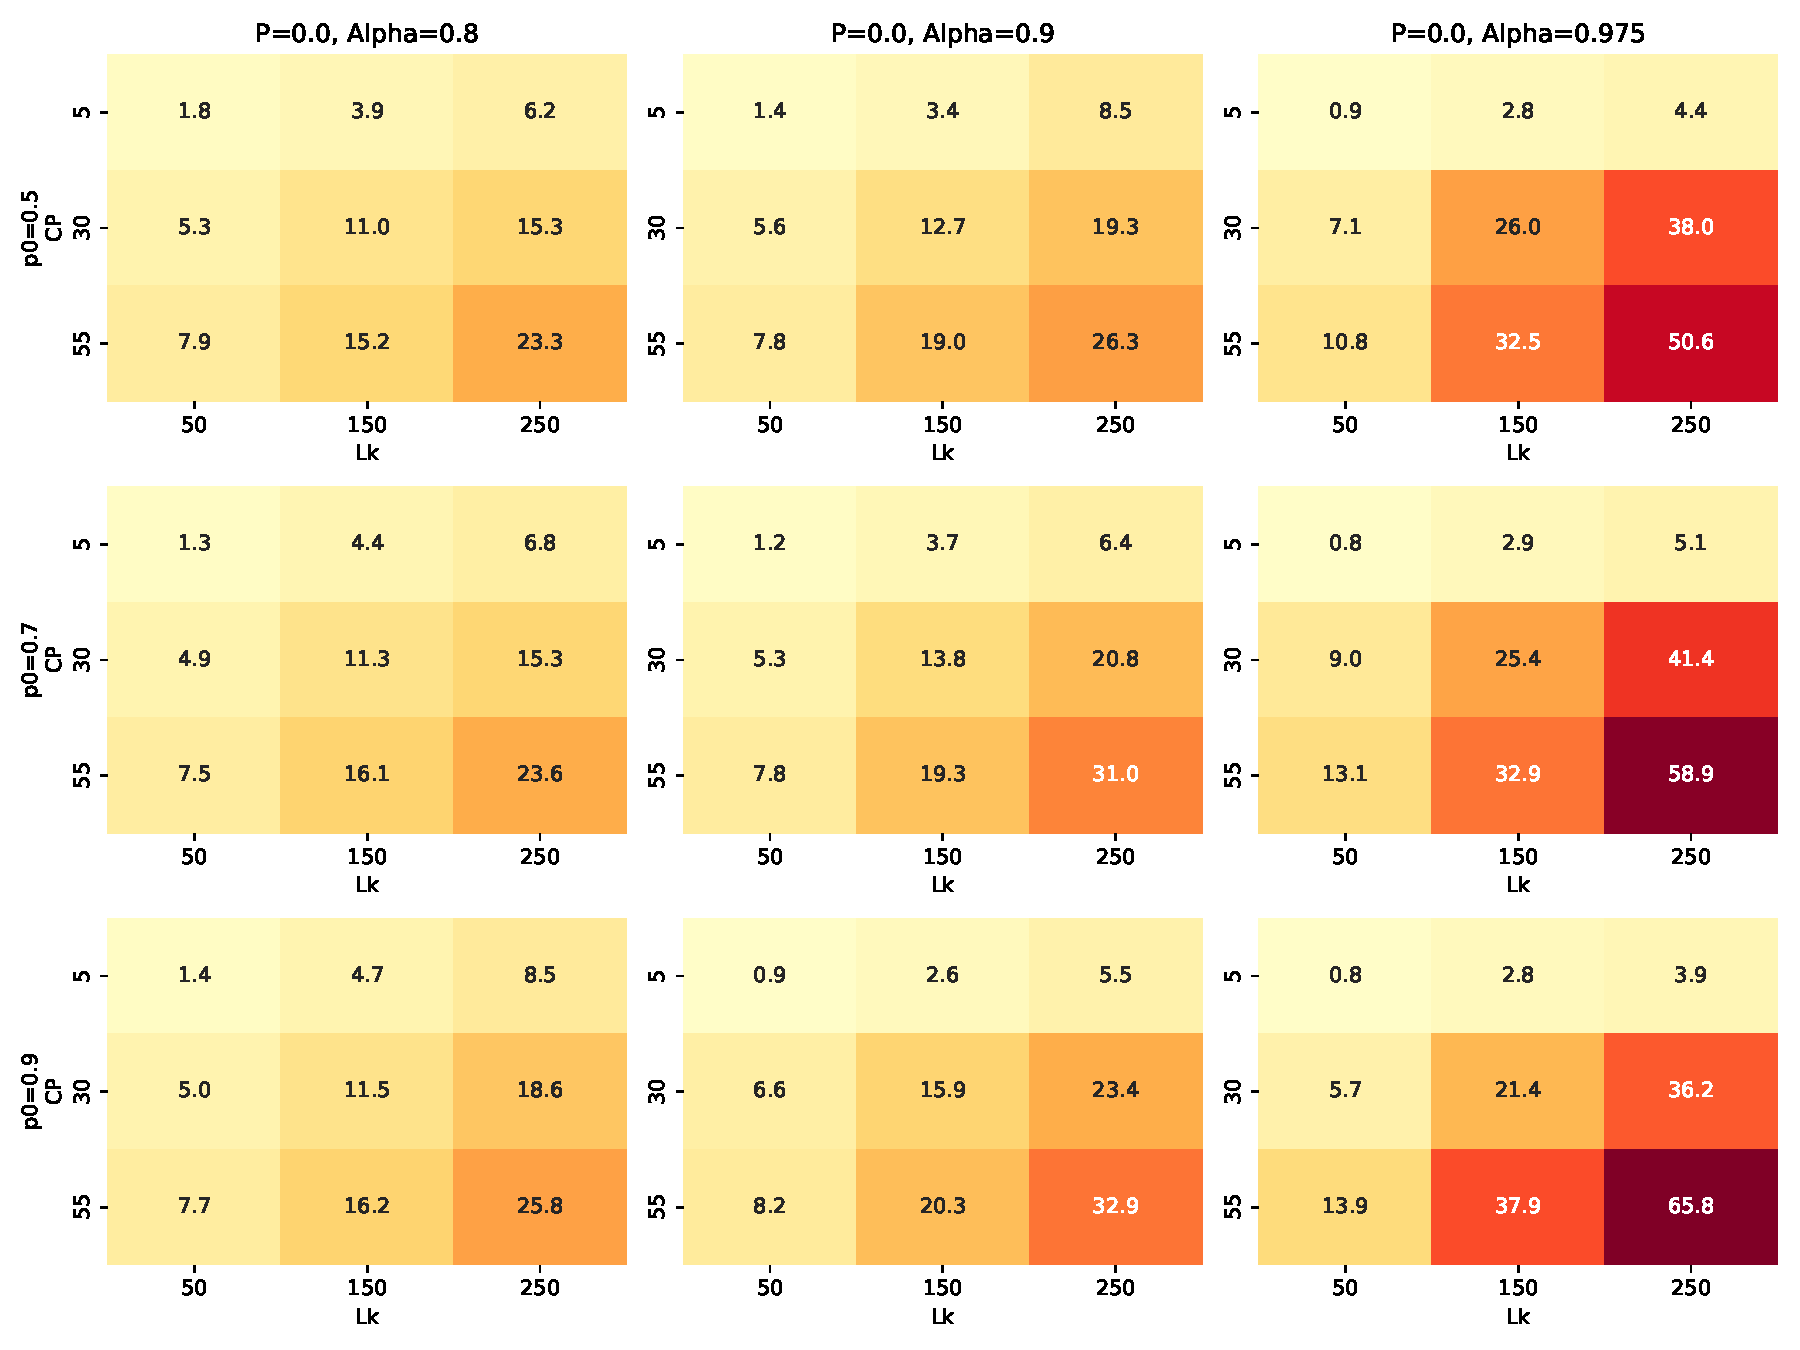
\includegraphics[width = \textwidth]{P1M2_GV_END_time}
		\caption{Média do máximo do tempo de computação}
		\label{fig:P1M2_GV_END_time}
	\end{subfigure}
	\label{fig:P1M2_GV_ND_alt}
	\centering
	\begin{subfigure}{0.49\textwidth}
	\centering
		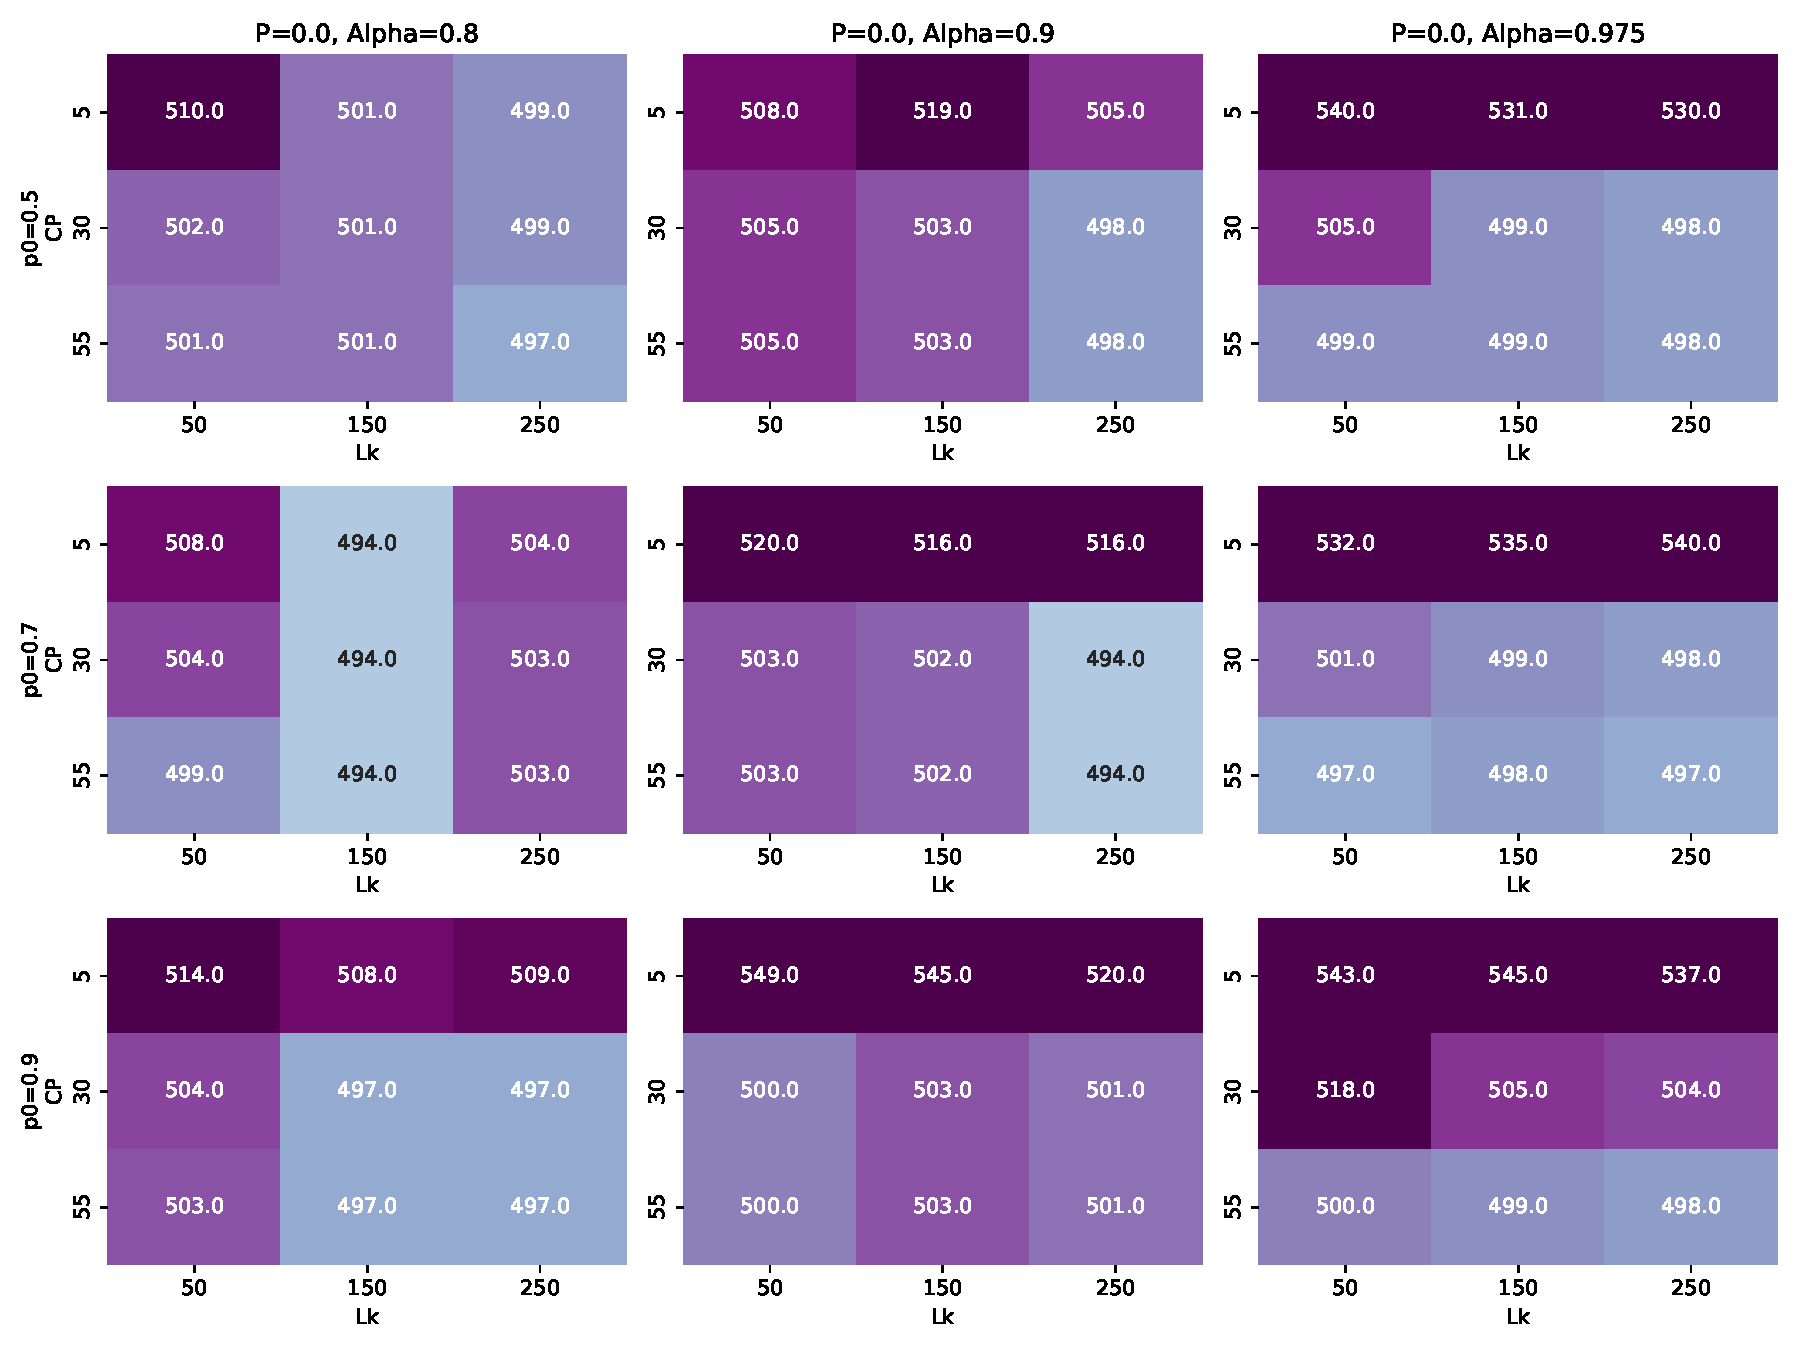
\includegraphics[width = \textwidth]{P1M2_GV_END_best}
		\caption{Melhor \textit{makespan}}
		\label{fig:P1M2_GV_END_best}
	\end{subfigure}
	\begin{subfigure}{0.49\textwidth}
	\centering
		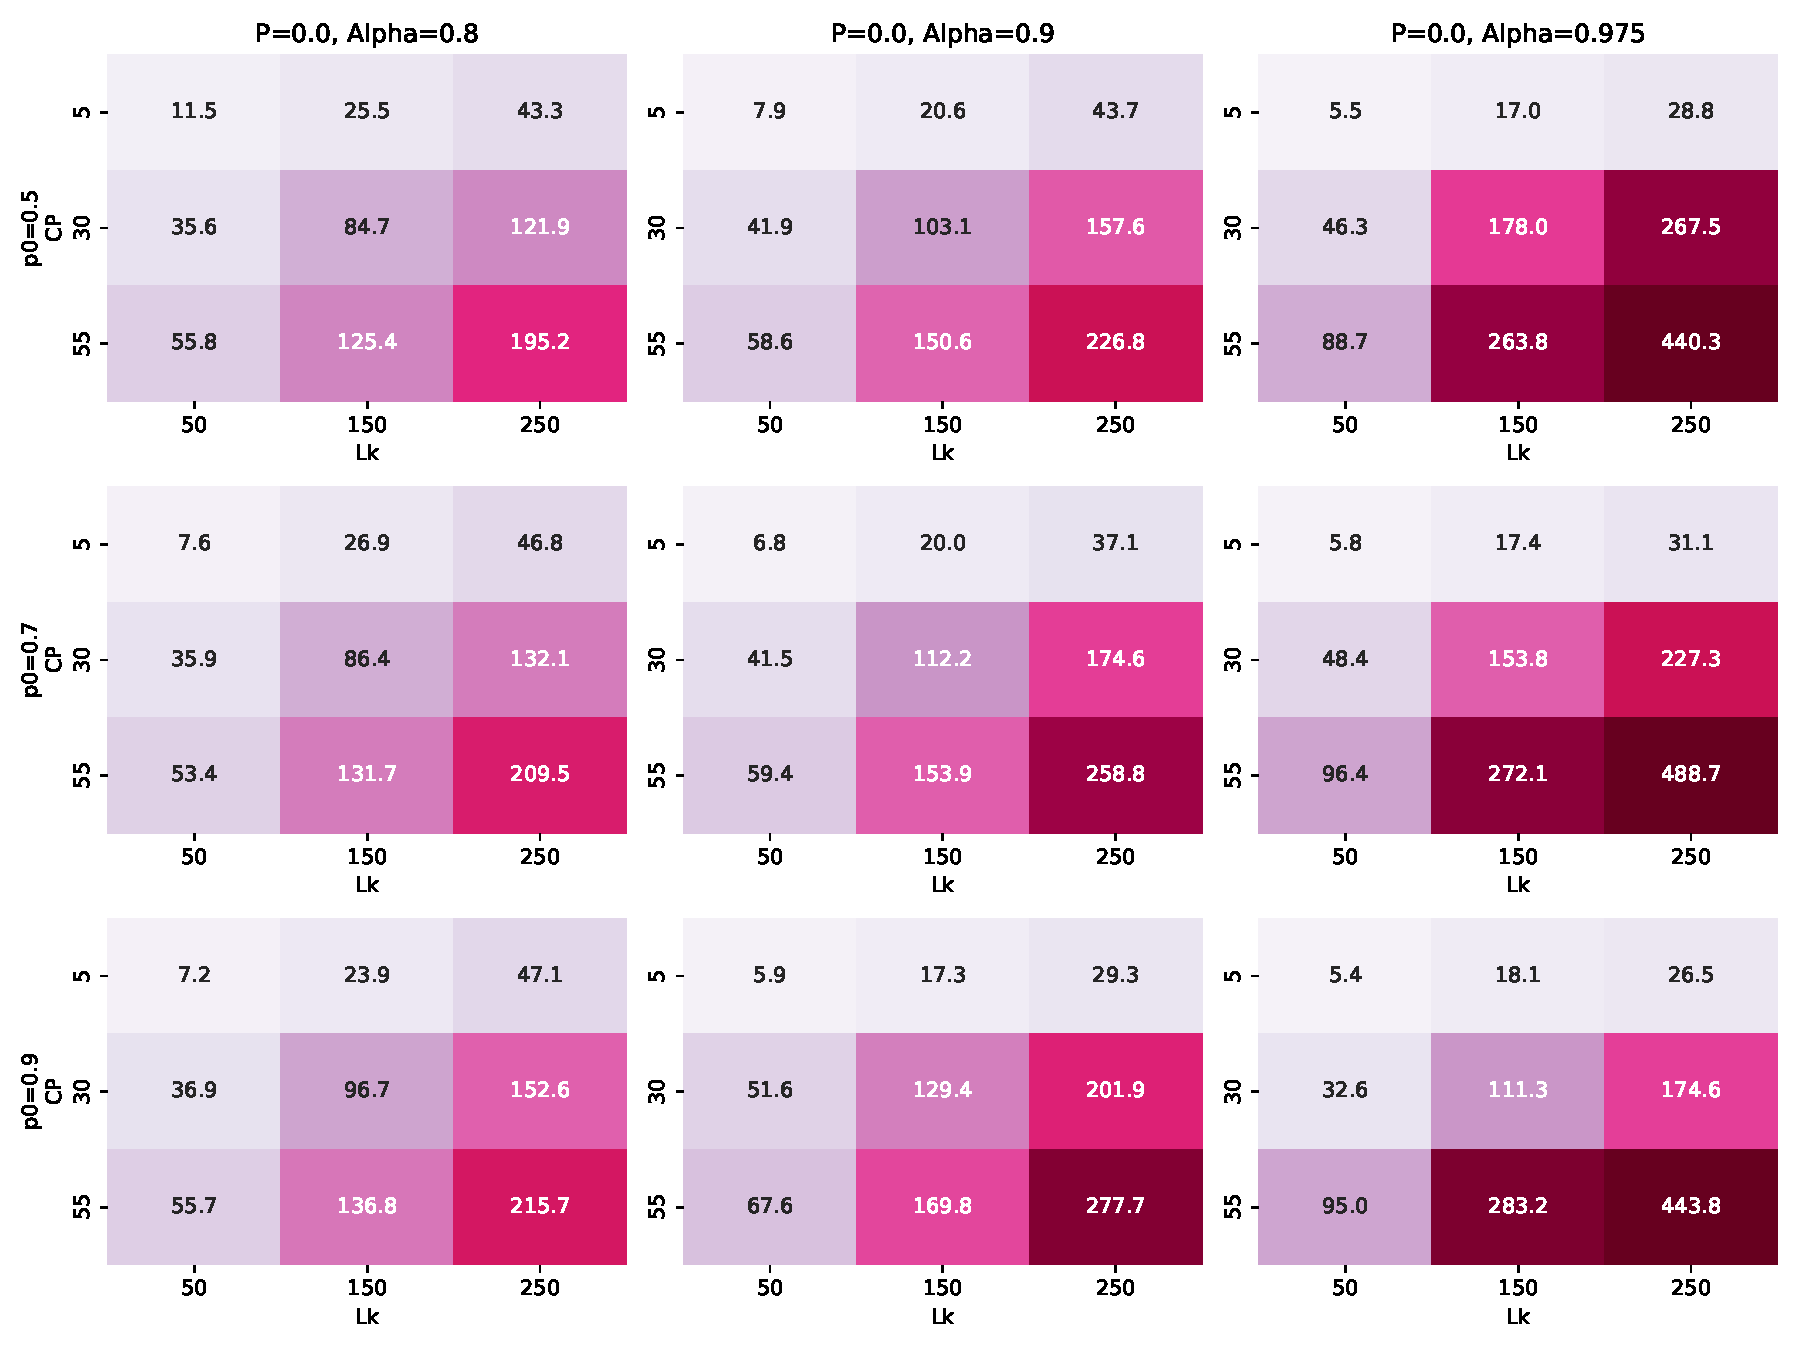
\includegraphics[width = \textwidth]{P1M2_GV_END_runtime}
		\caption{Tempo de computação total}
		\label{fig:P1M2_GV_END_runtime}
	\end{subfigure}
	\caption{Impacto dos níveis das variáveis sobre o valor da função objetivo e do tempo computacional para o Modelo 3 com \textit{enhanced non-delay} do problema de \textit{makespan}.}
	\label{fig:P1M2_GV_END_alt}
\end{figure}






\section{Problema do número de trabalhos}

\begin{figure}[H]
	\centering
	\begin{subfigure}{0.49\textwidth}
	\centering
		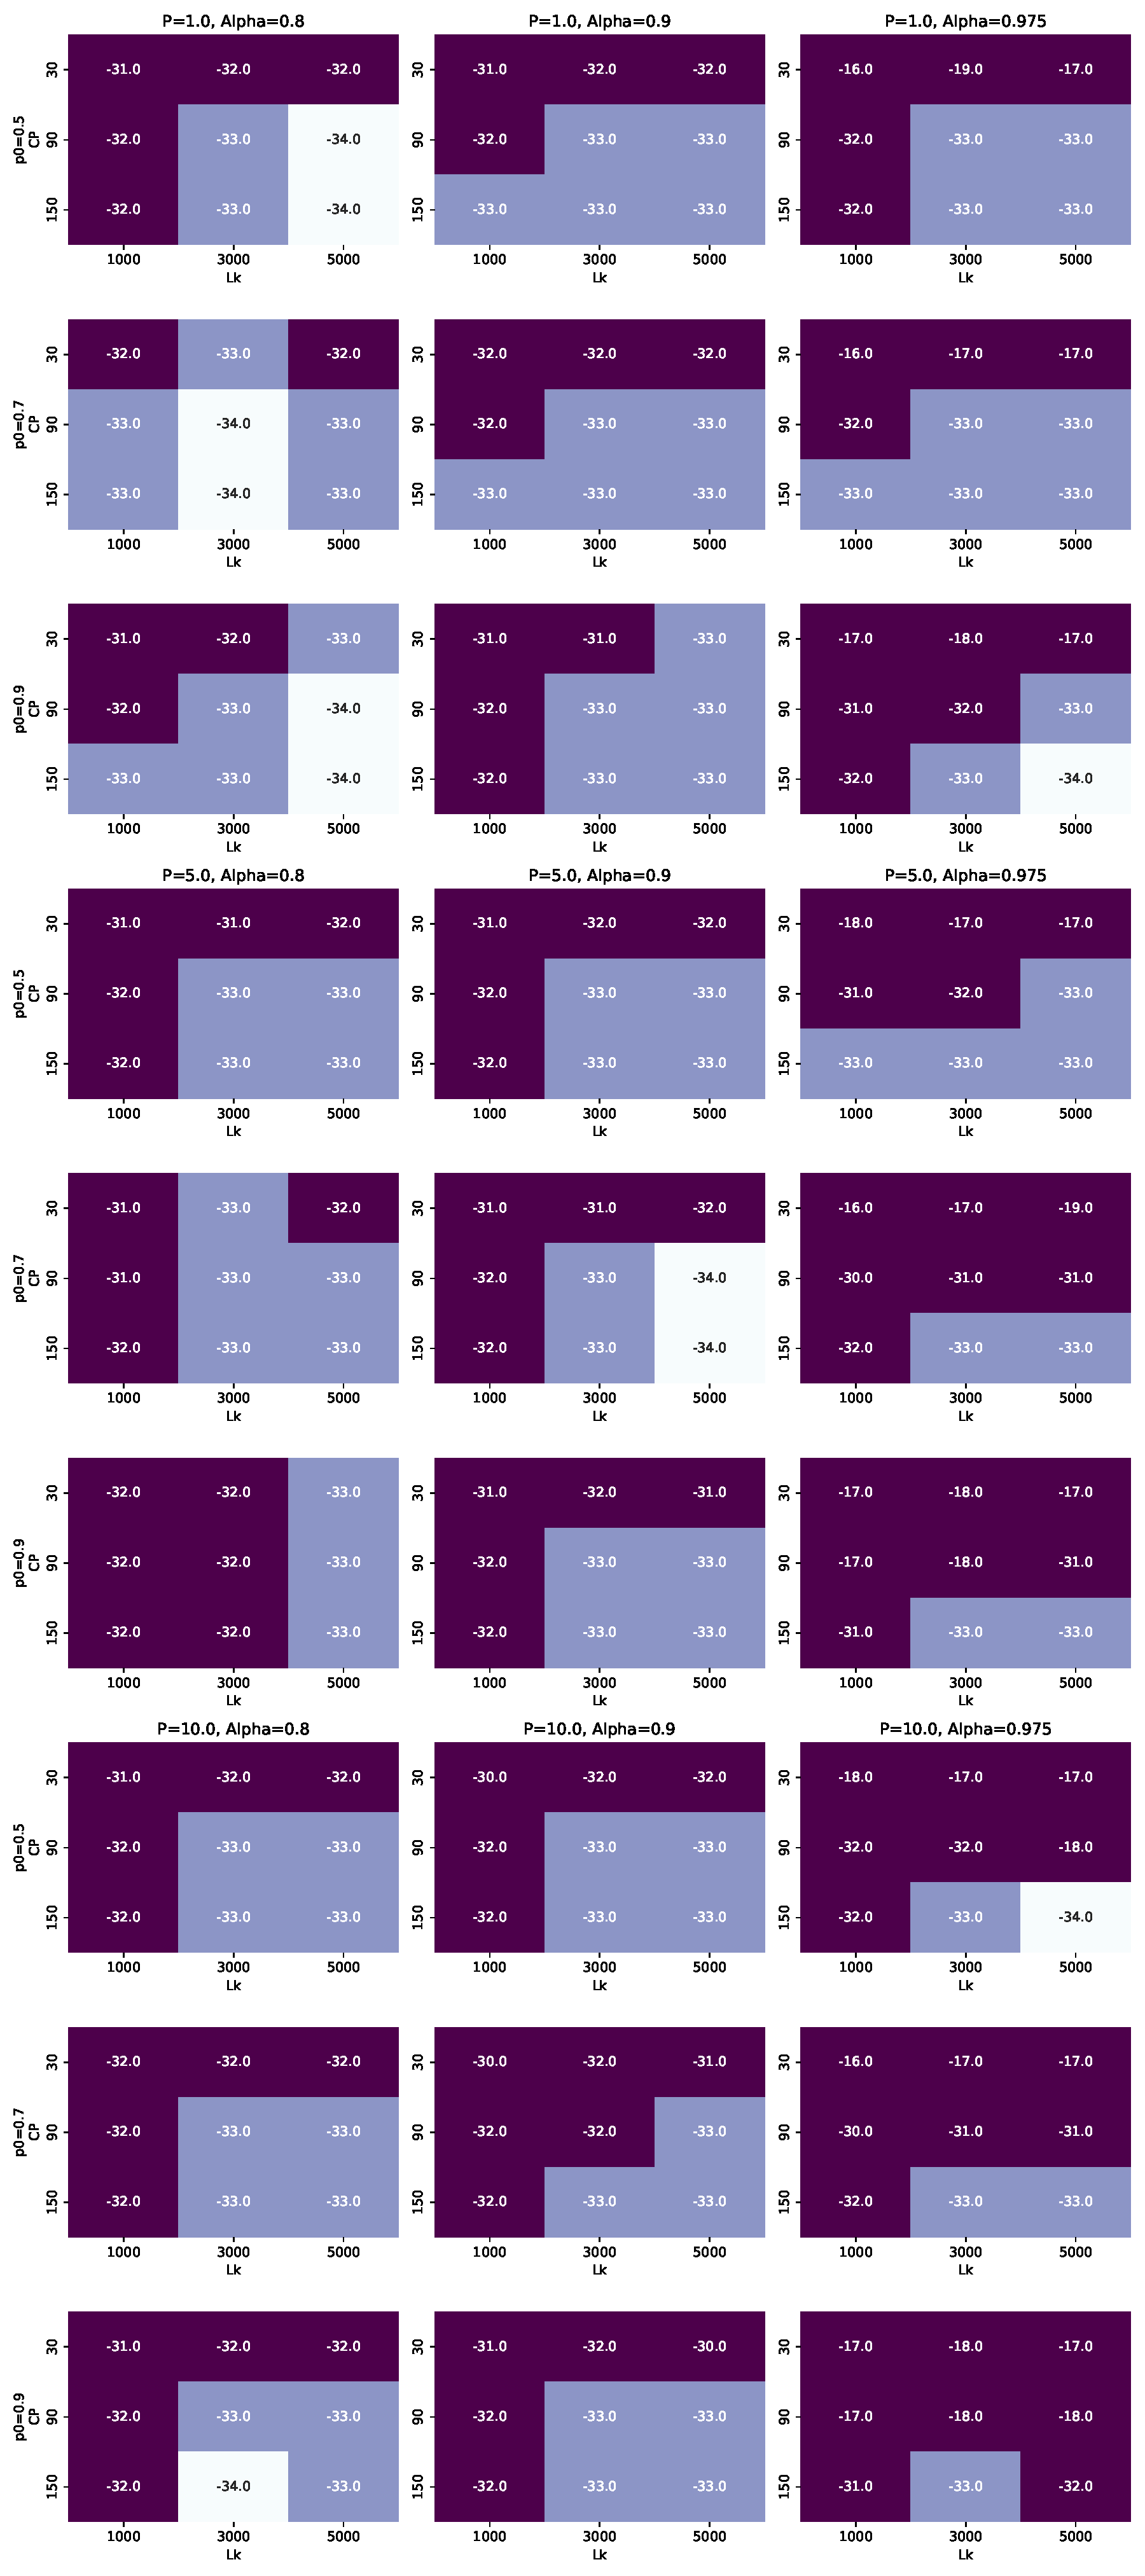
\includegraphics[width = \textwidth]{P2M1_NNGV_best}
		\caption{Melhor número de trabalhos}
		\label{fig:P2M1_NNGV_best}
	\end{subfigure}
	\begin{subfigure}{0.49\textwidth}
	\centering
		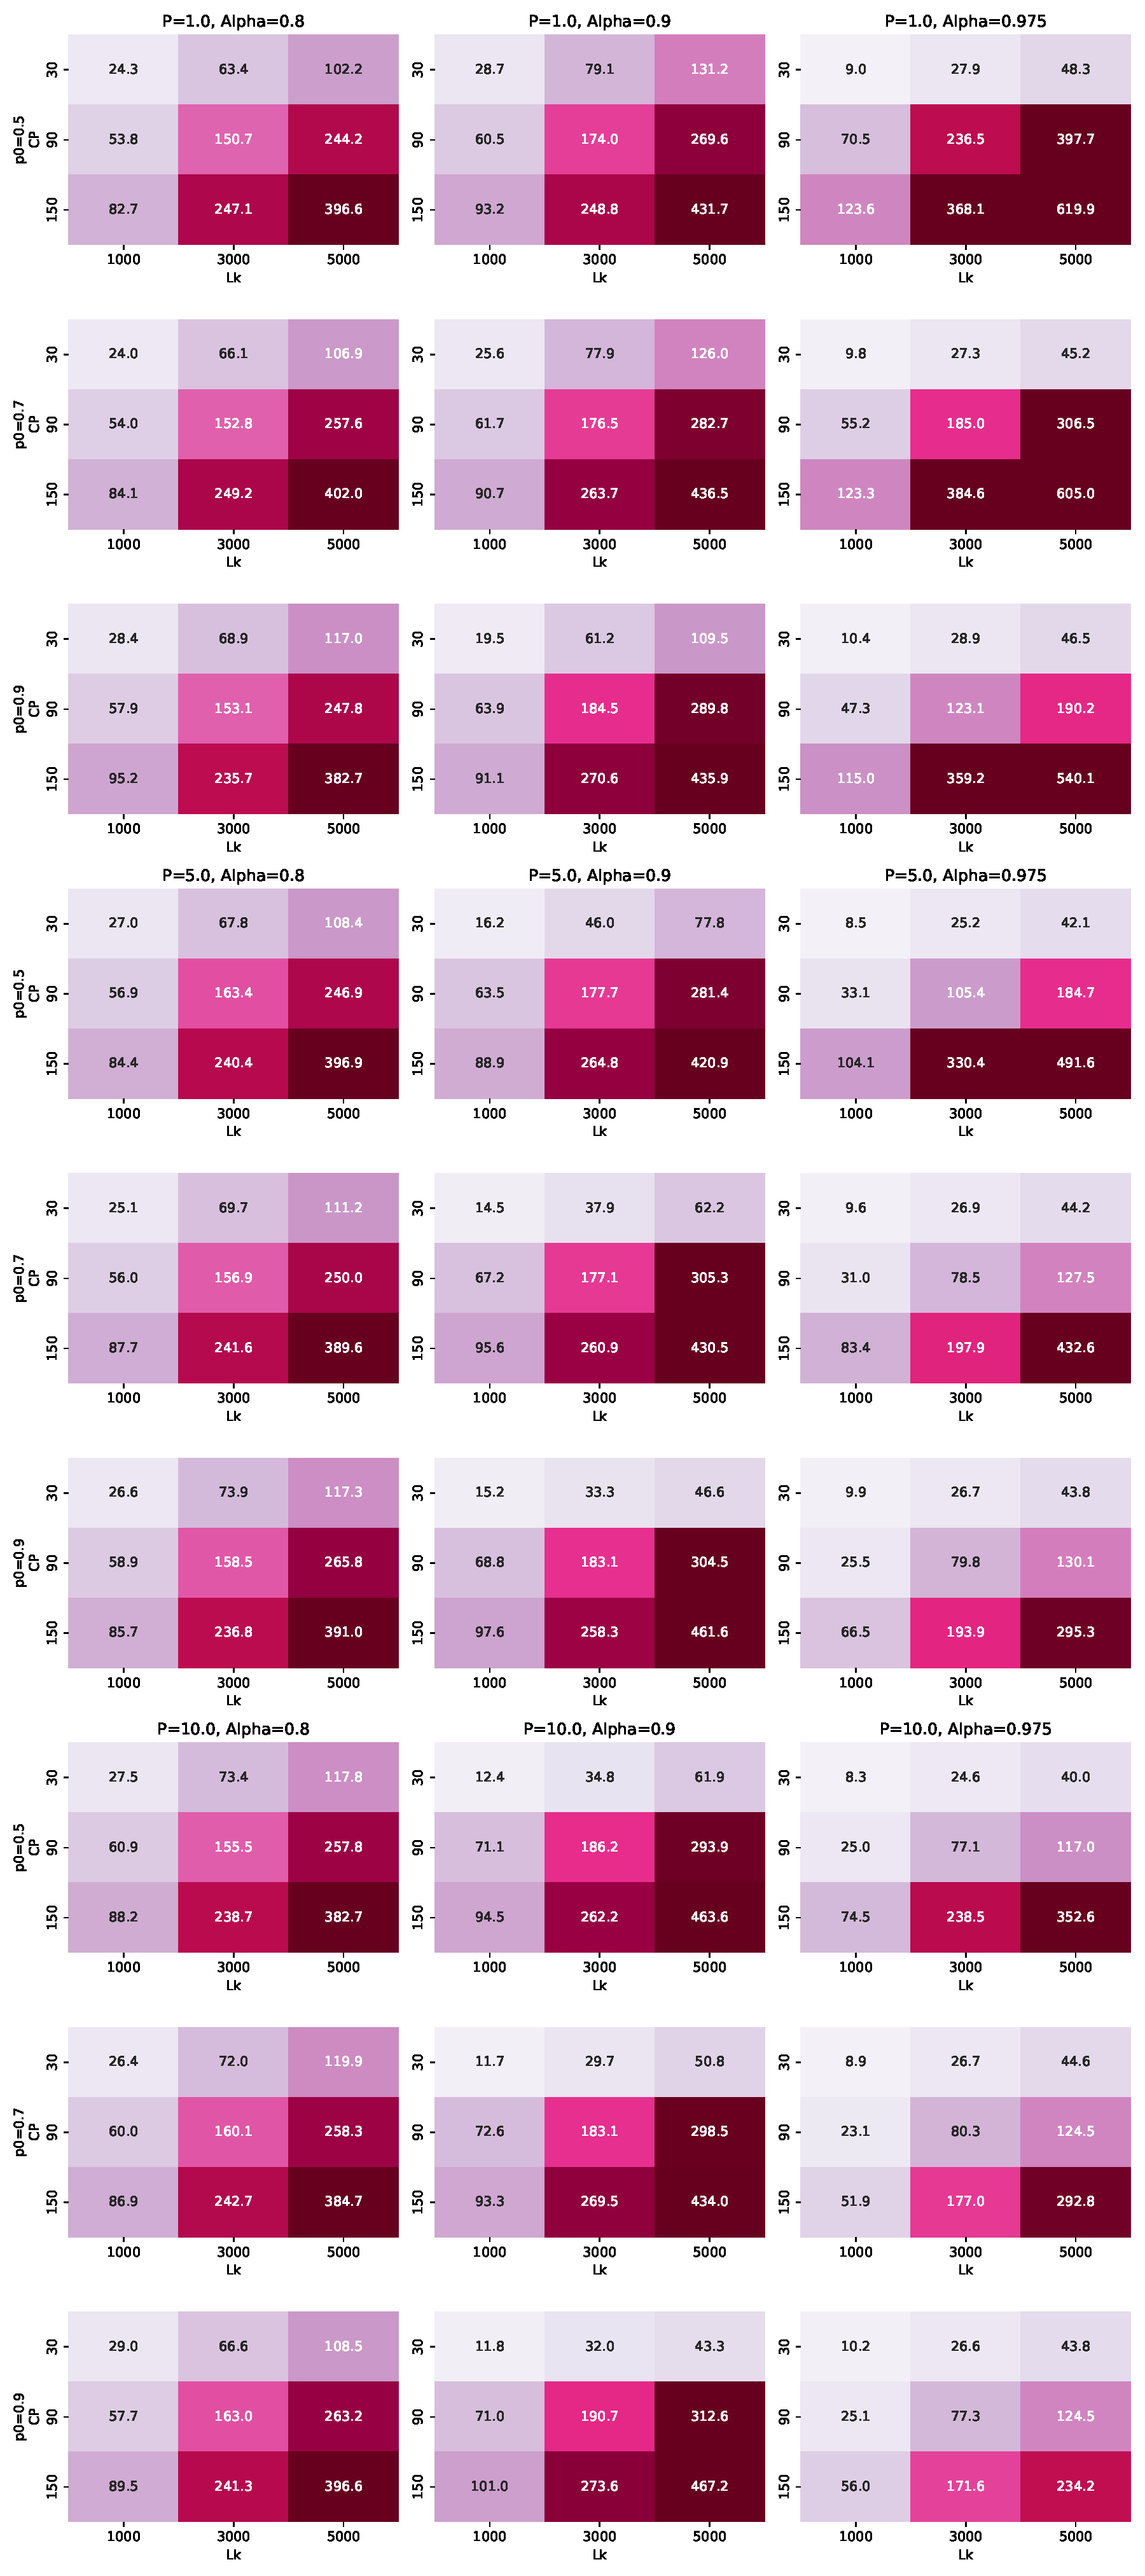
\includegraphics[width = \textwidth]{P2M1_NNGV_runtime}
		\caption{Tempo de computação total}
		\label{fig:P2M1_NNGV_runtime}
	\end{subfigure}
	\caption{Impacto dos níveis das variáveis sobre o valor da função objetivo e do tempo computacional para o Modelo 1 do problema do número de trabalhos.}
	\label{fig:P2M1_NNGV_alt}
\end{figure}

\begin{figure}[H]
	\centering
	\begin{subfigure}{0.49\textwidth}
	\centering
		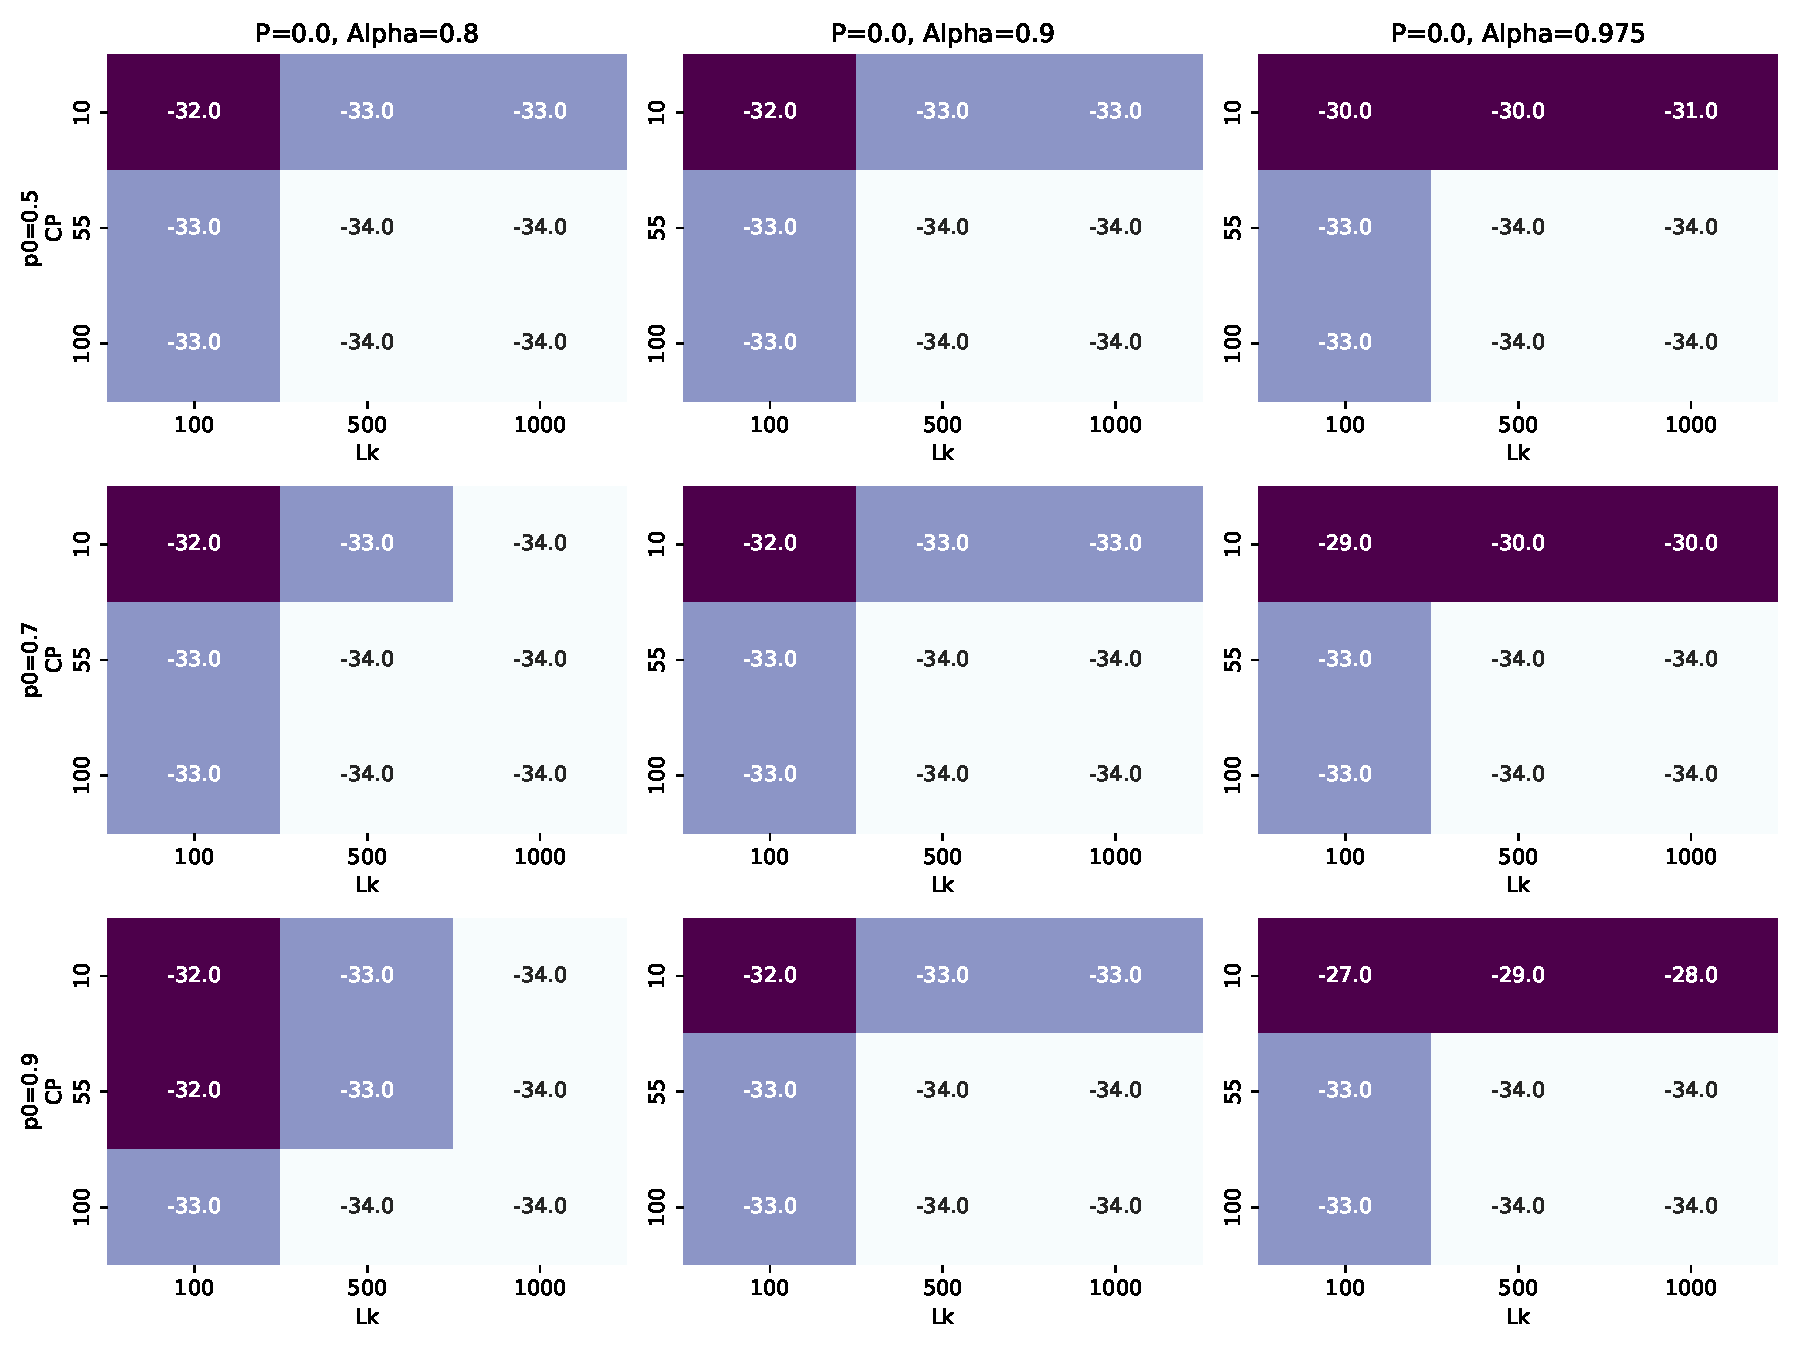
\includegraphics[width = \textwidth]{P2M1_GV_best}
		\caption{Melhor número de trabalhos}
		\label{fig:P2M1_GV_best}
	\end{subfigure}
	\begin{subfigure}{0.49\textwidth}
	\centering
		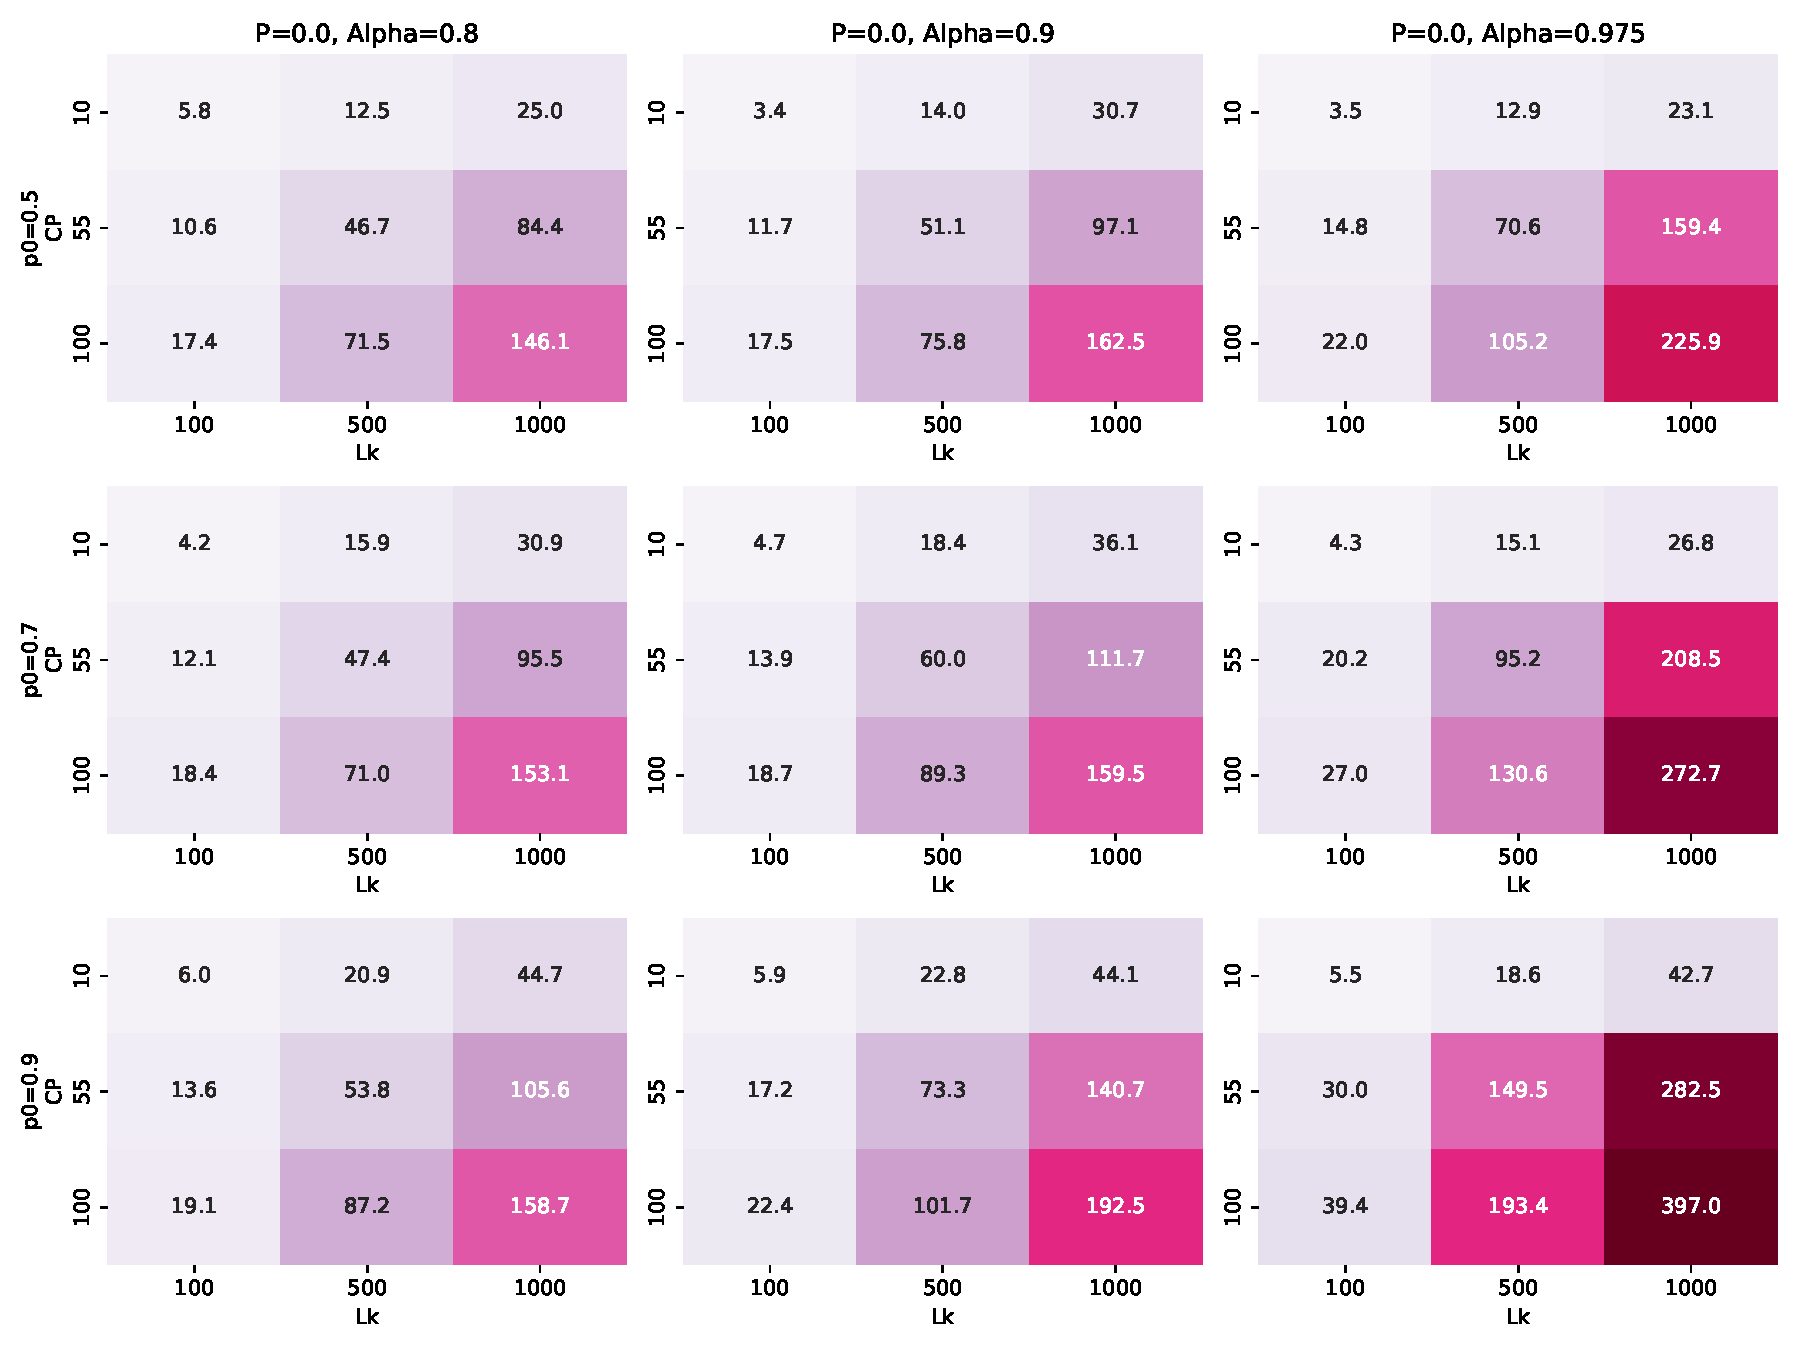
\includegraphics[width = \textwidth]{P2M1_GV_runtime}
		\caption{Tempo de computação total}
		\label{fig:P2M1_GV_runtime}
	\end{subfigure}
	\caption{Impacto dos níveis das variáveis sobre o valor da função objetivo e do tempo computacional para o Modelo 2 do problema do número de trabalhos.}
	\label{fig:P2M1_GV_alt}
\end{figure}

\begin{figure}[H]
	\centering
	\begin{subfigure}{0.49\textwidth}
	\centering
		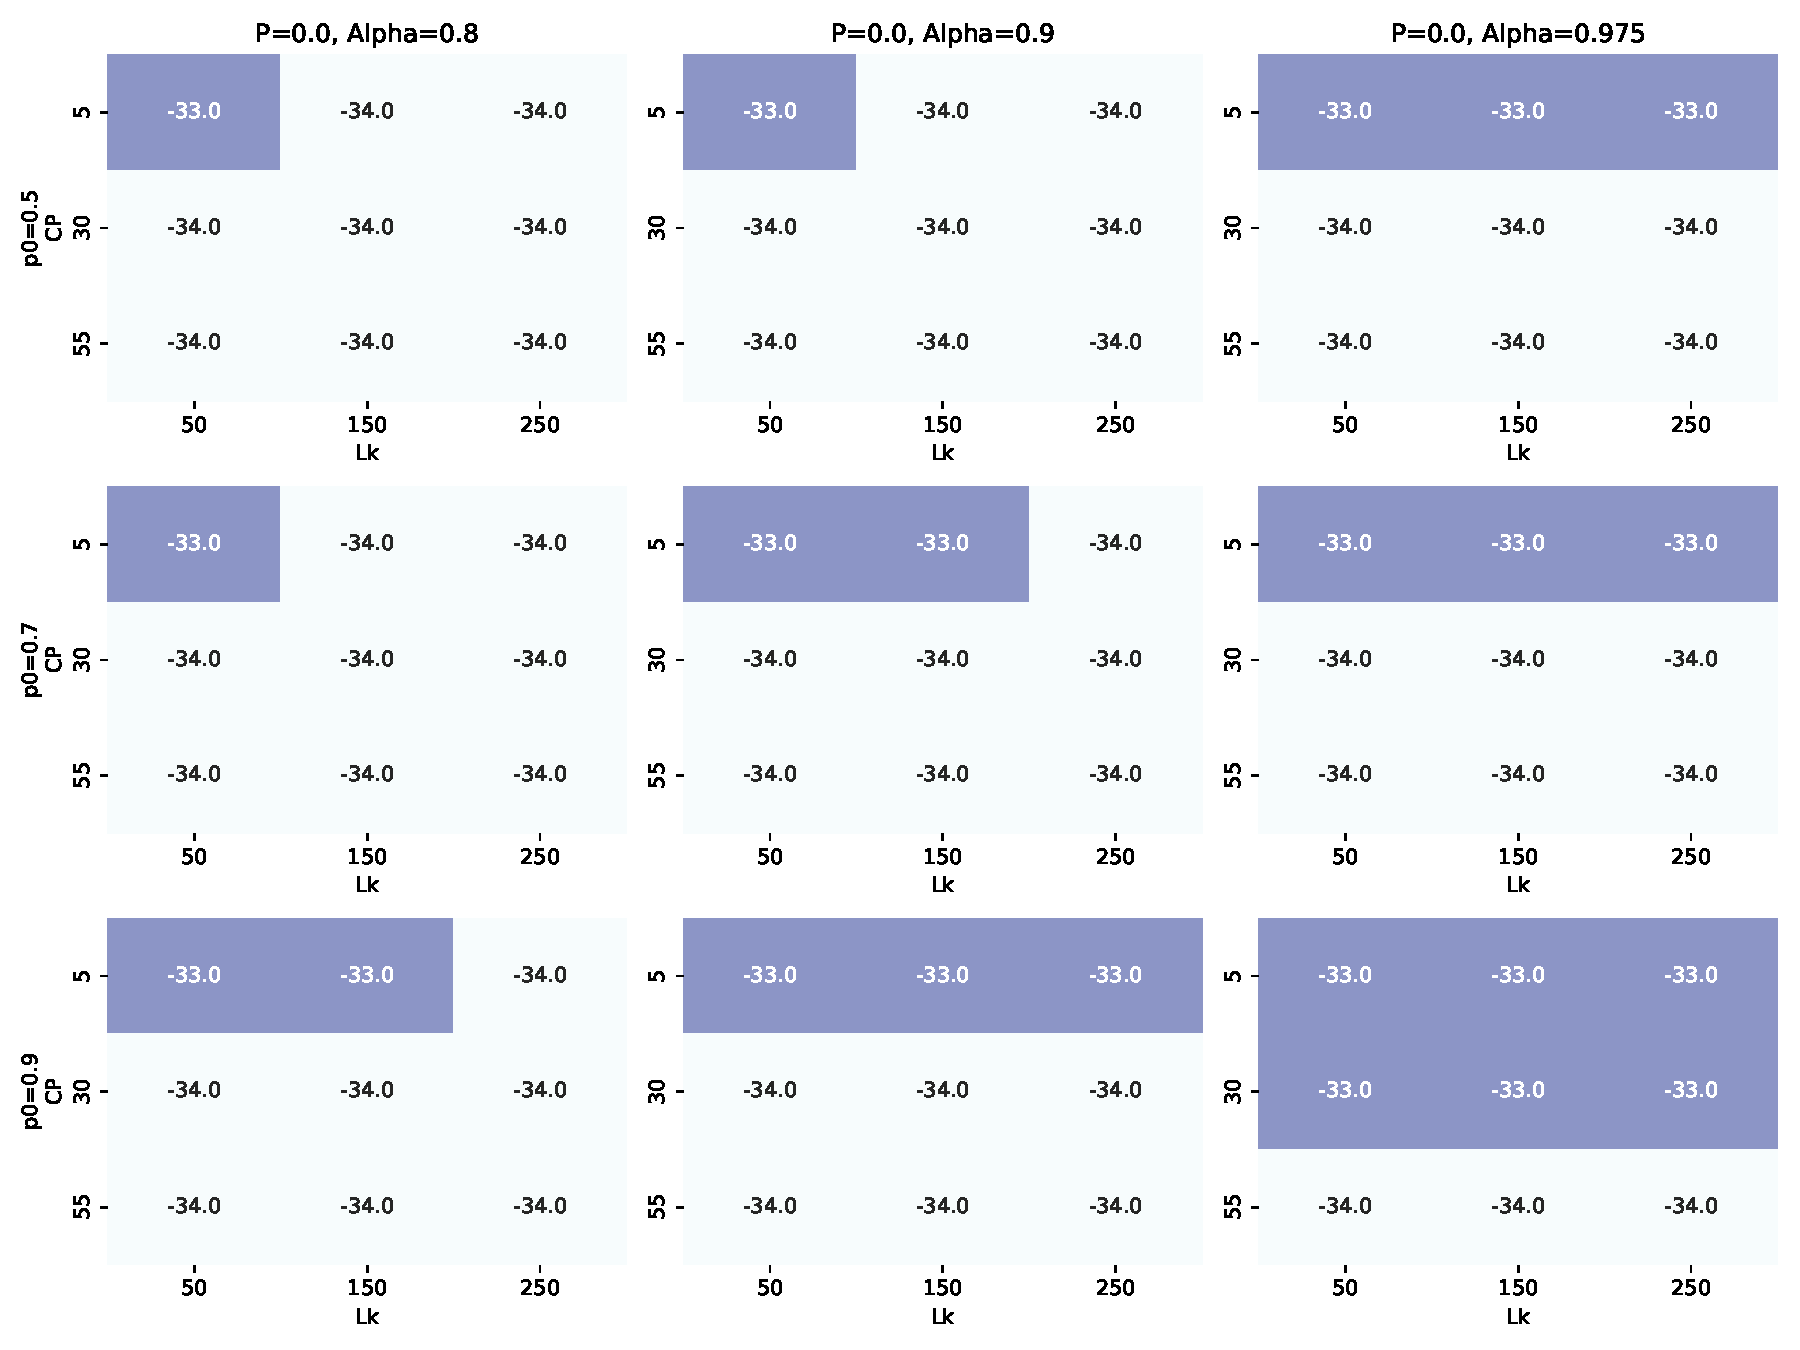
\includegraphics[width = \textwidth]{P2M2_GV_alt_best}
		\caption{Melhor número de trabalhos}
		\label{fig:P2M2_GV_alt_best}
	\end{subfigure}
	\begin{subfigure}{0.49\textwidth}
	\centering
		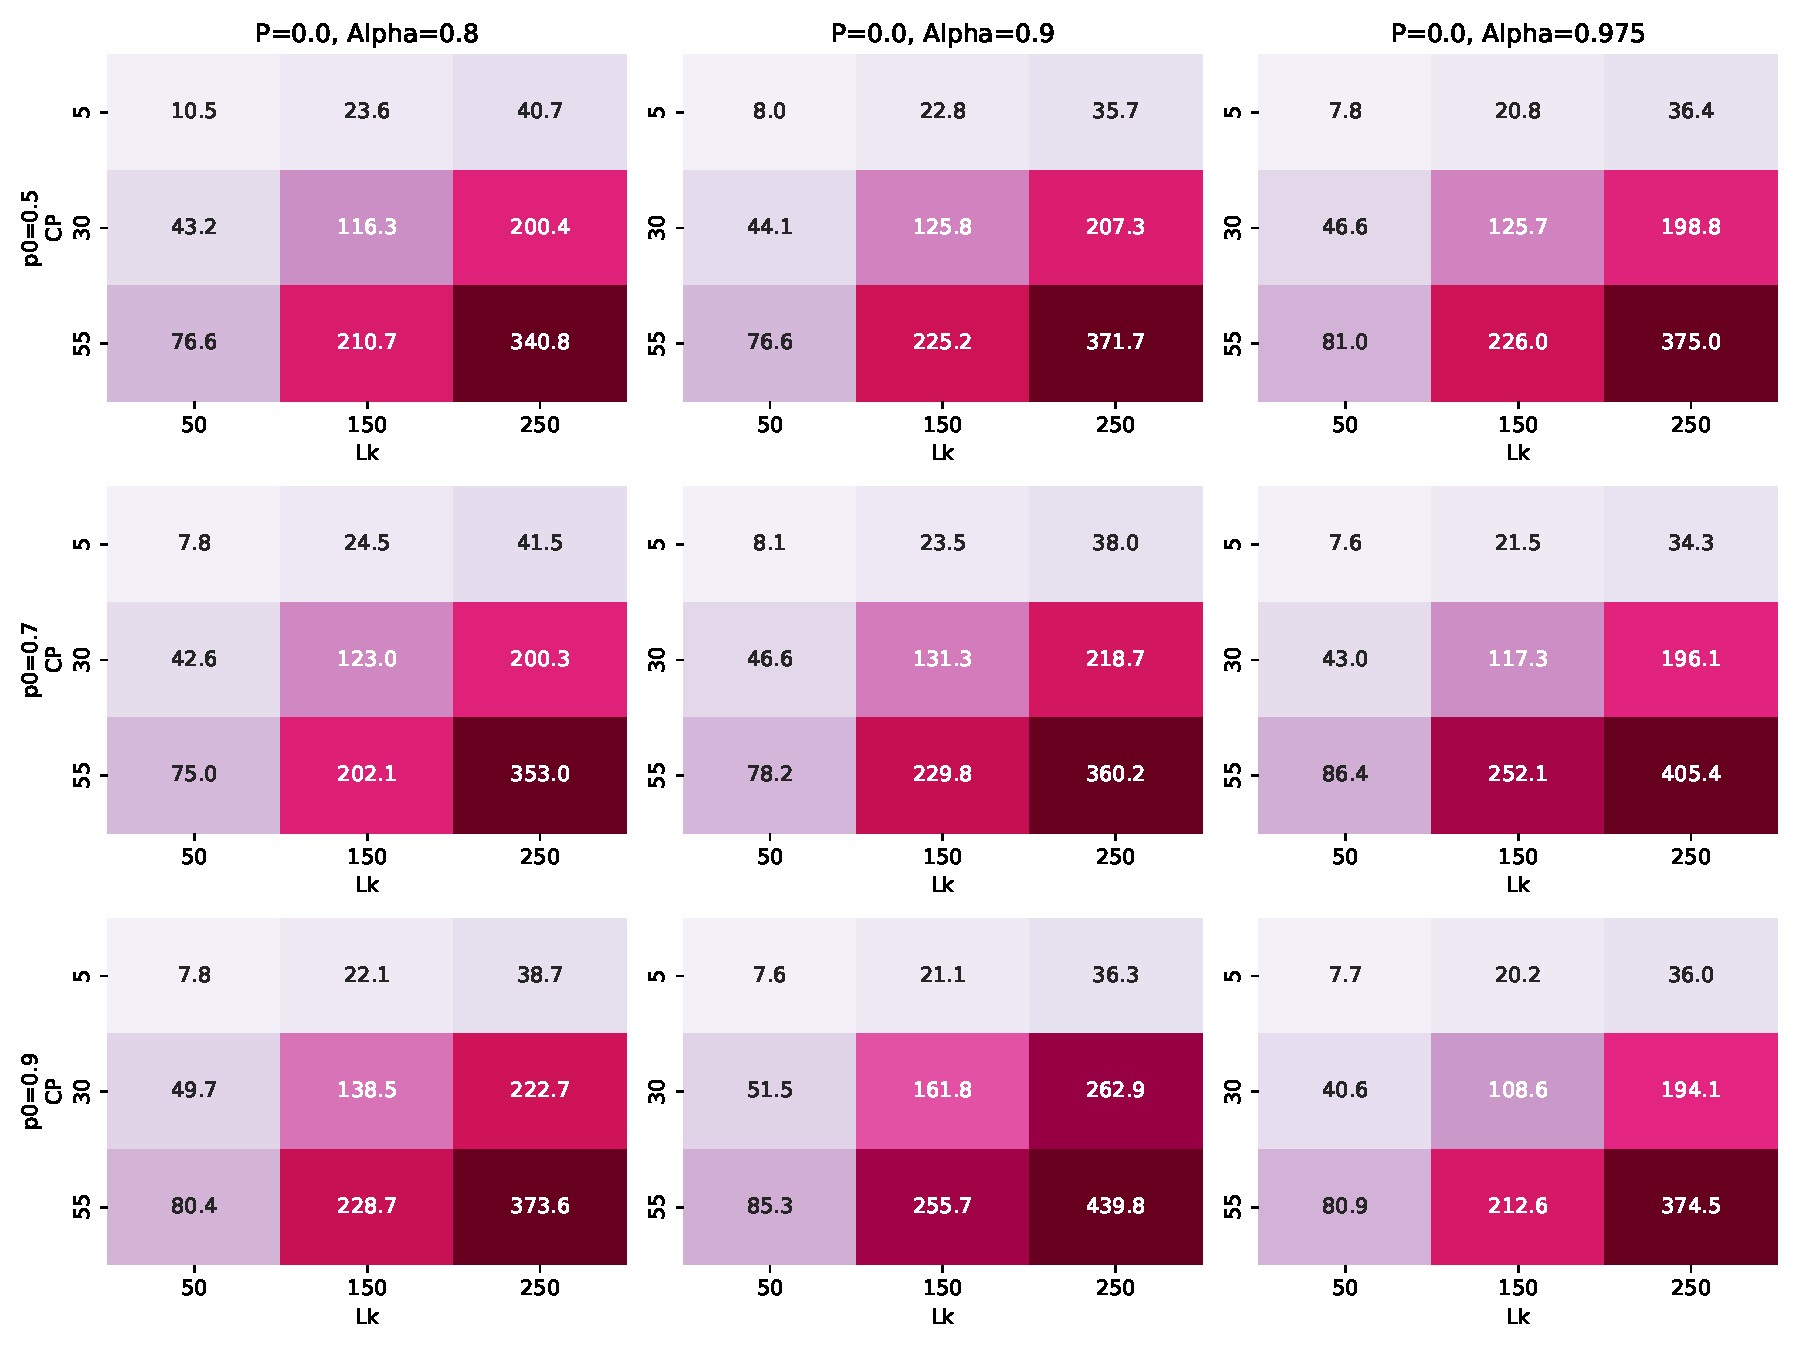
\includegraphics[width = \textwidth]{P2M2_GV_alt_runtime}
		\caption{Tempo de computação total}
		\label{fig:P2M2_GV_alt_runtime}
	\end{subfigure}
	\caption{Impacto dos níveis das variáveis sobre o valor da função objetivo e do tempo computacional para o Modelo 3 do problema do número de trabalhos.}
	\label{fig:P2M2_GV_alt_alt}
\end{figure}


\chapter{Algoritmos}
\label{chp:algo}

\section{Problema de \textit{Makespan}}

\newpage

\begin{algorithm}[H]
\label{algo:P1M1_main_algo}
	$i \gets$ U(0,$n$)\;
    $q \gets$ U(0,1)\;
    $d \gets$ duração[i]\;
    $\delta \gets$ tipo\_exame\_delta[i]\;
    $t_{velho} \gets S_{[i]}$\;
    \tcp{Retirar da matriz de utilização de recursos $u$, a utilização relativa a $i$}
    $u_{[t_{velho}: t_{velho}+d]} \gets u_{[t_{velho}: t_{velho}+d]} - \delta$\;
    \tcp{\textit{ini} e \textit{fim} provenientes da iteração anterior}
    $t_{novo} \gets \text{U(ini, fim-d)}$\;
    \tcp{Modificar a matriz $S$ no índice $i$ de forma a começar no novo instante $t_{novo}$}
    $S_{[i]} \gets t_{novo}$\;
    \tcp{Adicionar à matriz de utilização de recursos $u$, a utilização relativa a $i$}
    $u_{[t_{novo}: t_{novo}+d]} \gets u_{[t_{novo}: t_{novo}+d]} + \delta$\;
    \textit{ini} $\gets \min(S)$\;
    \textit{fim} $\gets \max(S+\text{duração})$\;
    $C_{\max} \gets \text{fim} - \text{ini}$\;
    $f(s') \gets C_{\max} + P \sum_{t=ini}^{fim-1}\sum_{p}v(t,p)$\;
    \If{$f(s')<f(s)$ ou $q < exp((f(s)-f(s'))/c)$}
	{
		$s \gets s'$\;
		\If{$f(s')<f(s^*)$}
		{
			$s^* \gets s'$
		}
	}
	\Else
	{
		$S_{[i]} \gets t_{velho}$\;
    	$u_{[t_{velho}: t_{velho}+d]} \gets u_{[t_{velho}: t_{velho}+d]} + \delta$\;
		$u_{[t_{novo}: t_{novo}+d]} \gets u_{[t_{novo}: t_{novo}+d]} - \delta$;\
	}    
    \caption{Pseudo-código de geração de novos vizinhos, a sua avaliação, aceitação ou rejeição, e retrocesso. Para o problema de \textit{makespan} com o Modelo 1.}
\end{algorithm}


\begin{algorithm}[H]
\label{algo:P1M1_cand_gen}
	$\text{Candidatos}=\{\}$\;
	\For{$t \gets \text{ini}$ \KwTo $\text{fim}-d$}
	{
		$u_{[t: t+d]} \gets u_{[t: t+d]} + \delta$\;
		\If{$u \leq C_{p}$}
		{	
			\tcp{Adicionar $t$ à lista de candidatos}
			$\text{Candidatos} \gets \text{Candidatos} \cup \{t\}$\;
		}
	}
	$\text{Candidatos} \gets \text{Candidatos} \cup \{\max(\text{ini}-d, 0)\}$\;
	$\text{Candidatos} \gets \text{Candidatos} \cup \{\min(\text{fim}+1, T_{max}-d)\}$\;
	\Return Candidatos
    \caption{Pseudo-código que gera os instantes candidatos durante a criação da vizinhança.}
    \label{algo:cand}
\end{algorithm}

\begin{algorithm}[H]
\label{algo:P1M1_GV_main_algo}
	$i \gets$ U(0,$n$)\;
    $q \gets$ U(0,1)\;
    $d \gets$ duração[i]\;
    $\delta \gets$ tipo\_exame\_delta[i]\;
    $t_{velho} \gets S_{[i]}$\;
    \tcp{Retirar da matriz de utilização de recursos $u$, a utilização relativa a $i$}
    $u_{[t_{velho}: t_{velho}+d]} \gets u_{[t_{velho}: t_{velho}+d]} - \delta$\;
    $t_{novo} \gets \text{Candidatos}[\text{U(0, |Candidatos}|-1)]$\;
    \tcp{Modificar a matriz $S$ no índice $i$ de forma a começar no novo instante $t_{novo}$}
    $S_{[i]} \gets t_{novo}$\;
    \tcp{Adicionar à matriz de utilização de recursos $u$, a utilização relativa a $i$}
    $u_{[t_{novo}: t_{novo}+d]} \gets u_{[t_{novo}: t_{novo}+d]} + \delta$\;
    \textit{ini} $\gets \min(S)$\;
    \textit{fim} $\gets \max(S+\text{duração})$\;
    $C_{\max} \gets \text{fim} - \text{ini}$\;
    $f(s') \gets C_{\max}$\;
    \If{$f(s')<f(s)$ ou $q < exp((f(s)-f(s'))/c)$}
	{
		$s \gets s'$\;
		\If{$f(s')<f(s^*)$}
		{
			$s^* \gets s'$
		}
	}
	\Else
	{
		$S_{[i]} \gets t_{velho}$\;
    	$u_{[t_{velho}: t_{velho}+d]} \gets u_{[t_{velho}: t_{velho}+d]} + \delta$\;
		$u_{[t_{novo}: t_{novo}+d]} \gets u_{[t_{novo}: t_{novo}+d]} - \delta$;\
	}    
    \caption{Pseudo-código de geração de novos vizinhos, a sua avaliação, aceitação ou rejeição, e retrocesso. Para o problema de \textit{makespan} com o Modelo 2.}
\end{algorithm}


\begin{algorithm}[H]
	\For{$t \gets \text{ini}$ \KwTo $\text{fim}-d$}
	{
		$u_{[t: t+d]} \gets u_{[t: t+d]} + \delta$\;
		\If{$u \leq C_{p}$}
		{
			\Return t
		}
	}
	\Return -1
    \caption{Pseudo-código do algoritmo para encontrar o instante mais cedo possível.}
    \label{algo:earliest_t}
\end{algorithm}

\begin{algorithm}[H]
    $S^{\textit{forward}} \gets \{\}$\;
    \For{$i \in \text{Sequência}$}
    {
        $d \gets \text{duração}[i]$\;
        $\delta \gets \text{tipo\_exame\_delta}[i]$\;
        $t \gets \text{instante\_mais\_cedo(\textit{ini},\textit{fim})}$\;
        $S^{\textit{forward}} \gets S^{\textit{forward}} \cup \{t\}$\;
        $u_{[t: t+d]} \gets u_{[t: t+d]} + \delta$\;
    }
    \caption{Pseudo-código de \textit{left-shift timetabling}}
    \label{algo:left-shift-TT}
\end{algorithm}

\begin{algorithm}[H]
    $S^{\textit{forward}} \gets \{\}$\;
    \For{$i \in \text{Sequência}$}
    {
        $d \gets \text{duração}[i]$\;
        $\delta \gets \text{tipo\_exame\_delta}[i]$\;
        $t \gets \text{instante\_mais\_cedo(\textit{ini},\textit{fim})}$\;
        $S^{\textit{forward}} \gets S^{\textit{forward}} \cup \{t\}$\;
        $u_{[t: t+d]} \gets u_{[t: t+d]} + \delta$\;
    }
    $S^{\textit{backward}} \gets \{\}$\;
    Sequência $\gets$ Sequência.flip()\;
	\For{$i \in \text{Sequência}$}
	{
        $d \gets \text{duração}[i]$\;
        $\delta \gets \text{tipo\_exame\_delta}[i]$\;
        $\delta \gets \delta\text{.flip()}$\;
        $t \gets \text{instante\_mais\_cedo(\textit{ini},\textit{fim})}$\;
        $S^{\textit{backward}} \gets S^{\textit{backward}} \cup \{t\}$\;
        $u_{[t: t+d]} \gets u_{[t: t+d]} + \delta$\;
    }
    \caption{Pseudo-código de \textit{enhanced left-shift timetabling}}
    \label{algo:enh-left-shift-TT}
\end{algorithm}

\begin{algorithm}[H]
    $S^{\textit{forward}} \gets \{\}$\;
    \For{$i \in \text{Sequência}$}
    {
        $d \gets \text{duração}[i]$\;
        $\delta \gets \text{tipo\_exame\_delta}[i]$\;
        $t \gets \text{instante\_mais\_cedo(\textit{ini},\textit{fim})}$\;
        $S^{\textit{forward}} \gets S^{\textit{forward}} \cup \{t\}$\;
        $u_{[t: t+d]} \gets u_{[t: t+d]} + \delta$\;
    }
    \caption{Pseudo-código de \textit{non-delay timetabling}}
    \label{algo:non-delay-TT}
\end{algorithm}

\begin{algorithm}[H]
    $S^{\textit{forward}} \gets \{\}$\;
    \For{$i \in \text{Sequência}$}
    {
        $d \gets \text{duração}[i]$\;
        $\delta \gets \text{tipo\_exame\_delta}[i]$\;
        $t \gets \text{instante\_mais\_cedo(\textit{ini},\textit{fim})}$\;
        $S^{\textit{forward}} \gets S^{\textit{forward}} \cup \{t\}$\;
        $u_{[t: t+d]} \gets u_{[t: t+d]} + \delta$\;
    }
    $S^{\textit{backward}} \gets \{\}$\;
    Sequência $\gets$ Sequência.flip()\;
	\For{$i \in \text{Sequência}$}
	{
        $d \gets \text{duração}[i]$\;
        $\delta \gets \text{tipo\_exame\_delta}[i]$\;
        $\delta \gets \delta\text{.flip()}$\;
        $t \gets \text{instante\_mais\_cedo(\textit{ini},\textit{fim})}$\;
        $S^{\textit{backward}} \gets S^{\textit{backward}} \cup \{t\}$\;
        $u_{[t: t+d]} \gets u_{[t: t+d]} + \delta$\;
    }
    \caption{Pseudo-código de \textit{enhanced non-delay timetabling}}
    \label{algo:enh-non-delay-TT}
\end{algorithm}

\begin{algorithm}[H]
\label{algo:P1M2_GV_main_algo}
	\tcp{Assegurar que o trabalho representado por $i$ é diferente do $l$}
	$i \gets$ U(0,$n$)\;
	$l \gets$ U(0,$n$)\;
    $q \gets$ U(0,1)\;
    \tcp{Alterar a ordem dos índices $i$ e $l$ na sequência $\pi$}
    $\textit{temp} \gets \pi_{[i]}$\;
	$\pi_{[i]} \gets \pi_{[l]}$\;
	$\pi_{[l]} \gets \textit{temp}$\;
	\tcp{Obter o instante de começo de cada trabalho e a matriz de utilização de recursos}
	$S, u \gets \textit{timetabling}(\pi)$\;
    $C_{\max} \gets \min(S)$\;
    $f(s') \gets C_{\max}$\;
    \If{$f(s')<f(s)$ ou $q < exp((f(s)-f(s'))/c)$}
	{
		$s \gets s'$\;
		\If{$f(s')<f(s^*)$}
		{
			$s^* \gets s'$
		}
	}
	\Else
	{
    	$\textit{temp} \gets \pi_{[i]}$\;
		$\pi_{[i]} \gets \pi_{[l]}$\;
		$\pi_{[l]} \gets \textit{temp}$\;
	}    
    \caption{Pseudo-código de geração de novos vizinhos, a sua avaliação, aceitação ou rejeição, e retrocesso. Para o problema de \textit{makespan} com o Modelo 3.}
\end{algorithm}




\section{Problema do número de trabalhos}

\begin{algorithm}[H]
\label{algo:P2M1_main_algo}
	\tcp{Escolher um valor de $m$ com probabilidade, 90\%, 5\%, 5\%}
	$m \gets \{0,1,2\}$\;
	$q \gets$ U(0,1)\;
	\If{$m = 0$}
	{
		$i \gets Y=1$\;
		$t_{velho} \gets S_{[i]}$\;
    	$u_{[t_{velho}: t_{velho}+d]} \gets u_{[t_{velho}: t_{velho}+d]} - \delta$\;
    	$t_{novo} \gets$ U(0, $T_{\max}$-d)\;
    	$S_{[i]} \gets t_{novo}$\;
    	$u_{[t_{novo}: t_{novo}+d]} \gets u_{[t_{novo}: t_{novo}+d]} + \delta$\;
	}
	\uElseIf{$m = 1$}
	{
		$i \gets Y=1$\;
		$t_{velho} \gets S_{[i]}$\;
		$u_{[t_{velho}: t_{velho}+d]} \gets u_{[t_{velho}: t_{velho}+d]} - \delta$\;
		$S_{[i]} \gets -1$\;
		$Y_{[i]} \gets 0$\;
	}
	\uElseIf{$m = 2$}
	{
		$i \gets Y=0$\;
		$t_{novo} \gets$ U(0, $T_{\max}$-d)\;
		$S_{[i]} \gets t_{novo}$\;
		$Y_{[i]} \gets 1$\;
		$u_{[t_{novo}: t_{novo}+d]} \gets u_{[t_{novo}: t_{novo}+d]} + \delta$\;
	}
    $f(s') \gets \sum (Y=1) + P \sum_{t=0}^{T_{\max}-1}\sum_{p}v(t,p)$\;
    \If{$f(s')<f(s)$ ou $q < exp((f(s)-f(s'))/c)$}
	{
		$s \gets s'$\;
		\If{$f(s')<f(s^*)$}
		{
			$s^* \gets s'$
		}
	}
	\Else
	{
		$\textit{Retrocesso(m,i,}t_{velho})$\;
	}
    \caption{Pseudo-código de geração de novos vizinhos, a sua avaliação, aceitação ou rejeição. Para o problema do número de trabalhos com o Modelo 1.}
\end{algorithm}

\begin{algorithm}[H]
\label{algo:P2M1_main_algo_rollback}
	\If{$m = 0$}
	{
		$S_{[i]} \gets t_{velho}$\;
		$u_{[t_{velho}: t_{velho}+d]} \gets u_{[t_{velho}: t_{velho}+d]} + \delta$\;
		$u_{[t_{novo}: t_{novo}+d]} \gets u_{[t_{novo}: t_{novo}+d]} - \delta$\;
	}
	\uElseIf{$m = 1$}
	{
		$u_{[t_{velho}: t_{velho}+d]} \gets u_{[t_{velho}: t_{velho}+d]} + \delta$\;
		$S_{[i]} \gets t_{velho}$\;
		$Y_{[i]} \gets 1$\;
	}
	\uElseIf{$m = 2$}
	{
		$u_{[t_{velho}: t_{velho}+d]} \gets u_{[t_{velho}: t_{velho}+d]} - \delta$\;
		$S_{[i]} \gets -1$\;
		$Y_{[i]} \gets 0$\;
	}
    \caption{Pseudo-código de retrocesso. Para o problema do número de trabalhos com o Modelo 1.}
\end{algorithm}

\begin{algorithm}[H]
\label{algo:P2M1_GV_main_algo}
	\tcp{Escolher um valor de $m$ com probabilidade, 90\%, 5\%, 5\%}
	$m \gets \{0,1,2\}$\;
	$q \gets$ U(0,1)\;
	\If{$m = 0$}
	{
		$i \gets Y=1$\;
		$t_{velho} \gets S_{[i]}$\;
    	$u_{[t_{velho}: t_{velho}+d]} \gets u_{[t_{velho}: t_{velho}+d]} - \delta$\;
    	$t_{novo} \gets \text{Candidatos}[\text{U(0, |Candidatos}|-1)]$\;
    	$S_{[i]} \gets t_{novo}$\;
    	$u_{[t_{novo}: t_{novo}+d]} \gets u_{[t_{novo}: t_{novo}+d]} + \delta$\;
	}
	\uElseIf{$m = 1$}
	{
		$i \gets Y=1$\;
		$t_{velho} \gets S_{[i]}$\;
		$u_{[t_{velho}: t_{velho}+d]} \gets u_{[t_{velho}: t_{velho}+d]} - \delta$\;
		$S_{[i]} \gets -1$\;
		$Y_{[i]} \gets 0$\;
	}
	\uElseIf{$m = 2$}
	{
		$i \gets Y=0$\;
		$t_{novo} \gets \text{Candidatos}[\text{U(0, |Candidatos}|-1)]$\;
		$S_{[i]} \gets t_{novo}$\;
		$Y_{[i]} \gets 1$\;
		$u_{[t_{novo}: t_{novo}+d]} \gets u_{[t_{novo}: t_{novo}+d]} + \delta$\;
	}
    $f(s') \gets \sum (Y=1) + P \sum_{t=0}^{T_{\max}-1}\sum_{p}v(t,p)$\;
    \If{$f(s')<f(s)$ ou $q < exp((f(s)-f(s'))/c)$}
	{
		$s \gets s'$\;
		\If{$f(s')<f(s^*)$}
		{
			$s^* \gets s'$
		}
	}
	\Else
	{
		$\textit{Retrocesso(m,i,}t_{velho})$\;
	}
    \caption{Pseudo-código de geração de novos vizinhos, a sua avaliação, aceitação ou rejeição. Para o problema do número de trabalhos com o Modelo 2.}
\end{algorithm}

\begin{algorithm}[H]
\label{algo:P2M1_GV_main_algo_rollback}
	\If{$m = 0$}
	{
		$S_{[i]} \gets t_{velho}$\;
		$u_{[t_{velho}: t_{velho}+d]} \gets u_{[t_{velho}: t_{velho}+d]} + \delta$\;
		$u_{[t_{novo}: t_{novo}+d]} \gets u_{[t_{novo}: t_{novo}+d]} - \delta$\;
	}
	\uElseIf{$m = 1$}
	{
		$u_{[t_{velho}: t_{velho}+d]} \gets u_{[t_{velho}: t_{velho}+d]} + \delta$\;
		$S_{[i]} \gets t_{velho}$\;
		$Y_{[i]} \gets 1$\;
	}
	\uElseIf{$m = 2$}
	{
		$u_{[t_{velho}: t_{velho}+d]} \gets u_{[t_{velho}: t_{velho}+d]} - \delta$\;
		$S_{[i]} \gets -1$\;
		$Y_{[i]} \gets 0$\;
	}
    \caption{Pseudo-código de retrocesso. Para o problema do número de trabalhos com o Modelo 2.}
\end{algorithm}

\begin{algorithm}[H]
    $S^{\textit{forward}} \gets \{\}$\;
    \For{$i \in \text{Sequência}$}
    {
        $d \gets \text{duração}[i]$\;
        $\delta \gets \text{tipo\_exame\_delta}[i]$\;
        $t \gets \text{instante\_mais\_cedo(\textit{ini},\textit{fim})}$\;
        \If{$t=-1$}
		{
			$t \gets T_{\max}$
		}
        $S^{\textit{forward}} \gets S^{\textit{forward}} \cup \{t\}$\;
        $u_{[t: t+d]} \gets u_{[t: t+d]} + \delta$\;
    }
    \caption{Pseudo-código de \textit{left-shift timetabling} para o problema do número de trabalhos}
    \label{algo:left-shift-TT_P2}
\end{algorithm}

\begin{algorithm}[H]
    $S^{\textit{forward}} \gets \{\}$\;
    \For{$i \in \text{Sequência}$}
    {
        $d \gets \text{duração}[i]$\;
        $\delta \gets \text{tipo\_exame\_delta}[i]$\;
        $t \gets \text{instante\_mais\_cedo(\textit{ini},\textit{fim})}$\;
		\If{$t=-1$}
		{
			$t \gets T_{\max}$
		}
        $S^{\textit{forward}} \gets S^{\textit{forward}} \cup \{t\}$\;
        $u_{[t: t+d]} \gets u_{[t: t+d]} + \delta$\;
    }
    $S^{\textit{backward}} \gets \{\}$\;
    Sequência $\gets$ Sequência.flip()\;
	\For{$i \in \text{Sequência}$}
	{
        $d \gets \text{duração}[i]$\;
        $\delta \gets \text{tipo\_exame\_delta}[i]$\;
        $\delta \gets \delta\text{.flip()}$\;
        $t \gets \text{instante\_mais\_cedo(\textit{ini},\textit{fim})}$\;
		\If{$t=-1$}
		{
			$t \gets T_{\max}$
		}
		        $S^{\textit{backward}} \gets S^{\textit{backward}} \cup \{t\}$\;
        $u_{[t: t+d]} \gets u_{[t: t+d]} + \delta$\;
    }
    \caption{Pseudo-código de \textit{enhanced left-shift timetabling} para o problema do número de trabalhos}
    \label{algo:enh-left-shift-TT_P2}
\end{algorithm}

\begin{algorithm}[H]
\label{algo:P2M2_GV_main_algo}
	$i \gets$ U(0,$n$)\;
	$l \gets$ U(0,$n$)\;
    $q \gets$ U(0,1)\;
    $\textit{temp} \gets \pi_{[i]}$\;
	$\pi_{[i]} \gets \pi_{[l]}$\;
	$\pi_{[l]} \gets \textit{temp}$\;
	$S, u \gets \textit{timetabling}(\pi)$\;
	\tcp{$S + d$ é equivalente ao instante de término de cada trabalho}
    $f(s') \gets \sum(S + d \leq T_{\max})$\;
    \If{$f(s')<f(s)$ ou $q < exp((f(s)-f(s'))/c)$}
	{
		$s \gets s'$\;
		\If{$f(s')<f(s^*)$}
		{
			$s^* \gets s'$
		}
	}
	\Else
	{
    	$\textit{temp} \gets \pi_{[i]}$\;
		$\pi_{[i]} \gets \pi_{[l]}$\;
		$\pi_{[l]} \gets \textit{temp}$\;
	}    
    \caption{Pseudo-código de geração de novos vizinhos, a sua avaliação, aceitação ou rejeição, e retrocesso. Para o problema do número de trabalhos com o Modelo 3.}
\end{algorithm}

\begin{algorithm}[H]
    $S^{\textit{forward}} \gets \{\}$\;
    \For{$i \in \text{Sequência}$}
    {
        $d \gets \text{duração}[i]$\;
        $\delta \gets \text{tipo\_exame\_delta}[i]$\;
        $t \gets \text{instante\_mais\_cedo}$\;
        \If{$t=-1$}
		{
			$t \gets T_{\max}$
		}
        $S^{\textit{forward}} \gets S^{\textit{forward}} \cup \{t\}$\;
        $u_{[t: t+d]} \gets u_{[t: t+d]} + \delta$\;
    }
    \caption{Pseudo-código de \textit{left-shift timetabling} para o problema do número de trabalhos}
    \label{algo:left-shift-TT_P2}
\end{algorithm}

\begin{algorithm}[H]
    $S^{\textit{forward}} \gets \{\}$\;
    $\textit{ini} \gets 0$\;
    \For{$i \in \text{Sequência}$}
    {
        $d \gets \text{duração}[i]$\;
        $\delta \gets \text{tipo\_exame\_delta}[i]$\;
        $t \gets \text{instante\_mais\_cedo(\textit{ini},\textit{fim})}$\;
        $\textit{ini} \gets t$\;
        $S^{\textit{forward}} \gets S^{\textit{forward}} \cup \{t\}$\;
        $u_{[t: t+d]} \gets u_{[t: t+d]} + \delta$\;
    }
    \caption{Pseudo-código de \textit{non-delay timetabling}}
    \label{algo:non-delay-TT_P2}
\end{algorithm}

\begin{algorithm}[H]
    $S^{\textit{forward}} \gets \{\}$\;
    $\textit{ini} \gets 0$\;
    \For{$i \in \text{Sequência}$}
    {
        $d \gets \text{duração}[i]$\;
        $\delta \gets \text{tipo\_exame\_delta}[i]$\;
        $t \gets \text{instante\_mais\_cedo(\textit{ini},\textit{fim})}$\;
        $\textit{ini} \gets t$\;
        $S^{\textit{forward}} \gets S^{\textit{forward}} \cup \{t\}$\;
        $u_{[t: t+d]} \gets u_{[t: t+d]} + \delta$\;
    }
    $S^{\textit{backward}} \gets \{\}$\;
    Sequência $\gets$ Sequência.flip()\;
    $\textit{ini} \gets 0$\;
	\For{$i \in \text{Sequência}$}
	{
        $d \gets \text{duração}[i]$\;
        $\delta \gets \text{tipo\_exame\_delta}[i]$\;
        $\delta \gets \delta\text{.flip()}$\;
        $t \gets \text{instante\_mais\_cedo(\textit{ini},\textit{fim})}$\;
        $\textit{ini} \gets t$\;
        $S^{\textit{backward}} \gets S^{\textit{backward}} \cup \{t\}$\;
        $u_{[t: t+d]} \gets u_{[t: t+d]} + \delta$\;
    }
    \caption{Pseudo-código de \textit{enhanced non-delay timetabling}}
    \label{algo:enh-non-delay-TT_P2}
\end{algorithm}
